\documentclass[ebook,oneside,openany,17pt]{memoir}
% Translation from RTF performed by UnRTF, version 0.19.2
% For information about this marvellous program,
% please go to http://www.gnu.org/software/unrtf/unrtf.html

\hyphenation{bran-ch-es}
\hyphenation{lab-yrin-th}
\hyphenation{ground-ling}
\hyphenation{ground-lings}
\hyphenation{mea-dow}
\hyphenation{squee-ze}
\hyphenation{sur-round-ed}
\hyphenation{top-ped}
\hyphenation{wil-der-ness}
\hyphenation{Zel-ina}

\newenvironment{tolerant}[1]{%
  \par\tolerance=#1\relax
}{%
  \par
}

\settrims{0pt}{0pt}
\settypeblocksize{*}{5in}{1.5}
\setlrmargins{0.5in}{*}{*}
\setulmargins{*}{*}{*}
\checkandfixthelayout

\renewcommand{\baselinestretch}{1.2}

\aliaspagestyle{part}{empty}
\aliaspagestyle{chapter}{empty}
\pagestyle{myheadings}
\renewcommand{\chaptermark}[1]{\markright {\itshape #1}}
\renewcommand{\numberline}[1]{}

\usepackage{xltxtra}
\defaultfontfeatures{
  Ligatures=Common,
  Numbers=OldStyle,
}
\setmainfont[
  ExternalLocation=../../../fonts/,
  BoldFont=ChaparralPro-Semibold,
  ItalicFont=ChaparralPro-Italic,
  BoldItalicFont=ChaparralPro-SemiboldIt
]{ChaparralPro-Regular}
\newfontface\titlefont[
  ExternalLocation=../../../fonts/,
]{ChaparralPro-SemiboldDisp}
\renewcommand{\HUGE}{\fontsize{27.5}{31}\selectfont}
\newcommand{\giant}{\fontsize{36}{40}\selectfont}
\newcommand{\Giant}{\fontsize{40}{44}\selectfont}

\makechapterstyle{ebook}{%
  \renewcommand{\printchaptername}{\hrule\vskip\onelineskip \centering}
  \renewcommand{\afterchapternum}{%
    \par\nobreak}
  \renewcommand{\thechapter}{\Roman{chapter}}
  \renewcommand{\chapnumfont}{\normalfont\HUGE\bfseries\titlefont}
  \let\chaptitlefont\chapnumfont
  \renewcommand{\partnumfont}{\normalfont\Giant\bfseries\titlefont}
  \let\partnamefont\partnumfont
  \let\parttitlefont\partnumfont
  \renewcommand{\printchaptertitle}[1]{%
    \centering \chaptitlefont ##1}
  \renewcommand{\afterchaptertitle}{%
    \vskip\onelineskip \hrule\vskip \afterchapskip}
}
\chapterstyle{ebook}

\setsecheadstyle{\large\bfseries\raggedright\titlefont}
\newcounter{sections}
\newcommand{\sections}[1]{%
  \section*{#1}
  \addtocounter{sections}{1}%
  \pdfbookmark[1]{#1}{section.\thechapter.\thesections}}

\frenchspacing

\usepackage{color}
\definecolor{orange}{rgb}{1,0.5,0}

\usepackage{graphicx}

\usepackage[absolute]{textpos}

\usepackage{hyperref}
\hypersetup{%
  bookmarksopen=false,
  bookmarksnumbered=true,
  pdftitle={Beasts of New York},
  pdfauthor={Jon Evans},
}

\title{%
  BEASTS \textcolor{orange}{OF NEW YORK}\\
  \huge\hspace*{63pt}
  A children’s book for grown-ups
}
\author{Jon Evans}
\date{}

\begin{document}

\frontmatter
\begin{titlingpage}
  \pagecolor{black}
  \pretitle{\par\noindent\color{white}\titlefont\Giant}
  \posttitle{\normalcolor{}}
  \preauthor{%
    \vspace*{330pt}\par\noindent\hspace*{225pt}%
    \color{white}\titlefont\giant%
  }
  \postauthor{\normalcolor{}}
  \begin{textblock}{}(0,0)
    \noindent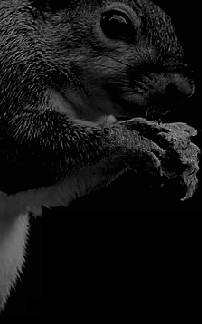
\includegraphics{../../../images/head.png}
  \end{textblock}
  \begin{textblock}{}(7,10)
    \noindent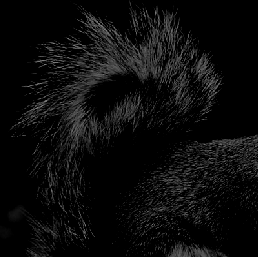
\includegraphics{../../../images/tail.png}
  \end{textblock}
  \maketitle
\end{titlingpage}

\pagecolor{white}
\mainmatter
\tolerance=400


\part{}

\chapter{The Center Kingdom}

\sections{The Missing Acorns}

A long time ago, when humans still lived in cities, on a cold morning
near the end of a long, cruel winter, in magnificent Central Park in
the middle of magnificent New York City, a young squirrel named Patch
was awakened very early by the growls of his empty stomach.

A squirrel’s home is called a \emph{drey.} Patch’s drey was very
comfortable. He lived high up an old oak tree, in a hollowed-out stump
of a big branch that had long ago been cut off by humans. The entrance
was only just big enough for Patch to squeeze in and out, but the drey
itself was spacious, for a squirrel. Patch had lined his drey with dry
leaves, grasses and bits of newspaper. It was warm and dry, and on
that cold morning he would have liked nothing better than to stay home
all day and sleep.

But he was so hungry. Hunger filled him like water fills a glass. The
cherry and maple trees had not yet started to bud; flowers had not yet
begun to grow; the juicy grubs and bugs of spring had not yet emerged;
and it had been two days since Patch had found a nut. Imagine how
hungry you would be if you went two whole days without eating, and you
may have some idea how Patch felt that morning.

\begin{tolerant}{1500}
Patch poked his head out of the drey, into the cold air, and shivered
as he looked around. Clumps of white, crumbly ice still clung to the
ground. Gusts of cold wind shook and rustled the trees’ bare
branches. The pale and distant sun seemed drained of heat. Patch took
a moment to satisfy himself that there were no dangers nearby, no hawk
circling above or unleashed dog below. Then he emerged from his drey
and began to look for acorns.
\end{tolerant}

But what marvels, what miracles, what mysteries are hidden within
those simple words!

\begin{tolerant}{500}
Squirrels are extraordinary creatures. Think first of how they
climb. When Patch left his drey, he went up, not down. He passed the
drey of his friend and neighbour Twitch, climbed to the northernmost
tip of his oak tree’s cloud of barren branches, and casually hopped
onto the adjacent maple tree, home to his brother Tuft. To a squirrel,
every tree is an apartment building, connected not only by the grassy
thoroughfares of the ground but by sky-roads of overlapping
branches. Tree trunks are like highways to them, even branches thin as
twine are like walking paths, and they leap through the sky from one
tree to another like circus acrobats.
\end{tolerant}

\begin{tolerant}{1000}
When he reached the last of the thick grove of trees, Patch paused a
moment to look around and consult his memory. His memory was not like
yours or mine. Human memories are like messages written on crumbling
sand, seen through warped glass. But squirrels have memories like
photograph albums; exact and perfect recollections of individual
moments. Patch, like every squirrel, had spent the past autumn burying
hundreds and hundreds of nuts and acorns, each one in a different
place. And he had stored all of those places in his memory book. The
winter had been long, but Patch’s memory book still contained a
precious few pages that depicted the locations of nuts not yet dug up
and eaten. He climbed to a high branch, stood on his hind legs, and
looked all around, seeking an image from one of those memories.
\end{tolerant}

If you had looked at Central Park that morning with human eyes, you
would have seen concrete paths, steel fences, a few early-morning
joggers and dog walkers, all surrounded by fields of grass and ice and
bare trees and rocks, and beyond them, Manhattan’s endless rows of
skyscrapers.

But with Patch’s eyes, with \emph{animal} eyes, he saw no park at
all. Instead he saw a city in itself. A vast and mighty city called
the Center Kingdom. A city of trees, bushes, meadows and lakes; a city
scarred by strips of barren concrete; a city surrounded by endless
towering mountains. All manner of creatures lived in this
city. Squirrels in their dreys, rats and mice in their underground
warrens, raccoons in the bushes, fish and turtles in the lakes, birds
fluttering through the trees or resting in their nests. At that hour
on that day, very early on a winter morning, the Center Kingdom was
almost abandoned — but soon spring would come, and the city would
bloom into a thriving maelstrom of life and activity. All Patch needed
to do, until that blessed time arrived, was find enough food for these
last few days of winter.

\begin{tolerant}{1000}
He saw in the distance, near the edge of the densely wooded area he
called home, a jagged rock outcropping from his memory book. He was so
hungry he paused only a moment to check for dangers before racing
headfirst down the tree trunk and towards the rocks. In his memory
that same outcropping was just \emph{there} — and the nearest human
mountain visible over the treetops to the west was \emph{there} —
and a particular maple tree, which had been covered in orange and
scarlet leaves on the day Patch buried the acorn, had been exactly
\emph{there,} and \emph{that} far away.
\end{tolerant}

Patch found his way to the exact spot where all those landmarks fell
into place, so that the place where he stood and the page from his
memory book matched perfectly, like a picture and its tracing. Then he
began to sniff. He knew as an undeniable fact that in the autumn he
had buried an acorn within a tail-length of where he stood. And
squirrels can smell perfume in a hurricane, or a dog a half-mile
upwind, or a long-buried acorn.

But Patch smelled nothing but grass, and earth, and normal air-smells.

His heart fell. It seemed to fall all the way into his paws and seep
out through the tips of his claws. Patch let out a little murmur of
awful disappointment. There was no food here. This acorn was gone,
already gone.

\begin{tolerant}{500}
This was not unusual. Squirrels often found and ate nuts buried by
other squirrels. But the same thing had happened with every nut Patch
had tried to unearth for the last two days. And that \emph{was}
unusual. It was such an astonishing run of bad luck that Patch had
never heard of such a thing happening before.
\end{tolerant}

He dug anyway, hoping that maybe this acorn had no smell, or his nose
was not working right. But he found nothing. And when he found the
next burial place, again there was nothing. He ran to the next; and
the next; until finally there were no more pictures left in Patch’s
book of memories, no nuts left to try to unearth. And he was so
hungry.

\begin{tolerant}{500}
By this time other squirrels too had emerged from their dreys and
begun to dig for food. Patch knew all of the half-dozen squirrels he
could see around him, and the dozen more whose presence he could smell
in the cold wind. All were of his tribe.
\end{tolerant}

Squirrels are social animals, they have family and friends, clans and
tribes and kingdoms. Patch’s tribe, the squirrels of the Treetops,
were not like the Meadow tribe who lived near the city’s grassy
plains, or the Ramble tribe that inhabited its rockiest wilderness, or
the red Northern tribe. The Treetops tribe was more a group of
individuals than a community. If they had had a motto, it would have
been, “Take care of yourself.” None of the squirrels around Patch were
of his clan. It would have been a terribly low and shameful thing for
Patch to go to one of them and ask for even a single bite of an
acorn. But while pride is important, it cannot be eaten, and hunger is
more important still. Patch was so ravenous he would have begged for
food.

But there was no one to beg from. For not a single one of the
squirrels around him had found a nut. All of them were digging for
nothing.

Patch sat and thought.

\begin{tolerant}{1500}
He was, you must remember, a squirrel, an animal, a creature of
instinct. Thinking did not come naturally to him. He had to sit for a
long time while he thought, in a little fenced-in patch of grass near
to one of the concrete-wasteland human trails. Around him there was
little to see. In winter most birds flew south, rats stayed
underground, raccoons hibernated. There were only the other hungry
squirrels, a few fluttering pigeons, and the occasional passing human.
\end{tolerant}

At one point an unleashed dog came near, and Patch had to interrupt
his thinking to watch this threat. It was a very strange dog. If it
was indeed a dog at all. It \emph{looked} like a dog, but it was
unaccompanied by any human, and it had a rich, feral scent like no
other dog Patch had ever encountered. The dog-thing said nothing,
which was also unusual, but it watched Patch with a leery grin full of
sharp teeth for what felt like a long time. Patch was very glad of the
fence that surrounded him. When the dog-thing finally moved on Patch
sighed with relief. He could have escaped to the safety of a nearby
tree if necessary. But he was so hungry that the effort of running
away, combined with the terrible strain of thinking, would have left
him weak and dizzy.

By the time Patch finally finished thinking, he had drawn one
conclusion and made two decisions.

\begin{tolerant}{1500}
The conclusion was that something was very strange and wrong. It was
not Patch alone who had lost all of his food. That would have been bad
enough. But the same thing seemed to have happened to every member of
his tribe. That could not be mere ill-luck. Something more, something
worse, was happening. There were dark stories told in whispers among
squirrels, ancient legends of winters that had outlasted all the
Center Kingdom’s buried nuts, famines in which nine in every ten
squirrels had died of hunger, and the few survivors had been forced to
eat the bodies of the dead in order to live. But there were no legends
in which all buried acorns had vanished uneaten from the earth. This
was something new.
\end{tolerant}

The first decision he made was that he would seek out his family, and
see if they had any food. Patch was solitary by nature, and had not
seen his family or indeed spoken to any other squirrel for three days,
but he knew they would help him if they could, just as he would help
them.

His second decision was that if his family did \emph{not} have food,
then … he would try something else. Something very unusual, for a
squirrel. Something very daring and dangerous indeed. But by this time
hunger was growing stronger in Patch than fear.


\sections{Patch’s Family}

Patch’s mother was named Silver, because high summer sun made her fur
shine that colour. She had a marvellous drey high up a spruce tree,
carved out long ago by a woodpecker, and since extended into a
two-chambered home full of bright things. The journey along the
sky-road to her drey did not take long. When Patch looked inside, he
saw a hundred colours glittering in the sunlight, shining from bits of
metal and glass set into Silver’s walls and floor. But his mother was
not there.

He could tell by the faintness of her smell that no squirrel had been
here in some time. There were two faint traces of scent, several days
old; that of Silver, and that of another squirrel, a musky scent that
Patch did not recognize. A scent that made his tail stiffen as if
danger was near.

Patch stared into his mother’s empty drey for a moment. It wasn’t
normal for a squirrel to abandon her drey for days, not in the middle
of winter. And he hadn’t seen Silver for three days. Not since all the
acorns had disappeared from the earth.

Patch ran back to his own tree, and then to the maple tree next door,
to his brother Tuft’s drey. He ran very fast. He was hungrier than
ever, and he was beginning to be very worried. He was relieved when he
looked into Tuft’s drey and found it occupied. Tuft himself was not
present, but Brighteyes was, and their babies, and it was clear from
the smells that Tuft had only just departed.

“Hello, Patch,” Brighteyes said weakly. “Would you like to come in?”

\begin{tolerant}{1500}
Patch entered. Brighteyes was curled up with her babies in the drey’s
deepest, warmest corner. The last time Patch had visited, seven days
ago, this had been a den of noise and chaos, with all Brighteyes’ four
babies running and jumping and playfighting. Today they lay weakly
beside Brighteyes, and the once-shining eyes from which their mother
had taken her name were dim and clouded.
\end{tolerant}

“Uncle Patch,” the littlest baby said, in a piteous mewling
voice. “Please, Uncle Patch, do you have any food?”

The other children looked up at Patch with bright, hopeful eyes. As
hungry as he was at that moment, if he had had an acorn, he would have
given it to his nieces and nephews. But he had nothing.

“I’m sorry,” Patch said, ashamed. “I haven’t found any food for days.”

“No one has,” Brighteyes said.

“Have you seen Silver?”

“No. She hasn’t come to visit since the food ran out.”

Patch considered. “Is Tuft out looking for food?”

\begin{tolerant}{1500}
After a long moment Brighteyes said, very quietly, as if she were
admitting something terribly shameful, “Tuft has gone to the Meadow
tribe.”
\end{tolerant}

\begin{tolerant}{5000}
“The Meadow tribe?” Patch asked, confused. “What for?”
\end{tolerant}

Brighteyes said in a voice hardly louder than a whisper, “To accept
their offer.”

“What offer?”

Brighteyes stiffened with surprise. “You haven’t heard?”

“Heard what?”

“You spend too much time on your own, Patch. If you talked to others
more you wouldn’t always be the last to know.”

“The last to know \emph{what?}”

“The Meadow tribe has offered food to Treetops squirrels. But only if
we join their tribe.”

“Join their tribe?” Patch looked at her, perplexed. “Join the Meadow?
That’s not possible. We’re of the Treetops. We can’t become of the
Meadow.”

“They say if we swear an oath of allegiance to the Meadow tribe, if we
swear by the moon, then we will become of the Meadow, and then they
will give us food.”

After a long moment, Patch asked, his voice now as hushed as that of
Brighteyes, “Swear by the moon?”

This is not the place to explain what the moon means to
animals. Suffice to say that an oath sworn by the moon is even
stronger than an oath sworn on blood. Such an oath can never be broken
or unsworn.

“Yes,” Brighteyes said, looking away from Patch.

“Tuft has gone to swear by the moon to join the Meadow tribe?”

“Yes. We will all go. We will all swear. Tuft will bring back some
food for the children, and when they are strong enough they will go
and swear themselves.”

\begin{tolerant}{500}
“You can’t do this,” Patch said, shocked. “You can’t leave the
Treetops. You can’t give your children to another tribe.”
\end{tolerant}

“We must. We haven’t any \emph{food,} Patch. You see how weak my
babies are. No one else can help us. Silver is gone. Jumper is gone.”

“Jumper is gone? Gone where?”

“No one knows. No one has seen him in days. Like no one has seen
Silver. Or any of the other clan leaders.”

“The King,” Patch said. “We’ll go to King Thorn.”

“The Ramble is too far. Even if the King sends help, it will never
reach us in time. My babies are starving, Patch. My babies are
\emph{dying.} The Meadow is our only hope.”

After a moment Patch turned away, unable to face Brighteyes, and said,
“I wouldn’t have let this happen to you.”

“Don’t say that. There’s nothing Tuft could have done. There’s nothing
you could have done if I had chosen you instead.”

“There is. If I had known. I know another place to get food.”

“Then why are you hungry?” Brighteyes asked.

Patch hesitated. “It’s dangerous. It’s in the mountains.”

“In the \emph{mountains?} Are you \emph{mad?}”

Patch was saved from answering by the appearance of his brother Tuft
at the entrance to the drey. Tuft held two acorns against his chest,
but he looked perilously thin, and weak, and tired.

“It’s done,” Tuft said. His voice was grim. “I have joined the
Meadow.”

Tuft carried the food in to his family. As the children devoured one
acorn, Brighteyes and Tuft and Patch stood around the other, staring
as if it glowed.

“This one is for you,” Tuft said to Brighteyes. “The Meadow gave me
one for myself when I was there.”

Patch knew Tuft was lying.

Brighteyes said, “We’ll share it. All three of us.”

Patch wanted a bite of acorn so much that his whole body trembled with
desire.

“No,” he said faintly.

Tuft and Brighteyes turned to him, amazed.

“I will go to the mountains,” Patch said.

Right away, before the acorn’s temptation became too great to deny, he
turned and fled from his brother’s drey, and ran straight down the
maple trunk to the ground. From there Patch ran north and west. His
hunger was a searing flame within him.


\sections{Patch and the Birds}

It was not entirely true that Patch \emph{knew} there was food in
the mountains. He had never been to the mountains. No squirrel in all
the Center Kingdom, as far as he knew, had ever been to the
mountains. For between the kingdom and the mountains, surrounding it
on all sides like a moat around a castle, there lay a blasted concrete
wasteland, as wide as fifty squirrels laid nose to tail, and horrific
death machines roared up and down this wasteland at terrifying speeds,
all day and night. What’s more, humans and dogs often crossed between
the mountains and the kingdoms; and sometimes the dogs were
unleashed. A squirrel would have to be very desperate indeed to dare
the wastelands.

It was Toro who had told Patch about the food in the mountains. Toro
was Patch’s friend. And that itself was extraordinary.

Patch had always talked to birds. The drey he had grown up in —
Silver’s old drey, before she became leader of the Seeker clan — had
been only a few branches away from a nest of robins. Once, in early
spring when he was still a baby, Patch had crawled out of Silver’s
drey and into the robin’s nest, and had spent a whole day among the
chicks before Silver returned home and retrieved him. The robin mother
had been unamused by Silver’s profound apologies, and even less amused
when Patch returned to her nest the very next day.

Eventually Silver taught Patch to leave the robins alone, but not
before he had learned how to speak Bird. Most squirrels of the Center
Kingdom could say and understand a few simple things in Bird, but
Patch could actually hold conversations. And so, one autumn day when a
bluejay swooped past and stole an acorn out of Patch’s paws, Patch
shouted angrily at the thief in Bird to bring it back; and the thief,
intrigued, wheeled around in midair, perched on a branch above Patch,
and looked curiously down at the irate squirrel.

\begin{tolerant}{5000}
“Thieving feather-brained no-nose hawkbait!” Patch shouted up.
\end{tolerant}

“Stupid blind furry groundworm!” the bluejay retorted, and began to
peck at the acorn.

“Your mother should have dropped your egg onto a rock!”

“I must say,” the bluejay said between bites, “you speak Bird
remarkably well, for a thick hairy slug with a mangy tail.”

“Thank you, you moldy-feathered sky-rat. Now give me back my acorn!”

The bluejay considered, while he finished eating half of the
acorn. And then, rather incredibly, he let the other half drop to the
ground.

“To tell you the truth I wasn’t very hungry,” he said. “I just enjoy
taking acorns from squirrels. I didn’t know you spoke Bird. What is
your name?”

“My name is Patch.”

“My name is Toro.”

Patch didn’t know what to say. He had never been introduced to a
bluejay before. Like all squirrels he thought of bluejays, the Center
Kingdom’s most prolific eaters of nuts, as dire enemies. Patch looked
around to see if any other squirrels saw him talking to a
bluejay. Fortunately none were nearby.

\begin{tolerant}{1000}
“If you’re looking for acorns,” Toro said, “the wind has been strong
today on the other side of those rocks, and many there have fallen.”
\end{tolerant}

After a moment Patch said, stiffly, “Thank you.”

“Any time,” the bird said carelessly, before flying away.

\begin{tolerant}{1000}
That was the beginning of their secret friendship. It had to remain
secret, for other squirrels would have been enraged by the thought of
Patch befriending Toro, and other bluejays would have looked askance
at Toro befriending Patch. But the two had much in common. Both were
lone explorers. And when they saw one another in remote corners of the
Center Kingdom, as they often did, they stopped to talk. It was during
one of those conversations, in the depths of the winter, that Toro
told Patch of what his sharp bluejay eyes had seen in the nearby
mountains.
\end{tolerant}


\sections{In The Mountains}

\begin{tolerant}{1000}
Patch stood beneath the tree that marked the absolute edge of the
Center Kingdom and stared horrified at the wasteland between himself
and the mountains. Death machines hurtled past in both directions,
roaring and snarling, zooming by at speeds so great that Patch could
feel the wind of their slipstreams. Sometimes they stopped for a few
moments to gather in packs; then they all leapt into motion at
once. On either side of the wasteland, metal tree trunks protruded
from the concrete, and from their glistening branches hung
ever-changing lights. Patch knew from previous experimentation that he
could not climb these metal trees. Even a squirrel’s claws found no
purchase on their smooth and shining bark.
\end{tolerant}

At least he saw no dogs, and only a few humans. But from where he
stood his intent seemed not just dangerous but actually insane. Surely
it was better to abandon the Treetops and swear allegiance to the
Meadow than to leap into the certain death of the wasteland. Patch
turned around and took a few steps back towards Tuft’s drey.

Then he stopped, turned back, cocked his head, and looked once more at
the wasteland. He had just realized there was something rhythmic about
the way the death machines moved. There was a \emph{pattern.} The
same pattern as that of the changing lights in the sky.

\begin{tolerant}{1000}
He thought of what Toro had told him. Heaps and rivers of food,
waiting to be eaten. Patch couldn’t smell any food. He could hardly
smell anything over the foul belches of the death machines. The death
machines that stopped when the lights changed, maybe, just maybe, long
enough for a squirrel to scamper across the wasteland.
\end{tolerant}

\begin{tolerant}{500}
Hunger plays tricks on the mind. By the time Patch realized he was
actually running for the mountain, and not merely considering it, he
was already halfway across the wasteland. The concrete beneath his
paws was hard and cold. The several humans on the mountain side of the
wasteland had ceased their motion and turned their heads to look at
Patch. That wasn’t good. But he had gone too far to turn back. The
death machines would crush him if he did. His only hope was to keep
running. He ran so hard and so fast that after crossing the wasteland
he very nearly ran headfirst into the nearest mountain.
\end{tolerant}

Patch stopped just in time and looked around, breathless, amazed at
what he had just done. Having reached his destination he did not know
what to do next. This was a new and alien world. The ground was
entirely concrete; he couldn’t see a single blade of grass on this
side of the wasteland. The mountain before him was a perfectly
vertical wall of rock that reared into the sky far higher than any
tree. There was wasteland on two sides; behind him, the wide barrier
he had just crossed, teeming with death machines, and to his right, a
narrower offshoot that ran deeper into the mountains, occupied only by
stationary death machines along its edges. Patch wondered if they were
dead or only sleeping. He hoped for dead. At least there were a few
trees along the side of this narrow wasteland, although they were
small and withered, their trunks were caged with bricks, and they were
spaced so far apart there was no sky-road. Between some of the trees,
in the distance, Patch saw a few piles of what looked like big, shiny
black rocks.

There were no other animals, only a few passing humans. But while
these humans did not approach Patch, they seemed to be directing their
attention towards him. This made him very nervous. Humans were huge
and unpredictable. Some humans who entered the Center Kingdom spilled
food all around them, but the younger ones often tried to attack
squirrels, and all of them smelled extraordinarily strange.

\begin{tolerant}{1000}
Patch sniffed the air. Beneath the thick acrid fumes of the death
machines and the alien scent of humanity, he smelled danger. He
smelled dogs. Upwind, to the north, across the narrow wasteland, three
large dogs leashed to an old human were approaching. Patch hoped the
wasteland would forestall them — but as he watched, the dogs began to
cross. And then the lead dog saw Patch, and its eyes lit up like
flames.
\end{tolerant}

“Kill you and eat you!” it howled ecstatically. “Kill you and eat
you!”

The other dogs joined in. “Kill you and eat you! Kill you and eat you!
Kill you and eat you!”

Patch didn’t stop to listen. Dog conversation was always the
same. Patch scrambled for the nearest scrawny tree, and raced right up
to its crown.

“Kill you and eat you, kill you and eat you, kill you and eat you!”
the dogs shrieked at him, while they tried to pull their human towards
the tree. But the human, while old, was still a massive creature, and
to Patch’s relief it pulled the homicidal dogs along until they
vanished behind the corner of the mountain.

Patch looked around. He stood atop a sickly tree, surrounded by
mountains and wasteland. Beneath him, a death machine shuddered into
motion and roared forward, and Patch realized to his horror that all
those motionless machines were not dead, only sleeping, and might come
to life at any moment.

\begin{tolerant}{500}
Patch was starving, but worse, he was so terrified he could hardly
move. He wished with all his heart he had never crossed the wasteland
into the mountains. He saw and smelled no food here. And he did not
dare descend from this scrawny tree. There was no safety
below. Between the mountains and the line of death machines beneath
him there was a slightly raised strip of concrete, in which the trees
were set; but it was perfectly apparent to Patch that the death
machines, with their terrible rolling feet, could easily rampage down
this narrow strip too if they so desired. Nowhere and nothing in the
mountains was safe.
\end{tolerant}


\sections{A Welcome Discovery}

“Patch!” a voice chirped. “Patch, is that you?”

Patch looked to the sky and his heart filled with relief as a bluejay
fluttered downwards and settled on a nearby branch. Nothing dispels
fear like the unexpected arrival of a friend.

“What are you doing here?” Toro asked, amazed.

“I came to get food,” Patch said. “You said there was food here.”

“There is. Just down there.” Toro pointed with his beak deeper into
the mountains. “Inside those black things. Around them too,
sometimes.”

“The rocks?” Patch asked doubtfully, but as he looked, he saw the
skins of what he had taken to be rocks fluttering in the cold wind.

“Some of them are full of food. Food falls right out of them. Go on
down, I’ll show you.”

“Go on down,” Patch said, even more doubtfully.

“It’s perfectly safe. Just follow me,” Toro said.

The bluejay launched himself into the wind, angled his wings into a
slow gliding turn, and came to rest on the concrete, next to where a
heap of black things stood beside one of the caged little trees.

“Easy for you,” Patch muttered. “You’re a bird. You just fly away from
trouble.”

\begin{tolerant}{700}
But the sight of his friend perched casually right next to a sleeping
death machine, combined with the promise of food, was enough to bring
Patch down to the concrete. He scampered towards Toro as quickly as
possible, turning his head from side to side to look for danger. He
found it everywhere. There were humans both behind and ahead of Patch,
a row of sleeping death machines to his right, and to his left he
smelled rats. Many rats.
\end{tolerant}

“This is it!” Toro said when Patch reached him.

\begin{tolerant}{500}
Toro sounded as proud as if he stood before a hill of acorns as high
as a human, rather than a pile of huge, foul-smelling black things
like seed-pods, their shiny skins flapping like leaves in the
wind. Patch looked skeptically at the trickled heap of decaying sludge
beneath one of the seed-pods, and said, “You said there was
\emph{food.}”
\end{tolerant}

“There’s food inside them,” Toro promised. “Just go inside. That’s
what the rats do.”

“It’s rat food?” Patch asked, horrified. Rats would eat anything, the
more rancid and disgusting the better.

“Rats come here,” Toro admitted. “That’s how I found it, I saw
them. But sometimes it’s good food too. Once, right here, I found the
most marvellous seeds I ever tasted. They were wonderful.”

Patch sniffed the air. He smelled bluejay, death machines, rotting
sludge and rats. He smelled his own fear and hunger. But there was
something else beneath all that. Like the faintest hint of wine in
muddy water, or a musical phrase almost drowned out by a howling
crowd, Patch smelled something so delicious that his mouth began to
water.

“What is it?” Toro asked.

“It’s here,” Patch said. He leaped up on the nearest black thing. Its
material had a strange slick feel, made an alarming crinkling noise
when he landed, and was so soft his claws tore right through it. Patch
jumped to the top of the pile of huge black seed-pods, and ripped open
the skin of the uppermost one with a few bites. The wonderful smell
was suddenly stronger. Patch hesitated only a moment. Then he dove
headfirst into the hole he had made.

It was so dark inside the seed-pod that he could not see. His snout
encountered dry fluttery things, wet sticky things, even hard metal
things. In his hunger he pushed them all aside, squirming deeper and
deeper, following his nose towards the smell that made him dizzy with
hunger. He found paper, like the newspaper with which his drey was
lined. He tore the paper open with his teeth. And inside he found a
whole mound of food like nothing Patch had ever tasted before. It was
soft, salty, and delicious. There was enough to fill the bellies of a
dozen squirrels.

Patch ate, and ate, and ate.

\begin{tolerant}{500}
Until dimly, through all the debris that surround\-ed him, he heard
Toro’s high, harsh cry that meant: “Danger!”
\end{tolerant}


\sections{A Promise}

When Patch finally found his way out of the seed-pod, Toro was gone,
and there were rats all around him. Some hid beneath the huge black
seed-pods, some scuttled in the shadows of the nearby mountain. Patch
knew from their smells there were at least a dozen of them.

There was another smell too, mixed with that of the rats. The very
same unsavory squirrel-smell he had detected in Silver’s abandoned
drey.

\begin{tolerant}{1500}
“What do you want?” Patch asked, from his perch atop the mound of
seed-pods. He was concerned but not yet frightened. Rats and squirrels
were neither friends nor enemies. Squirrels were bigger and stronger,
but rats were far more numerous. There were legends of long-ago wars
between the two species, but no squirrel Patch knew had ever been
attacked by rats. Squirrels lived aboveground, in the sun; rats
frequented the night and the dark underworld. Of course, squirrels
found rats disgusting and disagreeable — but so did all other animals.
\end{tolerant}

An unusually large rat climbed up to the top of a seed-pod. It was
almost as big as Patch himself. Rats usually avoided light, but this
one stood unafraid beneath the sun, and demanded: “Who are you?”

“I am Patch son of Silver, of the Seeker clan, of the Treetops tribe,
of the Center Kingdom,” Patch said. “Who are you that asks?”

“I am Snout,” the rat replied. “Why are you here?”

“I came to look for food.”

“This is our food. These mountains are ours.”

“Your food?” Patch asked, bewildered. There was no ownership of food
in the Center Kingdom, not until it had actually been eaten. “That’s
ridiculous. It’s food. It belongs to whoever finds it first.”

“Then you belong to us,” Snout hissed. “Because we are the rats who
will suck the marrow from your broken bones.”

And from the shadows all around the heaped seed-pods, other rats
arose, and began to climb towards Patch at the top of the pile.

Patch didn’t hesitate. He sprinted downwards, running straight at one
of the rats. His charge was so unexpected that the rat in question
stopped and shrank away a little, just enough for Patch to scamper
past him, towards the edge of the pile. Two more rats raced out from
beneath the mountain, blocking any escape across the concrete. He was
still surrounded, rats were scuttling towards him from all directions.

\begin{tolerant}{1000}
From the very edge of the pile of seed-pods, Patch jumped as high and
as far as he could. For a moment, in midair, he was sure he wouldn’t
make it, he would fall to the concrete and be torn apart by the rats —
but then his outstretched claws latched onto the bark of the little
tree beside which the seed-pods had been heaped. Moments later he was
on top of the tree, looking down at the milling figures of more than a
dozen frustrated rats.
\end{tolerant}

“Come on up!” Patch cried out cheerfully.

\begin{tolerant}{2000}
He wasn’t as confident as he sounded. Rats weren’t near as nimble as
squirrels, but there were many of them, and this was a very small
tree. If all the rats climbed up, Patch wasn’t sure he would
escape. But at least he was up a tree, his belly was full for the
first time in days, and Toro was watching from the next tree over.
\end{tolerant}

\begin{tolerant}{1000}
“I will find you, Patch son of Silver,” the rat named Snout
promised. “I will find you and eat your eyes from your skull.”
\end{tolerant}

\begin{tolerant}{2000}
Patch said nothing. He only watched as the rats scurried away. Most of
them returned to the shadows at the base mountain. But Snout ran along
the edge of the mountain, until he reached a huge hole in the
mountain’s side. Humans had blocked the hole with a wire fence much
like those in the Center Kingdom. Snout squeezed himself through a
hole in the fence and disappeared into shadow.
\end{tolerant}

“Did you find food?” Toro asked.

“Yes,” Patch said. “It was wonderful.”

“I’ve never seen rats like that before.”

“Neither have I.”

“You should go back to the Kingdom. It’s safe there.”

Patch was afraid to stay in these terrible mountains for even a moment
longer. He wanted to run back to the Center Kingdom, with his full
belly and his wonderful story of adventure that no other squirrel
would ever believe, and wait for spring to come. But he thought of his
mother’s empty drey, and the haunting squirrel-smell there — and the
way that very same musty squirrel-smell had emanated from that biggest
rat.

“Not yet,” Patch said.


\sections{Jumper}

\begin{tolerant}{2000}
The opening in the wire fence that Snout had squeez\-ed through was too
small for Patch to do the same. But it was easy enough to climb up to
the top of the fence. From there, Patch could see all of the hole in
the side of the mountain. It was like some enormous creature had taken
a big bite from the mountainside. Beneath the wire fence, a
sheer-walled pit plunged deep into darkness. The pit was full of human
things, metal and concrete shaped in the strange curves and straight
lines that humans favoured but made animals feel queasy. The air was
dusty and smelled awful. Patch shaded his eyes with his tail and
squinted, but from the top of the fence, where the sun shone brightly,
he could still not see into the darkness at the pit’s bottom.
\end{tolerant}

“I think we should go,” Toro said.

“Not yet,” Patch repeated. He watched the dust clouds in the pit, the
way they moved. He didn’t want to be upwind of the rats. They too had
sharp noses. He ran along the top of the fence, as far downwind as he
could, and then he took a deep breath and ran straight down the fence.

The lip of the pit was hard concrete, no good for downclimbing, but a
wooden plank ran down into the shadows. Patch moved down this plank as
quietly as he could; rats had sharp hearing, too. It was strange to
walk on wood with such a perfectly straight surface. The pit was as
deep as a medium-sized tree. About halfway down the plank he moved
from sunlight into shadow, and his eyes began to adjust to his new
surroundings.

The center of the pit was jumbled full of huge, geometric human
things. Its bottom was crisscrossed by pipes and planks and
girders. The floor and one wall of the pit were rocky earth rather
than concrete. But it was in a corner between two concrete walls,
towards the inside of the mountain, that he saw the unmistakable
scuttling motion of a rat.

Patch crept closer, staying behind human things as much as
possible. He reached a metal pipe that ran near the corner, and
followed its length until the pipe ran into the concrete wall, just a
half-dozen squirrel-lengths from the corner. He was still downwind, he
thought, although it was difficult to read the wind down here. Patch
stood as high as he could and was just barely able to look over the
pipe and see into the corner of the pit.

In that corner Patch saw something very strange. He saw a dozen large
rats standing in a circle, all facing outwards, with all their tails
knotted together in a big tangled lump in the middle of their
circle. Standing on this lumpy knot of tails was Snout, the biggest
rat of all. And next to this bizarre clump of rats, Patch saw, to his
great surprise, another squirrel, small and with reddish fur.

“Patch son of Silver,” the strange squirrel said, and Patch
stiffened. “I’ve heard of him. He’s of the Treetops. He talks to birds
and goes off alone for days. I’m sure he doesn’t know anything. He
just came to the mountains for the food.”

“That’s not good enough,” Snout said. “We will give him to Karmerruk.”

“But —” the squirrel began.

“We will give him to Karmerruk.”

The name meant nothing to Patch, but it seemed to frighten the
squirrel.

“You said you would show me Jumper,” the squirrel said hesitantly to
Snout.

Patch stiffened.

\begin{tolerant}{500}
“Oh, yes, Jumper,” Snout said, and smiled, revealing jagged yellow
teeth. Then, loudly, the rat commanded, “Bring him!”
\end{tolerant}

There was a dark hole in the corner of the pit, near where the rats
and the other squirrel stood. Patch saw motion in that hole. He saw a
squirrel’s head emerge. He watched, shocked, as Jumper, lord of the
Treetops tribe, crawled painfully out of that hole, his motions slow
and spastic, and fell clumsily to the ground. Jumper was bleeding in
many places, and he pulled himself along with his forelegs alone; both
his hind legs hung motionless from his body. Several rats followed
Jumper out of the hole.

“Lord Jumper won’t be jumping any more,” Snout said, and laughed.

Jumper pulled himself up on his forelegs. Patch could see he was in
great pain.

“Redeye,” Jumper said in a ragged voice, to the squirrel who stood
among the rats. “How can you have you done this?”

The other squirrel looked uneasy, and didn’t answer. Patch was glad to
have his name. It was Redeye he had smelled in Silver’s drey.

“He did it for me,” Snout said. “He has sworn to serve me, as I have
sworn to serve the King Beneath. The king in whose name you and all
your kind will die and be devoured.”

Snout stepped away from the knot of rat-tails on which he stood. The
knot began to squirm like a nest of worms as the rats untied
themselves from one another. As they were released the rats formed
into a tight circle around Jumper. Snout joined the circle. So did
Redeye. Patch knew what would happen next. He didn’t want to
watch. But it was too awful a thing to turn away from.

“No,” Jumper begged them. “No, please. Not like this.”

“Yes,” Snout hissed. “\emph{Exactly} like this.”

\begin{tolerant}{500}
And then they swarmed the crippled lord of the Treetops. Jumper howled
three times before he fell silent beneath the frenzied mass of biting
rats. Redeye seemed more rat than squirrel as he tore at Jump\-er’s body
with his sharp fangs. In scarcely more time than it takes to tell it
there was nothing left of Jump\-er but scraps, bones, and a puddle of
blood. Even then the rats began to gnaw on Jumper’s bones and lick his
blood. They would leave nothing of him at all.
\end{tolerant}

\begin{tolerant}{500}
Patch retreated silently to the wooden plank that led out of the
pit. He felt colder than he had on the worst day of the winter. The
squirrel Redeye had betrayed Jumper to rats, helped to kill him,
helped to \emph{eat} him. And Redeye’s scent had been in Silver’s
drey. Patch climbed numbly into the sunlight, over the fence, back to
the concrete, heedless of the passing humans and the death
machines. They held scarcely any terror for him now; all he could
think about was what he had seen in the pit below.
\end{tolerant}

“What did you see?” Toro called out, from a tree. “What was down
there?”

Patch said, “I have to go back to the Kingdom.”


\sections{To The Meadow}

\begin{tolerant}{1000}
Returning to the Center Kingdom was relatively easy, now that Patch
knew how to cross the wastelands. He was relieved when he once again
felt grass beneath his paws. But he was also very worried, and he
immediately dashed for the maple tree next to his own. He was too
late. Tuft’s drey was empty; he and Brighteyes had already taken their
children to swear to the Meadow tribe.
\end{tolerant}

Patch considered a moment, and then he took the sky-road to his own
tree, and descended to the drey of his friend and neighbour Twitch. He
half-expected to find that Twitch too had gone to the Meadow. But
Twitch was in his drey, and Patch was very pleased to find that he was
not alone, but was with Patch’s oldest friend Sniffer.

“Patch!” Twitch cried out, excitedly jumping to his feet when he saw
Patch at the drey entrance. “Sniffer is here! Sniffer found me food!”

And indeed a chestnut and two acorns sat on the floor of Twitch’s
drey. It made sense that Sniffer, of all the Treetops squirrels, had
been able to find food. Sniffer had the sharpest nose in all of
Treetops, probably in all the Center Kingdom. It was said he could
smell a buried acorn from halfway up a tree.

“I brought it for you too, Patch,” Sniffer said.

“Thank you,” Patch said, “but I’ve eaten.”

Sniffer gave him a sharp look.

“You found food too?” Twitch asked. “Where? How was it? Was it acorns?
Was it chestnuts? Did humans bring it? Are the maples budding?  Oh, I
would love a nice fresh maple bud right now. I love nuts, you know I
love nuts, but it’s been only nuts all winter, I’d love a maple
bud. Or a fresh grub, oh, a nice juicy grub. Or best of all, a tulip
bulb, imagine, Patch, tulips! I just can’t wait for spring. What kind
of food did you find, Patch? Was it good? Is there more?”

\begin{tolerant}{2000}
Patch had to interrupt. It was difficult to get Twitch to stop talking
about food once he had started. Patch said, harshly, “Jumper is dead.”
\end{tolerant}

Sniffer and Twitch stared at him.

“He was eaten by rats,” Patch said. “And a squirrel named Redeye. In
the mountains. I saw it all. And Redeye was in Silver’s drey, I
smelled him there. Sniffer, do you think you can follow his scent?”

\begin{tolerant}{1000}
“Dead?” Twitch asked, still trying to understand. Twitch was bigger
and stronger and could run faster than any other squirrel in Treetops,
but he had never been able to understand things particularly
quickly. “Lord Jumper? Eaten by rats? In the mountains? You were in
the mountains?”
\end{tolerant}

“Yes,” Patch said.

“This is serious,” Sniffer said. “This is very serious.”

Patch inclined his head in agreement.

“Did you say Redeye?” Twitch asked. “I know Redeye. He’s of the
Meadow. He’s Gobbler clan. One of his eyes is red and he’s called
Redeye. Just like you have that white patch on your head and you’re
called Patch. And I twitch a lot and I’m called Twitch. And Sniffer —”

“Yes, thank you,” Sniffer interrupted.

When Twitch wasn’t talking about food, he often spent a lot of time
restating the very obvious. But Twitch did have a very good memory for
animals and their names. If Twitch said Redeye was a squirrel of the
Meadow, then it was certainly so.

“I’ll take you to Silver’s drey so you can know his scent,” Patch
said. “And then we’ll go to the Meadow. Maybe we can find him there.”

“It’s a long way to the Meadow,” Sniffer objected. “It’s cold. It
might be night before we can get back.”

“We can find a tree to stay in.”

Sniffer looked dubious.

“Please, Sniffer,” Patch said. “Silver is missing. Jumper is
dead. This is serious. You said so yourself.”

\begin{tolerant}{1000}
“Serious means dangerous,” Sniffer muttered. “All right. Just … just
let me go to my drey and get a little more food. Twitch can eat all
this himself. Then I’ll come back here and we can go to Silver’s drey
and to the Meadow.”
\end{tolerant}

“Thank you,” Patch said, but Sniffer did not stay to hear his
thanks. Sniffer’s tail was already disappearing out the entrance to
Twitch’s drey. Sniffer did not usually move so quickly. Patch supposed
he wanted to hurry to make sure they could get back before night.

“Tell me about the food in the mountains,” Twitch said eagerly.

“Not now, Twitch,” Patch said distractedly. “You should eat. It’s a
long way to the Meadow. You need your strength.”

Patch was thinking about what might have happened to Silver, and at
the same time, he was trying \emph{not} to think about what might
have happened.

Twitch looked at his chestnut and two acorns. Then he looked at Patch,
and said, in a tense, strained voice, “Would you like some?”

“No, thank you,” Patch said.

Twitch grinned with relief and fell to his dinner. By the time Sniffer
got back there was nothing left of the three nuts but their shells.

\begin{tolerant}{1000}
They had a long way to go. In general, the Treetops tribe was spread
across the western section of the Center Kingdom, the Meadow tribe was
in the south, the Ramble tribe was in the center and the east, and the
Northern tribe inhabited the kingdom’s farthest northern
reaches. There were exceptions, such as a colony of Meadow squirrels
just north of the Great Sea, and those Treetops settlers who lived in
the north; but Patch and his friends lived in the heart of Treetops
territory. A journey to the green fields of the Meadow and back would
occupy at least half a day. Much of the journey required ground travel
rather than the sky-road, and that meant warily crossing concrete
strips, avoiding dogs and humans, checking the skies for danger, and
so forth.
\end{tolerant}

But it was not while they were on the ground that danger struck. It
struck instead when Patch, Sniffer and Twitch were in a dense cluster
of cherry trees, travelling rapidly along the sky-road to the
south. They did not hear a flutter of wings. They did not see a dark
shadow streak along the ground towards them. The first they knew of
the red-tailed hawk was when it seized Patch with talons sharp as
broken glass and snatched him up from the cherry tree, carried him
screaming into the sky to be killed and eaten.


\sections{Animal Language}

A brief word is perhaps in order on the subject of animal languages.

I have already made it clear, I hope, that animals do not think in the
way that you and I do. It should not surprise you to learn that they
do not speak like humans either. In fact sound plays little part in
the language of most animals. Many animals speak mostly with their
bodies, by moving their heads and limbs, and with pheromones,
chemicals released by special glands that long ago withered away in
humans.

There is of course no one animal language. There are as many animal
languages as there are animal species. It is true, however, that the
more similar the animal, the more similar their language. Squirrels,
chipmunks, rats and mice are all rodents, and can understand one
another very well. Dogs are not rodents, but they are mammals; a dog
and a squirrel could have a conversation, if it ever occurred to the
dog to say anything other than “Kill you and eat you!” It is fair to
say that, with a little effort, all mammals can speak Mammal to one
another — except for humans, who have lost all their powers of animal
speech, and the great apes, who understand sounds and motions but not
pheromones, and so are half-deaf and half-dumb.

Birds are another matter entirely. Birds are the descendants of
dinosaurs, more like reptiles than like mammals. Again, while all bird
species speak their own language, it is fair to say all birds can
speak Bird. But birds, like the great apes, do not use pheromones;
theirs is a language entirely of sounds and motions. It is because of
this that birds and mammals can only usually communicate a few basic
notions. Patch’s ability to speak Bird was quite rare. But since Bird
is half body language, you can imagine how difficult it was for him to
speak while his body was held by the hawk’s strong and terribly sharp
talons.

As for reptiles, there will be more to say of them in time.


\sections{A Bargain of Mice and Words}

Patch squirmed and wriggled, fighting for freedom, trying to break
free of the hawk’s vicious talons. He had already been carried higher
than the highest tree of the Center Kingdom; indeed he was higher than
many of the mountains, and he knew a fall might well kill him; but he
was small, and would not fall hard, and so escape from the hawk’s
claws meant at least a \emph{chance} of survival, compared to the
certainty of being eaten if he did not escape. So he struggled with
all his might. But the hawk was too strong. All Patch managed to do
was work the painful talons even deeper into his flesh.

Patch gave up and sagged limply. He was going to die. That was simply
all there was to it. Every animal had a time to die, and this was
his. He looked down at the Center Kingdom from high above. He had
never seen it like this before, a lush rectangle set amid the gray
mountains. The trees of the Center Kingdom looked as small as blades
of grass. He committed the striking image to his memory book before
remembering there was no point; soon he would be dead, and the dead
have no memories at all.

It occurred to Patch that it was very strange for a hawk to capture a
squirrel from a tree. Even in winter, hawks usually avoided diving
into trees, for fear of branches that might tear at their faces and
feathers. Hawks usually preyed only on animals in open spaces. Patch
had been extremely unlucky.

This realization made Patch so angry at the unfairness of the world
that he shouted out to the hawk, in broken sound-only Bird, “Why take
me from tree? Why not take squirrel on ground?”

The hawk was so surprised it nearly dropped him.

“You speak Bird?” the hawk asked, its voice rasping and imperious.

“Yes,” Patch said.

“You speak Bird,” the hawk repeated. It considered for a moment. “Well
then, my furry little lunch, let us speak a moment before I dine.”

The hawk changed course, headed for a conical turret atop one of the
mountains, and swooped into a perfect landing on a small, circular,
walled stone platform at the very top of the turret, a platform shaped
a little like a bird’s nest. It was only a few squirrel-lengths
across, and its smooth vertical walls could not be climbed. There was
no way for Patch to escape.

“What is your name, little squirrel?” the hawk asked, releasing Patch.

Patch stood to his full height, painfully, for he was bleeding from
the talon wounds, and said for what he expected was the very last time
in his life, “I am Patch son of Silver, of the Seeker clan, of the
Treetops tribe, of the Center Kingdom. Who are you that asks?”

“I am Karmerruk,” the hawk said proudly. “Now tell me, what have you
done to Snout, that he wants you dead so badly?”

Patch stiffened with surprise. “The rat,” he said, amazed. “You serve
the rat.”

Then he cried out as Karmerruk’s talons slashed his face.

“I serve no one and nothing,” Karmerruk said, his voice low and very
dangerous. “I am a Prince of the Air, and I live only for myself, my
mate, and my nestlings. The rat serves \emph{me.} He finds me mice,
morsels which, I must say, I far prefer to squirrels. And from time to
time, I deign to capture other creatures that Snout would like
eaten. As I will soon eat \emph{you,} insolent little squirrel.”

“I’m sorry,” Patch said, trembling. “I didn’t mean to offend you.”

\begin{tolerant}{2000}
“You’re just a groundling, you couldn’t have known any better,”
Karmerruk said dismissively. “But for a groundling you do speak Bird
remarkably well. Answer me. Why does Snout want you dead?”
\end{tolerant}

“Because I saw him kill Jumper.”

“Jumper?”

“An important squirrel,” Patch explained. “A lord. Snout and his rats
and another squirrel killed him.”

“And why would Snout do a thing like that?”

Patch racked his memory, and remembered: “He said he served the King
Beneath.”

Karmerruk looked silently at Patch for a long moment. Then he beat his
wings twice, and used their lift to leap to the edge of the wall that
surrounded Patch. Karmerruk turned his back to Patch, folded his
wings, and looked down at the ground.

“There is no King Beneath,” Karmerruk said. “The King Beneath is a
myth.”

Patch did not dare speak.

“I hear such news of strange and terrible things below. This long
winter, these terrible things, it must be a very difficult time to be
a groundling. I think it will only get worse, little squirrel. I think
I do you a kindness by eating you now.”

“Excuse me if I don’t agree,” Patch said angrily.

Karmerruk paid no notice. “Perhaps I have indulged this Snout long
enough. But he takes such care not to be found. Where did you see
Snout and this other little squirrel, this traitor to his own kind?
And what is the traitor’s name?”

Patch did not answer.

\begin{tolerant}{2000}
Karmerruk turned back and looked down at Patch with a hawk’s terrible
unblinking eyes. “I asked you a question, little squirrel.”
\end{tolerant}

Patch swallowed, and said in a very small voice, “I won’t tell you
unless you let me go.”

Karmerruk was speechless at Patch’s temerity.

\begin{tolerant}{1000}
“You don’t want to eat me,” Patch said. “You don’t like squirrel. You
said so yourself. Let me go and I’ll tell you what you want.”
\end{tolerant}

“You will tell me what I want \emph{without} this impudent
bargaining,” Karmerruk said, leaping right down at Patch, who had to
back away quickly to avoid being caught beneath the hawk’s
talons. “Your only choice is whether you speak in words or screams.”

He advanced slowly towards Patch until the squirrel’s back was to the
stone wall.

Patch said, desperately, “I know where there are lots of
mice. Families of them. Hundreds of them.”

Karmerruk stopped his advance. “You lie.”

“I’m not lying,” Patch said. “I swear by the moon I’m not lying.”

Something strange happened to Patch when he said those words. A odd
shivery feeling came from inside him and spread right to the edge of
his skin.

“You swear by the moon,” Karmerruk said, impressed.

“Yes.”

“And you offer me a bargain. If I let you live, you will answer all of
my questions, and tell me where these mice are.”

“Yes.”

Karmerruk considered. “I think I like you, little squirrel. You have
the heart of a hawk. So I will strike this bargain with you.”

“Swear by the moon,” Patch demanded.

\begin{tolerant}{500}
Karmerruk’s laugh was a croaking cackle that made Patch shiver
uncontrollably. “Oh, I think not. The moon is more dangerous than you
know. I will swear on the blood of my nestlings. That will have to be
oath enough.”
\end{tolerant}

Patch, who didn’t really have much choice in the matter, said, “All
right.”

Patch answered Karmerruk’s questions. Then the hawk leapt up to the
wall and disappeared over its edge. The time that passed before he
returned felt like most of a day, but must have been much less.

\begin{tolerant}{1000}
“Your words were pure and true, little squirrel,” Karmerruk said, as
he fluttered back down into Patch’s prison. “I found both pit and
mice, and filled my belly with the latter. Now it is time to fulfil my
own oath.”
\end{tolerant}

And Karmerruk reached out with his talons and once again seized Patch
in their cruel grip. He beat his powerful wings and again carried
Patch up into the sky. But he did not set a course for Patch’s
home. Instead he travelled due south, directly away from the Center
Kingdom.

“No!” Patch cried out.

“I swore to let you live,” Karmerruk said, and there was chilling
laughter in his voice. “And so I will. But we can’t have Snout knowing
that, can we? Not before I find and dine on him. You will live, little
squirrel. But a long way away from the home you once knew.”


\sections{Above The Sky-Road}

\begin{tolerant}{1000}
The talons that gripped Patch’s flesh seemed to stab at him with
Karmerruk’s every wingbeat; he was bleeding from those wounds and from
his face, where the hawk had slashed him for his impudence; he was
aghast that Karmerruk was taking him away from his home, apparently
forever; he was terribly frightened by the thought of his unknown
destination — but at the same time, as Patch hung from Karmerruk’s
claws and looked down at the world, he could not help but marvel at
all the wonders he saw below.
\end{tolerant}

\begin{tolerant}{1000}
Patch had never imagined that there was so much water in the world. He
had never known that the Great Sea of the Center Kingdom was a mere
pond, and the Center Kingdom itself, and all its surrounding
mountains, stood on an island in a sea so immense it seemed to go on
forever. There seemed to be as much water as land in the world. And
the Center Kingdom was not the only plot of green that Patch could
see. Indeed it was not even the largest.
\end{tolerant}

There were innumerable other curiosities. A shining metal thing flew
through the air in a distance; it looked like a bird, but it was
enormously larger, and its wings did not flap. Huge arching spans of
metal connected the islands beneath him, crossing enormous sea-chasms
like branches lying across streams. And Patch had never smelled air as
pure and sweet as that of the high sky.

\begin{tolerant}{1000}
Karmerruk carried Patch south. They passed a green statue of a human
that protruded from the midst of the waters, immensely larger than any
statue he had ever seen before. They passed several human-built things
drifting on the water, metal half-shells like the ones humans
sometimes played with on the Center Kingdom’s seas, but incomparably
larger. They grew closer and closer to a faraway hilly island, perhaps
bigger than that of the Center Kingdom, roughly circular rather than
long and thin, and with fewer traces of human habitation — indeed,
most human buildings on this island were smaller than its largest
trees. They approached a series of hills on the western side of that
island, treeless but covered with some kind of golden vegetation new
to Patch.
\end{tolerant}

“You are very heavy, little squirrel,” Karmerruk said, his voice
strained, as he stooped into a long, shallow glide towards these
golden hills. The hawk’s wingbeats had become more laboured and less
rhythmic. “It would have been much easier to simply have eaten you.”

“What is this place?” Patch asked.

Karmerruk did not answer. The hills quickly grew nearer and
nearer. Soon they were only a small tree’s height above the
ground. Patch became aware of a deeply unpleasant smell thickening in
the air.

“Where are you taking me?” Patch demanded.

Karmerruk answered by letting Patch go. Patch tumbled through the air
and landed hard on the ground. Fortunately, or perhaps through
Karmerruk’s good graces, he landed on a mound of soft earth, and was
left only dazed, not injured. Karmerruk circled three times, until
Patch groggily got to his feet; and then the hawk soared up and away,
back to the Center Kingdom, leaving Patch to his fate.

“Good luck, little squirrel!” Karmerruk called out as he
departed. “May the moon shine on you!”

What neither of them knew was that the hawk had abandoned the squirrel
in a land of poisoned horror. A place known to humans as Fresh Kills.



\chapter{The Kingdom of Madness}

\sections{Fresh Kills}

\begin{tolerant}{5000}
The first thing Patch noticed about his new home was its stinking,
choking air. The earth itself seemed clean enough. And the tall golden
grass, while strange to him, did not seem unnatural. But the air was
so rank and sour that every breath threatened to make him ill. As he
had approached, Patch had seen that this hill was surrounded by strips
of wasteland, and he could hear the distant roar of herds of death
machines. But this air did not smell like death machines. This air
tasted of death itself.
\end{tolerant}

Patch knew after only a few breaths that he had to leave this poisoned
place right away. But he could not see where to go. The golden grass
that surround\-ed him reached higher into the sky than many of the
Center Kingdom’s bushes, and was far too thin and flimsy for a
squirrel to climb. All he could see, in any direction, was a wall of
golden reeds.

The burning in his lungs from the rancid air grew steadily worse until
he began to half-choke on every breath. Patch began to run, scampering
through the dry grass, just trying to get \emph{away} — but there
was nothing to get away from, except the enveloping air, and from that
there seemed no escape. He began to panic, and ran in circles, his
breath growing faster and more ragged.

“Silver,” Patch panted. “Tuft, Brighteyes, Twitch, Sniffer, somebody,
help!”

But there was no one to help him. His friends and family were on the
other side of the world; they might as well be gone forever.

Patch was beginning to grow dizzy. He realized that if he did not get
away from this toxic air, he would soon die; if he closed his eyes to
sleep on this golden hillside, he would never awake again.

\begin{tolerant}{500}
“Oathbreaker,” Patch choked aloud, thinking of Karmerruk with
rage. The hawk had sworn on the blood of his nestlings not to kill
Patch, and then he had carried him to this deadly island. Patch should
have tried to wriggle free while he was over the great water. He
cursed himself for not doing so. But the island hadn’t \emph{looked}
deadly. In fact, much of it had looked green and pleasant. If only
Patch knew which way to go to escape this choking air, and this
labyrinth of golden grass.
\end{tolerant}

Then Patch realized: he \emph{did} know which way to go. He had a
memory.

The marvellous sights he had viewed from high above had been so
wonderful, Patch had committed them to his memory book. He knew
exactly how this island looked from above. He knew that the island’s
green heart lay east of these poisoned hills. And while the golden
grass around him concealed almost everything, it could not hide the
direction of the setting sun.

Patch ran away from that sun, ran east, trying not to breathe
deeply. Soon he grew weak and had to slow to mere scampering. Patch
knew he was near collapse — quite aside from the foul air, it had been
a truly exhausting day already — but he did not allow himself to
stop. If he rested now he would never run again.

The deadly golden hills seemed endless. Every time Patch fought his
way to the top of one, he saw another rising before him. His lungs and
muscles ached as he ran, and his talon-wounds burned as if Karmerruk’s
claws still dug into in Patch’s flesh. He lost all sense of time. He
began to feel that he had always been running through these hills,
trying to breathe this fetid air. His legs quivered with exhaustion,
his every exhale was a cough, but his fear drove him on. Fear — and a
faint sense that the air was becoming slightly clearer.

\begin{tolerant}{500}
And then, descending yet another hillside, he saw gleaming metal
ahead. Patch had never been so happy before to see the straight lines
of something human-built. It was a wire fence. Beyond it lay a
concrete plain from which several mountains sprouted; beyond that,
herds of death machines rumbled; and beyond \emph{them,} Patch saw,
and smelled in the wind, blue water, green trees, and clean air.
\end{tolerant}

Patch climbed up and down the fence, and without hesitating, he had no
strength with which to hesitate, he crossed a field of pale uneven
stones and ran past several sleeping death machines onto
concrete. There were no humans in sight. He scampered right across the
concrete plain, then up and down another fence, and through more
golden grass, until only one more obstacle stood between himself and
the green trees.

\begin{tolerant}{1000}
But this obstacle seemed insurmountable. Patch stood before a
wasteland strip, even wider than that which surrounded the Center
Kingdom. Endless hordes of death machines hurtled down this strip in
both directions. Their ghastly, grinding roars were deafening, and the
filthy air they belched was almost as bad as that of the golden
hills. There was no pattern to the movement of these death machines;
there were no hanging lights at which they might halt for a time; and
there seemed no end to their number.
\end{tolerant}

Patch wanted to howl with frustration. He was sick and wounded, and
his head was spinning with pain from breathing bad air for so
long. The air here was better than the hills, breathable, but it still
ached in his throat and made him want to retch. All he wanted was to
reach those trees he could see in the gaps between the death
machines. They were so near. But there was no end to the death
machines; there was no way across. And the sun was setting, and he had
never been so tired.

In the end Patch retreated into the grass, curled up in a rough and
stony hollow in the ground, and tried to sleep. He had never slept on
the ground before. Patch thought longingly of where he had slept last
night, in his own warm drey in the Center Kingdom, lined with grasses
and leaves and newspaper. His last thought, before he finally allowed
exhaustion to carry him into sleep’s dark embrace, was that he would
never see his own drey again.


\sections{Solstice}

\begin{tolerant}{500}
Patch woke with the dawn, shivering with cold and once again aching
with hunger. The morning was very quiet. The tall grasses he had slept
in were topped by clumps of seeds, and he tried to eat some from a
fallen stalk, but after a few bites he realized they might fill his
belly but they had no sustenance. He needed real food. If only he
could get to the trees across the wasteland.
\end{tolerant}

When Patch poked his head out of the grass, his heart filled with
hope. The sun on his face was warm, for the first time since winter
had begun, and that was something; but also, the wasteland strip that
last night had been full of death machines was deserted. He took a few
tentative steps towards the green trees —

— and a huge death machine shrieked by, moving faster than any Patch
had ever seen. Its slipstream was so strong that it knocked Patch
sprawling onto the stony ground.

Patch got stiffly to his feet. He wanted to run away. But there was
nowhere to run to but the poisonous golden hills. Again he approached
the wasteland, looking warily down its length in both directions. He
saw nothing. But death machines moved so fast, they could appear out
of nowhere, Patch might be crushed by one the moment he set foot onto
concrete.

On the other paw, he had to cross this wasteland sometime, or stay and
die in this grass. And he might never get a better chance.

Patch put his head down and ran. He made it across the first half of
the wasteland. He leaped over the little metal fence that ran down its
middle. And then he saw motion to his right, a huge approaching death
machine, already far too near. It was too late to turn back. Patch
closed his eyes and sprinted for the trees. An enormous roaring sound
came from his right, grew so loud that it seemed to swallow him up
entirely — and then Patch went tumbling through the air — but he had
not been struck. The death machine had missed Patch by a claw’s width,
and the wind whipping in its wake had picked him up and flung him hard
against the ground.

This time when Patch got to his feet he stood on cool, grassy earth,
near the base of a maple tree. And if his nose did not deceive him,
and he was sure that it did not, a cool, sweet, enticing smell drifted
down from the tree. A smell that meant the most wonderful thing in the
world.

Patch climbed into this maple tree, out to the ends of its branches,
and began to devour the sweet, delectable buds that had begun to
sprout from its gnarled wood. The air here was still sour and acrid —
but beneath that taint, he could smell the maple buds, and hints of
flowers, of new grasses, of a forest beginning to wake from a long and
dolorous sleep. Patch was sick and hurt, so far away from home he
thought he would never see it again, and in a strange land polluted
with foul air, but he smiled all the same.

Spring had come.


\sections{Into Madness}

Patch lived for two days on that maple tree on the edge of the green
forest, eating its growing buds and using that strength to recover
from his wounds. He saw no other animals there, nor any birds, and it
was easy to understand why; the air was bad at the best of times, and
when the wind blew from the west, Patch choked and grew ill. So when
he had recovered some of his strength he advanced deeper into the
forest.

His thoughts as he set off down the sky-road were dark and
vengeful. For he had passed the days not only in recovery, but also in
thought, and his thinking had led him to a dreadful conclusion. He had
been betrayed.

\begin{tolerant}{1000}
How else, he asked himself, could Karmerruk have found him and
snatched him up from that cherry tree? Yes, a hawk’s eyes could have
spied out the white patch on Patch’s forehead — but how would
Karmerruk have known where to look? Scarce\-ly any time had passed
between the death of Jumper and the taking of Patch. Was it mere
ill-luck that Karmerruk had spotted Patch so soon? On top of the
ill-luck of all the nuts of the Treetops tribe vanishing from the
earth?
\end{tolerant}

The more Patch pondered, the more he realized that both of these
mysteries could be answered and explained with a single name.

Sniffer.

Sniffer who had disappeared alone before he and Twitch and Patch had
set out to the Meadow. Sniffer who never grew hungry in winter,
Sniffer who alone of the Treetops tribe had food enough to give to his
friend Twitch, Sniffer who could find buried nuts from up a tree … and
who could have, over the winter, led the squirrels of the Meadow tribe
to all the missing Treetop nuts. Sniffer who could have led the rats
to Jumper … and to Silver. The idea of a squirrel conspiring with rats
against other squirrels would have been unthinkable — had Patch not
seen Redeye among the rats.

Patch knew he ought not to brood on what had passed. He had come so
unimaginably far from the Center Kingdom that he would surely never
return to it again. He should try to be thankful that Karmerruk had
spared his life, and try to make a new home here on this poisoned
island. But all Patch could think about, as he ran along the sky-road,
was the awful betrayal which had ruined him, and his family, and his
tribe; and about how much Patch would like a chance at revenge.

\begin{tolerant}{1000}
The island sky-road was remarkably dense. Its trees grew thickly
together. Their lower branches were twisted and knobbled, their trunks
were covered with misshapen growths, and their upper branches were
clogged by an amazing quantity of choking vines, which hung in such
profusion that one could almost speak of a sky-field rather than a
sky-road. Patch made good time through the branches and vines, fuelled
by rage and bitterness.
\end{tolerant}

He slowed and stopped when he smelled something in the still-sour
air. Something very like squirrel… but not quite.

He squinted. There were a half-dozen creatures on the sky-road up
ahead. They \emph{looked} like squirrels, but their smell was
somehow wrong. Patch approached cautiously, from downwind. He was only
one tree away when they noticed his presence and began to jump around
in surprise, chittering with dismay.

“Night terrors!” one of them cried. “Stars and comets and a burning
moon!”

Patch wasn’t sure he had heard correctly.

“Name yourself, stranger, or taste blood and bile!” another
threatened.

“I am Patch son of Silver, of the Seeker clan, of the Treetops tribe,
of the Center Kingdom,” Patch said. “Who are you that asks?”

\begin{tolerant}{1000}
His words caused consternation. Five of the six squirrels — or
squirrel-things — began to jump around the tree, hooting and writhing
as if they were on fire.
\end{tolerant}

“Who are you that asks?” Patch demanded again.

“We are the rot that eats the leaves,” one of them said. “We are the
maggots in the open wound. We are the sickness of the dying child.”

“Center Kingdom, Center Kingdom, Center Kingdom,” another squealed,
baring its teeth like a dog. “He is the prophet, the seer, the smeller
of futures, the one sent to save and damn us all, the broken-legged
dancer, the slave of the moon!”

“I am not!” Patch protested.

\begin{tolerant}{2000}
“Center Kingdom,” another squirrel said. She smelled and sounded
almost normal, and was the only one who had not begun jumping around
in a frenzy after Patch introduced himself. “Are you truly of the
Center Kingdom? Have you truly come across the waters?”
\end{tolerant}

“Yes,” Patch said, turning gratefully to this one. “What kingdom is
this?”

“This,” she said, “is the Kingdom of Madness.”


\sections{The Uninvited Guest}

\begin{tolerant}{500}
“My name is Shiver,” the almost-normal squirrel said. “These are my
brothers and sisters: Scream, Burner, Headfirst, Blindeye, and
Gutbite.”
\end{tolerant}

“I see,” Patch said faintly. “Why are you called Shiver?”

Shiver smiled but did not answer. “Did you come from the west? From
the poison hills?”

“Yes,” Patch said, “I was dropped —”

“Speak not to this shadow,” one of the other squirrels growled. “No
words, no treaties. Only claws and fangs and blood. Rend him, tear
him, pluck out his eyes.”

“He brings sorrow and starfall and shelterless night,” another added.

Patch looked around and said uneasily, “I think I should go.”

Shiver laughed. “Don’t pay any mind to Gutbite and Blindeye. They
won’t hurt you. They don’t really know what they’re saying.”

“What happened to them?” Patch asked.

One of the other squirrels shrieked loudly. Patch flinched and looked
around nervously — it had been a scream of distress — but no danger
was apparent.

“They were born like this,” Shiver said, as if nothing had
happened. “They’re normal, for the Kingdom of Madness. It wasn’t
always like this. The stories say it had another name once. They say
that one day a foul wind began to blow from the west, and the poison
hills began to grow, and a bitter taint entered the water. And the
babies born since have been mad, or twisted, or both. Or worse.”

“You’re not mad or twisted,” Patch pointed out. In fact Shiver
reminded him a little of Brighteyes.

“In the Kingdom of Madness, that makes me the maddest of all … Come
with us. We know where there are flowers and grubs.”

Patch’s mouth watered. He hadn’t eaten either since autumn.

“You will be safe with us,” Shiver said. “I promise. If we meant you
any harm, you would know it by now.”

Patch supposed that was true. “All right.”

The flowers were purple and of a kind that Patch did not
recognize. They were delicious. The squirming white grubs beneath
nearby flat rocks were even better. There was more than enough for all
seven to eat, and Patch’s belly was well satisfied when they finally
departed for Shiver’s family’s tree.

\begin{tolerant}{500}
“Are there no hawks here?” Patch asked, noting the lack of caution
with which his companions moved along the ground, especially the one
named Headfirst.
\end{tolerant}

\begin{tolerant}{500}
“There aren’t many places where they can reach the ground, with all
the vines,” Shiver said. “But there are worse things than hawks. There
are foxes.”
\end{tolerant}

“Foxes? What’s a fox?”

“Have you no foxes in the Center Kingdom?”

“No,” Patch said.

“Like a dog,” Shiver said, “only very smart, and very vicious.”

Patch didn’t like the sound of that at all.

At length they reached a small stream, its muddy banks covered with
the golden grass that had lived on the poison hills. Starlings and
sparrows flittered above the river, flying in weird erratic
patterns. Patch saw two sparrows actually collide in midair, something
he had never heard of before. Shiver and her family crossed through
the grass, plunged into the cold stream, and swam across without
hesitation. Patch followed. Squirrels are strong swimmers; they can
paddle with all four limbs, and use their tail as a rudder.

“What is this grass called?” Patch asked.

“Clubgrass,” Shiver said. “Be careful. Foxes hide in it.”

Patch was glad when they were through the clubgrass and out in the
forest, and even gladder when they climbed to the sky-road. They
continued along and above the stream until it widened into a
pond. Shiver’s tree was an old oak tree by the edge of the pond. It
was tall and majestic, but it was covered with rotting bulbous
growths.

“You can stay with us as long as you like,” Shiver said to Patch.

“Thank you,” Patch said.

Her sister Burner stared at him, and said nothing, but Patch could
tell from her scent that she was full of rage. Headfirst went
rampaging up and down the oak tree like he was trying to escape a
climbing fox. Scream climbed up the top of the tree and when she
reached the top began to howl. Gutbite gnawed inedible bark from a
branch already scarred by his deprivations. Blindeye stared into the
sky and muttered softly to himself.

“I suppose it’s different from the Center Kingdom,” Shiver said.

Patch said, “Where is the rest of your tribe?” He saw no other
squirrels in the tree around him.

Shiver said, “We have no tribes. No clans. Only families.”

“Oh. No other families live around here?”

Shiver smiled. “No.”

“Maybe I should find a drey in one of these other trees.”

“That isn’t safe.”

“Why not?”

“You can share my drey,” Shiver said. “It’s big enough for two.”

And then her eyes widened and went white, and she groaned loudly, and
her whole body began to shake so violently that Patch was afraid she
would fall from the tree, and she began to bite frenziedly at the air
around her.


\sections{The Customs Of Bones}

“I’m sorry,” Shiver said, when she had recovered. She could not bring
herself to look at Patch as she spoke. “I’m not quite normal. Not
quite. I have little attacks of madness like that. It doesn’t happen
often. I promise I’m the most normal squirrel you’ll find in this
whole kingdom. I’m so sorry it happened in front of you!”

“It’s all right,” Patch said. He searched for something good to say on
the subject. “At least it doesn’t last long.”

“When it happens,” Shiver said, “it feels like I am dying and being
born, at the same time.”

Patch didn’t know what to say.

“Come into my drey,” Shiver said. “It’s warm.” “I’m not sure your
family wants me here,” Patch said uncertainly.

Shiver looked hard at Patch. “You don’t want to go out there on your
own, Patch. It’s not like the Center Kingdom. It’s not safe in this
forest. No one is safe. You were lucky to find my family. Other
squirrels wouldn’t have been so welcoming.”

“What do you mean?”

“Come into my drey. Stay with us.”

Patch hesitated. He saw that all of Shiver’s brothers and sisters,
from their position around the tree, were watching him warily. He saw
that because of where they stood and sat, there was no easy way to
escape the tree, either by ground or by sky-road.

He followed Shiver into her drey. The entrance alone was larger than
any drey Patch had ever entered; a long, dark tunnel into the heart of
the tree. Patch did not recognize its rich, disturbing smell, but his
tail stiffened as if danger was near.

“Did you have a mate, in the Center Kingdom?” Shiver asked.

Patch thought of Brighteyes, who Shiver resembled. “No.”

“I have never had a mate,” Shiver said. “I’d rather die without
breeding than have mad, twisted babies. But you, Patch of the Center
Kingdom, you are untouched, untainted.”

They entered the main chamber of her drey, a hollow chamber in the
heart of the tree big enough for a half-dozen squirrels. A fissure in
its ceiling allowed in a few thin rays of daylight. There was a
jumbled pile of white twiglike things in the corner. For a moment
Patch did not understand what they were. Then he cried out in horror.

“What is it?” Shiver asked, confused. “Is something wrong?”

“Bones,” Patch whispered. “Those are bones.”

“Yes. Of course.”

“Squirrel bones.”

After a moment Shiver said, surprised, “It is not your custom, in the
Center Kingdom, to sleep on the bones?”

“Whose are they?”

“Whose do you think? Our old, our weak, those babies born dead or too
misshapen to walk… Once we have eaten their flesh we sleep on their
bones. They are warm and comfortable. Come and see.”

Patch managed to say, “No.”

“Don’t worry. I throw the skulls into the waters, you won’t hurt
yourself on a tooth.” Shiver climbed up onto the heap of bones. There
was room enough for two.

“I can’t stay here,” Patch said.

“You must.”

“I can’t.”

“You \emph{will} stay here, Patch of the Center Kingdom,” Shiver
said harshly. “You will give me healthy children, normal children. Or
your bones will join this pile. But either way you will stay with me.”

As she spoke the last words she began to shake and bite the air again.

Patch turned and ran as if a fox was at his heels. But Shiver, in the
midst of her attack of madness, pursued him; and her affliction seemed
to give her unnatural strength and speed; and outside the drey, her
brothers and sisters waited.


\sections{Two Escapes}

Patch scrambled out of Shiver’s drey onto the branches of her oak tree
and began to run up to a high branch. The routes to the sky-road and
the tree trunk were guarded by Shiver’s brothers and sisters. But the
branch Patch aimed for did not connect to the sky-road at all.

Shiver lurched out of the drey behind Patch, and raced after him with
terrible speed. Her claws clicked mechanically on the bark, and she
made wet gnashing sounds as she bit the air. Gutbite and Headfirst
followed her, as it became clear that Patch was not running for the
tree trunk, and then Burner and Scream as well. Only Blindeye stayed
where he was, perched on the highest branch of the tree, laughing
quietly to himself.

The branch Patch had chosen ended in midair. It was strong, but it
shook with the weight of six squirrels. When the branch divided, he
scrambled up and out, on a smaller branch; and Shiver was close behind
him; and when this new branch divided, he raced even farther away from
the trunk, on a branch as thin as a blade of grass, so weak that it
bent beneath his weight — and as the branch bent, Patch jumped with
all his strength — and fell from a terrible height —

— and landed with a loud splash in the pool of water beneath the tree.

The pool was shallow and half-mud, and Patch’s hind legs caught in the
slippery muck. He was lucky he had fallen into a place more water than
mud; had he landed in the deep mud, he would have been trapped and
drowned.

Patch thrashed about violently, managed to free himself, swam hard to
the other side of the pool, climbed up onto a log that lay across the
muck, and only then dared to look around. He had expected Shiver and
her family to double back, run down their trunk, and pursue him. But
they still stood on the branches of their tree. Shiver had recovered
from her attack, and she looked lost and forlorn as she stared down at
Patch.

\begin{tolerant}{1000}
“Don’t go,” she pleaded. “Please. I’m sorry. I said the wrong thing. I
would never hurt you, Patch. I’ve waited for you for so long. I was so
afraid you would go away. I’m sorry for what I said, for what I
am. Don’t leave me. Please, Patch. Stay with me. Together we can be
mighty. Together we can become King and Queen.”
\end{tolerant}

“I don’t want to be the King of Madness,” Patch said.

He turned and fled.

The forest through which he ran was not at all like the Center
Kingdom. Even at its most wild, even in the Ramble, the Center Kingdom
was carved into small fragments of land, each with its own smells,
landmarks, inhabitants. This forest was a single overwhelming mass of
trees in all directions. As Patch ran, he knew he was not really
escaping. For as he fled from the madness of Shiver and her family, he
ran deeper into the Kingdom of Madness: dark and alien and endless,
full of unknown sights and smells and dangers.

Patch saw now that this whole island was haunt\-ed by poison and
insanity. He could not stay here. He would be eaten, by a fox or by
other squirrels, or worst of all, by the madness itself. He had to
escape.

He called to mind his memory book, his vision of the world from
above. The waters around the island were too deep, wide, and violent
for a squirrel to swim; but there were two human-built crossings. One
south of the golden hills, and one on the northeastern corner of the
island.

The crossing south of the golden hills was closer.

But the other crossing would take him back towards the Center Kingdom.

Patch came to a sudden halt in the middle of the sky-road as the idea
struck him like a thunderbolt. If he \emph{could} find a way to, and
then across, the mighty crossing to the northeast, then he would be
almost halfway back to the Center Kingdom.

He hadn’t even thought about trying to go back home. It was impossibly
far. No squirrel had ever made such a journey, unless you counted the
dusty legends of the great migrations of the past. It required the
crossing of two great chasms of water. But of course, one such
crossing was already sheer necessity, to escape the Kingdom of
Madness. And if he succeeded at the first, surely the second would be
easier …

Patch turned from the east to the northeast, towards the Center
Kingdom, towards his home. And he began to run.


\sections{Journey Through Madness}

\begin{tolerant}{500}
Patch’s journey across the Kingdom of Madness last\-ed eleven days. It
is not my intent to tell you everything he saw or did. I will tell you
he saw foxes, twice, from high in the sky-road. Once he saw a
graceful, beautiful creature he did not know the name for, tall as a
human, with shining brown fur and long spindly legs. And once he saw a
long, legless, slithering thing with pebbled skin. That thing turned
Patch’s blood cold with terror, and he ran from it as fast as he
could.
\end{tolerant}

He kept his distance from other animals, especially other
squirrels. He ate maple buds, flowers, grubs and insects. Occasionally
he saw or smelled nuts on the forest floor, and descended to eat them;
but he did so very cautiously, and returned to the sky-road right
away. He tried to speak to birds, but those who nested in the Kingdom
of Madness had been even more afflicted than the mammals, and their
speech made no sense at all. He slept in the crooks where high
branches met, or sometimes in drey-like hollows, if he was satisfied
they were long abandoned.

On the fifth day he reached the edge of the forest. Beyond lay a vast
expanse of human buildings, quite small compared to those around the
Center Kingdom, hills rather than mountains. He managed to spend
another day moving along the edge of the forest in a generally
northeasterly direction. On this day he had to cross four wasteland
strips infested by death machines; and he made an important discovery.

\begin{tolerant}{1000}
Like the Center Kingdom, humans had erected metal tree trunks here,
from which winking lights dangled. Unlike the Center Kingdom, they had
not stopped there. For the endless winding strips of wasteland that
carved these human lands were lined by trees. Real trees, green and
growing — but also dead, severed tree trunks, perfectly straight. And
these dead trunks were connected by an endless web of wires. Those
wires sagged beneath Patch’s weight, their material felt strange
beneath his paws, and sometimes they emitted a disturbing humming that
made him feel ill and shaken — but they provided an easy route across
the wasteland strips, high above the death machines.
\end{tolerant}

On the sixth day of his journey, Patch abandoned the forest for good,
and took to this wire sky-road. He was making good progress. With
spring had come an abundance of food, even in the human lands. And on
the seventh day, when he climbed the sky-road up a high hill, and then
climbed to the highest branch on the highest tree on that hill, he saw
the pale white towers that loomed above his destination: the vast
metal span that led across the waters, away from the Kingdom of
Madness.


\sections{Daffa}

As Patch journeyed through the human lands along the wire sky-road, he
sometimes saw or smelled cats, rabbits and raccoons, and each time he
was tempted to stop and strike up conversation, for he was desperately
lonely. But rabbits were too stupid to bear talking to, and cats and
raccoons were dangerous. He knew of them from the Center Kingdom, and
knew that while they had no reason to attack a passing squirrel, they
also had no reason not to. The smaller ones could run the wire
sky-road almost as well as Patch, and worst of all, they might be
afflicted by the madness. It was best to keep moving quickly and not
talk to anyone.

\begin{tolerant}{2000}
He had seen much strange behaviour since entering the human
lands. Watching the concrete strips below, he had realized for the
first time that humans actually rode \emph{inside} death machines,
and wondered how the two species had struck such a bargain. He had
seen humans run down the street, smelling of sweat and terrible
exhaustion, although they neither chased nor were chased by
anything. But the strangest thing Patch saw was on the eighth day of
his journey. It caused him to stop and watch bemused for some time.
\end{tolerant}

\begin{tolerant}{500}
What he saw, as he sat one of the sky-wires, was a human with dark
skin, standing on the flat top of a building, holding a big broken
tree-branch, and swinging it around him in slow circles. Meanwhile, in
the sky above him, a flock of hundreds of pigeons flew in circles
around this building, in the same speed and direction as the human’s
branch; indeed, it looked as if this branch extended invisibly until
it connected to the flock, and that the human held them like dogs on
leashes, controlling their motions. Patch could hear the birds
chanting something that sounded like “\emph{Kabooti, kabooti,
kabooti,}” as they flew. The word was meaningless to him.
\end{tolerant}

As Patch wondered if humans too were afflicted by the curse of the
Kingdom of Madness, one of the pigeons fluttered weakly away from the
flock and came to rest on the wire not far from him.

“What are you doing?” Patch asked the pigeon in Bird. He wasn’t really
hoping for a comprehensible response, but eight long days of solitary
travel had left him so lonely that even a one-way conversation seemed
more agreeable than silence.

“Oh my goodness,” the pigeon gasped. “Oh my goodness, I thought I
would die. I just went to watch but then I was in the flock. I thought
I would die.”

“Who are you?” Patch asked hopefully. This pigeon did not sound mad.

“I’m Daffa. Who are you?”

“I am Patch son of Silver, of the Seeker clan, of the Treetops tribe,
of the Center Kingdom,” Patch said.

“Good heavens, you’re a long way from home, aren’t you?”

“You’ve heard of the Center Kingdom?”

“I \emph{am} of the Center Kingdom,” Daffa said. “I flew here. How
did you get here?”

“I don’t suppose you know a hawk named Karmerruk.”

Daffa took two frightened hops away from Patch. “Is he here?”

“No,” Patch said. “I made a bargain with him, but he tricked me and
left me here, and he flew back to the Center Kingdom.”

Daffa looked relieved.

“Do you know a bluejay named Toro?” Patch asked.

“I don’t think so.”

“Are you going back to the Center Kingdom? Can you find him and give
him a message from me?”

“Can you tell me where he is?” Daffa asked.

Patch considered. “Not exactly. But you can ask around… ”

“I’m not very good at remembering things like messages,” Daffa
admitted. “Really I can only remember faces and places. I can go
\emph{exactly} to any place I’ve ever been. But I’m not good with
messages. A big cat told me to take a message once. He’d learned Bird
just like you. I forget what the message was. But I can go right back
to the big cat any time I want.”

“A cat learned Bird?” Patch asked, intrigued. “I thought cats ate
birds.”

“This cat was different.”

“Why did you come here?” Patch asked.

Daffa looked down and sighed. “I’m looking for my home.”

“Looking for your home? But I thought you could go exactly —”

“I don’t understand it either,” Daffa said sadly. “I used to have two
homes. I would go to one, and the humans would tie a ribbon to my leg,
and I would fly to the other, and they would take off the ribbon and
give me wonderful food. It was so much fun. But one day I got carried
away by a big thunderstorm. And when I came back I couldn’t find
either home any more. The storm must have confused me.”

“When did this happen?” Patch asked. He didn’t remember any recent
storm.

“I don’t know. I’m not good with time either. But whenever it was,
ever since then I’ve been flying around looking for my home. That’s
why I’m here. Then I saw the flock and went to see what they were
doing. But that whole flock is mad!”

“What are they saying? \emph{Kabooti kabooti kabooti,} what does
that mean?”

“It doesn’t mean anything.”

“Do you want to come with me?” Patch asked. “I’m going to the
crossing. You can come with me and look for your home.” He nodded
towards the pale towers visible in the distance.

“Oh, the bridge,” Daffa said. “But we can’t go together. I fly, and
you crawl.”

“I don’t crawl!” Patch said indignantly. “I walk and I run.”

Daffa shrugged as if to say he didn’t see the difference. “Maybe I’ll
come visit you sometime if I see you. What did you say your name was
again?”

“Patch son of Silver, of the Seeker clan,” Patch began, but Daffa had
already begun to soar into the sky.


\sections{The Bridge}

Patch reached the bridge on the tenth day of his journey across the
Kingdom of Madness. He had grown very skilled at surviving in human
lands; at navigating along the wire sky-roads, avoiding other animals,
finding dark places in which to hide from dangerous sights or smells,
unearthing food in the little patches of greenery or the seed-pods
that humans jettisoned from their buildings. He had grown so confident
that he had begun to think of his journey back to the Center Kingdom
as a matter more of mere time than of difficulty.

\begin{tolerant}{2000}
His optimism dimmed as he approached the bridge and began to
understand is sheer colossal size. From far away it had seemed large
but comprehensible. But as Patch grew ever closer, he began to realize
that the towers of the bridge rivalled the mountains around his
homeland for size, and its length was greater than that of the Center
Kingdom itself. It would take Patch a full day to cross. And there was
nothing green or growing on this bridge; it was solid metal and
concrete.
\end{tolerant}

\begin{tolerant}{1000}
The bridge’s anchor was a gargantuan concrete block surrounded by a
green area that reminded Patch of his home: it had grassy fields,
trees, bushes, and hills, and it was divided by wasteland strips, home
to several human buildings, and patrolled by snarling death
machines. From the grassy heights above the edge of the great waters,
Patch could see the mountains of the Center Kingdom glittering in the
distance. The sight of his home warmed his heart, but also made him
feel oddly small and adrift. He had never in all his life been able to
stand on the ground and see so far. The vastness of the world spread
out before him made himself and his home seem tiny and irrelevant.
\end{tolerant}

The air here was clear and free of any taint, the sun was warm, the
food was plentiful, and the sparrows Patch chatted with briefly seemed
perfectly normal. (They were unable to keep a thought in their heads
for more than a few heartbeats, but for sparrows that is perfectly
normal.) He seemed to have escaped the Kingdom of Madness without
actually leaving the island. And there were squirrels here, he smelled
and saw them in the distance. It was a place that he could safely
stay.

But he knew if he did, he would see every day, in the distance, the
mountains that surrounded his home, and the bridge that led to them.

\begin{tolerant}{1000}
After taking in the wide hilltop view of the world, the great waters
and the islands and the mighty bridge, and committing the view to his
memory book, Patch turned back from his panoramic view and scampered
towards the gigantic concrete stump from which the bridge extended. He
assumed there would be some way for a nimble squirrel to climb on to
the bridge.
\end{tolerant}

\begin{tolerant}{500}
But he was wrong. The more he investigated, the more impervious to
squirrels the bridge seemed. The walls of its base were solid
concrete, unclimbable. Wasteland strips full of grumbling death
machines curved, and coiled, and led up and into the bridge; but while
Patch was willing to \emph{cross} wasteland if absolutely necessary,
he knew that travelling \emph{along} it would be suicidal. Even if
Patch swam out to where the mighty towers of the bridge were sunk,
even if he survived the huge waves and powerful currents of the great
water, the towers too were unclimbable. There was simply no way up,
much less any way across. He would have to stay on this island
forever.
\end{tolerant}


\sections{Glaw}

On his thirteenth morning on the island of the Kingdom of Madness,
Patch stood on a rock on the very edge of the great water, so close
that he could have wetted a paw, and stared at the shining mountains
far away. The water smelled of salt. He was wistful, not foolhardy,
and so he stood very near a waterfront bush, and he often looked up to
the sky, and around to the land, to check for dangers. Around him he
saw only seagulls, circling in the sky, crying to one another in their
plaintive voices:

“I’m so hungry! Where are the fish?”

“Have you seen fish? I’m still hungry!”

“I want more fish!”

A pigeon, to Patch’s surprise, drifted down from the sky, and landed
on a rock beside him. “Excuse me,” the pigeon said, “is your name
Patch?”

“Daffa!” Patch cried. “You remember me!”

“Yes, of course. That is to say, I remember your face, and your
name. I’m afraid I can’t really remember anything we talked about. But
I can take you \emph{exactly} to the place where we met, I remember
that \emph{perfectly.} I’m looking for my home. Have I told you
that?”

“Yes.”

“I usually have,” Daffa sighed. “What are you looking for? Fish? Do
squirrels eat fish?”

“No. I’m looking for a way home to the Center Kingdom. But I can’t
find a way up to the bridge.”

“Why not just fly? — oh, I see. Oh, you’re just like me, Patch, you
poor thing, looking for your home and knowing you’ll never find it.”

“I will so,” Patch said stubbornly. “And so will you.”

“That’s very nice of you to say. Though I don’t see how you can
possibly get back to the Center Kingdom. But I’ll tell you what, I’ll
go up and ask the seagulls if they know a way, they certainly
understand these waters and bridges better than I.”

Daffa flapped up into the sky, and approached a few of the circling
seagulls. A little while later, he returned, followed by a seagull.

\begin{tolerant}{1000}
“Patch, this is Glaw,” Daffa said. “He’s very helpful for a
gull. Glaw, Patch wants to know… Good heavens. I’m terribly sorry,
Patch, I’ve forgotten what you want.”
\end{tolerant}

“I want to get up to the bridge,” Patch said.

“Bridge?” Glaw asked. “Oh no. You don’t want bridge.”

“What’s wrong with it?”

“No fish on bridge.”

Patch blinked. “But —”

“No fish on land. You can’t dive. For groundling like you, no fish at
all.”

“I’m actually —”

“Fish on \emph{boat,} maybe,” Glaw said doubtfully. “With
humans. Humans go into boat for fish.”

“What’s a boat?” Patch asked.

Glaw pointed a wing at a passing human monstrosity, a floating metal
half-shell as big as a mountain, drifting beneath the bridge and out
into the endless waters. “Like that. But small.”

Patch sat up straight on his hindlegs as he began to understand. “You
mean get onto a human thing.”

“Humans pull fish onto boat. Sometimes they drop fish from
boat. Sometimes they go away from boat and leave fish.”

“A boat. Go with the boat across the waters. Don’t go on the bridge at
all.”

“No fish on bridge,” Glaw agreed.

“Where can I find a boat?” Patch asked.

Glaw said, “I’m hungry. I want fish.”

“Please, Glaw,” Patch said. “Please. I have to find my home. I have to
find a boat. Please help me if you can.”

\begin{tolerant}{2000}
“That’s so terribly moving,” Daffa said softly. “There’s nothing
sadder than an animal without a home. Oh, help him, Glaw, do help
him.”
\end{tolerant}

After a long moment, Glaw sighed with resignation and said, “I show
you boat.”


\sections{The Boat}

The journey to the boat was difficult. It was not far away, and Glaw
simply flew there, but between the bridge and the boat there stood a
large, dense thicket of bushes and brambles. There was no sky-road,
and he could not climb on their thorny branches; instead he had to run
through their stalks. The bushes soaked up so much of the sunlight
that the ground beneath was almost totally dark. Patch felt like a rat
in an underground warren. He had to navigate by the contours of the
ground, and by the time he finally emerged on the other side of the
thickets, both Glaw and Daffa had tired of (or forgotten) his quest,
and disappeared.

But he saw the boat. In fact he saw many of them. Humans had lashed
together a hundred dead trees into something like a very large, flat
log that protruded from the land into the great waters, and a dozen
boats floated leashed to this log. There was a smell of fish as Patch
approached, but there were no humans in sight, nor any animals except
for gulls high above and a few frogs. Patch would have quizzed the
frogs about which boat was best, but he spoke no Amphibian.

\begin{tolerant}{1000}
A rusting wire fence surrounded the pebbled field from which the
boat-log extended. Patch climb\-ed up and down it easily, although he
had to take care while crossing the barbed, thorny strands of wire
along its top. The air of the boat-log smelled of fish and the salty
waters. Patch ran along its length, pausing at each boat in turn. All
were the length of a smallish tree. All of them smelled foul and were
jumbled full of human-things. One of them, however, smelled more
powerfully of fish than the others. Patch decided that this one would
be best.
\end{tolerant}

The boat rocked back and forth on the waters, moving unpredictably,
and Patch’s leap onto it nearly went awry. He righted himself and
looked for a hiding place. On either side of the boat, near its floor,
tubular hollows ran up the length of the vessel. Near the front of the
boat they disappeared into its interior walls, into spaces almost like
dreys. These spaces seemed perfect for hiding — except for the foul,
oily smell that reminded Patch of death machines.

Patch waited a long time in this boat. He could not get used to its
ceaseless trembling and rocking, or the way it sometimes bumped
against the boat-log it was leashed to. It was like an earthquake that
would not stop, and Patch wanted to get off, back to the boat-log or
better yet onto land, even though this was his only way home. He was
on the verge of giving up and abandoning the boat when he heard the
growls of an approaching death machine.

After the death machine fell silent, human footsteps clumped along the
boat-log, along with the clicking sounds of something else. Patch
waited anxiously. He nearly cried out when the whole boat suddenly
tilted, then began to rock violently, as a human boarded. He wondered
suddenly what he was doing, hiding in this horrible and horribly
dangerous human thing. Had any squirrel ever done anything so mad and
stupid before? Had the food and water of the Kingdom of Madness
infected him as well? It would have been better by far to have stayed
on the island.

Patch caught a whiff of two new scents, along with those of salt and
fish and death-machines. The first was that of a human. But the second
made him go weak with terror. It was the scent of \emph{dog.} The
clicking sounds he had heard approaching had been dog claws. There was
a dog on the boat.

\begin{tolerant}{1000}
An enormous, rattling snarl erupted from all around Patch, and the
whole boat began to shake. Patch’s teeth began to chatter, whether
from dread or the constant, bone-jarring vibration he did not
know. Then he sensed motion in his gut. They were moving out into the
great waters, and moving faster than Patch had ever moved before,
except perhaps when falling. The boat began to bounce choppily up and
down, knocking Patch’s head painfully against the ceiling of the
hollow in which he hid. Patch curled up into a ball, closed his eyes,
and trembled with fear.
\end{tolerant}


\sections{The Great Waters}

\begin{tolerant}{2000}
Eventually, after a period so nightmarish Patch had no idea how long
it lasted, the motion and vibrations slowed and stopped. Patch felt
like his brains had been scrambled and his muscles turned to mush, and
his head hurt from the oily death-machine smells all around. He could
tell they were still on the waters from the way the boat continued to
rise and fall. It moved more gently now, for which he was grateful.
\end{tolerant}

He heard a dog’s voice in the very great distance: “What’s this?
What’s this? What’s this?”

After a moment Patch realized it was not a dog in the very great
distance. It was the dog very near to him, the dog on the boat. It
sounded faraway because the awful rattling noise had driven Patch
almost deaf.

“Master, there’s something!” the dog cried out. “Master, there’s
something! Something here, something here … ”

Patch froze.

“Squirrel!” the dog howled. “Squirrel! Squirrel! Squirrel!  Squirrel!
Kill it and eat it! Kill it and eat it! Kill it and eat it!”

The dog’s snout thrust into the opening of the hollow in which Patch
hid. The dog’s fangs gleamed in the dim light, less than a
squirrel-length away from Patch, and it drooled with homicidal
lust. Patch whimpered.

“Kill you and eat you! Kill you and eat you!” it shouted at Patch, its
voice a bit muffled, for it was half-muzzled by the hollow’s narrow
walls. The dog tried to push its head all the way into the hollow, and
its fangs clashed together as it tried to catch Patch between them,
but it was a large dog and its head was too big.

The dog’s head was suddenly pulled away. Patch heard the complex,
pulsating sounds of a human voice. Then a human head was at the end of
the hollow, and a human eye was staring at him. Patch tried to retreat
even deeper into the hollow, but he was already at its end.

The human head retreated. It was briefly replaced by that of the
howling, blood-maddened dog. Then the dog was pulled away again — and
a long metal branch was thrust into the hollow, and stabbed and
slashed at Patch. Its end was dull but it was wielded with such force
that Patch had only two choices; run away, along and past the metal
branch, out of the hollow and into the open boat, where the dog and
human waited for him; or stay and be battered to death.

\begin{tolerant}{2000}
He intended to stay nonetheless — but the branch got behind him and
dragged him roughly out of the end of the hollow. Suddenly there was
sunlight on Patch’s face, and a human standing above him wielding the
metal branch, and a large dog leaping at him, snarling with bloodlust,
its fanged maw open wide as if it intended to swallow Patch whole.
\end{tolerant}

\begin{tolerant}{1000}
Patch jumped. There was no thought in this jump, only instinct. The
jump carried him over the dog’s head, so close that his paws grazed
its ear, and onto a little platform, about the same height as the dog,
made of a strange slick material. It was shaped a little like the
benches of the Center Kingdom where humans often sat. Patch’s second
jump, as the dog turned its head to bite at him, carried him over the
rest of the dog’s body onto the floor of the boat. The human’s foot
lashed out and Patch barely side\-stepped. His third jump took him onto
another platform, at the back of the boat; and his fourth carried him
onto the very edge of the boat, the thin wall of its half-shell, where
he perched precariously for a long and dizzying moment.
\end{tolerant}

The boat was deep in the midst of the great waters. The mountains of
the Center Kingdom were nowhere to be seen. Nor were the towers of the
great bridge. In the distance Patch saw a single strip of land;
otherwise there was only water, extending forever in all other
directions.

\begin{tolerant}{1000}
“Kill you and eat you!” the dog bellowed as it sprinted across the
boat. The human came behind it, swinging its metal branch back and
forth with deadly strength. The dog crouched for a running jump, and
its mouth opened for a killing bite.
\end{tolerant}

Patch had no choice. He leaped into the water. It was shockingly cold.

“Kill you and eat you!” the dog screamed from the boat, as Patch
paddled desperately away. “Kill you and eat you!”

Patch swam. At first his only thought was to get away from the boat as
fast as he could. But as the dog’s maddened cries dwindled away,
thought slowly replaced terror in his mind, and Patch realized he had
to swim towards land. He could not see the land. He could not see
anything but enormous waves ten times his height, and the
cloud-streaked sky above. But sometimes, during quiet moments in the
constant tumult of the waves, he heard the sounds of gulls, and he
swam towards those sounds.

He swam for a very long time. He floated naturally, his tail served as
an excellent rudder, and paddling with all four limbs he made good
time for his size; but he had so very far to go. He grew cold, and
then freezing. He grew thirsty, and then desperately thirsty, but he
knew he could not drink the salt water that shrivelled his lips and
withered his tongue. He grew weary, and then utterly exhausted, but he
knew he could not allow himself to rest, despite the shooting pains in
all four of his churning legs. The sun began to sink. This aided his
navigation but frightened him greatly. Patch knew he would not survive
a night in the waters.

The gull-sounds grew louder. He began to see gulls wheeling through
the air above him on the rare occasions when he raised his head from
his fog of exhaustion. Then his right foreleg began to cramp so much
that it simply would not move, and he had to angle his tail carefully
to avoid swimming in circles. The character of the waves that carried
him changed: they grew choppier, topped with foam, more urgent and
unpredictable in their movements. While this meant he was coming
closer to land, it also made it more difficult to fight his way
through the ebb and tug of their currents.

The clouds were red with a dying sun when Patch rode the crest of an
unusually high wave and saw dry land in front of him. When he finally
staggered out of the water onto a sandy beach, on legs near total
collapse, the sun was almost extinguished. He barely managed the short
walk up into the thickets of tough grass that grew in the dunes above
the beach, and there he collapsed, too tired to even be thankful for
his life.


\chapter{The Ocean Kingdom}

\sections{The Beach}

Patch was woken by the rattling sound of wind in the dry dune
grass. The sun was warm and the beach was swept by a wind so strong
that it lifted little tendrils of sand above the ground. The grass
around him was like none he had ever seen before; golden and brown,
wide-stalked, the roots of its blades matted and woven together like
an enormous spiderweb sunk into the sand.

\begin{tolerant}{1000}
Patch had used almost all of his strength to cross the great
waters. He was cold, and starving, and desperately thirsty. But there
was no food or water on the beach. All he smelled was salt air and dry
grass. He walked inland, moving slowly, so weak that it was difficult
to ascend the sandy dunes. He had to rest for some time after climbing
the small wire fence he came across, a fence he would normally have
bound\-ed across without thinking. Patch knew as he limped forward that
if danger found him now, he would never be able to run away.
\end{tolerant}

As he continued inland the grasses grew thicker and were joined by
bushes and vines. He came across a vine with shining leaves and
bright, tasty-looking berries — but its smell made his tail stiffen,
and he steered around it. As the sand turned into earth, he found a
few moist shoots and flowers, and devoured them, but they were not
enough to satisfy his hunger or slake his thirst.

\begin{tolerant}{2000}
Then the wind changed, and he smelled two things. Fresh water, and a
cat.
\end{tolerant}

Normally Patch would have avoided the cat-smell. Cats were bigger and
faster than squirrels, and far more vicious and dangerous; and while
birds, mice and rats were their preferred prey, squirrels were not so
different. But there was fresh water near this cat — and, too, cats
often lived near humans, and Patch was far more skilled at surviving
in human lands than in this desolate wilderness.

He changed direction and moved upwind, following the smells, until he
crested a bushy ridge and saw a blocklike concrete structure mostly
buried in the next ridge of sandy earth; but part of its flat roof
protruded, and in that corner was a depression full of rainwater. It
smelled stagnant but drinkable. The cat-scent was stronger than ever.

Patch approached with caution, but he went unchallenged as he quenched
his thirst. At first he supposed the cat had just left. But when he
descended the ridge, he saw a large hole, human-made and big enough
for a dog, in the side of the concrete block; and the outline of a
small cat barely visible just inside. Patch froze.

“Who are you that dares disturb me?” the cat demanded. Its fur was
bristling and it stank of rage and fear.

“I am Patch son of Silver, of the Seeker clan, of the Treetops tribe,
of the Center Kingdom,” Patch said. “Who are you that asks?”

The cat took two stalking steps out into the light. She was all black
but for the two green eyes that stared at Patch with haughty
contempt. “My name is Zelina,” she said, “and I am the Queen of All
Cats.”

Patch wondered if the boat had taken him back to the Kingdom of
Madness.


\sections{The Queen of All Cats}

\begin{tolerant}{1000}
“Pay no heed to my unfortunate surroundings,” Zelina said. “I have
been tricked, abused, betrayed and exiled. My throne has been stolen
from me. But a throne does not make a queen. I will die here in this
broken shell of a ruin, but I will die a queen.”
\end{tolerant}

After a moment Patch said, “Is there any food near here?”

“No. Three days I have been without food, Patch son of Silver, ever
since I was betrayed. I will starve here, and I will die.”

\begin{tolerant}{2000}
“But you can get food here,” Patch objected. “You’re a cat. You can
catch birds. I’ve seen sparrows and starlings in the bushes.”
\end{tolerant}

“Catch a bird?” Zelina asked, offended. “And eat it with … with
feathers and bones and blood? I, the Queen of All Cats? Don’t be
ridiculous.”

“You’d rather starve to death?”

“I lived as a queen, and I will die as a queen.”

“I see,” Patch said, although he didn’t really. “Are there humans near
here?”

“No.”

“Is there anything near here?”

“No.”

Patch looked at her suspiciously. “Are you sure? I crossed a fence
before. How much have you explored?”

“A queen does not explore.”

“Do you at least know where we are?” Patch asked, exasperated.

Zelina looked at him for a moment. Then she said, “Follow me.”

Patch followed her up the ridge, and then up a thick bush atop the
ridge. She climbed nearly as well as he did. Once they stood at the
top of the bush, Zelina turned to the northwest, and said, “See
there.”

Patch squinted. His vision was not near as good as a cat’s, but in the
very great distance, past the waving field of grasses and bushes, he
could see … something … rising above the horizon. Something gray and
silver and glittering, and very far away. After a moment he gasped
with recognition. What he saw was the mountain range that surrounded
the Center Kingdom.

“There is the heart of the city,” Zelina said, her voice soft with
longing. “There is the Great Avenue. They left me close enough to see
it, but so far away that I can never return. Oh, but their cruelty
knows no boundaries.”

\begin{tolerant}{1000}
They descended from the bush. Zelina had to choose her way down very
carefully, and once she almost fell. Cats were not near as good at
downclimbing as squirrels. Patch moved without thinking, for his mind
was in his memory book, trying to map what he had just seen to his
vision of the world when he had hung in Karmerruk’s talons, as if the
Center Kingdom itself was an acorn he had buried and needed to
find. He was almost certain, from the angle and distance of the
mountains, and the location of the great waters, that the boat had
carried him far beyond the other end of the great bridge, to a distant
tail-shaped shred of land on the very edge of the world. He was no
closer to the Center Kingdom than he had been before. But at least he
had crossed the great waters, and he was alive.
\end{tolerant}

“Thank you for showing me, Zelina, Queen of All Cats,” Patch said
politely when they were both back on the sandy earth. He turned to
leave.

“Wait,” she said. “Where will you go?”

“To the Center Kingdom. To my home.”

Zelina looked at him for a long and thoughtful moment.

\begin{tolerant}{500}
Then she said, “Of course I must not accompany you. I am a queen. I
cannot demean myself even to survive. Even though my subjects need me,
it wouldn’t be right to reduce myself to a wandering scavenger, living
off refuse, travelling with a ragged, filthy squirrel.”
\end{tolerant}

“I am not filthy!”

She gave him a look. “Your fur is all clumpy and you are covered with
sand and dried salt.”

“Oh,” Patch said, chastened. “Well, I almost died several times
yesterday —”

“That is no excuse not to keep up appearances. Look at me. I expect to
starve to death very soon, but see how neatly my fur is groomed.”  And
indeed Zelina’s fur was clean, neat, and shining.

“I think I should be going now.”

“My subjects cannot demand of me that I become a vagabond, a tramp, a
beggar queen. They cannot ask me to surrender my dignity, my pride, no
matter how they suffer.”

“I understand. Now it’s time —”

“But their needs are so great. A traitorous pretender sits on my
throne. If I must abase myself, I shall. Because a true queen loves
her people as they love her, and will make any sacrifice they require,
even stooping so low as the shameful expedient of travelling with a
squirrel.”

“But —”

“Lead the way, Patch son of Silver,” Zelina commanded. “Take me back
to the Great Avenue. If you serve me well you may be rewarded when
again I sit on the throne.”

Patch did not want to travel with Zelina, even if she was Queen of All
Cats. But he decided not to protest her decision. He was sure she
would lose interest soon enough, or some event or obstacle would
separate them. And he felt sorry for her. Despite her arrogant words,
he knew by her scent that she was terribly frightened.

\begin{tolerant}{500}
Zelina followed him north across the grassy wilderness. Patch began to
catch the scent of death machines. He found a narrow, pebbly rivulet,
and ate beetles from beneath its damp rocks, and purple flowers that
grew from its sides, as Zelina watched with fascinated horror. Patch
was glad she did not want to eat this food; there was barely enough to
take the edge off his own hunger.
\end{tolerant}

As he picked beetles off rocks, a swirling gust brought a new scent to
them, the scent of mice. Zelina leapt to her feet.

“What is that?” she whispered, amazed.

Patch looked at her oddly. “Mice.”

“Oh yes. I’ve heard of mice. They smell delicious!”

“You’ve never smelled mice before?” Patch asked, amazed.

“No.”

“What did you eat, before you came out here?”

“Caviar. Cream. Sushi.”

The words were gibberish to Patch.

“Just wait a moment,” Zelina said. She advanced into the grass,
following the mouse-smell, and soon disappeared.

\begin{tolerant}{1000}
When Patch had finished with his food, he moved on, towards the smells
and now the sounds of death machines. He thought he had seen the last
of Zelina. But as he reached a big, rusting wire fence, she reappeared
from the thick grasses. There was blood on her mouth and whiskers, and
she smelled of adrenalin and delight.
\end{tolerant}

\begin{tolerant}{1000}
“It’s a very \emph{primitive} way of eating,” Zelina said. “All that
thrashing and screaming and blood. Of course it was disgusting. It was
absolutely disgusting. But sometimes queens have terrible
responsibilities. And I must say, it has to be admitted, there is a
certain savage thrill in the hunt. And the kill. Especially the
kill. I’ve never killed anything before, Patch son of Silver. It’s
really quite thrilling. I never understood before that queens must
know how to kill. We must be revered with terror as much as with
love. That was my downfall. I was well-loved but I was not
terrible. But that will change. Oh, yes, I see that now. When I return
to the Great Avenue, my return will be the dawn of a day of blood and
terror and vengeance!”
\end{tolerant}

Her exultation in killing made Patch uneasy, and he said nothing. She
followed him out through a large hole at the base of the wire fence,
into a grassy field that was much more to Patch’s liking than the
tangled wilderness behind them. There were human buildings at the end
of the field, and the severed trunks and wires of a sky-road.


\sections{Companions}

They travelled east, through human lands much like those of the
Kingdom of Madness; clusters of relatively small buildings divided at
regular intervals by wasteland strips, with clumps of larger buildings
here and there. The sky-road had three levels, two high strands of
thin wires, and a lower layer of thick wires intertwined into a cable
as broad and strong as a moderate-sized tree branch. Zelina was small
enough that she found it easy to climb to the sky-road and follow
Patch along even its thinnest wires.

“I don’t object to all this climbing of posts and wires,” she said,
“it has a certain acrobatic appeal, and the views beneath are
undeniably striking, but I do wonder, what is your objection to simply
walking along the highways?”

“The what?”

She indicated the wasteland strip beneath them. “The highways.”

“We can’t walk on those! Those aren’t roads. Not for us. Even humans
don’t walk on them. There are death machines.”

“Automobiles,” Zelina said.

“Excuse me?”

“They aren’t \emph{death machines.} There’s nothing dea\-thly about an
automobile. In fact they’re extremely pleasant. My attendants have
taken me on highway automobile journeys on any number of occasions.”

“Attendants?” Patch said, even more confused.

“The humans who care for me.”

“The what who what?”

“Please do remember, I am the Queen of All Cats,” Zelina said. “I have
a human attendant who lives in my home to feed me and entertain me,
and on certain occasions, such as automobile journeys, teams of other
humans assist her.”

“You mean cats live with humans? Like dogs?”

“By the light of the moon, Patch, not like \emph{dogs,}” Zelina said
scathingly. “Humans serve cats as dogs serve humans. And sometimes, I
fear, as ineptly.”

Her invocation of the moon made Patch uneasy. But he was still
curious. “You lived with humans? In a human building?”

“I lived so high above the Great Avenue that if the window was open,
and I went out to the metal stairs and looked down, the automobiles
below look\-ed no bigger than ants.”

“Where is the Great Avenue?”

“Quite near your Center Kingdom, I believe,” Zelina said. “I never
paid a royal visit to your King myself, having been constantly deluged
with affairs of state, but that was the impression I received from the
other cats who sometimes visited me on the stairs.”

“Did you ever meet squirrels there?”

“No. The only squirrels I ever previously encountered were on
automobile journeys. But our words grow distant from the point I seek
to make, Patch son of Silver, which is that I think it would be faster
to simply walk along the highway.”

“I’m staying on the sky-road. You can do what you like.”

He kept walking. Zelina slowed for a little while, but she kept
following.

“Where do you intend to sleep?” she asked.

“I’ll find a tree.”

“I can’t sleep in a tree.”

“You can sleep anywhere you want,” Patch said impatiently.

“Why don’t we find our way into a house?”

Patch wished she would stop using strange words. “A what?”

“One of those little buildings. A human home.”

“I’m not going into a human building.”

“Why not?” she asked, annoyed.

“I’m just not,” Patch said. “Humans are dangerous.”

\begin{tolerant}{1000}
He expected her to laugh at this and explain again how humans served
her; but she only sighed, and said after a few moments, “You are more
right than you know.”
\end{tolerant}

Patch didn’t understand, but at least she left him in peace for some
time after that. They made good time for the rest of the day, and in
the afternoon the sky-road happened to lead right past a maple
tree. He gorged on so many of its sweet buds that his belly felt a
little unbalanced afterwards and he had to be careful not to fall from
the sky-road.

\begin{tolerant}{1500}
Eventually, when the sun was so low that long shadows spilled over the
landscape below them, Patch decided it was time to find a drey for the
night. He scrambled down the sky-road onto a patch of green surrounded
by several of the buildings Zelina called “houses.” This greenery was
subdivided into a dozen little plots by tall fences, for which Patch
was very grateful, for two of these little plots contained dogs. The
dogs did not notice the squirrel and cat, for they were upwind and
distracted by what passed for conversation among dogs:
\end{tolerant}

“I’m here! I’m here!”

“I’m here too! I’m here too!”

“This is my territory! Mine and my master’s!”

“This territory is mine! I guard it for my master!”

“You can’t come in here!”

“You can’t come in here either!”

Patch climbed a wooden fence, leaped from it onto a tree, and found a
bowl-shaped hollow at the top of its trunk. It was full of recent
squirrel-smells. Patch considered a moment, then followed the most
recent smells higher up the tree, until he came to a drey. There was a
squirrel within. Patch thought nervously of the squirrels of the
Kingdom of Madness.

“Who’s there?” the squirrel inside asked.

“I am Patch son of Silver, of the Seeker clan, of the Treetops tribe,
of the Center Kingdom,” Patch said. “Who are you that asks?”

“I am Waterwatcher daughter of Shine, of the Runner clan, of the City
tribe, of the Ocean Kingdom.”

“Would it be all right to sleep in your tree tonight?”

“Of course. My goodness, are you really from the Center Kingdom?”

Waterwatcher emerged from her drey and looked at Patch. She was
beautiful. Her fur shone and her eyes were bright and
inquisitive. Patch was suddenly acutely aware of his own scarred,
salt-stained, travel-worn, clumpy-furred appearance.

“Yes,” he said. “It’s been a hard journey.”

\begin{tolerant}{2000}
Then Zelina, from below, cried out, alarmed: “Patch! Help!”
\end{tolerant}

Her cry was followed by two sharp intakes of canine breath. Then the
dogs began to yammer:

“Cat! Cat! Cat! Cat!”

“Kill it! Kill it! Kill it!”

“Did that cat call your name?” Waterwatcher ask\-ed.

“Yes,” Patch admitted, embarrassed. He considered abandoning Zelina to
her fate. Then he sighed and said, “Just a moment.”

The dimming red light made it difficult to see what was going on, to
Patch ran back down for a closer look. He saw Zelina standing on top
of the wooden fence that ran immediately beneath the sky-road, and
divided the plot of land on which Waterwatcher’s tree stood from the
plot with one of the barking dogs.

“What’s wrong?” Patch asked, over the din of the dogs. “Just climb
down.”

“I can’t climb down a wall!” Zelina reeked of terror.

Patch remembered that cats couldn’t downclimb. “Then jump to the
tree.”

“I can’t!”

After a moment Patch understood. Zelina could go \emph{along} the
wooden fence, in the same way that she had moved along the sky-road
all day; but unlike a squirrel, she was not nimble enough to turn,
balance on top, and jump \emph{away} from it. She could go along the
wall to its end — but there was nothing at its end, it was the highest
fence there.

“I’m sorry,” Patch said. “There’s nothing I can do.”

\begin{tolerant}{2000}
“Kill it! Kill it! Kill it!” the dog on the other side of the fence
screamed, and Patch could tell it was charging as it howled. It threw
its massive body against the wooden fence and Zelina began to rock
back and forth like a branch in the breeze. Her claws lost their
purchase on the fence, and she fell.
\end{tolerant}

Fortunately for Zelina, she fell on Patch’s side of the fence, rather
than the dog’s side. Her fall had been clumsy but she landed very
elegantly on all four feet. Before Patch could say anything to
dissuade her she had climbed the oak tree and stood beside him.

“I nearly died,” she said angrily. “I could have died. I could have
been killed and eaten. By a \emph{dog.}”

“That’s life,” Patch said.

She looked around the oak tree. “Is this where you intend for us to
sleep?”

“I was going to sleep here. But feel free to… ”

“To think I am reduced to this. The Queen of All Cats reduced to
sleeping in a tree, like a wild animal, like a common beast!”

Waterwatcher said from above, in a voice full of puzzled hostility,
“Patch, is this cat here with you?”

\begin{tolerant}{1000}
Patch looked up at the beautiful squirrel and tried to think of an
excuse.
\end{tolerant}

“This squirrel is guiding me back to my home,” Zelina said, “and if he
serves well and faithfully he will be justly rewarded.”

A few moments passed that were silent except for the yapping of the
dogs.

Then Waterwatcher said coldly, “In the Ocean Kingdom, stranger, we do
not consort with cats. You may stay here tonight. But only
tonight. And don’t eat anything.”

She disappeared into her drey. Patch turned and looked angrily at
Zelina.

“I’m very tired,” she said. “I’ll see you in the morning.”


\sections{The Highway Bridge}

When Patch woke, Waterwatcher was gone, and Zelina was still
asleep. Patch stood over the cat for some time. He knew he had to
abandon her and continue alone. Even if she was the Queen of All Cats,
she was only causing problems and slowing him down. But it was with a
little guilt that he took to the sky-road alone.

His guilt did not last long. Nor did his solitude. For before the sun
had travelled more than a quarter of its way up the sky, Patch heard
shuffling \emph{tictictic} noises behind him: Zelina’s claws against
the wires of the sky-road.

“Very thoughtful of you to let me sleep,” she said brightly as she
caught up with him.

Patch groaned to himself and kept walking.

The sky-road led east, as did the shore to their north. Another
shoreline was visible farther north, across the great waters; and
above that land, in the faraway northwest, rose the mountains of the
Center Kingdom, so distant that they seemed like a memory of a
dream. They slowly approached a bridge that stretched across the great
waters to their left. When they were level with it, Patch gave the
bridge a single searching look, and then continued to the east.

“What are you doing?” Zelina asked.

“The great waters here are an inlet,” Patch explained. “If we go
straight, in time we can go around them.”

“We can go over them right now. There’s a bridge right there.”

“We can’t cross that bridge. Look at it. It’s crawling with death
machines.”

“Automobiles,” she correct him. “And not all of it. Look to the
right.”

Patch looked again and hesitated. It was true that on the extreme
righthand side of the bridge, there was a little concrete channel too
narrow for a death machine. But the thought of travelling along it
made his skin crawl. Concrete was wasteland, something to be avoided
if possible and traversed if necessary, not something to be used as a
pathway.

“No,” he said.

“Are you mad? This sky-road goes \emph{away} from the city. The
bridge goes right towards it.”

That too was true. But — “No. It’s a bad idea.”

“Why?”

Patch searched for an answer. “There’s nowhere to run. What if a dog
comes? Or a hawk? It’s a bridge for humans. It’s not for animals.”

“I’m not afraid.”

“I’m going forward on the sky-road. You can do what you like.”

“And so I shall,” Zelina said. “I shall cross this bridge.”

“Fine.” Patch marched onwards.

\begin{tolerant}{500}
But he did not go far before he slowed and stop\-ped. Much as he hated
to admit it, Zelina was right. The sky-road \emph{did} lead away
from the Center Kingdom. He thought it would eventually turn and allow
him to go around the waters — but he didn’t actually know this. If he
continued, there might be any number of obstacles in his path far
greater than a concrete channel free of any death machines. And while
the risk of hawks and dogs on the bridge was real, it was also small.
\end{tolerant}

Patch sighed and turned around. He caught up with Zelina just as she
was performing an awkward and elaborate descent from the sky-road, a
descent that involved two trees, a house, a wall, and several
human-built things beneath the wall. Patch simply ran straight down
one of the sky-road’s dead tree trunks and joined her.

“I’m glad to see you have come to your senses, Patch son of Silver,”
she said. “Follow me.”

They had to cross two of the wasteland strips Zelina called
\emph{highways} to get to the bridge, but that was no trouble, there
were few death machines and fewer humans about. Once at the edge of
the bridge Patch wanted to wait and survey the terrain, but Zelina
kept moving. After only a moment’s hesitation Patch followed. He
didn’t want to cross this bridge alone.

He had grown accustomed to the feel of concrete beneath his paws, but
his overwhelming urge was to get \emph{away} from this wasteland,
not to travel \emph{along} its length. Once they were in the
channel, with concrete walls rising from either side of the concrete
floor, Patch felt terror begin to tear at his mind. The walls were too
high to jump and too sheer to climb. All he could see or feel was
concrete. His muscles shuddered with fear, he wanted to turn back and
run for his life — but Zelina kept going; indeed, she sauntered
casually onwards. Patch focused on her, on her sight and scent, and
followed her trail exactly, breathing hard, trying not to panic.

The bridge arched across the waters like a rainbow. They were just
past its peak when Patch saw and smelled two humans approaching. He
squeezed his eyes half-shut and made himself continue. The humans
stopped dead in their tracks, as if frightened. As Patch and Zelina
darted past, the humans watched very closely and rumbled loudly to one
another in their strange voices. Patch didn’t think he had ever been
so near a human before. At least they had not been accompanied by a
dog.

He was so focused on his surroundings rather than his destination that
the end of the bridge came as a surprise. Suddenly the wall to his
right was wire not concrete, and green grass lay beyond. Patch
immediately scrambled up and over. Zelina continued along the
concrete, until, on opposite sides of the wire fence, they reached the
endpost of a human sky-road. They had crossed the bridge.


\sections{Storm Shelter}

The sky-road progressed to the north, towards the mountains visible on
the horizon, along a wide and busy highway, past houses and humans
below. The wind grew so strong that Patch and Zelina had to take care
not to be blown off the wire. The sky to the northeast was busy with
human flying machines, the kinds with wings that did not beat, rising
from and plunging down to the earth. The distant roars that followed
them across the sky were unsettling, made Patch felt as if an owl or
hawk was circling above him, ready to pounce.

The sky grew dark; but the day was not yet over. This was the dark of
stormclouds, not sunset. Patch and Zelina had just left the area of
human buildings, and entered a large wilderness cut in two by the
highway below the sky-road, when the first huge drops of rain began to
fall. It was soon obvious that they had to find shelter. This wind and
rain would sweep them right off the sky-road if they stayed.

\begin{tolerant}{2000}
This wilderness below was like nowhere Patch had ever been. Its ground
was damp and muddy, shot through with ponds, streams, and rivulets,
thick with small vine-choked trees and bushes; and rising above this
dense undergrowth were trees he did not know, with peeling white bark,
slender vertical trunks and a profusion of short, thin horizontal
branches. These branches made it relatively easy for Zelina to
downclimb, but they did not extend and overlap like the branches of
elms, maples and oaks. There were a few other trees beyond the white
ones, strange trees whose bark had mostly peeled away, revealing pale
wood underneath like bones under skin; but these were few in number,
and even if they had formed a sky-road, it would have been rendered
impassable by the weather. They had to find shelter on the ground.
\end{tolerant}

\begin{tolerant}{2000}
There were no leaves yet on the bushes to block the rain. As Patch and
Zelina poked their way through the brambles and bushes, rain streamed
off the branches and fell on them, and the ground beneath them grew
wetter and muddier with every passing heartbeat. The rain caused
animal smells to rise like ghosts from the earth, and as they ran,
seeking shelter, Patch smelled mouse, chipmunk, rat, squirrel,
raccoon, frog, turtle, innumerable birds … and something that reminded
him uneasily of the quick, sharp-toothed things he had seen twice from
on high in the Kingdom of Madness. Something that was definitely
predator, and probably fox.
\end{tolerant}

The sky flashed with light, and there was a sound like a tree trunk
breaking in two, and the air itself shook.

“Oh, this is terrible, terrible!” Zelina wailed.

“There’s nothing here!” Patch shouted. He had to shout to be heard
over the noise of branches flailing in the wind. By this time Patch
was thoroughly miserable. “We’ll have to just stay under the bushes!”

“No! Look! Over there!”

Patch looked and saw nothing.

“Follow me!” Zelina cried, and set out at a dead run. It was all Patch
could do to follow her, first through more bushes, then through a
stand of huge clubgrass. He was convinced they were utterly lost, and
half-convinced that the storm had driven Zelina mad, when they
suddenly emerged on the edge of a pool of fresh water so big that
Patch could not see across it. A huge fallen tree extended into this
pool. And the ground beneath this tree’s overturned stump was warm and
dry.

\begin{tolerant}{1000}
There were three squirrels already sheltering beneath the stump, along
with two large, ugly, foul-smelling birds that Patch did not
recognize. He followed Zelina onto the blissfully dry ground. The
other squirrels backed away from her fearfully.
\end{tolerant}

“I am Patch son of Silver, of the Seeker clan, of the Treetops tribe,
of the Center Kingdom,” Patch said. After a moment he reluctantly
added, “And this is my friend, the Queen of All Cats.”

He expected full introductions, but the squirrels said nothing, only
stared. Patch sighed and looked at Zelina, who was cleaning
herself. He supposed she was the problem. But he wouldn’t have found
this shelter, or crossed the bridge, without her.

“Where do you come from?” one of the squirrels whispered, her voice
full of fear.

“The Center Kingdom.”

She backed away a little further, almost to the curtain of rain. “But
how did you get here?”

“From the Ocean Kingdom.”

“This is the Ocean Kingdom,” another squirrel said.

“Then from your southern lands, across the waters.”

“What do you know of the monsters?” a third squirrel demanded angrily.

Patch blinked. “Monsters? What monsters?”

“The monsters who hunt near our homes,” said the first. “They killed
my mate. They carried him into the sky and killed him.”

\begin{tolerant}{5000}
Patch didn’t understand. “You mean hawks? Owls?”
\end{tolerant}

\begin{tolerant}{2000}
“We mean monsters,” said the third squirrel. “They grow among the
trees and snatch us up from the ground with long metal claws like
vines. They have driven us out of our dreys and into this swamp, where
we must live like rats.”
\end{tolerant}

“I don’t know anything about monsters. I’m just trying to get back to
the Center Kingdom. Who are you?”

A little less suspicious now, the squirrels introduced themselves as
Hindlegs, Brokenclaw and Mudwalker.

“Beware the wasteland,” Mudwalker said. “The monsters hunt near
there. You must stay out here in the swamps.”

“We just came from the wasteland,” Patch said, “well, from the
sky-road above the wasteland, and we didn’t see any monsters.”

“You were very lucky,” said Hindlegs, the squirrel who had lost her
mate to the monsters.

“Excuse me,” Patch said in Bird to the big, ugly, stinking birds. “Do
you know anything about monsters around here? With long metal claws?”

“Sorry,” one of them croaked, “We’re new around here.”

“Say, you speak good Bird,” hissed the other. “Have you see anything
dead?”

“Excuse me?”

“Dead bodies. Corpses. Fresh would be best, but we’ll take maggots and
rot if we have to, we’ve been flying for days to get here.”

“No, sorry,” Patch said.

The first bird peered at Patch quizzically. “How about you? How are
you feeling? Sick? Weak? Feverish? Dying?”

“I feel fine, thank you.”

“Pity. How about your friends?”

“I’m sure they’re fine too.”

The birds sighed and turned back to the water.

Then a reptilian head rose out of the shallows at the edge of the
pond. It looked like a growth on the end of a stalk, emerging from a
large shell that was mostly hidden by the water.

“Pardon me, young squirrel,” the turtle said in excellent Bird, “might
you indulge me for a moment?”


\sections{Old One}

Patch had seen many turtles before, in the Center Kingdom, but never
one as large as this, and never one who spoke Bird.

The turtle said, “I may perhaps have misunderstood you, my Mammal is
truly quite atrocious, but did you just say that you were Patch, of
the Center Kingdom?”

“Yes,” Patch said.

“Most interesting. How long ago did you leave the Center Kingdom?”

Patch tried to count the days and failed. “It was still winter.”

“Then you do not know of the war that rages across your home?”

Patch stared at the turtle. “War?”

\begin{tolerant}{1000}
“War,” the turtle repeated. “There is a squirrel, my reports name him
Redeye, who has declared himself the true King of the Center Kingdom,
and who leads the Meadow Tribe, its numbers swelled by rebels, against
King Thorn. There have been several small battles already, and dozens
of deaths, and there are rumours of strange alliances.”
\end{tolerant}

“Redeye calls himself King?” Patch was shocked. “How do you know this?
Have you been there?”

\begin{tolerant}{1000}
The turtle’s laugh was dry and jolly. “Oh, no, young Patch. In all my
life I have never left these marshes.”
\end{tolerant}

“Then how —”

“Conversation,” the turtle said. “Birds fly to these marshes from the
Center Kingdom, from the Kingdom of Madness, from the Hidden Kingdom,
even from empires across the great mountains, even from empires across
the ocean, and from time to time I speak with them. Why, one might
even say that they bring me reports. And there is little that is
hidden from the eyes of birds. Only the Kingdom Beneath. Of late,
Patch son of Silver, the birds bring me news of strange and terrible
things. They speak of a sickness that spreads among all the birds of
the world.”

\begin{tolerant}{1000}
Patch was hardly listening. “There hasn’t ever been war in the Center
Kingdom.”
\end{tolerant}

“There has, but not for a very long time. Not since before the second
coming of the humans, and the rise of the mountains.”

“The rise of the mountains? The mountains have always been there.”

“Oh, no,” the turtle said. “I remember looking westward from these
marshes and seeing no mountains in the distance, young Patch. Once
there was only the wild. And one day only the wild shall remain.”

Patch stared at the turtle. “How old are you? Who are you?”

“Very old. \emph{Very} old. Old enough that you may simply call me
Old One. But I am not quite the eldest. There is another as old as I,
one whom you have already met.”

“What? Who?”

“My oldest friend. My most ancient adversary. I believe you will meet
him again.”

“I don’t understand,” Patch said.

\begin{tolerant}{1000}
“None of us are meant to understand everything, young Patch. But I do
have one thing to say to you which I hope you will understand. One
solitary morsel of advice. Listen carefully. Always abandon your
enemies, and never abandon your friends.”
\end{tolerant}

“All right,” Patch said, even more confused.

“The rain is stopping,” the turtle said, and indeed it was. “You and
Zelina had best hurry. You have a long way to go, and little time in
which to travel, if you are not to arrive too late.”

“Too late for what?” Patch asked. “And how do you know her name?”

But the Old One had already disappeared back into the water.


\sections{Monsters}

On the way back to the sky-road, Zelina found a robin’s nest that had
been blown to the ground by the wind, and as the mother robin looked
on helplessly, the cat greedily shattered and devoured all the
eggs. Patch thought of the robin babies who had accepted him into
their midst and taught him Bird, and tried not to look. There were
worms all over the ground, as always after rain, and he ate
several. He didn’t like their sludgy taste, or the way they squirmed
in his mouth, but at least they filled his belly.

“Do you think there are really monsters near the highway?” Zelina
asked, when they were finished eating.

“I don’t know. But I know those squirrels were frightened.” Patch
considered. “Let’s follow our own scents back, just to be sure.”

They retraced their trail back towards the highway. The strands of the
wire sky-road were in sight when Patch, leading the way with his more
sensitive nose, suddenly stiffened and halted.

“What is it?” Zelina asked.

Patch said nervously, “I think I smell fox.”

“What’s a fox?”

“You don’t want to find out.”

Patch took a couple experimental paces forward. The sky-road was so
close — but the fox-smell was definitely getting stronger. The wind
was swirling in the aftermath of the storm, and Patch couldn’t tell
the direction from which the scent came, except that it had recently
been between them and the highway … and could now be anywhere.

“We’ll go south, towards the human lands,” Patch said quietly. “Keep
your eyes and ears open, they’re better than mine.”

Zelina agreed. The fox-smell diminished as they went south, but did
not disappear. Patch tried going to the west towards the road again,
but it intensified again. They continued south.

“There’s something behind us,” Zelina said, her voice tense. “Moving
in the bushes. Something bigger than us.”

Patch knew the human lands weren’t far away. If they could reach the
fence on the southern border of the wilderness they would be safe.

“Run!” he said.

Both he and Zelina sprinted south as fast as they could. They ran so
quickly that by the time Patch smelled the sharp scent of metal
beneath his paws it was too late.

The next thing he knew, he was dangling upside down in midair, and his
left hindpaw was encircled in a ring of agony. The earth was above his
head, bouncing dizzyingly closer and then farther away. Patch screamed
with pain, fear, and confusion. When he looked down he saw his hindleg
ensnared in a tight loop of glittering wire. The wire hung from a
branch bouncing slowly up and down.

“Help!” he cried out to Zelina. “Help me!”

Zelina looked north, towards the rustling sounds; then south, where
the fence that marked the wilderness boundary was visible through the
trees.

“Oh, I’m sorry, Patch,” Zelina said, her voice quivering with
emotion. “I don’t know how. And there is something dreadful coming. I
can smell it.”

“Please,” Patch begged her.

“I’m so sorry,” Zelina said, and took two steps south —

— and a branch flew high into the air, with a silver flash of metal,
and Zelina too dangled upside down from a wire noose, helpless and
screaming.

Patch tried to struggle, but any motion only tightened the wire around
his leg. The pain was awful. Blood dripped down his leg onto his
body. Being upside down made him feel sick, and he could barely
understood the things he saw. He saw motion, something pushing through
the upside-down trees; but it was only from its smell that he
understood that this was the fox.

“Oh happy day of dangling delights,” the fox said, and there was
laughter in his voice, and his mouth was full of viciously sharp
teeth. “Oh loyal monsters, oh faithful gravity, you have done your
work so well.”

“These aren’t your monsters,” Patch managed to say, though it was hard
to talk upside down. “This is human work.”

\begin{tolerant}{1000}
“This is human work,” the fox agreed, “but it works for me. They bring
traps, and I frighten into them panicky rabbits, stupid squirrels, and
foolhardy cats. And then my dinner hangs in the air before my eyes.”
\end{tolerant}

“Let me go!” Zelina cried out. “I am the Queen of All Cats!”

“Are you indeed, oh little morsel swinging in the breeze? Well, your
majesty, I am most graciously honoured to make your ever so brief
acquaintance. Allow me to introduce myself as well. I am Talis the
hungry fox, and I bear the sad news that between royalty and hunger,
there is really no contest.”

“You are a vile beast who should have been fed to your brothers and
sisters,” Zelina hissed. “You are so repulsive the moon weeps to see
you, if ever you dare turn your loathsome face to the sky. You
conspire with rats and reptiles, you copulate with cockroaches, and
when other foxes smell you they drive you from their dens!”

Patch saw a gleam of metal from the ground between the fox and the
cat, and he understood.

“Right,” Talis said, “you die first.”

He ran at Zelina; and a branch leapt upwards, trailing a wire in its
wake; and suddenly Talis too dangled in the air, hanging from his
foreleg, yowling with shock and pain. Through his own dizzying agony
Patch felt a certain deadly satisfaction.

But by the time the humans came that satisfaction had long since
dissipated. By then it was night, and Patch could no longer feel his
own paw.


\chapter{The Hidden Kingdom}

\sections{Cages}

The human grasped Patch with a hand wrapped in thick material that
smelled faintly of dead animal skin. Patch was too weak and delirious
to struggle. He only trembled as his trapped paw was released from the
snare and he was thrust into a small wire cage. Zelina and Talis were
treated similarly. The humans, there were three of them, took extra
care with Talis, and spoke to one another for a little while after
caging Zelina.

Patch’s cage was large enough for three or four squirrels. It was made
of a fine mesh of strong wire. The wall that had opened to allow him
entry had afterwards been clamped shut by some small human device made
of metal, but it rattled a little as Patch was passed over the wire
fence to another human, who in turn put Patch into the back of a
sleeping death machine. The interior stank of animal pain and fear.

The cages were stacked, Zelina on top of Patch on top of Talis. After
some time the death machine stirred and began to move. Patch curled
around his wounded leg and licked the blood from his paw. He couldn’t
think, his mind felt trapped in mud, he had no sense of time or place,
only of terror. A little sensation began to seep back into his paw,
but that sensation was agony.

At some point the death machine stopped, its back was opened, and
humans took a dozen empty cages from it. Shortly afterwards the cages
were returned. Most now contained rabbits, but there were two
squirrels, and one imprisoned a dog so small it was hardly more than a
baby. The dog whined and bleated for the rest of their journey. The
other animals remained silent.

Patch didn’t so much fall asleep as fall away from the world. When he
next became aware of his surroundings, he was no longer in a death
machine. He was inside a huge, dim space that smelled overpoweringly
of blood. There was no sky above, only metal and brick. There were
dogs in the shadowy distance; their voices were terrible, but he could
not make out what they were saying. Patch’s cage was part of a wall
built three or four cages high and he did not know how long. All the
cages were occupied by small animals — mostly rabbits, but amid the
thick miasma of blood and pain and fear-smells, he made out the scents
of at least half a dozen other squirrels. Zelina was now below him,
and Talis above.

\begin{tolerant}{10000}
“What happened?” he whispered to Zelina. “Where are we?”
\end{tolerant}

“I don’t know,” she whispered back. “Oh, my leg hurts so much I can’t
even stand.”

Patch tried to stand, and discovered that he could — but the pain of
doing so was so excruciating that he quickly slumped back down onto
his belly. He began to lick the blood from his paw and leg, trying to
clean the wound.

Something moved near the cages. A rat. A big rat, and for a moment
Patch stiffened, but it was not Snout.

“Soon we will sup on your blood too,” the rat said to the animals in
the cages, and chittered loudly with laughter.

Other rats, dozens of them, emerged from holes in the walls behind the
wall of cages, and scuttled around the wall and towards the center of
the room, towards the strongest blood-smells.

“What is this place?” Patch asked weakly. “What happened to the sky?”

“We’re inside a building,” Zelina said. “I’ve never been in a room
this big before.”

Patch gasped as he understood. He was actually \emph{inside} a human
mountain. Like being in a drey inside a tree. Humans had captured
them, caged them, and taken them into a mountain. But why?

The answer was not long in coming. Bright lights winked on across the
ceiling, lights that flickered so fast that they soon gave Patch a
headache. The rats fled into the darkness, out of the immense space
revealed by the sudden illumination, a hollow so big that it could
have encompassed several large trees — if they had fallen, that is,
for while the length and width of the room were very great, the
ceiling was lower than the height of a small tree. The nearness of
this wall between Patch and the sky made him even more unnerved and
frightened.

There were more cages far away on the opposite side of the room. But
these cages were much larger, and they contained snarling, slavering
dogs, except for one that held … something else, something very
large. In the middle of the room, rows of benches surrounded a
circular wire fence. This fence in turn enclosed an open space from
which the blood-smell rose. The blood was actually visible, smeared in
dark patches on the ground.

Humans began to enter, many of them, until the benches were full. Two
of them went to the dog-cages and brought out two of the dogs, holding
them with leashes made of solid metal. The dogs snarled at each other
as they were led to the middle of the room:

“Beg! Whimper! Bleed! Die!”

\begin{tolerant}{2000}
“Taste your flesh! Eat your heart! Drink your blood! Gnaw your bones!”
\end{tolerant}

Once released inside the fence the dogs fought each other until one
was badly hurt and the other almost dead. During the battle the humans
jumped about, shouted to one another, and cried with
exultation. Finally humans separated the combatants and dragged them
back into cages.

Another dog was brought forth from the cages. This one was the largest
dog that Patch had ever seen, as big as the two humans that conducted
it into the killing space. It strutted confidently among the
bloodstains, shouting, “I kill! I kill! I kill! I kill!”

And then suddenly the big dog went silent.

The two humans had opened another cage door, the one that led to the
strange thing that was not a dog. It was, incredibly, a cat. Patch had
never dream\-ed that there were cats so immense in this world. The
biggest animals he had ever seen were the horses that sometimes pulled
humans through the Center Kingdom; this cat looked nearly as
large. Its teeth were as big as Patch’s head. Its fur was orange and
black. As it stalked across the room with musical grace, its scent
wafted through the air, a burning, feverish scent of wild rage. It was
utterly unlike anything else Patch had ever smelled — except,
possibly, the scent of that strange dog-thing in the Center Kingdom,
on the day he had travelled into the mountains.

“Oh my goodness,” Zelina breathed, below him. She was standing in her
cage to see better, the pain in her leg forgotten. “Oh, he’s beautiful
as the moon!”

When the cat-thing entered the killing space, the huge dog whimpered
and cowered onto the ground. A human touched a stick to the huge dog,
and there was a crackling sound and the smell of lightning. The dog
leaped to its feet, screaming with pain and rage, and the battle
began. The shouts and howls of the humans did not last long. The
cat-thing tore the huge dog’s throat out, settled down in the killing
space, and began to eat. The humans watched this as intently as they
had watched the battle.

\begin{tolerant}{1000}
Eventually most of them filed out of the room. The two that remained
walked over towards the small cages, and many of the animals inside
began to howl and thrash with terror, and all the cages trembled with
their desperate fear. The humans took many of the cages, maybe a fifth
of them, and carried them across the room; and as Patch watched with
speechless horror, the smaller animals were deposited into the
dog-cages. Most of the dogs wasted no time killing and eating their
rabbits and squirrels, but several seemed to have learned to enjoy
tormenting their victims, and drew out their deaths for some time.
\end{tolerant}

\begin{tolerant}{1000}
The humans caught the cat-thing with steel leash\-es and led it back to
its cage. Then they divided up the bloodsoaked rags of flesh that were
all that was left of the cat-thing’s adversary, and fed those remains
too to the caged dogs. After they left the room the lights went
out. Patch was alone in his cage, in the dark, surrounded by the
terrified whimpers of the animals around him, and the distant growls
of dogs.
\end{tolerant}


\sections{The Device}

“Tomorrow you die,” a rat hissed from the darkness, waking Patch from
a long and nightmare-laden sleep. “Tomorrow all of you die and we gnaw
on the shards of your bones.”

“Shut your mouth and go away, filth-eater,” Patch muttered, almost
without thinking.

“You shut your mouth, squirrel. You are lucky to be in cages, or in
the name of the King Beneath, we would kill you now ourselves.”

“There is no King Beneath,” Patch said, remembering and echoing
Karmerruk’s words. “The King Beneath is a myth.”

Gasps of furious dismay echoed from dozens of rat voices in the
darkness around the cages.

“For your blasphemy you should die of the blackblood disease!” a rat
said angrily. “You should have your skin torn away while you still
live!”

“The King Beneath is as real as your death tomorrow,” another said
cleverly, to general rat approval.

“How do you know?” Patch asked. “Have you seen him? What does he look
like? What does he smell like?”

At first there was no reply, and Patch thought he had won the
argument.

Then a rat said reverently, “Lord Snout has seen him.”

Patch twitched with surprise. “Snout of the Center Kingdom?”

\begin{tolerant}{1000}
“There is no Center Kingdom. The Center Kingdom is a myth,” the clever
rat said. The other rats hooted with applause at her wit. “There is
only one Kingdom, the Kingdom Beneath, and its roads and rivers run
beneath all of the shell you call the world. Soon our armies will rise
from the Kingdom Beneath, and no squirrel will ever speak of the
Center Kingdom again, for there will be none left to remember that
name!”
\end{tolerant}

The rats cheered. Patch fell silent and began to once again lick his
wounded paw, which had healed a little overnight. There was no point
arguing with rats. What he had to do was figure out how to escape. It
was true that escape seemed impossible. But if he did not find a way,
before long he and Zelina would be fed to savage dogs.

A little unnatural light spilled and spread into the room from the
ceiling, enough to illuminate the wire mesh of his cage. One end of
his cage, the end that pointed away from the wall and towards the
killing space and the dogs, was slightly loose, and rattled when Patch
pushed against it. This loose wall was also adorned with the small
human thing made of metal. Patch pushed harder, but it was clear that
force alone would not break the cage. Patch sighed and looked around
for other animals. Maybe a bird would come in, a bird strong enough to
carry a cage in its claws. It wasn’t much of a hope. But it seemed to
be all they had.

“We must find a way to open the device,” Zelina said.

Patch looked up at her. “What device?”

\begin{tolerant}{1000}
“The device that holds the cage shut. That metal device.” She
indicated the little metal thing that perched on the loose wall of her
cage as well. It looked just like the one on Patch’s, right on the
corner between two walls. “There is some way to open it. That’s how
the humans put us in and take us out.”
\end{tolerant}

\begin{tolerant}{1500}
Patch’s paws were just small enough to fit through the cage’s wire
mesh. The device was like a metal loop from which a small metal bar
extended. The bar was connected to one of the pipes that formed the
frame of the cage, and the loop encircled part of the wire mesh,
preventing the cage from opening. A tiny knob protruded from the
bar. Patch prodded the device with his paws, and it moved a little,
but would not detach. He sniffed it, but there was only the sharp,
pure smell of metal. He didn’t understand Zelina’s claim that it held
his cage shut, but she had lived among humans, and knew their ways.
\end{tolerant}

“You will need to use both paws,” said a voice from above.

Patch started with surprise and looked up. A fox’s sharp, inquisitive
eyes looked back down at him, and at the device on the wall of Patch’s
cage.

“Use one paw to hold it still,” Talis explained, “and with the other
paw, hook the little bit that sticks out and pull it away from the
rest.”

Patch didn’t understand. Talis repeated what he had said, and Patch
tried very hard to understand, but his brain just couldn’t turn into
pictures and then motions what Talis had described in words.

“You’ll have to do it yourself,” Patch said.

“I can’t. My paws are too big to fit through the cage. Cat, do you
understand?”

“Perhaps,” Zelina said doubtfully.

She reached through the bars of her cage and tried to manipulate the
device. There was a scraping sound, and a gap suddenly appeared in the
metal loop, and Patch stiffened with excitement — but then, with a
loud click, the gap vanished.

“That’s almost it!” Talis said. “Once it’s open, you just have to pull
it away from the cage. Do it again!”

Zelina did. She did it at least a dozen times. She repeatedly managed
to slide open a gap in the metal loop, but that occupied both her
paws, and as soon as she tried to do anything else with the device, it
snapped shut.

\begin{tolerant}{2000}
“It’s hopeless,” she said, frustrated. “Humans have ten fingers. I
have only two forelegs. One holds, one opens, but I would need to grow
a third leg to pull it away from the cage. There is no hope.”
\end{tolerant}

“Wait,” Patch said.

He advanced to the front of his cage, and after several attempts,
following the visual example Zelina had just set, he managed to grasp
the device’s metal loop with one paw, reach his other paw over the
metal protrusion, and pull the protrusion away from the loop, opening
up a gap.

“Admirably done, but now what?” Zelina asked. “You too have only two
forelegs.”

Patch answered by waving his long, proud tail. Then he curled up his
body as much as he could, arched his tail over his head, and just
barely, shuddering with the strain on his tail muscles, he managed to
use the tip of his tail instead of his paw to hold the metal loop in
place.

“Excellent!” Talis cried out.

Patch opened the loop with one paw, and reached out with the other —
but did not know what to do with it. He could see the device where it
was, and he could imagine it where he wanted it to be, outside the
cage rather than with a strand of wire mesh caught in its loop, but he
could not picture the required motion.

“I don’t know what to do with it,” Patch wailed.

Talis said, “Close your eyes.”

Patch did so.

“Now pull the device back a very little. That’s it. Now to the left. A
little more. Now push it forward.”

Patch lost his grip on the device, and it snapped back shut, and he
cried out with dismay as he opened his eyes —

— and his cage door yawned open.

“Oh, Patch, well done!” Zelina cried.

And then, all around him, dozens of voices gasp\-ed with surprise, hope,
and anticipation. Many of those voices belonged to the animals in the
cages. Many more belonged to the surrounding rats.


\sections{Oaths Of Freedom}

The light was so dim, and the animal and blood-smells so thick, that
Patch could not count the number of rats around the cages; but he knew
it had to be dozens, and perhaps more, perhaps an entire rat army. The
opening of his cage door no longer seemed like a brilliant
victory. Rats could not climb like squirrels or cats, but given time
they would find a way up and into the open cage. And if Patch tried to
escape, or if he descended to open Zelina’s cage, they would swarm him
and eat him alive.

“Release me, squirrel,” Talis said, “and I will protect you.”

Patch looked up at the fox above him. Talis was crammed into his
cage. He was as big as a small dog, and had a predator’s sharp
teeth. It would take a brave group of rats indeed to charge a fox, and
rats were not known for their courage. But it would take a very stupid
squirrel to release a fox that had already tried to kill and eat him.

“Swear by the moon that you will protect me,” Patch said. “And that
you will never attack a squirrel again.”

“That’s outrageous!” Talis cried out.

“Or a cat,” Zelina suggested.

“Or a cat,” Patch agreed.

“I will not swear that or anything else by the moon!” Talis said.

“Then the dogs will have you.”

“Then the rats will have \emph{you.}”

“They will have me anyways if I let you go without a moon-oath,” Patch
said.

Talis frowned. Patch said nothing. It took considerable self-control
to say nothing, as several rats had already clustered outside Zelina’s
cage, immediately beneath his, and were chittering as they probing at
the wire mesh, trying to find a way up into Patch’s open
cage. Fortunately they were still mostly getting in one another’s way,
but Patch knew it was only a matter of time before they figured out
how to reach him.

“You’re a sharp bargainer, for a squirrel,” Talis said.

“Thank you.”

“I don’t even know your names.”

“My name is Patch son of Silver,” Patch said, “and my friend is
Zelina, Queen of All Cats.”

Talis sighed, long and loud.

Then he declared, “I swear by the moon that I, Talis, shall protect
Patch son of Silver and Zelina Queen of All Cats.” His eyes shone and
his body shuddered as he spoke, and all the animals in the cages, and
even those rats surrounding the cages, and even the dogs across the
room, fell silent and stopped moving. “And I swear by the moon that I
will never again attack a squirrel or a cat.”

It was Patch who broke the awed silence. “Then let’s get you out of
here.”

He pushed his cage door open and climbed the wire mesh onto Talis’s
cage door. He had to brace himself with his hindlegs, and the pain
from his wounded paw made him whimper, but with desperate strength
Patch managed to open the device that sealed Talis’s cage. He very
nearly fell off the door when it swung open, but managed to scramble
up it and onto the top of Talis’s cage. His wounded hindleg ached like
fire.

Talis burst out of the cage like water erupting from a fountain, and
the air filled with the terrified squeals of rats as the fox began to
maraud among them, killing with fangs and claws. If the rat army had
worked together, they could have swarmed Talis and reduced him to a
skeleton in heartbeats — but the first wave of assailants in such a
swarm would have been killed by the fox before Talis was overwhelmed,
and no rats were willing to sacrifice themselves for the good of their
companions. Instead they fled into the walls, into the hidden
crawlspaces and tunnels of the Kingdom Beneath.

As Patch released Zelina, a chorus of pleas began to rise from all the
other caged animals: “Save us! Outside please! Free us, open our
cages!”

Patch’s leg hurt badly, and he knew that climbing onto all these cages
and opening them would be a great strain, but he could not leave
fellow squirrels here to be eaten by dogs. One at a time, slowly and
painfully, he pried open the devices that held squirrels captive, and
let them out into the room.

Rabbits thumped against the walls of their cages, saying “Outside
please please please! Outside please please \emph{please!}” Patch
had never thought much of rabbits, who were neither very bright nor
very eloquent. He felt sorry for these ones, but he did not have the
strength to free them all.

To his surprise he saw Talis at a ground-level cage, playing
dexterously with the device that shut in a rabbit. The cage opened,
the rabbit bounced out with a cry of glee — and Talis promptly killed
it and began to dine on its remains. Patch winced with sympathy. The
other rabbits gasped with horror.

“I never swore not to attack rabbits,” the fox said between bites.

“We should go,” Zelina said. “The humans may return. The rats may
return with a leader.”

“She’s right,” said one of the just-released squirrels.

“Just a moment,” Talis said through a mouthful of rabbit meat.

Then a deep, throbbing voice echoed from the room. It came from its
other side, from the big cages, and it drowned out the dogs who had
begun to snarl with dismay.

“Please,” it said. “Please, if you have any mercy in your hearts, help
me.”


\sections{Siva}

Zelina began to run across the room.

“Zelina, what are you doing?” Patch cried out, appalled, but she did
not stop.

After a moment he raced after her, intending to intercept her before
she reached the big cages. But to Patch’s surprise she could run much
faster than he. By the time he caught up with her she was standing in
front of the cage of the immense cat-thing, which lay coiled miserably
on the ground.

“Who are you?” Zelina asked. “What are you?”

“My name is Siva,” came the reply, “and I am \emph{tiger.} Who are
you?”

“My name is Zelina.”

Patch, hanging back a little behind her, approved of her diplomatic
omission of ‘Queen of All Cats.’ It did not seem right to imply to a
terrifying cat-thing big enough to eat a human that it was in any way
a social inferior, even if it was in a cage made of steel bars the
size of tree branches, and sealed by several devices far larger and
more solid than those that had imprisoned Patch and Zelina.

“I beg of you to carry a message for me,” Siva said. “I beg of you to
find my human brother and bring to him a ball of glass. That will tell
him that I live.”

Patch was amazed by this extraordinary request, but Zelina seemed to
take it in stride. “Where can we find your human brother?” she asked.

“All I know is he will be among animals, for he is a great
\emph{kabooti} man.”

“A great what?” Zelina asked.

The word triggered a memory in Patch. “Did you once ask a pigeon to
find him?”

Siva turned his gaze on Patch, and Patch quivered beneath its strength
and immensity. “Yes,” the tiger said. “From time to time pigeons find
their way into this room, and I charge them with my mission. I learned
to speak Bird long ago, in the jungles in which I grew. But I fear
they forget my words as soon as they find the sky.”

“I think I have seen your human brother in the Kingdom of Madness,”
Patch said. “Is his skin dark? Do flocks of pigeons follow him?”

Siva leapt to his feet, hissing with excitement, and Patch shrank
back.

“Yes!” Siva said. “Yes, that is him! You must find him again! You must
bring to him a ball of glass!”

Patch said, “I can’t go back to the Kingdom of Madness. I have to go
home. I’m sorry.”

“Please. Please, little squirrel. I beg you. \emph{Please.}”

After a long moment, Patch swallowed and said, “When I can, after I
get home, I’ll try to have a bird carry your message. That’s all I can
tell you. I’ll try.”

After a long moment Siva said, “Thank you, little squirrel. Your words
give me hope. I have been so long in this place of cages and killing
that even hope is a gift beyond measure. Please remember, little
squirrel. Please remember and do as you say you will.”

“I’ll try,” Patch said again.

He was relieved when they finally left the tiger in his cage, rejoined
Talis and the freed squirrels, and began to search for a way out of
the mountain.


\sections{Creatures Of The Night}

The way out was through the shattered corner of a piece of glass inset
about human-high into a brick wall. Zelina called the glass a
\emph{window.} The bricks of the wall, and especially the mortar
between bricks, were just crumbly enough to give purchase to a
squirrel’s claws, and just strong enough to hold a squirrel’s
weight. Zelina too was able to climb to the window. But Talis had to
remain behind, trapped on the ground.

“I’m sorry, Talis,” Patch said. “We’d help you escape if we could.”

“Don’t you feign guilt to me, Patch son of Silver,” Talis
grumbled. “As well to have cut off one of my legs as to have made me
swear that oath. Don’t you worry about me. None need ever worry about
foxes. We survive. I know from the smells what door the humans will
enter. When they come in, I will run out. And in the meantime there
are rabbits to eat.”

“Don’t forget your oaths,” Zelina said.

The fox bared his teeth. “I should, and I would if I could, Queen of
All Cats. Now begone before this bile I taste becomes poison.”

Patch had to maneuver carefully to avoid being cut by the shattered
glass. The ground outside was a field of uneven concrete, dimly lit by
a few human lights, surrounded by small mountains. The wind was cold
and smelled of rust and chemicals without even a trace of trees or
grass, but Patch drank it in like it was the wind of the highest
sky. He had escaped the awful killing place, he stood once more
beneath the moon. And the stars. For it was deepest night.

“We must find shelter,” one of the other freed squirrels said
fearfully.

“Yes,” Patch said. “Do you know this kingdom?”

“No.”

“We can’t stay and talk! We must find shelter, now, it’s night!”
another squirrel exclaimed, and this one matched her actions to words
by turning tail and running. The other squirrels followed her example
until only Patch and Zelina remained, and Patch was trembling
nervously.

“What’s wrong?” Zelina asked, puzzled. “We’ve escaped!”

“It’s night. We have to find shelter.”

“What’s wrong with the night? I have often stood on the metal stairs
outside my palace at night and watched the moon.”

“Owls!” Patch said.

It was more than owls. Squirrels fear the night for the blindness it
brings, for its cold winds, and for the rats and raccoons that emerge
and prowl through their native darkness. But above all they fear the
owls, the deadly, relentless killers that cruise silently through the
night sky, invisible and undetectable, able to see through darkness
and see from far away the motion of mouse or squirrel or rat, and then
swoop down and strike and kill and carry away, leaving nothing but
darkness and silence in their trace. It was an article of faith among
squirrels of the Center Kingdom that a night-time expedition would
lead to death by owl. And it was not so very far from the truth; for
dozens of owls hovered every night between the city and the stars,
circling slowly, seeking prey.

“We have to find shelter,” Patch repeated.

\begin{tolerant}{2000}
“There’s a sky-road,” Zelina said, and indeed, across the concrete
plain, there stood a severed trunk from which wires hung.
\end{tolerant}

“No,” Patch said. “We must stay out of open places, near the walls, in
the shadows.”

“I think your fear is strange,” Zelina said, but she sounded nervous,
and did not protest further.

Patch led the way along the mountain that had held them, sniffing the
air, hoping to find some scent of trees. But there was nothing. Only
human-smells.

“There has to be a tree somewhere,” Patch said desperately.

“We can take shelter on the ground,” Zelina suggested.

“On the ground the rats will find us. We must have a tree.”

“Metal stairs.”

“What?” Patch asked.

“Over there.” She indicated a kind of metal latticework that clung to
the wall of a building across the concrete plain. “See that tendril of
the sky-road that connects just beside them? We can jump over. No rats
will reach us there. And the metal will keep the owls away.”

“It’s nothing like a drey,” Patch objected. “It’s open on all
sides. And it’s human. It’s \emph{metal.}”

“I shall spend my evening on the metal stairs, which I assure you are
fit for a queen, even if some bedraggled squirrel does somehow
consider them insufficient and unworthy,” Zelina said haughtily. “As
for you, I wish you luck in finding a tree before an owl finds you.”

Zelina ran towards the sky-road, keeping near walls and to shadows
like Patch had suggested. After a moment Patch sighed and ran after
her. Both ran on three legs, favouring their wounded legs. Their
journey was slow but they were not attacked. The metal stairs had a
cold, slick, disagreeable feel, and although Patch had to admit that
an owl was unlikely to try to swoop down through the lattice-wall of
bars that stood on either side of the zigzagging stairs, he still felt
like they were not sheltered at all. He was exhausted, but he slept
poorly.


\sections{City Of Clans}

Patch woke with the sun. Leaving Zelina to sleep, he slowly climbed up
to the top of the metal stairs, and onto the roof to which they
opened. The roof was flat and white, and dotted with protruding metal
things the size of humans. Patch leaped up to the short brick wall on
the roof’s perimeter and looked around.

His heart swelled. For he saw the enormous mountains that surrounded
the Center Kingdom, so near that they blotted out a sizable arc of the
western sky. He had feared that the humans taken him far from his
home; instead, they had brought him much closer. Patch compared what
he saw to that long-ago sky-view from Karmerruk’s claws, and thought
he was only a day’s journey distant from the river that ran down the
eastern shore of the Center Kingdom’s island. He didn’t know how he
would traverse that river, but having already crossed the great waters
and a bridge, he felt confident he would find a way.

\begin{tolerant}{2000}
The area around him was an amazing three-dimen\-sion\-al labyrinth of
human chaos and construction. There were other buildings, wide and
flat and low, like the one on which he stood. There were countless
wire fences topped by barbed strands. There were scores of sleeping
automobiles. There were highways and plots of pitted, cracked
concrete, and in places the highways crossed atop one another, forming
spans and tunnels of concrete. Even the walls of a narrow, muddy river
in the middle distance were concrete. A huge metal bridge crossed that
river. There were sky-roads of posts and wires, but they were sparse
and disconnected, isolated spurs that ran between buildings or along
highways for only some distance, rather than covering all the human
territory like a vast spiderweb in the way of the sky-roads of the
Ocean Kingdom.
\end{tolerant}

\begin{tolerant}{2000}
In the distance, across the narrow river, the big\-gest machine Patch
had ever seen passed by. It looked like a dozen solid-walled metal
cages linked together, and it groaned and shrieked and howled as it
moved, and lights as bright as the sun flickered from where its
wheeled feet met the metal rails on which it rode.
\end{tolerant}

“Moon in the heavens!” Zelina cried out from behind him. “Your tail!”

Startled, Patch ran back to the metal stairs. Zelina was awake, and
not alone. There was a strange squirrel on the metal stairs with
her. Zelina had inadvertently cornered the squirrel, who she was
examining carefully. Fully a third of the squirrel’s tail was missing.

Patch had seen this before, of course. Squirrels are capable, when
seized by a predator or perhaps trapped by a falling tree, of
detaching part of their tails in order to escape. This is not done
lightly; a squirrel’s tail, aside from acting as rudder and sun-shade
and blanket, is its crowning glory of beauty and vanity.

“Go away!” the squirrel said, frightened; Zelina was no larger than a
squirrel, but she was still a predator.

“What have you done with Patch?” she demanded.

“I’m right here,” Patch said from the top of the stairs, and then to
the squirrel. “I’m sorry, don’t worry, it’s all right, she’s a
friend.”

\begin{tolerant}{2000}
The squirrel looked suspiciously at Zelina, and even more suspiciously
at Patch, and demanded, “Who are you?”
\end{tolerant}

“I am Patch son of Silver, of the Seeker clan, of the Treetops tribe,
of the Center Kingdom,” Patch said. “Who are you that asks?”

“I am Wriggler son of Downclimber, of the Seeker clan, of the Hidden
Kingdom.”

Patch looked at him quizzically. “Of what tribe?”

“We have no tribes in the Hidden Kingdom. Only clans.”

“You say you are of the Seeker clan?”

“You say \emph{you} are of the Seeker clan?”

The squirrels looked at another, amazed. Squirrels inherit their clan
from their father and their tribe from their mother, so there were
members of the Seeker clan among all four of the Center Kingdom’s
tribes. But Patch had never imagined that he might have clan-brothers
and clan-sisters outside of the Center Kingdom.

“Why do you have no tribes?” Patch asked.

“The Hidden Kingdom isn’t like the Center Kingdom or the Hill
Kingdom. We have no great forest. We are too scattered to have
tribes.”

“If you have no forest, then where do you live?”

“We live here,” Wriggler said. “We live in what you see.”

\begin{tolerant}{2000}
“But there are no trees! Where do you sleep? What do you eat?”
\end{tolerant}

“Come and I will show you.”

Wriggler leapt up to the roof of the building, and along the wall that
was its edge. Patch followed, intrigued, and Zelina followed him.

“Must the cat come along?” Wriggler asked.

Outraged, Zelina answered, “I will have you know that I am the Queen
of All Cats!”

Wriggler sighed but did not protest further. He led them along a
tendril of sky-road to a row of connected buildings with sloping
roofs. There were a few cherry trees that grew from the highway before
these buildings, but they were like the trees in the mountains,
scrawny and disconnected, with only a tiny square of dirt around their
trunks. Still, they were beginning to blossom, and Patch’s mouth
watered; cherry blossoms weren’t filling, but they were tasty.

“Can we stop and eat?” he asked.

“I’ll bring you to real food,” Wriggler assured him. “You see up at
the top of this building? My drey is there.”

“Your drey is in a human building?” Patch asked, amazed.

“Come and see.”

The roof of the building was built of human-made tiles, and at its
very peak, a few tiles had fallen away, revealing a wooden-walled
hollow within. Wriggler’s drey was lined with leaves and papers and
looked very warm and comfortable.

“I have two clan-brothers on this street as well,” Wriggler said,
“we’re all Seeker Clan around here. I’ll introduce you if I see
them. Would you like to eat?”

“Oh, yes, please,” Patch said.

“Follow me.”

\begin{tolerant}{500}
They took the sky-road across the highway to a big building with a
flat roof. The air here was warm and smelled wonderfully of
food. Wriggler and Patch downclimbed a sky-road pole to a narrow
concrete strip between buildings. Zelina, as usual, had to find her
own slow way down to the surface, with many teetering hops from
building to sky-road to wire fence to a massive, foul-smelling rusted
metal box on the ground between the buildings. She was still ungainly
but Patch thought she was getting better at descents now, with
practice.
\end{tolerant}

“There’s usually good food here,” Wriggler said. He led them to a heap
of wrinkled, shining black seed-pods, sniffed around, selected one,
tore open a squirrel-sized hole with his sharp teeth, and disappeared
inside. The seed-pod writhed and shook as Wriggler squirmed into it,
and then emerged.

“Moldy multigrain bagel!” he said happily, “Delicious!”

\begin{tolerant}{2000}
Patch followed Wriggler into the seed-pod, and while something else
inside smelled terrible, the chunks of food he found were indeed
wonderful. When he came out Wriggler was looking very suspicious at
Zelina and the dead sparrow she was eating.
\end{tolerant}

“She only eats little birds and mice,” Patch assured him.

“My mother always told me, never trust a predator,” Wriggler said
darkly.

“How did you lose your tail?”

Wriggler sighed. “A dog in a park. I was burying a nut, it was stupid
of me, we have enough food here without nuts even in winter, but I
couldn’t help myself. It was downwind, and there were so many human
noises around… ”

Patch winced in sympathy.

“Some of the females don’t care,” Wriggler said, looking sadly at his
much-reduced tail. “Or that’s what they say. But when I chase them
they don’t let me catch them. I suppose you don’t have any troubles
with chasing.”

Patch didn’t want to talk about chasing. “I need to get home to the
Center Kingdom. Do you know how we can cross the river into the
mountains?”

\begin{tolerant}{5000}
Wriggler considered. “There are bridges. But they’re for humans. And
falcons live on the bridge towers. I’ve never heard of a squirrel
going across.”
\end{tolerant}

\begin{tolerant}{2000}
Patch was not dissuaded by this news. Since leaving the Center Kingdom
he had done many things nobody had ever heard of a squirrel doing. The
prospect of one more did not particularly perturb him.
\end{tolerant}


\sections{Water’s Edge}

\begin{tolerant}{1000}
But in each of the several days which followed, the wide river that
separated Patch and Zelina from the island of the Center Kingdom
seemed to loom larger and more impassable. Aided by Wriggler, who
shared the enthusiasm Patch had once had for exploration, and by
Wriggler’s friends Quicknose and Backflip, they roved down the eastern
shore of that river. They moved along sky-roads and rooftops and
sometimes, greatly daring, across highways. They rested in the strips
and squares of greenery and trees called ‘parks’ that seemed randomly
dispersed among the concrete highways and buildings of the human
lands. They ate nuts and shoots from those trees; scraps left fallen
beneath tables and benches behind those buildings full of foods where
humans went to eat; food discarded along with other human rubble in
the garbage bags Patch had once thought of as seed-pods. They drank
rainwater that puddled on ceilings and collected in rooftop gutters.
\end{tolerant}

\begin{tolerant}{2000}
They met and spoke to other squirrels, some of them clan-brothers,
most of other clans. Like Wriggler and his friends they lived in small
groups of neighbours and came together in larger numbers only for
mating season. Dogs barked at them frequently from windows and
highways. They saw several cats from a distance, but Zelina was not
eager to make contact with any of her subjects. She explained that
since she had been betrayed, deposed, and exiled, she was disinclined
to allow news of her return to spread before the opportune
moment. Once, late at night, as they looked for a temporary drey large
enough for them all, they passed very near several raccoons, and all
of them froze with fear, but the raccoons merely leered at them and
passed on without speaking.
\end{tolerant}

\begin{tolerant}{2000}
As for birds, aside from the usual masses of pigeons, they saw amazing
numbers of crows, in groups large enough that when they roosted on a
tree there were often more birds than branches. Wriggler, Quick\-nose
and Backflip were as surprised as Patch and Zelina; such congregations
of crows were unheard of. Patch tried talking to several of them, but
the crows were curt, hard-eyed, and unfriendly. Usually they simply
flew away without a word; and if they did speak, it was never more
than “Be silent, groundling. Be away and stop pestering me.”
\end{tolerant}

\begin{tolerant}{2000}
The more they travelled, the less any route across the river became
apparent. No boats travelled from one side to the other; even had
there been any, Patch’s previous boat experience had been so awful and
nearly fatal that he would have rejected that option. The river was
wide, dark, and cold, it exuded a foul and oily odor, and it was clear
from watching its flotsam that its currents were strong and
treacherous. As for the bridges, there were several, but all were
concrete monstrosities that extended for a very great distance, and
were packed with automobiles and humans at all hours of day and
night. Only one bridge, the farthest south and most magnificent, had a
concrete trail devoid of automobiles. This trail was always busy with
humans, and sometimes they had dogs, but they might have risked it all
the same — if not for the fact that this was the same bridge on which
several families of falcons nested.
\end{tolerant}

In sum, after three days of close investigation the river seemed
impassable and the Center Kingdom unreachable. Until Zelina conceived
an extraordinary alternative.


\sections{Passengers}

“Have you gone mad?” Patch spluttered.

“I think it is a perfectly elegant solution to our problem,” Zelina
said. “Look. There is the river we need to cross. There is the bridge
we dare not run across. And there is the big automobile that will
carry us.”

“You \emph{have} gone mad. You want to get into an automobile, like
a human, and —”

“Not in,” Zelina said. “On. We shall ride on the roof.”

“How we will get to the roof?”

“From time to time the big automobiles stop right here.”

They perched on a thick sky-road wire near one of the many places
where two highways met in a forest of metal branches and hanging
lights. It was true that the big automobiles, the ones that looked
like long metal boxes, or solid-walled cages, did stop directly
beneath this wire. But —

“I am not jumping onto and riding an automobile,” Patch said flatly.

“They have flat roofs. They’re as large as some of the buildings we’ve
crossed.”

“Buildings don’t move!”

“The entire appeal of automobiles is that they \emph{do} move. They
will carry us across the bridge and the river. One might carry us all
the way to the Great Avenue for all we know.”

“And how would we get off? The sky-road is too high above us to jump
up to.”

“I don’t know,” Zelina admitted. “But when we face that problem, we
will be on the other side of the river, and so we will have
successfully mastered the \emph{current} problem. I believe in
dealing with one obstacle at a time.”

“But… what if… ”

Patch fell silent. He couldn’t find the right way to argue. The
problem with her plan was not that it didn’t make sense. The problem
was that it was insane. The last time Patch had tried to ride a human
vehicle, first he had been nearly eaten by a dog, and then he had
nearly drowned. And the idea of jumping onto a death machine and
riding it along a strip of wasteland was even crazier than that of
hiding in a boat. He looked back down the sky-road to Wriggler,
Quicknose and Backflip, but they were distracted some distance back by
their own conversation.

\begin{tolerant}{500}
A big death machine came to rest beneath them, wheezing and hissing so
loudly that Patch could hard\-ly hear anything else, emitting plumes of
air that stank of oil and chemicals. It was so obviously something
that should be avoided, rather than adopted, that Patch cried out with
horror when Zelina leapt on top of it.
\end{tolerant}

“Come on, Patch!” she shouted. “Now is the time!”

No, Patch thought. Absolutely not. Under no circumstances would he
follow the mad Queen of All Cats onto this stinking, eruptive death
machine.

\begin{tolerant}{500}
But then it began to pull away, and his legs crouch\-ed and leapt almost
as if commanded by someone else, and he skidded across the metal roof
of the big automobile, dangerously close to its edge, before he
regained his balance and scampered next to Zelina — skated, really,
his claws clicking against the cold and slippery roof.
\end{tolerant}

\begin{tolerant}{2000}
The big automobile rumbled and hissed and shook beneath them. Patch
could barely believe what he had just done. He turned to look towards
Wriggler and Quicknose and Backflip, and saw them growing smaller. For
a moment Patch felt motion in his gut; then, for a brief period, the
big automobile seemed stationary, and it seemed like the world around
them that was moving; and then the vehicle came to a sudden,
shuddering halt, and both Patch and Zelina lost their balance and went
skidding forward across its roof, and then it started up again, and
they went skidding backwards. If not for the shallow corrugations that
gave their claws something to hook onto, they would both have fallen
and died.
\end{tolerant}

“You crazy idiot!” Patch shouted furiously at Zelina.

Zelina did not dispute his words. She smelled of and trembled with
terror. The big automobile rocked, banged, and rattled as it navigated
its stop-start way along the clogged highway, and on its roof Patch
and Zelina staggered and slid erratically about, keeping desperately
away from the roof’s unwalled edges. Their battle for life and balance
was so fraught and demanding that Patch did not even realize they were
on the bridge until they were more than halfway across. By then he was
too frightened of falling to be worried about falcons.

\begin{tolerant}{1000}
They stopped for a relatively long period about three-quarters of the
way across the bridge, and Patch and Zelina managed to catch their
breath. Patch felt sick and dizzy from having been thrown about. The
air was laced with the acrid fumes of automobiles, but the breeze from
the great waters to the south kept it breathable. Loud honking noises
and human shouts rose and reverberated all around them as they tried
to cling to the middle of the automobile’s roof.
\end{tolerant}

“This is the worst idea any animal has ever had!” Patch shouted.

“I didn’t make you jump,” Zelina pointed out. “And we’re almost
there.”

The vehicle lurched forward again, and they went sprawling. But they
had learned something from the first nightmarish maelstrom of motion,
and by lying on their bellies and reaching out with the claws of all
four limbs, they managed to limit how far they slid, and then crawled
back to the center of the roof.

The view beneath them from either side slipped suddenly from water to
concrete. They had crossed the river. Patch tried to open his memory
book and calculate how far he was from the Center Kingdom proper, but
his mind was whirling with too much fear and excitement to
concentrate.

“Look for a place to jump off,” Zelina said.

\begin{tolerant}{2000}
Patch looked. He realized with growing horror that there was no
sky-road at all around them, no system of posts and wires along which
they could climb, and no trees. There was only concrete and metal;
staggeringly high mountains that blotted out the very sun, concrete
highways and walkways, metal posts and automobiles.
\end{tolerant}

“I don’t see anywhere,” Patch said.

“Neither do I.”

\begin{tolerant}{500}
The big automobile roared and wheezed forward. When it turned corners,
which it did several times, Patch and Zelina slid away from the turn
and nearly off the side of the automobile. After the first such
near-death experience they learned to move to the opposite side
whenever they felt a turn beginning. Patch still had to focus entirely
on remaining perch\-ed on the automobile rather than falling and being
crushed between its wheeled rubber feet and the concrete. Cats,
however, have far better balance than squirrels, which is why Zelina
was able to devote enough attention to the world around them to notice
their salvation.
\end{tolerant}

“Trees!” she cried. “Look, Patch, trees!”

They were few in number, they were scrawny and bedraggled and seemed
to be growing straight out of concrete, but there were indeed trees
lining this latest highway onto which they had turned; and when the
big automobile stopped next, there was a tree immediately beside
it. Patch and Zelina did not hesitate to leap onto its
branches. Shortly afterwards the vehicle pulled away and disappeared
down the highway, leaving Patch and Zelina in the safety of a tree, on
the island of the Center Kingdom, temporarily triumphant.


\chapter{The Island of the Center Kingdom}

\sections{Dogs}

\begin{tolerant}{1000}
At long last, after many days of dangerous travel, Patch had returned
to the island of his birth. But the longer he stood atop the tree onto
which they had dismounted, and tried to figure out how to travel
through the mountains to the Center Kingdom, the more he realized that
his problems had not diminished. If anything they had proliferated. He
didn’t know where on the island he was, but he knew he was still a
very long way from home. There was no sky-road at all, and the
island’s highways and walkways were busier, louder, and more
dangerously crowd\-ed than any Patch had ever seen before. The one small
consolation was that there were very few dogs; but the smell of Rat
was pervasive.
\end{tolerant}

They stayed on the tree for a long time. Zelina was reluctant to
downclimb at all, for the tree’s lowest branches were high above the
earth, and Patch was reluctant to venture into the walkway teeming
with humans from which the tree sprouted. It was not until the sun was
long hidden behind the mountains to the west, and the flood of humans
had diminished to a trickle, that Patch ran down the slender tree
trunk onto the walkway. Zelina tried to follow, and promptly fell —
but landed gracefully on her feet, unhurt.

They immediately ran to the edge of the nearest mountain. The
rat-smells were stronger there, but humans kept a little distance from
the mountains. Some of the humans they passed stopped, turned to look
at them, and spoke to one another. Patch and Zelina ignored them. He
led her north; he knew, at least, that home was that way. When they
reached the intersection of two highways, the large one they followed
and a smaller one that intersected it, he crouched in the shadow of
the corner mountain, and tried to measure the timing of the lights
above him.

“Wait,” Zelina said.

\begin{tolerant}{1000}
Patch looked at her. He was quivering with tension. Running around on
human walkways, surround\-ed by death machines on highways, still felt
profoundly unnatural, and the still-frequent passing humans, some of
whom stepped unseeingly within a tail-length of Patch, were even more
disturbing. But Zelina seemed considerably more relaxed. “What?”
\end{tolerant}

“We should wait and travel by night.”

“We can’t travel by night. There are owls —”

“There may be owls flying above the Center Kingdom, and the river, and
perhaps even across the river,” Zelina said, “but the sky above us
now, you will notice, is almost entirely occupied by mountains,
leaving very little room for owls. The daytime is too busy, there are
too many dangers, something will crush us. But the city night is
quiet.”

“How do you know?”

“I used to watch the Great Avenue from the metal stairs outside my
palace. Believe me, Patch. We can’t run along these highways to your
home while the sun is high. You’ll never reach home alive. You must
trust in the moon.”

“So what are you saying?”

“Let’s go down the smaller highway, find a tree or a rooftop, sleep
for a little, then travel by night.”

Patch considered. Travel by night was unnatural and unnerving. But so
was virtually everything else he had done to get home. “All right.”

As they proceeded down the smaller and less-tr\-affick\-ed highway, they
passed, across the highway, a large dog with patchy fur, leashed very
closely to one of the withered alder trees that grew amidst the
mountains. Patch kept a very careful eye, in case the leash was weak;
but even though they were upwind of the dog, it did not howl for their
deaths.

“Hurts bad!” it whined piteously instead. “Oh, hurts bad, hurts bad,
hurts so bad!”

Patch, surprised, looked more closely. The dog must have somehow
circled repeatedly around the tree to which its leash was tied,
because its entire leash was wound around the trunk so tightly that
the dog’s side was rubbing painfully against rough bark. The dog badly
wanted to get away, but dogs were not known for their thinking, and
this one was unable to understand that it should go backwards. Instead
it kept trying to leap forward and break free of the leash, but each
time it succeeded only in choking itself and further chafing its
now-bloody side against the bark.

“Dogs are \emph{so} stupid,” Zelina said contemptuously, as it
launched itself forward again, was dragged back by its own collar, and
nearly fell.

“Hurts,” it gasped, panting raggedly. “Hurts bad, can’t escape, oh,
help me, help me, help me!”

\begin{tolerant}{1000}
Zelina started walking again. Patch did not. He remembered when he had
been caught in the wire snare, and how his leg had burned with pain,
and the awful despair he had felt, knowing that no one would come to
help, feeling that he might dangle there forever. Looking at the
trapped dog, he felt this a little bit again, just a twinge of
half-remembered feeling, like the shadow of a real object. He hated
and feared dogs, but he wished this dog wasn’t trap\-ped. Its patchy fur
reminded Patch of the pale mark on his own forehead from which he had
taken his name.
\end{tolerant}

\begin{tolerant}{1000}
“Hurts,” the dog groaned, “hurts so bad, so bad.” It threw itself
forward again and made violent choking noises until it had to let
itself fall back and breathe again.
\end{tolerant}

\begin{tolerant}{1000}
“Stop it!” Patch shouted to the dog. “Just go around the tree the
other way!”
\end{tolerant}

The dog ignored him. “Hurts bad, hurts bad, so bad!”

Patch looked up and down the highway. No automobiles were coming. He
sighed and raced across.

“Patch, what are you \emph{doing?}” Zelina asked from behind him,
astounded.

“Look,” Patch said to the dog, “just go around the tree the other —”

“Kill you! Kill you!” the dog howled, leaping to its feet and choking
itself again in an attempt to leap at Patch. “K-k-k… oh,” and it fell
back to the ground, “oh, hurts so bad, so bad.”

\begin{tolerant}{2000}
Patch considered a moment. Then he moved around the dog, behind the
tree, and shouted, “This way!”
\end{tolerant}

The dog leapt at him again. Patch began to run around the tree. As the
dog pursued him, slavering with hate and rage, its leash unwound,
until it finally reopened all the way to the knot that bound it to the
trunk, and the dog had regained enough freedom that Patch had to stay
a considerable distance away from the tree.

“Kill you and eat you! Kill you and eat you!” the dog cried excitedly,
straining to reach Patch with its slavering fangs, its previous pain
and captivity apparently forgotten.

\begin{tolerant}{1000}
“How stupid,” Patch said, disgusted. “I should never have helped you.”
\end{tolerant}

He turned to walk away.

The dog said, confused, “Help me?”

“Yes,” Patch said, turning back, “And ‘kill you and eat you’ is the
thanks I get.”

“You help me,” the dog said, its eyes finally lighting with
comprehension. “You help me. I don’t hurt now. You help me.”

“Yes.”

“Oh, thank you, thank you, thank you! I don’t hurt! I don’t hurt! Oh,
thank you, little squirrel! You help me! I will never kill you and eat
you!”

“You’re welcome,” Patch said, a little mollified.

“What is your name, little squirrel?”

Patch said reflexively, “I am Patch son of Silver, of the Seeker clan,
of the Treetops tribe, of the Center Kingdom. Who are you that asks?”

“I am Beeflover. Oh, thank you, thank you!”

“You’re welcome,” Patch said. “Goodbye.”

The dog barked endless thanks as Patch waited for a gap in a stream of
death machines and then scampered casually across the highway; such
crossings were by now becoming almost routine. The sun had almost
entirely set and he and Zelina needed to find a tree — but she was
nowhere to be seen. Patch followed her scent, thinking that she had
left him, disgusted by his attempt to aid a dog, and gone ahead to
find a tree.

Then, in the distance, he heard Zelina’s scream of pain and rage, and
he began to run.


\sections{Cats}

Zelina stood on the walkway between a mountain and a tree, surrounded
by four much larger male cats. She was bleeding from her face and her
left flank. She whirled in quick circles, slashing at the air, trying
to fend off all her assailants at once, but the other cats were
closing in on her. They smelled feral and angry.

“Stop it!” Patch cried out.

The intercession of a squirrel was so unusual that the four large cats
actually did stop and turn to look at Patch.

\begin{tolerant}{1000}
“This is none of your concern, squirrel,” one of them said. “Go back
to your tree. This is our territory, well-marked. She sent no
emissaries. She sought no permission.”
\end{tolerant}

Zelina huddled in terrified silence.

“Permission?” Patch asked, outraged. “She needs no permission! She is
the Queen of All Cats!”

For a moment the four cats were silent, taken aback.

“Don’t speak nonsense,” one of them objected uncertainly.

“Tell us any more lies like that, squirrel, and we’ll rip your guts
from your belly too,” another warned.

“It’s no lie,” Patch said. “I’ve travelled with her for days. All the
way from the Ocean Kingdom. She is the Queen of All Cats.”

“There is no Queen of All Cats,” said the largest male cat, who was
pale, very strong, and covered in scars. “The Queen of All Cats is a
myth.”

He sounded angry. But he also sounded not quite convinced of his own
words.

The four cats turned to Zelina, whose small black form still huddled
in the center of their circle.

“Is it true?” the largest cat asked. “Do you claim to be the Queen of
All Cats?”

For a moment there was no response, and Patch feared the worst.

Then Zelina rose and stared this largest cat in the face. Her fur
bristled and her green eyes flashed like flames. She reeked of blood
and rage.

“I am the doomed queen,” she said. “I am the exiled queen. I am the
queen who loves her subjects even as they try to murder her. I am the
queen who must kill, and kill, and kill again, until the highways flow
with blood. I am the queen who speaks with tigers. I am the queen who
has escaped dogs and foxes and humans and rats, but who will never
escape her destiny. I am the queen who does not fear the death you
bring, who will never beg for her life, who will die as a queen even
as I am torn apart. Do with me what you will, you vicious and ignorant
brutes, I am and I shall remain, the Queen of All Cats!”

An awful silence seemed to hang over the whole island. Zelina
deliberately turned her back on the cat she faced and walked slowly
over to stand next to Patch. The four male cats did not try to prevent
her.

“Come,” she said to Patch, “let us be gone.”

Patch wanted to flee from the cats at top speed, but he followed
Zelina’s lead, and instead they march\-ed slowly away.

“Wait!” one of the male cats cried out.

Patch hesitated, but Zelina’s stately walk did not waver.

\begin{tolerant}{1000}
“Wait, please! Please, your majesty, we didn’t know! Please, forgive
us!”
\end{tolerant}

Zelina stopped and turned back to them.

“Can you take us to the Great Avenue and the Center Kingdom?” she
asked.

The male cats looked at one another uncertainly.

“It’s a long way,” said the largest of them, “very long.”

Zelina said, “Show us.”

\begin{tolerant}{5000}
And soon a somewhat disbelieving Patch found himself and Zelina
walking along still-busy highways, led and escorted by four large male
cats. It was very strange moving through the night,
half-blinded. Human lights winked and flickered all around them, in
mountains, in death machines, hanging from metal trees. The darkness
seemed to sharpen Patch’s nose, accentuated the city’s rich and
rotting symphony of smells. Wherever he smelled rats, he smelled fear
as well; no rat wanted to be anywhere near five cats.
\end{tolerant}

They walked all through the night. When day came, they had reached a
plain that was mostly concrete but had dribs and drabs of greenery,
and a few trees. Patch slept up a small maple tree; Zelina and her
companions stayed at its base. By the time Patch woke, the sun had
traversed most of the sky, and three more cats had joined Zelina’s
retinue. It was exceedingly strange to wake up so very late in the
day. His whole body felt queasy, and he hardly ate before descending
to the base of the tree and beginning another journey through the
night towards his home.


\sections{Humans}

In the middle of the night the city’s human walkways were largely, but
not entirely, deserted. Some humans reeled past stinking of
fermentation, their feet falling so randomly that they were dangerous
to be near, and Patch marvelled at their uncanny ability to walk on
two legs. Some walked quietly, looking ahead of them, seemingly
ignorant of all the world around them. Some — usually lone humans, or
pairs — crouched to gawk at the spectacle of eight cats and a squirrel
journeying through the night. Some slumped on the walkway, lying
wrapped in woven covers like caterpillars in a cocoon, or sitting with
their backs against mountain walls.

Late in the night they passed one of these sitting humans, a
hairy-faced male dimly illuminated by a hanging globe of light. He
smelled of filth. He seemed asleep, but as they passed, this human’s
eyes opened, and fixed on Patch; and the human said, in bad and broken
but comprehensible Mammal, “Hello, squirrel.”

Patch froze, utterly amazed, and Zelina and her seven cats halted as
well.

\begin{tolerant}{2000}
“Hello, squirrel,” the human repeated. The phrase required no
pheromones, only noise, the dipping motion of a head, and a scrabbling
motion of forelegs. The human’s sounds and actions were imperfect but
unmistakable.
\end{tolerant}

“Hello, squirrel,” it said again.

“Hello,” Patch replied after a moment. He was ready to run.

“Hello, squirrel.”

“Hello, human.” Patch had not thought he would ever speak those words.

“Squirrel eat food?”

After a moment Patch said, “I am a little hungry.”

The human seemed confused — and indeed he was, for \emph{hunger} was
a concept communicated with pheromones, and humans have long ago lost
that part of animal speech.

“Squirrel eat food?” the human repeated.

Patch decided to answer in kind. “Squirrel eat food.”

\begin{tolerant}{500}
The human reached into its ragged coverings, and Patch tensed, but
when the hand emerged it held a paper bag that smelled like
heaven. The human dipped a hand into the bag and let fall a heap of
little seeds onto the walkway.
\end{tolerant}

“Be careful,” Zelina warned Patch. “It could be a trap. It could be
poison.”

“Good food,” the human assured Patch, and began to eat from the bag
itself.

\begin{tolerant}{1000}
Patch stared incredulously at the human. Had the human actually
understood Zelina’s warning? And the way it was eating — why, this
human was eating like a squirrel did, with rapid, twitching,
repetitive motions, stopping between bites to look quickly back and
forth. This human moved and even smelled a little like an animal, like
a creature of instinct, not a creature of thought.
\end{tolerant}

Patch began to eat the seeds. Then he began to devour them. He did not
think he had ever tasted anything so wonderful in all his life.

“Try it! Eat!” he told Zelina.

She took a mouthful, crunched, and shrugged; to her it was nothing
special. But to Patch it was the finest food he had ever
encountered. When he had finished he looked hopefully up to the human,
and the human let fall another handful of seeds, and Patch ate until
his belly had no room for more.

“Good squirrel,” the human said. “You stay, good squirrel? You stay?”

“No, I’m sorry,” Patch said, with genuine regret. “I must go home.”

\emph{Home} was a pheromone concept too.

The human’s face wrinkled. “Me no stay,” it said. “Me always go. Me
go, me go, me go again. Me always go. You come back, good squirrel. I
see you more.”

“I see you more,” Patch agreed.

Almost immediately after they left the strange human behind, Patch was
barely able to believe that the encounter had really happened.

“I didn’t think humans could speak to animals at all,” he said to
Zelina.

Zelina said, “I have lived with humans almost all my life, and I have
never heard of it happening before.”

Patch thought of Siva the tiger and the ‘human brother’ Siva had
spoken of. He reminded himself, when he returned to the Center
Kingdom, to find Daffa the pigeon, and find some way to deliver a ball
of glass to Siva’s human brother.

The sky above them began to slowly brighten, almost imperceptibly,
with the first glimmerings of impending dawn. Patch realized how tired
he was. Zelina and the largest cat, who was named Alabast, held a
brief conference.

“Alabast says we will soon reach a square of trees and grass,” Zelina
said to Patch. “We can sleep there. If we run all through the night
that follows, we can reach the Great Avenue before dawn, and your
Center Kingdom is only a little beyond.”

Patch did not reply. Instead he sat back on his hindlegs, his eyes
suddenly wide and alert, and snif\-fed the air.

“Patch?” Zelina asked. “Patch, did you hear me?”

“He’s here,” Patch said. “By the full moon, he’s here right now. I can
smell him.” He ran a little ways along the walkway, his nose to the
ground, towards a set of tiled steps that descended into the
underground. “His scent is fresh, he went down there just now!”

“Who was here?” Zelina asked, bemused. “Who are you talking about?”

Patch said, his voice quiet but passionate: “Sniffer.”

Then he pursued his enemy’s scent down the steps into the underworld.


\sections{Follow The Enemy}

The underworld was painfully bright. The stairs led down into a large
chamber with tiled walls and concrete floors. The ceiling’s
fast-flickering lights reflect\-ed off the white tiles, giving Patch a
headache. A line of widely spaced block-shaped metal things, from
which spokes and bars protruded, stretched across one end of the
chamber; beyond them, Patch saw another strip of concrete floor, and
then darkness. A human sat in a tiny boxlike building at the end of
the series of metal things. The air down here smelled old and strange
and musty, and it was laced with Sniffer’s scent.

\begin{tolerant}{1000}
There was plenty of room between the metal blocks. The area on the
other side was a concrete strip that extended for a considerable
distance to either side, but ended only a few dozen squirrel-paces
beyond the blocks, at a cliff that dropped down into darkness. Another
concrete platform was visible on the other side of the dark abyss that
smelled of smoke and metal. Pillars were stationed at regular
intervals all around this underground space, angular metal pillars
that rose from the abyss and circular concrete ones along the
platform. Patch didn’t like having something solid between himself and
the sky, not at all, but Sniffer’s scent was fresh, and it led him to
his left, along the platform, towards the tiled wall at which it
ended. The abyss continued past the platform end, became a tunnel into
darkness.
\end{tolerant}

\begin{tolerant}{1000}
He was stopped suddenly by a horrible noise of grinding and
screeching, the most awful thing Patch had ever heard. It grew louder,
came closer, until his ears actually hurt. A great wind began to
blow. Then lights flickered and a colossal machine emerged from the
tunnel. Lightning flashed beneath its metal feet, and its screams were
deafening. It was made of a dozen huge, solid-walled, shining metal
cages, all linked together in a long line, and through its many
windows Patch caught glimpses of a few human shapes. The machine ran
on one of four sets of metal rails that ran along the base of the
abyss. Patch was very glad that it shrieked past without stopping and
soon disappeared into the other end of the tunnel.
\end{tolerant}

\begin{tolerant}{1000}
He still smelled Sniffer. He also smelled rats; many, many rats. Patch
hesitated. Then he followed Sniffer’s scent right to the end of the
platform. He walked right to the edge of the abyss and peered around
the corner of the wall, down into the tunnel, and at the farthest edge
of his vision, he saw the silhouette of a squirrel surrounded by
rats. He heard fragments of voices: “birds… battle… slaughter… king…
Ramble.”
\end{tolerant}

Then the squirrel stiffened, sniffed the air, and turned to look
straight at Patch.

“By the moon in her stars,” Sniffer said, amazed. “Patch son of
Silver.”

\begin{tolerant}{500}
Patch winced at his own stupidity. He should have known that Sniffer’s
extraordinary nose would soon discover his presence. He realized he
had no idea what he was going to do now that he had found Sniffer. A
concrete ramp led down into the tunnel, but he certainly didn’t intend
to charge at Sniffer, not with all those rats beside him, rats with
whom Sniffer was obviously conspiring.
\end{tolerant}

Patch heard scuttling sounds from above. He look\-ed up. Something, no,
many somethings were moving on the framework of metal girders that
hung high above the platform and just below the ceiling. Girders which
served as a sky-road for rats. Many, many rats.

Patch turned and ran — but from the other end of the platform, and
from little holes in the platform wall to his right, rats were
beginning to emerge, huge rats nearly as big as Patch, warping and
contorting their bodies to squeeze through the small holes into which
a squirrel could never fit. Patch heard rats moving about in the abyss
to his left as well.

“Hold him!” a rat voice cried from behind Patch. A familiar rat
voice. “I would speak to this squirrel before he dies.”

\begin{tolerant}{500}
A wall of rats formed up across the platform about two-thirds of the
way back towards the metal blocks. Patch halted and looked around
wildly, seeking some avenue of escape. None was apparent. A river of
rats was streaming onto the platform behind him from the tunnel below,
and Sniffer was among them. There were rats above, rats below, rats on
both sides. And he recognized the rat that strutted next to Sniffer,
the largest rat he had ever seen. Other rats were squinting and
looking away from the lights and tiled walls, but this rat seemed
unfazed by their brightness.
\end{tolerant}

“Patch son of Silver,” said Lord Snout. “You’re supposed to be
hawkmeat. How is it that you’re still alive?”

Patch ignored Snout and looked at Sniffer. “You led them to Jumper,
didn’t you? You gave them the food we all buried so we would
starve. You told the hawk where to find me.”

Sniffer looked very uncomfortable.

\begin{tolerant}{1000}
“Didn’t you?” Patch demanded. His voice was brittle with rage and
terror. “Tell me! Tell me, you traitor, murderer, brother to rats!”
\end{tolerant}

“Patch,” Sniffer said, “you must understand, everything I did was for
the greater good. We couldn’t go on the way we were. Certain
sacrifices had to be made. And those sacrifices included
lives. Necessity is a cruel and terrible thing. But it cannot be
avoided.”

They stared at each other in silence for a moment.

“Enough talk,” Snout said. “I suppose it doesn’t matter how you came
to be down here. I promised you some time ago that I would eat your
eyes from your skull. Now —”

Then Snout fell silent and took two sudden steps back. He was staring
past Patch’s shoulder.

Patch turned around just in time to see the charge of Zelina and her
seven cats.

The wall of rats between Patch and the cats broke almost immediately,
and suddenly the platform was a screeching, squeaking, maelstrom of
rats, running panicked from the cats, scurrying past and around Patch
as if he was an inanimate obstacle. For a few moments Patch couldn’t
move, the rats were too thick around him.

“\emph{Hold!}” Snout bellowed. “In the name of the King Beneath,
attack! Attack and kill them all!”

\begin{tolerant}{1000}
The rats began to reform around Snout just as the cats reached Patch,
their mouths and claws smear\-ed with rat blood. They didn’t have time
to run. Snout countercharged, Sniffer beside him, and the rat army
followed.
\end{tolerant}

Patch gaped at the rat nearest him, the rat running straight towards
him, fangs open and glistening. For a moment he was too frozen with
fear to fight.

Then Alabast leaped into the oncoming wave of rats. The big white cat
raked his claws across the eyes of the rat coming at Patch, while
biting another and knocking two more off their feet with his pale and
massive body, and the battle turned into a yowling, screaming melee, a
chaos of blood and fangs. Patch howled too, with growing fury as much
as fear, and when another rat was thrust towards Patch by the current
of rat-flesh behind him, Patch lunged forward and bit its throat. His
mouth filled with sour blood, and Patch immediately let go and spit it
out. The rat screeched with pain and fled.

Through the chaos Patch saw Sniffer not far away, and Patch felt his
rage blossom within him like a flower, expand into an awful and
terrible thing like a burning sun in his heart. He charged through the
sea of squalling rats towards the squirrel that had once been his
friend. He was close, so close, he could see Sniffer’s shocked and
frightened eyes, and Patch opened his mouth to bite and charged faster
—

\begin{tolerant}{1000}
Something white-hot burned into Patch’s left hindleg. He screamed and
turned to see Snout’s yellow fangs sunk deep into his flesh. Then
Alabast loomed above them, and Snout released Patch and fled from the
big white cat. The rat army followed their leader and pulled back from
the battle. But they soon reformed a short distance away.
\end{tolerant}

A dozen rat corpses lay on the floor, and a dozen more who still lived
but could not move twitched in agony, and Patch and all the cats still
stood. But there were still teeming masses of rats on either side, and
all the cats were bleeding, most from multiple wounds. It was apparent
that Patch and the cats could never win this battle, nor fight their
way back outside before being overrun.


\sections{Home}

\begin{tolerant}{1000}
In the blood and terror of the battle Patch had not noticed a faint
change in the character of the light around them. Now he saw an
intensifying glow in the tunnel’s distant depths, like a fire that has
found new fuel. A powerful wind began to blow from the tunnel,
ruffling the fur on Patch’s tail. A huge noise of clanking and
clattering grew audible, and then louder, and then so loud neither
squirrel nor rat nor cat could hear a thing as a chain of shining
solid-walled cages the size of human houses shrieked out of the
darkness, so close to the platform edge that this machine on rails was
like a steel wall moving along the length of the platform. Light shone
from the windows that lined the cages. The machine screeched and
shuddered to a halt. Then dozens of human-sized doors slid open along
the length of the platform, revealing the cages’ painfully bright
interior, lined with benches occupied by a few slumped humans.
\end{tolerant}

“Hurry!” Zelina cried, and leaped into the nearest cage.

\begin{tolerant}{1000}
Despite the fact they were surrounded by an army of rats this option
had not even occurred to Patch. But the other cats followed her, and
Patch scrambled in behind them. Snout and Sniffer approached the open
doors uncertainly, followed by their army — but the several humans
within leapt to their feet and began to cry out. The rats hesitated at
the threshold.
\end{tolerant}

A strange two-note sound chimed, and the doors hissed shut, leaving
the rats outside.

The cage began to rattle forward, and they all staggered a
little. Patch almost lost his balance, and had an awful memory of
sliding about on top of the big automobile that had carried them to
the island, but then the cage’s motion stabilized; it shook violently,
and made awful grinding noises, but was steady enough that he could
remain standing. The humans in the cage approached Patch and the cats,
speaking to one another excitedly, but did not come too near.

The cage slowed, and Patch and the cats skidded forward a little, and
then it stopped, and the doors opened again — but this platform looked
different, and there were no rats on it. Another human walked into the
cage and stopped dead, staring at Patch and the cats. Then the
two-note chime sounded again, and the doors hissed shut, and the cage
began to rattle forward.

\begin{tolerant}{1000}
Patch’s leg began to hurt again where Snout had bitten him. The
excitement of battle had doused the pain for a time, but now it began
to throb like fire, and it hurt even worse when he had to use the
strength of his legs to stay upright as the cage once more decelerated
and stopped at a different platform.
\end{tolerant}

“We should get out!” Alabast cried to Zelina. His pale body was
streaked with blood and his muscles were rigid with strain.

Zelina stepped towards an open door and sniffed the air
delicately. Like all the cats she was bleeding from several places,
but none of her wounds seemed serious. “Not yet,” she said. “I
remember this. This is a \emph{train.} This was how I travelled to
the palace, when I was a kitten. I was so frightened. Not yet.”

Several stops later, when Patch was beginning to wonder how long he
could stand with a badly bitten leg on the floor of this shaking,
wobbling, accelerating and decelerating ‘train’, she sniffed the air
again, pricked up her ears, and, said, “Here!”

\begin{tolerant}{2000}
They emerged onto another platform, passed through another line of
strange metal human-things, and climbed a long series of stairs. They
passed two staring humans, but Patch was so tired and drained, and his
leg hurt so much, that he barely noticed. All he could think about was
how much he wanted to be under the sky again.
\end{tolerant}

Finally there were no more stairs. Patch tottered wearily behind the
cats, along yet another a concrete walkway. His head hurt and he felt
dizzy. He was only barely aware that above them the sky was streaked
with dawn, and he nearly ran into Alabast before realizing that they
had stopped at a particularly wide highway.

“By the moon,” Zelina said softly. “The Great Avenue.”

\begin{tolerant}{2000}
Patch looked up from his pain and exhaustion, along the endless
silhouettes of mountains that loomed over the Great Avenue. It did not
seem so different from any other wide highway — except it was divided,
down the middle, by long strips of earth in which flowers and bushes
grew. This living spine of the road was interrupted wherever a smaller
highway intersected the Great Avenue, but it was still a welcome
sight.
\end{tolerant}

\begin{tolerant}{1000}
Patch sniffed the air. He smelled cat-blood, and concrete, and
mountains, and automobiles. He smell\-ed the flowers that grew along the
Great Avenue. But also, faintly, in the western breeze, Patch smelled
a rich melange of earth, water, trees, and living scents. It was a
smell he knew immediately, a scent he knew in his bones.
\end{tolerant}

“The Center Kingdom!” Patch cried, his wounds and weariness
momentarily forgotten. “I can smell it! We are near!”

“My palace is just there, up the Great Avenue,” Zelina said. “I can
see it. I can see my palace, Patch. We are home. We are home!”

They stared at each other in amazement.

\begin{tolerant}{5000}
It was Alabast who broke the silence. “What would you have us do, your
majesty? We have brought you here, as you commanded. Shall we escort
you now to your palace?”
\end{tolerant}

Zelina looked at him and considered. “No. You have served me well and
bravely. I have no further need of you now. But I would have you stay
near the Great Avenue for seven days, and return to this spot each
morning, in case I need command you again. Until then, go and rest and
heal, all of you. I must return to my palace alone.”

One at a time, the seven cats bowed their heads and loped away.

“Can’t they help you fight the cats who exiled you?” Patch asked,
perplexed.

Zelina looked at Patch silently for what felt like a long time.

Then she sighed and said, “It was no cat who exiled me.”

“Then who —”

“It was my human attendant’s male child,” Zelina said. “One day when
she was absent, he came to the palace, captured me, carried me away in
an automobile, and took me to the wilderness where you found me. I
don’t know why. I cannot imagine why. Excepting the journey when I was
a kitten, and the metal stairs outside the window, I had never been
outside the palace before. I was so frightened when you found me,
Patch. So frightened and in such despair. I knew there was no hope for
me there. I knew I would die. I had heard many times the myth of the
Queen of All Cats, and alone in that broken shell I took courage from
telling myself I would die as she would die. I even told myself I
\emph{was} the Queen of All Cats.”

“But you are,” Patch said, confused.

“No, Patch. That was only a story I told myself. I even allowed myself
to believe it, to ease my dying. And then you came. And you said you
would find your way back here. And I allowed myself to hope it might
be possible. And by the moon, beyond all hope, here we are.”

“You’re not the Queen of All Cats?” Patch asked, still confused.

“There is no Queen of All Cats. The Queen of All Cats is a myth. A
legend of a lonely cat who travels through the world, unknown and
unloved, but is truly the queen of us all, and who will one day will
return to lead us. She isn’t real. She was never real. I was never a
queen. It was just a story.”

\begin{tolerant}{5000}
“But the other cats think you’re a queen. I thought you were a
queen. You seem like a queen. If everyone acts like it’s real, then
it’s not just a story.”
\end{tolerant}

“There’s a difference,” Zelina said.

“What difference?”

Zelina paused. At length she said, “These are subtle questions,
Patch. Day is coming, and soon the highways will be busy. We should
both go home.”

“I guess you’re right,” Patch agreed.

Despite his gladness at being almost home, Patch felt a painful twinge
of sadness at the thought that he would no longer be travelling with
Zelina.

“I owe you my life, Patch son of Silver,” Zelina said.

“I owe you mine too.”

They looked at each other.

“But I still think jumping onto the big death machine that crossed the
bridge was the worst idea any animal has ever had,” Patch said, and
both of them laughed.

“You should come visit me in the Center Kingdom,” Patch said. “Ask any
squirrel, they’ll know how to find me.”

“I will,” Zelina said. “Now that I have left my palace once I think I
will leave it again. The world is not all frightening. Some of it is
really quite wonderful.”

“Good. Then I’ll see you soon.”

“I’ll see you soon,” Zelina agreed, “my friend.”

\begin{tolerant}{1000}
They looked at each other a moment longer, breathing in one another’s
scent. Then, at the very same moment, they turned and went their
separate ways. Patch was excited to be going home to the Center
Kingdom. But he wished Zelina was coming with him.
\end{tolerant}

It wasn’t far to the Center Kingdom. But by the time Patch saw it, the
leg bitten by Snout was hurting terribly. He knew, as he stood with
only a single highway between himself and his home, that he should
feel gladdened with triumph and excitement; but his whole leg hurt
very badly, and he felt dizzy and sick as well, and all he could feel
was his need to rest. Although there were few automobiles on the
highway he was limping so slowly that he was barely able to scamper
across. Shortly afterwards he was walking once again on the grassy
earth of his home.

There was an elm tree near the edge of the Kingdom. Patch forced
himself to climb its trunk. By the time he got to a flattish crook
between two big branches, his head was pounding with pain, he was
walking only on three legs, and he was so dizzy that the world wobbled
around him with every step. And despite the rising sun he felt
cold. But at least he was up a tree and safe.

Patch turned to the wound on his leg, planning to lick it clean. He
was shocked by what he saw. His whole leg was red and swollen, and an
awful black mucus was oozing from the wound.

\begin{tolerant}{2000}
This was no mere bite wound, Patch realized. Snout’s bite had been
poisonous.
\end{tolerant}

Patch didn’t know what to do. He wanted to run, to seek help, but he
was too weak to move. Soon he was too weak even to stand. His headache
grew steadily worse, and the world steadily colder and blurrier, until
finally Patch collapsed into the crook of the elm tree.

\begin{tolerant}{2000}
He understood dimly that the poison was killing him; that he was home,
but he was dying. The last thing he felt was the rough texture of
elm-bark against his face. He had a sudden vivid memory of his mother
Silver’s scent.
\end{tolerant}

Then the world went dark.


\part{}

\chapter{Journey to the North}

\sections{White}

Patch howled with pain. Something was tearing at his left hindleg, his
poisoned leg, the leg that already burned as if with fire. And there
was nothing he could do about it. He was too weak to move, too
powerless to do anything but suffer.

“I’m sorry,” a gentle voice said. “I’m so sorry. I have to open it to
let the poison drain. It’s your only chance.”

Then teeth ripped at his flesh again, and Patch screamed again, until
his mind could withstand the pain no longer, and he passed once again
into darkness.

The next time he woke there was food in front of him, a soft, moist
maple bud so close that all he had to do was reach out a paw and sweep
it into his mouth. But he couldn’t move. His body would not follow any
commands at all. He was paralyzed, frozen in place like a statue. His
left hindleg was made of agony, and his breath was fast and shallow.

\begin{tolerant}{500}
“You’re awake,” the gentle voice said, and something hopped into the
elm bark before him. Another squirrel. Patch tried to see who it was,
but he could not even move or focus his eyes. All he could make out
was the other squirrel’s white paw as it gently nudged the maple bud
into his mouth. Patch couldn’t even eat, but the bud slowly dissolved
in his mouth, as his mind dissolved into darkness.
\end{tolerant}

\begin{tolerant}{500}
The next time he woke to teeth ripping and slashing at his left
hindleg again, and it hurt even worse than before, but he could not
even scream. This time the merciful darkness did not come. The pain
seemed like it would never end.
\end{tolerant}

“I’m sorry,” the gentle voice said. “I’m so sorry.”

The next time he woke he was shaking uncontrollably, and the other
squirrel had to work patient\-ly for some time before it was able to
nudge the maple bud into Patch’s mouth. But his leg hurt a little
less.

The next time he woke he was able to reach out feebly for the maple
bud and flower petals before him and eat them himself as the gentle
voice said, “Good, good.”

\begin{tolerant}{500}
The next time he woke he ate a whole acorn, which had been left beside
him, and was able to rouse himself enough to look down at his wounded
leg. It was still grossly swollen and painful, but it was no longer
bleeding black ooze. The other squirrel was nowhere in sight, but he
could smell her, his senses were returning too.
\end{tolerant}

The next time he woke he smelled her nearby, and he was ravenously
hungry, he had to devour both the acorns beside him before he was able
to think of anything else. After eating he thought that if he had to,
he might be able to stand, although the effort would surely be
ruinously painful.

“You’re better,” said the gentle voice from above him. “You’re going
to live.”

And a small female squirrel with pure white fur, pink eyes and a
half-severed tail descended a branch and stood next to him in the wide
crook of the elm tree in which Patch had lain for days.

“Who are you?” Patch asked, amazed.

“I am White daughter of Streak, of the Runner clan. Who are you that
asks?”

“I am Patch son of Silver, of the Seeker clan, of the Treetops tribe,”
Patch said. “What is your tribe?”

After an uncomfortable moment White said, “I have none.”

“Oh,” Patch said. “Of course. I’m sorry.”

In his fever he had asked a profoundly thoughtless question. Albino
squirrels were believed tainted, cursed by the moon. They were cast
out from their families and tribes as soon as they reached adulthood,
and shunned for the rest of their lives. They were very rare. Patch
had only seen one before in all his life, an older female, when
exploring the territory of the Northern tribe, at the very edge of the
Center Kingdom.

“What happened to your tail?” Patch asked, figuring he might as well
get all of the awkward questions out of the way.

“I lost it in the war.”

“The war? What war?”

White looked at him as if he was crazy. “I don’t think you’re well
yet,” she said. “You should rest. Sometimes the blackblood disease
ruins your memories.”

“My memory is fine,” Patch objected.

“Do you remember being bitten?”

“Of course. By Lord Snout. In the underworld beneath the
mountains. Then the cats saved me, and we escaped in the train.”

White winced. “You poor thing. You’re delirious. You need to sleep.”

“I am not delirious! But I should have remembered the war. The turtle,
the Old One, he told me there was war. He said Redeye is lord of the
Meadow, and calls himself king. Is that true?”

“That is true,” White admitted.

“And the war is not over?”

\begin{tolerant}{500}
She hesitated. “I don’t know. I haven’t heard of any fighting since
the Battle of the Meadow. King Thorn has retreated to the Ramble, and
Redeye has stayed in the Meadow. They say both armies are readying for
another battle, and both kings look to see what the Northern tribe
will do.”
\end{tolerant}

\begin{tolerant}{2000}
“The Battle of the Meadow? What happened there? How were you in it?”
\end{tolerant}

\begin{tolerant}{2000}
White sighed. “Both answers are sad and stupid\nolinebreak{} … I heard
that King Thorn was calling all squirrels to him. Even outcasts like
me. I thought this was my one chance to be accepted, so I joined his
army. The other squirrels pushed me, and bit me, and called me awful
things, but I stayed. I thought if I proved myself in battle they
would be my friends. It’s so strange, when I think of it now. The more
they tormented me, the more I wanted their friendship. When we went to
the Meadow and found ourselves fighting an army of rats as well as
squirrels, many of Thorn’s army fled. But I stayed and fought. I
killed three rats and a Meadow squirrel, and I escaped to the
Ramble. Many didn’t. Some who did had the blackblood disease, like
you. I learned how to help them. But the squirrels in my war-clan,
especially the ones who had been cowards, they said I was the coward
who had run away. They said it was my fault that half the war-clan
died. They said I was a traitor and a spy for Redeye. They attacked
me, I lost my tail, I barely escaped with my life. I wanted to go back
to the North, but the journey is too dangerous. I came here, where
neither the Meadow nor the Ramble tribe come. And when I found you
dying, Patch son of Silver, I considered a long time before deciding
to try to save you, because no other squirrel has ever done anything
for me.”
\end{tolerant}

“I’m sorry,” Patch said.

“So am I.”

“What of my tribe? What of the Treetops?”

White looked at him sadly. “I came too late, didn’t I? Your memories
and mind have been ravaged.”

“My memories and mind are fine,” Patch said. “I’ve just been away from
the Center Kingdom for some time now.”

“Away? No one goes \emph{away} from the Center Kingdom. Where were
you?”

“Everywhere,” Patch said with feeling.

“How did you get there?”

“I was carried away by —” Patch stopped, realizing that the story of
Karmerruk the hawk might not be a particularly good one with which to
convince White of his sound mind and sanity. “It doesn’t matter. When
I left, it was still winter, and there was no war. What has happened
to the Treetops?”

After a moment White said, in a voice scarcely more than a whisper,
“If what you say is true, Patch son of Silver, if you truly did not
know, then I am sorry to be the one who tells you. The Treetops are no
more. So many were sworn to the Meadow in the winter, and so many who
did not swear were killed, that only a handful of survivors remain,
too few to be called a tribe.”

Patch stared at her. “No more? That’s crazy. That can’t be
right. Where did you hear this? Some chipmunk told you? No. I don’t
believe it.”

“I’m sorry,” White said.

“My tribe can’t be gone,” Patch said. He suddenly felt gravely tired,
and very heavy, like he was made of stone. “You must be wrong.”

“Sleep,” White said. “Things will seem better when you’re stronger.”

But they both knew that wasn’t true.


\sections{Visitors Descend}

When Patch woke he could stand and walk on three legs. He could not
yet put weight on his left hindleg without provoking a wave of pain,
but the leg’s swelling was much reduced. And he was ravenous. White
had left him a small heap of moist flower bulbs and gingko nuts, and
he devoured them greedily, but they barely took the edge off his
hunger.

As he finished, he heard a flutter of wings behind him, and an amazed,
familiar voice said in Bird: “Patch? Is that you?”

Patch turned to see his bluejay friend Toro.

\begin{tolerant}{5000}
“Patch!” Toro exclaimed. “It’s been so long, I thought you were dead!”
\end{tolerant}

“I nearly was,” Patch said, delighted. “Many times. Toro, you don’t
know how good it is to see you.”

“I’m glad to see you too. What happened to you?”

“Do you know a hawk named Karmerruk?” Patch asked.

Toro shivered. “Yes. He’s what bluejays talk about when we want to
scare one another.”

“He caught me, but he didn’t kill me, because … well, it’s
complicated. The point is, he took me far away, and it’s taken me
since then to come back. And now, my people are at war, my tribe is
gone, I don’t know what’s happened to everyone.”

\begin{tolerant}{2000}
“I have noticed squirrels behaving strangely,” Toro said
thoughtfully. “I’ve seen squirrels fighting, mostly in little groups,
but there was a huge battle some days ago in the Great Meadow. There
must have been hundreds and hundreds of squirrels fighting each
other. It looked like the ground had fur. And there were rats fighting
too, in the middle of the day! Nobody’s ever seen anything like
it. And now half the Kingdom is empty of squirrels.”
\end{tolerant}

“I suppose it’s good for you.”

“It was. There was so much food out there, some bluejays were getting
so fat they were having trouble taking off. But not any more. There
are crows all over the Kingdom now, masses of them, invading our trees
and eating our food. Nobody’s ever heard of that happening before
either.”

\begin{tolerant}{1000}
“Did they come from the east?” Patch asked, thinking of the trees
crowded full of crows that he had witnessed in the Hidden Kingdom.
\end{tolerant}

“They did. And they —”

\begin{tolerant}{1000}
“Go away from him!” a no-longer-gentle voice screeched in clumsy Bird,
and a furry white blur launch\-ed itself up the elm tree and at
Toro. The bluejay took to the air just in time to avoid White’s
charge.
\end{tolerant}

“No, don’t!” Patch cried out. “He’s a friend!”

“A friend? He — Patch, you’re not well. He’s a bluejay! He was going
to eat your food!”

“No, he wasn’t. He really is a friend.” Patch looked up to Toro,
perched on a high branch, and switched to Bird. “It’s okay, Toro, you
can come back down.”

After a moment Toro fluttered down and landed on a nearer branch,
keeping his distance from White, who for her part remained equally
suspicious of the bluejay.

“Who is she?” Toro asked.

“She’s taking care of me. A rat bit me and I was poisoned. I’m not
well yet. I owe her my life.”

\begin{tolerant}{1000}
“I thought you looked weak and skinny. You should eat more. Want me to
bring you some acorns?”
\end{tolerant}

“That,” Patch said, “would be wonderful.”

“Coming right up.” Toro flapped his wings and flew away.

\begin{tolerant}{1000}
White stared at Patch with amazement. “You speak Bird?”
\end{tolerant}

“I do.”

“You’re friends with a bluejay?”

“I am.”

After a moment she said, “Yesterday you said that you were in the
underworld beneath the mountains when Lord Snout himself bit you, and
you were saved by cats.”

“That’s exactly what happened.”

“You don’t \emph{smell} mad. Or delirious.”

“I’m not,” Patch said. “I’ve just had rather a lot of things happen to
me lately.”

“I see. Including blackblood disease. Well, you won’t have to go
through that again. If you have it once, and you’re one of the few
that survives, you become immune.”

“I’m glad to hear it,” Patch said with feeling.

White smiled at him wistfully. Then she looked down to the ground
below and asked, “Well, now you’re home, what do you think you’ll do?”

“I don’t know. You say my tribe is gone … I don’t know what to do.”

“You can stay here as long as you want, if you like. My drey is a
little higher up. There’s plenty of space in it. I mean, just until
you figure things out.”

“That’s very kind of you,” Patch said. “But I do have my own drey. If
no one else has taken it. And I need to find out what happened to my
friends and family.”

“Oh. Yes. Of course. I’m sorry to, I didn’t mean, I know you don’t
want to share a drey with an albino half-tail, I didn’t mean to offend
you, I’m so stupid, I don’t know what I was —”

“Offend me?” Patch asked, bemused. “White, I owe you my life. And
after the things I’ve seen and done on my way home, believe me, I
don’t care about your fur or your tail. I’m an outcast too. I mean, if
you’re right, I don’t even have a tribe to be outcast \emph{from.}
I’d like to stay. But I have to try to find my family and friends.”

“Oh,” White said, sounding relieved. She paused. “I understand. Well,
not really. I’ve never had family. Or friends. But I can imagine.”

Patch said, “You have a friend now.”

She looked at him and smiled.

There was a fluttering of wings and Toro landed, keeping Patch between
himself and White. He released the meaty acorn he held in his
claws. Patch caught it before it rolled off the elm tree and devoured
it greedily. There was no conversation while he ate.

\begin{tolerant}{5000}
When Patch looked up, his belly now half-satisfied, he saw Toro
staring silently at the sky, as still as a statue. Perplexed, Patch
turned to look at White. She too was staring silently upwards; she too
had gone still; and deep terror was etched into her face.
\end{tolerant}

Patch lifted his head to see what they were looking at.

A red-tailed hawk perched on the branch directly above them.

“Patch son of Silver,” Karmerruk said. “We meet again.”


\sections{A Prince of the Air}

“Have you come to break your oath?” Patch asked.

“No. Nor will I prey on either of your friends.”

Toro relaxed slightly.

“It’s all right,” Patch said to White. “This is Karmerruk. He’s … an
acquaintance.”

White’s pink eyes were very wide as she stared at Patch, and then the
hawk, and back at Patch again.

“Then what do you want?” Patch asked, switching back to Bird. “Have
you come to carry me back to the Kingdom of Madness again?”

“No, Patch son of Silver. On the contrary, I was very glad when I
looked down at this elm and saw you had returned to the Center
Kingdom. I never thought you would be able to return over so great a
distance. I salute your strength and courage. As I said before, you
have the heart of a hawk. But that is not why I have come. I have come
to ask you a favour.”

“A favour?” Patch asked, bewildered. “What can I possibly do for you?”

“You are a mammal who speaks Bird better than some birds I know. A
rare talent, Patch, and a valuable one. I wish to communicate with
your king.”

“Which king?”

“The true king. King Thorn.”

“But you work —” Patch stopped himself, remembering their last
conversation. “But you are associated with Snout.”

“No longer. On the contrary. I swear to you by the blood of my
nestlings that I seek the death of that rat lord. I have ever since I
began to learn some worrisome truths and terrible rumours. Ever since
I saved your life.”

Patch thought \emph{saved your life} was an extremely skewed
description of their previous encounter, but supposed there was no
gain to be had from arguing. “What truths?”

“The truths I would communicate to your king.”

“You may as well tell them to me. You’re going to have to anyways.”

Karmerruk paused. “I suppose that’s true. I’m sure you know already
that the rats have conspired with the rebel squirrels against King
Thorn. What you may not know is that the rats are also killing any
mice they find, and chipmunks too. Not for food. Killing them and
leaving their carcasses to rot.”

\begin{tolerant}{2000}
“Why would they do that?” Patch asked, surprised.
\end{tolerant}

“I don’t know. But I \emph{do} know that I do not like having my
food slaughtered by anyone but me. I know I do not like the terrible
rumours I have begun to hear in the wind, that the King Beneath is
real, and the Queen of All Cats has arisen.” Patch twitched. “I know I
do not like the monstrous flock of crows that has occupied so much of
this kingdom. I do not yet know what lies at the heart of all this,
but I know that I would speak with your King Thorn. I need you to be
my translator.”

“Can’t you find someone else?”

“Someone else?” Karmerruk was offended. “I give you the opportunity to
be a voice that speaks for hawks and royalty, and you ask me to find
someone else? There is no one else, Patch. I have looked.”

Patch sighed. “All right.”

“Excellent. Then I shall take you to the Ramble —”

“No!” Patch exclaimed. “I’m sick. I’ve been poisoned. I won’t have you
carrying me around like a mouse you’re about to eat. I’ll walk to the
Ramble when I’m ready.”

“When you’re ready? And when will that be?”

Patch considered. “Maybe tomorrow. Maybe the next day.”

\begin{tolerant}{1000}
“Maybe tomorrow? The decisive battle could come today! We dare not
wait!”
\end{tolerant}

“Then go find someone else.”

“I told you,” Karmerruk said darkly, “there is no one else. I will not
have your stubborn selfishness stand in my way!”

“If you take me there now I’ll be no use. I nearly died of the
blackblood disease. I have no strength.”

\begin{tolerant}{1000}
Karmerruk looked at him. At length he said, “One day, Patch son of
Silver. I will give you one day. You will go tomorrow or I will carry
you there myself.”
\end{tolerant}

Patch sighed. “All right.”

Karmerruk frowned. Then he beat his great wings and soared into the
air. The backwash knocked Toro off the elm tree, and the bluejay had
to dive down, circle around, and fly back up to the branch.

“What happened?” White asked.

Patch translated.

“Oh, no,” White said. “You can’t. You see what King Thorn’s soldiers
did to me. They’re awful, awful! And besides, you’re much too weak to
travel!”

“I’m much better,” Patch said, but although what he said was true, he
had gotten stronger even since waking up, he had to admit that he was
still weak enough that the prospect of travelling all the way to the
Ramble was quite daunting.


\sections{Towards The Ramble}

Early the next morning, six days after he had collapsed on the very
edge of death, Patch descended slowly back to earth while White
watched anxiously from above. When he finally reached the ground he
waved goodbye with his tail and set out across the grass towards the
wild Ramble in the heart of the Center Kingdom. He walked with only a
slight limp, but he knew climbing would be painful and running
impossible.

The morning was bright and beautiful. Despite Patch’s many worries,
despite the terrible news of Redeye’s victory in the Battle of the
Meadow and the destruction of the entire Treetops tribe, despite his
fears for the fates of Twitch and Tuft and Brighteyes and above all
his mother Silver, it was wonderful to be home again, breathing the
rich spring air, walking across the green fields and beneath the
majestic trees of the Center Kingdom. Patch felt almost like he had
never left, as if his perilous journey across half the world had been
nothing but a terrible nightmare.

There were no other animals around. This corner of the Kingdom was
always quiet. The Dungeon was nearby; and animals stayed away from the
Dungeon as if its steel walls might reach out and swallow them
whole. Even Patch, who had spent much of his life roving around the
Kingdom in restless exploration, had been here only two or three times
before, and had not remained long.

\begin{tolerant}{1000}
He walked northwards, towards the Ramble, until he caught a whiff of
the unforgettable smell of the Dungeon: the mingled scents of dozens
of alien creatures, all stinking of madness and despair. Uneasy, Patch
detoured west rather than come any nearer. His wounded leg was aching
like a bad cramp by the time he reached the stately procession of
massive elm trees that led to the Ramble. These elm trees formed
Patch’s favourite sky-road in all the Center Kingdom — but he was
earthbound by his wounded leg, reduced to trudging on the grass
beneath.
\end{tolerant}

The colonnade of elms ended at a concrete plaza adorned by various
manmade constructions. On the other side was one of the great
automobile highways that ran right across the Center Kingdom. It was
one of those days when humans had invaded the Center Kingdom in
droves, and he had to plan his route carefully. Humans no longer held
any great fear for him, but some of them had dogs. Patch went around
the plaza, staying on grass. There were no automobiles, but he still
had to wait before crossing the highway. A huge horse was passing,
moving steadily despite the burden it dragged, a huge wooden box on
wheels. Three humans rode atop the box.

Patch stared up at the huge animal as it clopped past. He was always
awed by horses’ enormous size. Most said they were the largest animals
in the Center Kingdom — though Patch had heard whispers that within
the Dungeon were pale and gargantuan predators from the uttermost
North, bigger than any horse, imprisoned by walls the size of tall
trees. Once Patch had dismissed those rumours, but since his encounter
with Siva the tiger, he was no longer so certain in his disbelief.

Past the highway he continued up a wide and grassy hill dotted with
cherry trees and pockmarked with huge granite outcroppings. The bright
sun was approaching its zenith by the time Patch crested the summit
and looked across the Narrow Sea to the raw and wild Ramble, the
sprawling heart of the Center Kingdom. He frowned when he saw that the
trees of the Ramble were thick with crows. Crows were harmless, as far
as he knew, but it didn’t seem right that they had occupied King
Thorn’s territory.

He began to move northwest, intending to circumnavigate the sea and
approach the Ramble from the west; but he had not gone far when he
encountered a cold northeasterly wind that blew directly to him from
across the Narrow Sea. This wind stopped Patch for a long moment in
mid-step, as if he had turned to stone. It carried a stench of blood
and death so overpowering that his eyes watered and his ears seemed to
ring with dissonant noise.

\begin{tolerant}{1000}
Something was wrong in the Ramble, terribly wrong.
\end{tolerant}


\sections{The Ramble}

Patch’s instinct, strangely, was not to flee in terror from the stench
of slaughter; rather, he felt compelled to rush immediately into the
Ramble, as if he was desperately needed. Instead of continuing the
long way, around the water, he changed his course and trotted straight
for the bridge that spanned the Narrow Sea.

A mere moon-cycle earlier, no squirrel in all the Center Kingdom would
have dared that bridge no matter what the provocation. It was a human
pathway. But in that time, Patch had travelled along human highways,
stowed away in a human boat, escaped a locked steel cage, slept on
metal staircases, perched on moving automobiles, and ridden with
humans through underground tunnels. He saw no dogs nearby; and while
the gross corpulence of humans still unnerved him, this was
overwhelmed by his powerful urge to \emph{hurry.} He crossed the
wooden bridge as fast as he could on his pain-streaked leg, heedless
of the dozen humans who stared amazed as Patch wove his way between
them.

Once across he left the human trails and followed a dry watercourse up
a hill, heading for the huge willow tree that housed the court of King
Thorn. The thick reek of blood and battle was so intense that he had
to breathe through his mouth, but he sensed no other signs of
violence. The silence was absolute but for the skittering crows and a
few clumsy humans, and the Ramble’s dense tangle of close-grown trees,
granite mounds, steep ravines, high grasses and thick underbrush was
like an opaque wall.

\begin{tolerant}{1000}
Then Patch saw a group of crows squatting on a rock, clustered so
close together they looked like a single squirming knot of black
feathers. Trickling bloodstains were visible beneath their skeletal
feet. The grass and bushes beyond them shuddered with spasmodic
motion; there were animals moving within.
\end{tolerant}

Patch hesitated a moment, then plunged into the grassy undergrowth,
fighting his way through dense brush and fallen branches. He soon came
upon five crows arrayed in a tight circle, eating something. A dead
squirrel. Beyond them, another three crows pecked at the corpse of a
rat. The ground was damp with blood. The crows interrupted their
feeding just long to glance up at Patch with black and shining eyes,
and then returned to their carrion feast. Patch hesitated a moment,
not knowing what to say or do, then pushed his way around and past the
feeding crows, deeper into the thick grass, moving fast and
blindly. He could hardly see more than a tail-length in any direction,
but he passed a dozen squirrels and rats en route to the willow
tree. All were dead and covered with crows.

\begin{tolerant}{1000}
Once at the willow, he climbed desperately, hardly noticing the
stabbing pains in his poisoned leg. His heartbeats felt like
thunderclaps, and his head buzzed with panic. When he climbed out onto
the pale bark of the first branch, he looked down onto a field of
carnage. Shifting clots of crows were visible as far as he could see,
feeding on scores, no, hundreds of corpses. More crows lined the
branches of the Ramble’s trees, waiting their turn, while their kin
below gorged themselves on the dead until they could eat no further.
\end{tolerant}

There was a crow perched only a tail-length away from Patch. It was
even blacker than those Patch had seen in the Hidden Kingdom, so dark
that it seemed more a bird-shaped piece of the night than a real
animal.

“What happened here?” Patch asked desperately, in Bird. “When?”

It turned its head towards Patch, fixed him with its blank and glossy
eyes, smiled and said nothing.

Patch took a step towards it. “Tell me what happened!”

The crow’s dry cackle sounded like the splintering of dead bones. It
spread its wings, stepped off the branch, and flew away.

“Help,” a soft voice gasped from above, a squirrel’s voice. “Oh, light
of the moon, help me, they will eat me alive.”


\sections{Taildancer}

Patch looked up and saw faltering motion in the branches above,
obscured by the long green curtains of the willow tree’s leaves. He
took a deep breath, gritted his teeth against the agony in his leg,
and climbed up the willow’s trunk. In the crook where a big branch met
the trunk, two crows were pecking at an animal that lay twitching and
gasping in the crook of a big branch. It was so covered in blood, its
face and fur were so badly torn, that it took Patch a moment to
recognize it as a squirrel.

“Get away from there!” he shouted in Bird, and charged at the
crows. His bad leg buckled beneath him, and he almost fell, but the
ferocity of his cry drove away the black birds; they leapt away from
the willow and glided off to find other prey.

“Help me,” the squirrel groaned. She was young, barely adult. “Oh,
please, help.”

Patch knew at a glance that her wounds were mortal. He saw bones and
organs through the many rents in her fur.

“I’m sorry,” he said.

“I don’t want to die. This can’t be my time. I’m too young.”

Patch didn’t say anything.

“Who are you?” she asked.

“I am Patch son of Silver, of the Seeker clan, of the Treetops
tribe. Who are you that asks?”

“I am Taildancer daughter of Shine, of the Runner clan, of the Meadow
Tribe.”

“The \emph{Meadow} tribe? But this is the Ramble — what happened
here? When?”

“War,” Taildancer said. “Last night. There was a battle. It was
awful. We attacked the Ramble. I didn’t want to. None of us wanted
to. But they made us.”

“Who?”

“King Redeye, and Sniffer, and the rats. We had to obey. They only
give food to squirrels who fight. So many of the Meadow have starved.”

Patch blinked with confusion. “Starved? But it’s spring! There’s food
everywhere!”

“No,” she said. “They take it all. We have to give whatever we find to
the rats and the Gobblers, and they guard it, we’re only allowed to
eat what they give us. They kill squirrels who keep food, or who bury
nuts, or sometimes just for going somewhere alone. Sometimes for no
reason at all. It isn’t just the rats. Other squirrels, Redeye’s clan,
the Gobblers, they spy on the rest of us, they tell the rats
everything.”

Patch stared at her in silent horror.

\begin{tolerant}{5000}
“They made us attack last night, in the dark,” Taildancer said. Her
voice was growing weaker. “There were owls. We surprised them, they
were sleeping. We beat them, they ran away to the north. We thought
the battle was over. We’d taken their trees. But then the rats came
after every squirrel who was left. Meadow, Ramble, they didn’t
care. There were so many of them. I killed three but there were so
many. All I could hear was screaming, everywhere below, I thought it
would drive me mad. Then it was quiet for a little while. Then the sun
rose, and the crows came, and the screaming started again. It’s quiet
now, though, isn’t it, Patch son of Silver? It’s peaceful.”
\end{tolerant}

“Yes,” Patch whispered. “It’s peaceful.”

“I’m glad you found me. This is my time, isn’t it? I’m glad I’m not
alone.”

Taildancer’s one remaining eye closed and did not reopen. Patch stayed
next to her for a long time, watching her motionless form. Then,
wincing with the pain in his leg, he climbed to the very top of the
mighty willow.

Standing on a branch so slender it threatened to break beneath his
weight, he looked around at the crow-laden trees of the Ramble, at the
green Center Kingdom. He was high above the stink of blood and war,
and the treetop air was clear and clean. He could smell the Great Sea
to the north. He even caught the scent of King Thorn himself. That in
itself was not surprising; the King had, after all, lived in this
tree. What amazed Patch, what so surprised him that he nearly fell,
was the faintest whiff, the thinnest hint, of another squirrel as
well.

Patch sniffed the air again and again. He wondered if perhaps his mind
was betraying his senses, mixing hope and reality into delusion. But
in the end he could not deny what his nose was telling him. Either he
had gone mad — or his mother Silver had stood on this very branch, not
so very long ago.

The sun was halfway towards the horizon by the time Patch climbed
painfully back down the great willow and began to make his way
northeast through the blood-soaked hills of the Ramble. If King Thorn
and Silver were still alive, they would be in the North. There was no
other safe place left in all the Center Kingdom.

\begin{tolerant}{2000}
Patch limped numbly onwards, trying not to think about what he had
just seen and smelled and heard, as the shadows lengthened around
him. He wished he had stayed with White. He was so dazed, his mind so
distant from the world, that he did not realize he was surrounded
until it was too late.
\end{tolerant}


\sections{The Gobblers}

There were four of them, big squirrels, well-fed. Their faces and fur
were slashed and scarred and darkly stained with blood, they wore
expressions of contorted rage and hate, and they had surrounded Patch
between two cedar trees on the slope of a hill above a human
highway. He felt a sick, sinking feeling in his gut. This was trouble,
bad trouble, he knew it already. And there was no way out. He looked
up to the sky, hoping: but neither Toro nor Karmerruk were there to
help.

“Who are you?” the largest of them demanded, a squirrel almost as big
and strong as Patch’s friend Twitch.

“I’m just walking,” Patch said, avoiding the question. “Is something
wrong?”

“Who are you?” the big squirrel repeated angrily. “Are you of the
Ramble or the Meadow?”

“Rat bite,” hissed another of the squirrels, a relatively small one
with a bloody socket where her left eye should have been. “I know my
bites, that’s no squirrel bite, that’s a rat bite on his leg, he’s of
the Ramble, he’s one of them!”

The four squirrels closed in towards Patch, murder in their eyes.

Patch said, slowly and distinctly, “I swear by the moon I am not of
the Ramble.”

A odd shivery feeling came from inside him and spread right to the
edge of his skin, as it had the last and only other time he had ever
sworn by the moon. For a moment he felt weak and sick, and the world
around him blurred, all its shapes ran together into a single streaked
mass of colours. When the world came back, the four squirrels had
drawn away from him, a little awed.

“Then who are you?” the biggest squirrel asked, quietly this time.

“I am,” Patch hesitated a moment, “Pale son of Shiny, of the Seeker
clan, of the Meadow tribe.”

“The Meadow, eh? What are you doing all alone?”

“I was,” Patch improvised, “I was in the battle last night, I was
pushed off a tree by one of the Ramble, I must have lost my senses, I
just woke up. I’m coming back to the army. Which way is it?”

“He’s lying,” said the one-eyed female. “He’s a spy. He’s Northern
tribe.”

\begin{tolerant}{5000}
“I am not!” Patch said weakly. He hoped he wouldn’t have to swear it
by the moon. The aftereffects of that last oath had not been pleasant.
\end{tolerant}

“Northern squirrels are red,” another of them objected.

Patch realized none of them seemed to suspect he might be
Treetops. That was lucky, in a way — but it was also awful
confirmation that White’s terrible tale had been true, that his whole
tribe had been extinguished. He felt cold, as if he had dived into
winter-frozen water. Cold and suddenly angry.

“Who are you?” he demanded. “Why should I answer to you?”

The squirrels looked at one another, a bit taken aback by Patch’s
temerity, until the largest said in a surprised voice, “Who do you
think we are? We’re Gobblers. We’re here to find deserters.”

“I’m no deserter.”

“We’ll see about that,” the fourth squirrel said. “What is the name of
your rat?”

Patch just looked at him. He didn’t even understand the question.

Then the one-eyed female squawked, “Humans!”

And indeed a small family of humans, two large and two small, were
advancing towards where the five squirrels stood. The Gobblers
immediately scattered — but Patch, thinking fast, remained where he
was. The humans left him unmolested and continued towards the nearby
highway.

Patch followed, staying as close as he could. He glanced over his
shoulder, and saw that the Gobblers were following. Their fangs were
bared. He hurried to keep up, but even the little humans were moving
too quickly for him. He tried to trot, but every step seared his leg
with agony.

The humans grew distant, and then the Gobblers broke into a run. They
were upon him in heartbeats. Patch turned to face them, fangs bared,
ready to die fighting —

— and the Gobblers looked past Patch, blanched, spun in place so
quickly that the one-eyed female actually fell in her haste to put her
head where her tail had been, and fled. All of them dashed to and then
up the nearest cedar tree, sprinting as if pursued by death itself.

Patch’s heart convulsed. As he turned towards the highway, part of him
already knew what he would see.

A big dog had pulled free from its human masters and was charging
straight towards him, its eyes alight with the vicious thrill of the
hunt.

Patch tried to run, and his leg gave way beneath him, and he
fell. Then the dog was standing above him. Fangs glistened in its
stinking, slavering mouth. Its leash dangled limply to the
ground. There were no humans anywhere near. Patch closed his
eyes. This was the end. He hoped it wouldn’t hurt too much.

The dog roared so loudly that it took Patch a moment to decipher its
words:

“Oh, thank you, thank you, little squirrel! Oh, you saved me, you
saved me!”

After a long and bewildered moment Patch dared to open his eyes. The
dog licked him with its huge, oozing tongue. Patch recoiled,
revolted. Disgust gave him strength enough to drag himself to his
feet. He looked past the dog’s huge toothy maw to its face, and his
mouth fell open with amazed recognition.

“Beeflover!” he cried.

“Little squirrel!”

In the distance Patch saw humans racing towards him. Beeflover’s
humans, pursuing their unleashed dog.

\begin{tolerant}{5000}
He felt dizzy with surprise. There was too much going on. He felt
almost as if blackblood poison was beginning to surge through his
system once again. But he knew he had to think, and think
quickly. Once the humans arrived and took Beeflover away, the Gobblers
would return; and Patch had no strength left with which to run.
\end{tolerant}

“Beeflover,” he said, “can you carry me across the highway?”

Beeflover’s eyes lit up. “The highway! Oh boy! Of course! Oh, that
will be fun, little squirrel, let’s go, let’s go!”

\begin{tolerant}{1000}
Patch shut his eyes with terror as the dog’s fangs dipped towards him,
then closed and clamped onto his body with surprising delicacy. Then
Patch was rising through the air, cradled between Beeflover’s open
jaws. Patch opened his eyes, saw the world roiling and tumbling around
him, realized a dog was running while holding him in its mouth, and
shut them again as tightly as possible. He tried not to breathe
through his nose. Beeflover’s breath was even worse than the choking
air of the poisoned hills of the Kingdom of Madness.
\end{tolerant}

Then Patch felt a violent yank, and he was falling. He tumbled to the
ground, yowled with pain as his wounded leg made contact, and
staggered back to his feet. Beeflover looked down at Patch, grinning
hugely. Two humans stood above Beeflover, holding his leash and
chastising him loudly.

“That was fun!” Beeflover shouted, before his humans dragged him away.

Patch looked around. He was very near the highway, where a horse was
clop-clop-clopping towards him, shackled to a wooden box. He could
barely walk, and Beeflover was gone, and the Gobblers were already
back on the ground and resuming their pursuit. There was no way he
could outrun them. He had only one hope.

Patch waited motionless as the Gobblers came closer. Their faces shone
with malevolent triumph.

But as the horse passed, dragging the huge box on wheels behind, Patch
used what felt like all the remaining strength in his three good legs
to leap up to the flat stick of wood that ran between the box’s
enormous wheels. For a long and dizzying moment he scrabbled on the
edge of this ledge; then, just as he thought he was about to slide
off, his claws caught a knot, and he climbed all the way on.

Patch lay drained and near collapse as the horse clopped steadily
onwards along the highway, quickly widening the distance between
himself and the gaping Gobblers. And as they dwindled and disappeared
into the distance, despite his exhaustion, despite the terrors and
horrors of the day gone by, Patch allowed himself a small triumphant
smile.


\sections{The Ancient}

Patch hoped the horse might carry him all the way to the North, but it
turned around just past the Turtle Sea. He managed to scramble back
onto the ground without incident, and limped slowly away from the
concrete trail, seeking food and some kind of shelter for the
night. The sun was now hidden behind the mountains to the west.

He found and ate a few fallen gingko nuts. They only seemed to
intensify his hunger, but he was too weak and tired to find a proper
dinner. Instead he staggered uphill to a nearby bush and curled up on
the dirt beneath its dense branches. It wasn’t much of a drey, but it
would have to do. He hoped his leg would be better tomorrow. It hardly
hurt any more; it seemed distant from him, like it was no longer
really part of his body. He knew dimly that this was even more
worrying than pain.

Everything was wrong. He had worked so hard and braved so many dangers
to return to the Center Kingdom, and now he was in straits as
desperate as any he had faced on his journey home. The Ramble was a
sea of blood and mangled flesh and carrion crows, and King Thorn had
fled to the North. He had failed Karmerruk, he was crippled by a
poisoned leg that felt like it would never heal, and he was so
hungry. Feeling not just exhausted but actually empty, hollow like a
dead tree, Patch lay down and closed his eyes.

Then, what felt like only a heartbeat later, he opened them again.

For a breath Patch lay very still. Then he sniffed the air
carefully. There was a strange and electric smell in the air; a rich,
feral scent he had encountered before, Patch was sure of it, though he
did not know where or when. The mere presence of this scent seemed to
restore a little of his strength and curiosity. He fought his way back
to his feet, waddled over to the edge of the bush, and peeked his head
out between the branches.

From the very middle of a concrete clearing, a colossal stone spire
jutted into the sky like a single sharp tooth, human-carved on all
sides with strange and spidery shapes. It looked as old as the earth
itself. A confused series of images flooded Patch’s mind as he looked
at the spire, images that seemed to hang in the air before him. A
golden-eyed creature with a tiger’s body and the head of a man; an
endless expanse of wrinkled sand littered with thousands of human
skeletons; a full moon rising over a vast triangular edifice
surrounded by a baying herd of dog-things. For a moment Patch thought
he heard voices whispering in some hissing, incomprehensible language,
and all his fur stood up on end.

The images dimmed and cleared, and Patch saw something like a dog
standing beneath the stone spire, watching him with a leery grin full
of sharp teeth. For a moment he thought it was Beeflover. But this dog
— if it was a dog — was smaller, and its eyes were golden, and it was
lean and wiry with muscle.

“Patch son of Silver,” it said, in a low, amused voice. “We meet
again.”

Patch twitched with surprise. “Who are you? How do you know my name?”

“Oh, I know a lot of useless things,” the dog-thing said airily. “You
can call me \emph{Coyote.}”

Patch shivered when he heard that name, though he did not know why.

“Isn’t it beautiful?” Coyote asked, indicating the huge stone
spire. “The stories it could tell, if stones could speak. It knows
tales of ancient blood and sacrifice, of whole armies slaughtered so
one human could try to cheat death. You should bring Zelina here. She
would see some interesting things.”

“You know Zelina? How is she? Where can I find her?”

“Oh, don’t worry, she’s fine. She’ll find you when the time comes. But
I didn’t bring you here to gossip, Patch son of Silver.”

“Bring me here?”

“Look at that,” Coyote said. He motioned to the highway visible beyond
the spire, where automobiles moved slowly, like beetles crawling on a
branch. “They’re so clever, those humans. Always making some new
machine. Soulless hunks of metal. I don’t like machines, Patch son of
Silver. Sometimes I like to throw things into their gears. Like a
stone, or a stream. Or a squirrel.”

“I don’t understand,” Patch said nervously.

“Don’t worry, I mean it metaphorically. But you know what I do like?
I do like the Center Kingdom. Birds come here from so far away, do you
know that? You must, you speak Bird so well, such a rare ability in a
little furball like yourself. They come here from the four corners of
the world, and to that little forest where the Old One lives, and they
mingle, and after a season they return to their homes. The world is a
terribly big place, little squirrel. Much bigger and much more
terrible than you will ever understand.”

“The Old One?” Patch asked, by now thoroughly bemused.

“Never mind. Come with me, Patch. I want to show you something. Let’s
stir things up a little. Let’s play a little trick on the King Beneath
and see how nimbly he can dance when there’s a little breath of chaos
in the air, shall we? Follow me.”

Patch hesitated. “Where?”

\begin{tolerant}{500}
“Not far. We’ll get there by nightfall. I can promise you that. I know
everything there is to know about nightfall.”
\end{tolerant}

“I can’t. I’m sorry. My leg, I can’t walk.” Patch was relieved to have
this excuse. He didn’t want to spend any more time around Coyote than
absolutely necessary. He seemed friendly, his amused smile never
wavered, but there was something terrifying about him; something old
and pitiless.

“Your leg, yes, your poor poisoned leg. Let’s take a little look.”

Coyote loped over towards the bush that sheltered Patch. Patch
stiffened, but held his ground; there was clearly no point running
away.

Up close, Coyote’s wild scent was intoxicating, like breathing in
someone else’s dreams. Coyote lowered his head to Patch’s wounded
hindleg, and licked it once with his red and rasping tongue. It felt
dry, like a stone dragged over Patch’s skin. The leg immediately began
to tingle with warmth.

“No more excuses,” Coyote said. “Follow me.”

He turned and walked towards the northwest. Patch took a tentative
step forward. To his amazement his poisoned leg felt strong again, and
painless. Confused, nervous, but also grateful, Patch followed the
mysterious golden-eyed Coyote into the light of the setting sun.


\sections{The Gate Beneath}

“Hurry,” Coyote said, in a scolding voice. “We must reach the Gateway
before nightfall, or you’ll be ratmeat sure as sunrise. Run,
Patch. \emph{Run!}”

Coyote broke into a loping gallop, and it was all Patch could do to
keep up. They ran north, towards the Great Sea; first across green
fields, then down towards a steep stone-walled canyon along which a
human highway ran. This was Meadow territory, and Patch was nervous to
cross it, but he saw no other squirrels. Indeed while he was with
Coyote he saw no other creatures at all, not a bird or even a beetle.

“Here,” Coyote said, halting on a steep and overgrown slope that led
up from the lip of that canyon. “Look carefully.”

Patch frowned. The air here stank of Rat, and the patches of sand on
the grassy slope were lacy with recent rat-tracks. The slope was
thickly covered by a creeping plant that was something between a vine
and a bush. The wall above was made of crumbling brick. In a dark
hollow at the very base of that wall, almost entirely hidden by the
shining leaves of the creeper plant, a few shattered bricks lay loose
in a small pile. A damp and sickly wind sighed out of the small dark
hole there uncovered; a wind like a dying breath, a wind that smelled
of rats, and darkness, and water, and a hundred years of decay — and
something else, something Patch did not recognize, something that made
him think of the legless, slithering monstrosity he had seen in the
Kingdom of Madness. He shivered and backed away slowly from the dark
hole in the broken wall.

“Of course there are countless roads to the Kingdom Beneath,” Coyote
said. “Every sewer, every gutter, every broken basement wall. But this
gate is special. This passage is very old, little Patch, older than
almost all the human mountains. If you would seek the King Beneath,
you would do well to begin your journey here.”

“I’m not looking for the King Beneath,” Patch said, alarmed. “I’m
looking for King Thorn.”

“Of course you are. And you know where he is. He’s in the North.”

“Then I’m going to the North.”

“Of course you are.” Coyote’s smile widened. “And I suggest you
hurry. It will be night soon. And come nightfall, this is not a
healthy place to be, not for the furry likes of you. Lord Snout is
coming, and he is not alone. I suggest you put distance between
yourself and this gateway before it grows dark, Patch son of
Silver. All the distance you can manage.”

\begin{tolerant}{500}
Patch looked at Coyote for a moment. Coyote leered back. His teeth
seemed somehow sharper now, and his golden eyes were no longer full of
laughter; they were glittering predator’s eyes. Patch backed slowly
away.
\end{tolerant}

“Run, Patch,” Coyote whispered. “Run for your life, and your soul.”

With those words terror rose like a tide in Patch’s mind, drowning out
all the rest of his thoughts. He whirled and ran as fast as he
could. When he reached the Great Sea he was only barely aware of it;
he kept on, to the North. Despite the threat of owls he ran until it
was too dark to see, and when he climbed a tree for the night, he went
as deep into its interwoven branches as possible. There he huddled
gasping with fear, as if surrounded by deadly enemies. It took him a
long time to find sleep that night, and all his dreams were
nightmares.


\sections{The North}

Patch woke to the sight of dawn glistening on the Great
Sea. Long-legged birds stood in neat lines in the water, hunting for
unwary fish. Unthreatened humans ran as if pursued by tigers along
their pathway that surrounded the sea. Patch stood on a maple tree
midway between the sea and the mountains. Neither territory was more
than a tall tree’s length away. The Great Sea sprawled across almost
the entire breadth of the Center Kingdom; the lands north and south
were connected only by a narrow lane on the western edge of the
Kingdom, and this even narrower strip on the east. Once it had seemed
vast beyond all comprehension. But compared to the great waters Patch
had seen in the Ocean Kingdom, it was little more than a pond.

\begin{tolerant}{500}
Patch filled his belly with sweet maple buds and began to race North,
keeping to the sky-road when he could. This too was Meadow
territory. It occurred to him that this was the first time he had
travelled along the Center Kingdom’s sky-roads since Karmerruk had
plucked him out of a cherry tree so many days ago, and he revelled in
the journey. He felt young and strong and full of life. Yesterday’s
nightmares were forgotten, shrivelled by his full belly, melted like a
thin mist by the bright sun.
\end{tolerant}

The Great Sea was just beginning to disappear behind him, replaced by
folded hills and massive granite ridges, when Patch was interrupted by
a startled voice that shouted: “Halt!”

Patch stopped and looked up. Two small red squirrels stood on the
branches at the very top of this ash tree, their tails erect, as if
ready for a fight. Patch knew by their fur that they were of the
Northern tribe.

“Sorry,” Patch said. “Is this your tree? I don’t mean to trespass.”

“This tree is the territory of King Thorn,” the larger squirrel said
sternly, “as is every other tree in the Center Kingdom.”

Patch wondered how Karmerruk and Toro would feel about that claim, but
decided not to argue. “I’m looking for King Thorn. Where is he?”

The red squirrels looked at each other. Their fur was really not so
different from that of other squirrels, more a dull reddish-gray than
the red of a berry, but it was different enough that all other tribes
referred to squirrels of the North as red.

The smaller one asked, “Who are you?”

“I am Patch son of Silver, of the Seeker clan, of the Treetops
tribe. Who are you that asks?”

\begin{tolerant}{500}
The two squirrels conferred briefly. Then the large one said, “We are
of the North. Are you alone, Patch of the Treetops?”
\end{tolerant}

“Yes.”

\begin{tolerant}{5000}
The two squirrels peered suspiciously south\-wards, as if Patch might be
at the head of some vast army. Then the second squirrel sighed and
said, “Follow me.”
\end{tolerant}

Patch hesitated. “Follow you where?”

“To King Thorn. I am going there now, to report. But whatever your
plea, I doubt he will see you. He is busy preparing for battle. The
rats and the Meadow are already on the march. War is coming to the
North.”


\chapter{The War for the Center Kingdom}

\sections{The King’s Guard}

The little red squirrel led Patch up and down steep ridges and muddy
hills, past the mind-warping Labyrinth, along the expanse of the
Northern Sea, then across a human highway and down into the
Ravine. This circuitous course took almost the entire rest of the day,
but the direct route passed through grassy fields that were Meadow
territory.

The Ravine was the central part of the Northern River, which began as
a long pond surrounded by willow trees on the western edge of the
Center Kingdom, and flowed to the Northern Sea in the Kingdom’s
northeast corner. Beyond the river, in the triangle demarcated by its
waters and the Kingdom’s northern and western edges, lay the
territories of the North; steep and densely wooded hills almost as
wild as the Ramble.

\begin{tolerant}{1000}
By the time they arrived, the sun was well on its way to setting. The
trees of the Ravine were busy with squirrels, their fur mostly
Southern gray not Northern red. Patch and his guide approached a
mighty oak tree, its trunk encircled by a dozen watchful
squirrels. Other guards high above watched the sky-roads.
\end{tolerant}

\begin{tolerant}{1000}
“The court guard,” the red squirrel explained. “They watch the King’s
tree day and night so the Meadow won’t ambush us again. Stay here.”
\end{tolerant}

“Here? Why?”

The red squirrel slowed her pace and eyed Patch suspiciously. “The
password is secret. We don’t know you’re not a spy. Stay here.”

Patch halted just beneath the King’s tree’s branches and watched the
little red squirrel trot up to the court guard. Some of them were red,
some gray. All were very large and strong. And one of them looked very
familiar —

\begin{tolerant}{5000}
“Twitch!” Patch shouted, and sprinted past the little red squirrel,
ignoring her outraged cries. “Twitch, you’re alive!”
\end{tolerant}

Twitch stared as if Patch had grown a second head. “Who are you?” he
asked wonderingly. “You look just like Patch. You sound just like him
too.”

“I am Patch! Twitch, it’s me!”

Twitch shook his head sternly. “Oh, no. You can’t be Patch. Patch is
dead. A hawk took him away. I saw it.”

“A hawk took me away,” Patch agreed, “but I’m not dead. It’s me,
Twitch. It’s really me.”

The other guards watched in rapt silence.

“If you’re Patch,” Twitch said, his voice hopeful but suspicious, “if
you’re my best friend, then, then — then what’s my favourite food?”

Patch burst out laughing.

“What?” Twitch demanded. “What’s so funny?”

“Twitch, that’s the worst question ever. Everyone who’s ever known you
more than a few heartbeats knows your favourite food is tulip bulbs.”

\begin{tolerant}{1000}
Twitch’s eyes widened, and then he charged forward, so excited that
his attempt to sniff Patch close\-ly instead turned into a head-butt
that knocked Patch half-senseless to the ground. Patch had almost
forgotten just how big and strong Twitch was.
\end{tolerant}

“Patch!” Twitch bellowed, as Patch rolled groggily to his feet. “It’s
you, it’s really you, you’re not dead, you’re alive!”

“A few more head-butts like that and I might not be,” Patch said,
dazed but laughing. “I thought \emph{you} were dead, Twitch. I heard
almost all the Treetops died in the war, or swore to the Meadow.”

\begin{tolerant}{5000}
Twitch’s smile faltered, and dimmed into a grim expression Patch had
never before seen on his friend’s face; and Patch realized he was not
the only squirrel who had changed since their last meeting.
\end{tolerant}

“It’s true,” Twitch said quietly. “Almost all of them are gone. Killed
in battle or moon-sworn.”

\begin{tolerant}{2000}
Patch swallowed, and forced himself to ask. “What about Silver?”
\end{tolerant}

“Silver?” Twitch’s ebullience returned with that one name. “Oh, she’s
wonderful! When there was no food, after you went away, I was so
hungry, she came and brought me acorns!”

“Then she’s alive?” Patch asked, hope bursting in his heart.

“Oh, yes! I mean, I think so. I mean, nobody told me she isn’t. I
think somebody would have told me, Patch, I really do.”

“Silver was here two days ago,” another guard squirrel said. His fur
was streaked with white, but he moved with easy grace as he came over
to Patch and sniffed him closely, as if inspecting him for some kind
of taint.

“Where is she now?”

The old warrior looked suspicious. “I understand you’re a friend of
Twitch’s, but why do you care about Silver?”

Patch said, outraged, “She’s my mother!”

“Your \emph{mother?}” The old squirrel took two steps back and
looked at Patch carefully. “You’re saying you’re her son? The son who
was taken away by a hawk?”

“That’s what I just said!” Twitch said. “Didn’t I say it, Patch?
Didn’t I just say you were taken away by a hawk? Sometimes I don’t
think anyone really listens to me.”

Patch said to the old squirrel, “Who are you?”

“I am Sharpclaw son of Throatbiter, duke of the Strong clan, soldier
of the Ramble tribe, and commander of the King’s Guard.”

“Fine. Where’s my mother?”

\begin{tolerant}{5000}
Sharpclaw regarded Patch carefully. “Your mother, if that is what she
truly is to you, is away on a mission. Beyond that I cannot speak
further. But if all goes well she will return soon enough.”
\end{tolerant}

“Return from where?”

\begin{tolerant}{1000}
“I said I cannot say,” Sharpclaw said sharply. “We’re at war, young
squirrel. I don’t have time to bandy gossip. Why are you here? What is
your business with King Thorn?”
\end{tolerant}

Patch hesitated. He hadn’t really had any purpose beyond finding out
what had happened to his friends and family. It was true Karmerruk had
asked him to translate, but he didn’t think this was a good time to
claim he had been sent here by a hawk.

“Do you support the true King?” Sharpclaw asked.

“I guess.”

“Then you will serve in his army.”

“His army? But —”

“We’re at \emph{war,} boy,” the old squirrel said angrily. “If you
don’t intend to fight, then be gone from here now, for none of us will
have any time for you, not even Twitch, no matter how old a friend you
are. We have no time for friendship. The final battle could be
tomorrow. Join us or begone.”

Patch looked around. He sighed. Then he said, “I don’t want to go.”

Sharpclaw smiled thinly. “Then I welcome you to the army of King
Thorn. I think I know just the place for a wanderer like you. You can
stay the night in that beech barracks over there. We’ll get you to
your post first thing in the morning.”


\sections{War-Clan}

Nighteye frowned. “So you’re the new recruit. Patch son of Silver.”

Patch nodded.

“You know it’s dangerous here. Death stalks us every night.”

Patch looked around, wondering where exactly death stalked. They stood
high on a cypress tree just south of the Ravine. The squirrels who
lived in the grassy fields further south were distant from their
tribal brethren across the Great Sea, but they were still gray
squirrels of the Meadow tribe; and from what Sharpclaw had said,
Redeye and his army were on the march. But no Meadow squirrels were
visible from the cypress. The only animals in sight were a few distant
pigeons, a dozen humans chasing a ball across the fields, and the
half-dozen other Ramble squirrels under Nighteye’s command, scattered
on the branches of the cypress.

\begin{tolerant}{1000}
“Did you fight in the Battle of the Meadow?” Nighteye asked. Nighteye
was like a younger version of Sharpclaw; a big, strong squirrel with
magnificent fur and a casual air of command.
\end{tolerant}

“No,” Patch said, “I wasn’t —”

“Did you fight in the Battle of the Ramble?”

“No. I got there the next day.”

“The next day,” Nighteye repeated. “Too late to help. Too late to
fight.”

“I was hardly able to —”

\begin{tolerant}{1000}
“Because you were carried away by a hawk,” Nighteye said, disbelief
dripping from every word, “and you had to journey across half the
world back to the Center Kingdom, and you just happened to get back
just in time to miss the battles.”
\end{tolerant}

Patch said, “That’s what happened.”

“And you just convinced this hawk to let you go.”

“I speak Bird.”

“You must speak it very well indeed to talk your way out of a hawk’s
claws.”

Patch didn’t know what to say.

\begin{tolerant}{1000}
“Your mother is a brave and daring squirrel,” Nighteye said, “and for
her sake I will take you into my war-clan. Perhaps we can make a
squirrel out of you yet.”
\end{tolerant}

“Twitch says he’s all right,” another of Nighteye’s squirrels said
hesitantly. Patch had been introduced but had already forgotten their
names. All were of the Ramble.

\begin{tolerant}{5000}
“Twitch. Yes. Twitch is your friend, isn’t he?” Nighteye asked. Patch
nodded. “Twitch is very strong and very brave. But he is not good at
choosing his friends. Sniffer was Twitch’s friend too, wasn’t he? And
your friend as well.”
\end{tolerant}

“What are you saying?” Patch demanded, angry now.

“I’m saying you were with Sniffer when you disappeared, and now you
come back on the eve of a great battle and claim you want to join the
army. If you weren’t your mother’s son, Patch, I would send you back
to the South.”

\begin{tolerant}{1000}
“I didn’t even want to join the army!” Patch pro\-tested. “Sharpclaw
said I had to!”
\end{tolerant}

“Ah, so you say you’re not a spy, just a coward.”

“I am not! I — you wouldn’t believe how many times I almost died
coming back to the Center Kingdom!”

“No, I wouldn’t.” Nighteye looked to the setting sun. “Well, we’ll see
soon enough if you have any of your mother’s blood. This is a scout
squad, Patch. Our job is to find danger before it finds King
Thorn. And we work both day and night. How do you feel about that? How
do you feel about darkness and rats and owls?”

Patch stared Nighteye straight in the eye. “I’ve seen worse.”

\begin{tolerant}{1000}
Nighteye glared back, his face stony with disgust and
disbelief. Patch’s gaze did not waver. A momentary flicker of doubt
crossed Nighteye’s face; but then his expression hardened, and he
said, with contempt, “Fine bold words. We’ll soon see if you have the
heart to match them.”
\end{tolerant}

Despite Nighteye’s ominous words, Patch did not find the first
afternoon of scout duty to be particularly desperate or dangerous. The
war-clan left the cypress and went south, moving fast, travelling as
far as the edge of the Great Sea, spreading out and seeking traces of
rats, or Redeye’s army, or any squirrels. They found nothing but
day-old scents and a few abandoned dreys. The Meadow squirrels who
occupied these grassy plains seemed to have retreated further south.

They returned before nightfall, divided into pairs, and spread
themselves out along the nearby trees of the ravine, close enough to
hear one another’s calls. One member of each pair had to be awake all
night, listening for suspicious noises. If they heard anything, the
whole war-clan would investigate. At the Battle of the Ramble, the
Meadow squirrels had attacked by surprise, climbing trees in the dead
of night and killing Ramble squirrels while they slept in their
dreys. The battle was over almost before the Ramble knew it had
begun. The job of the scout squads was to prevent that from happening
again.

Patch soon decided that the worst thing about being a scout was not
danger but tedium. It was so hard to stay awake when the sky was dark,
the Center Kingdom was silent, and his whole body was crying for him
to crawl into a drey and fall asleep. It helped that his night partner
Longtail had suffered a broken nose in the Battle of the Meadow and
now snored loudly, but Patch still caught himself nodding off on
several occasions that first night. Fortunately, he was awake every
time Nighteye came by to inspect his post. As far as Patch could tell
Nighteye didn’t sleep at all.

In the morning they went out back out to the Great Sea on another
scouting run. Patch tried to be friendly to Longtail and the other
members of the war-clan, but all of them treated him with silent
disdain. When they spoke, it was invariably reminiscences of the
Ramble, and of the two great battles, and Patch had nothing to add to
that. He soon gave up. It didn’t matter. What mattered was his mother
was alive, and he would see her soon. Things would be different when
Silver came back.


\sections{Disbelief}

“Hawk!” Nighteye cried, and all the war-clan fled into a big bush on
the periphery of the Great Sea. Most hid in the bush’s dense heart,
but Patch stayed at the edge of his, looking up through the branches,
trying to see if it was Karmerruk gliding through the cloud-patterned
sky above. After a moment he decided this hawk was too small, and
retreated deeper into safety.

“What’s the matter?” one of the other squirrels sneered. “I thought
you liked hawks. Why don’t you go out there and talk to it? Why don’t
you go to ask it to find Redeye and Sniffer?”

“I don’t know that hawk,” Patch muttered.

The other squirrels laughed harshly.

“You better find the hawk you do know,” Longtail said. “You better ask
it to carry you away before the next battle comes. We’re not going to
let you run away from this one. If you try to run, you lying coward,
I’ll hamstring you myself and leave you for the rats.”

\begin{tolerant}{2000}
The other squirrels grunted with general approv\-al. Patch turned
towards Longtail, hurt and betrayed; hadn’t they shared a post last
night, and hadn’t Patch done his duty?
\end{tolerant}

“I’m not a liar,” he said quietly, knowing no one would believe
him. “I’m not a coward. I’ve fought rats before. I fought Lord Snout
myself.”

At this the other squirrels began to shout with outraged disbelief.

“Lord Snout!” Longtail sputtered. “Next you’ll be saying you killed
the King Beneath all by your lonesome. You shut your mouth. You think
if you make your lies bigger we’ll start to believe you? We know what
you really did. You found the biggest tree you could and you hid there
while Redeye and the rats were killing us and killing your whole
tribe. Now you’re running to your mother because nowhere else is
safe.”

\begin{tolerant}{500}
“Maybe it wasn’t a tree,” another scout named Quicknose said
venomously. “Maybe it was a deep dark hole. Maybe you met something
down that hole. Maybe you made an \emph{agreement.}”
\end{tolerant}

Patch didn’t know what to say. He suddenly felt like he was surrounded
by enemies, by rats, not by Ramble squirrels who were supposed to be
on the same side.

“Easy,” Nighteye rumbled. “He’s Silver’s son, he’s Twitch’s friend. He
may be a liar and a coward, but I don’t think he’s an spy.”

“I am not —” Patch began, his voice hollow, already knowing it was
useless.

“Quiet,” Nighteye said. “We’ve had enough lies from you for one day.”

“He even \emph{smells} like a rat,” Quicknose said.

Longtail laughed. “He does! Smell him!”

\begin{tolerant}{1000}
Patch sniffed, almost involuntarily. Then he stood straight up and
sniffed the air again, warily and carefully. There was barely the hint
of a smell — but Patch had grown familiar enough with the scent of Rat
to be certain of its presence, however faint.
\end{tolerant}

He said, quietly, “There are rats near.”

“More stories —” Longtail began.

“No,” Nighteye said in a forceful whisper. “No, look.”

From their vantage point they could see, beneath the bush’s lowest
branches, a thin arc of the ground around them. Something was moving
to the south. A group of somethings, gray and furry, with shining
wormlike tails; more than a dozen rats, venturing north from the
direction of the Great Sea.

“Redeye’s army,” Longtail whispered. “We have to send word. I’m the
fastest.”

Nighteye shook his tail no. The movement was barely visible in the
darkness. “That’s no army. Look, there’s nothing behind them. It’s
just one group. A scout squad, just like us. They’re upwind. They
don’t know we’re here.” He paused. “But they’ll find out soon
enough. Everybody ready. We’re going to charge.”

“We have to warn the King!” Longtail said, his voice quiet but shrill.

“No,” Nighteye said calmly. “What you have to do is follow my
orders. And I order you all to charge when I say. Ready.”

Patch swallowed. He suddenly felt a little sick. His heart thumped
faster and faster as he squatted down to the dirt. Around him the
others were doing the same. Patch could feel the hot blood pulsing
through his body. His muscles felt loose and quivery. He wondered if
he would have the strength to charge, if maybe the other squirrels
were right, maybe he was a coward after all —

“Now!” Nighteye commanded.

And Patch leapt forward like a dog breaking free of its leash.


\sections{Skirmish}

Unless their advantage is overwhelming, or they are commanded by a
strong leader, a rat’s first instinct is always to flee. Most of them
scattered like a cloud of flies when Patch and most of the Ramble
squirrels erupted unexpectedly from beneath the bush. A few were too
surprised to move, and Patch charged right into one of those stunned
rats, bowling it over, tangling his own forelegs with its tail. His
nose was pressed right up against its sour-smelling neck. For a moment
he didn’t know what to do.

\begin{tolerant}{1000}
The rat bit at him. Patch dodged instinctively, just in time; then,
while the rat’s head was extended in attack, he bit back. His sharp
teeth passed through and met in the rat’s fleshy neck, and his mouth
filled with the sour, iron taste of blood. Gagging, Patch let go, and
blood spurted onto his face. Both he and the rat backed away from one
another, but the rat’s motions were twitching and spastic. As blood
poured from its neck, it fell over, convulsed sluggishly, and died.
\end{tolerant}

\begin{tolerant}{1000}
Patch looked around. He had been so focused on his private battle that
he had forgotten the rest of the world. Around him other squirrels
were finishing off the other rats who had been too surprised to
run. Longtail hung back by the edge of the bush, looking around
uncertainly, while Nighteye and three others pursued the escaping
rats. Patch hesitated a moment. Then he chased after his commander.
\end{tolerant}

\begin{tolerant}{2000}
The rats fled across the concrete trail that hugged the very edge of
the Great Sea like skin on bone. The squirrels pursued them onto a
little finger of land that extended into the water. From here a big
metal pipe descended into the Great Sea, and another, smaller pipe ran
directly underground, into the Kingdom Beneath. The fastest rat began
to squeeze itself into that pipe, folding and twisting its body
grotesquely, seeming to physically shrink into that opening hardly
bigger than Patch’s paw. But it took time to contort itself into that
narrow space, and the half-dozen other rats had nowhere left to
run. Rats can swim, but squirrels can swim faster.
\end{tolerant}

Cornered, left with no other choice, the rats turn\-ed and fought; and
when they did, they were strong and fast and vicious. One moment
Nighteye was chasing them like a hawk chased sparrows, and the next
they were all over him like burrs, clawing and biting.

Patch didn’t hesitate. He leapt straight into the melee, knocking two
rats off of Nighteye, including the largest and filthiest in the
group. He didn’t really remember what happened next. The world turned
into a tangle of mud and fangs and claws and rat-tails. Claws raked
his back, and sharp teeth gashed his side; and he bit back, and his
mouth filled with blood again; and then suddenly all three of them
were in the water, and Patch was half-stuck in thick mud as he clawed
and bit desperately at a rat that seemed to be everywhere at once. The
rat was on top of him, biting him, and then he was on top of the rat,
ripping at its belly with his teeth, and then it was gone, leaving a
feathered blood-trail in the water as it tried to swim away. It didn’t
get far before it went limp and floated belly-up.

The other rat, the one that had bitten Patch, a big rat with darkly
mottled fur and blood-streaked eyes, lay on the edge of the Great Sea
with its throat torn out. Patch dimly realized that he had done
that. He looked up to Nighteye and the other squirrels. They too were
surrounded by dead rats. The battle was over. Patch thrust his head
all the way into the water, opened his mouth, and tried to let the
Great Sea wash away the taste of rat-blood. It didn’t work. He didn’t
know it yet, but that taste wouldn’t go away for days. Eventually he
gave up, emerged from the water, and rejoined Nighteye.

The war-clan commander looked at Patch thoughtfully. “You killed two.”

“Three. There’s another back there.”

“I think they would have had me if you hadn’t rushed them like that.”

Patch shrugged.

“You would have been bit, that’s for sure,” Quicknose agreed. “Bit by
— oh, no!” He ran over to Patch and sniffed his side closely. “Patch,
you’re bit!”

“It’s nothing,” Patch said, “just a scratch.”

“Was it that one there?” Quicknose indicated the big and odd-looking
rat with his tail. “Did that one bite you?”

“I think so.”

“Oh, sun and moon and stars,” Quicknose swore. He turned to
Nighteye. “Did it bite \emph{you?}”

Nighteye looked grim. “No. Patch got to it first.”

“We have to get you back to the court right now,” Quicknose said to
Patch.

“Why?”

“That rat, see its fur, its eyes, the way it smells like it’s been
dead for days already? It carries the blackblood disease. You’ve been
bit. We don’t get you help, you’ll be gone before the day is out. Even
if we do…” Quicknose hesitated. “We have to get you back to the court,
that’s all there is to it. Some squirrels there know how to cure
it. Sometimes. If you’re strong and lucky. Some squirrels survive.”

The other squirrels watched Patch with wide and silent eyes, as if he
was already a ghost.

Patch said, “It’s all right. I don’t need a cure.”

“You don’t understand, you’ll die, you’ll fall asleep for a week and
then you won’t ever wake up —”

“No. I’ve had it before. I’m immune.”

That stunned all the other squirrels into silence.

“You survived the blackblood disease?” Nighteye asked, awed.

Patch nodded.

“Patch, if this is one of your stories —”

“I don’t tell stories,” Patch said hotly. “I’m not a liar.”

Nighteye looked at him. “You expect us to believe you were really
carried away by a hawk? You really fought Lord Snout?”

“It was Snout who gave me the blackblood disease.”

\begin{tolerant}{500}
After a moment Nighteye said, “You know, I could I almost believe
you. Whatever you are, you’re no coward.”
\end{tolerant}

Patch gave him an angry look. “Do you think I care what you believe?”

Nighteye opened his mouth, then closed it again.

“We have to go back to tell the King,” Longtail said.

Patch didn’t know when he had joined the other squirrels; but he knew
Longtail hadn’t been there for the battle.

Nighteye nodded. “You and Patch go now, tell them. And Patch, you stay
at court for the night. Just in case.”

Patch nodded. Without another word he began to run northeast, towards
King Thorn’s oak tree. He didn’t bother looking back to see if
Longtail followed.


\sections{King Thorn}

“Wait!” Longtail gasped, as they approached the great oak. “Wait, you
don’t know the password!”

Patch slowed. It was true, he didn’t, and Twitch was no longer on
duty. He allowed Longtail to match his pace, but he didn’t look at the
other squirrel.

“Those things I said, I was just joking,” Longtail said, between deep
breaths. His boast of being the fastest runner had clearly not been
true. “We’re partners, right, Patch? We’re scout partners, we have to
look out for one another.”

Patch halted in front of the curious guards. “Just say the password,”
he said curtly.

Longtail said, “Jumper.”

The guards nodded and stood aside to let them climb. As he ascended,
Patch wondered who had chosen as password the name of Jumper, last
lord of the Treetops, who Patch had seen devoured by rats and Redeye
what felt like so very long ago.

The oak tree was crawling with scores of squirrels, some watching and
guarding, others huddled on branches in little groups. The trunk was a
highway of fur as squirrels raced up and down, carrying messages to
and from King Thorn’s court. This oak tree was, in a way, the center
of the Center Kingdom. Patch had never smelled such a melange of
squirrel-scents in one place before. But even amid this thick cloud of
many scents, one stood out like a green leaf on a dead tree. The scent
of Silver. His mother was here, now, on this oak.

Patch sprinted straight upwards, to the very top, shouldering past
other squirrels who tried to bar his way, ignoring the shouts from all
around, until he was at the very crown of the tree, where a half-dozen
branches joined together to form a kind of platform; and there stood
Silver, speaking to a big red squirrel and little squirrel with a
scarred face, while a dozen others watched from the surrounding
branches.

Silver stopped in mid-sentence and turned towards Patch. She stood
very still for a moment, staring at her son. Her fur shone in the
sunlight. She looked as if she was dreaming, or had just awakened from
a dream.

“It’s true,” she said wonderingly. “You’re really alive. Oh, Patch,
oh, my son, you’re alive!”

She rushed to him and they nuzzled closely, rubbing their necks and
tails together, tasting one another’s scent, until their reunion was
interrupted by a dry cough.

“I hate to interrupt this touching encounter,” said the little
squirrel with a scarred face, “and I am delighted your son has somehow
survived this war, but we still must attend to important matters of
state.”

Annoyed, Patch looked at this little squirrel and demanded, “Who are
you?”

An awed hush fell over all the other squirrels in sight. Longtail, who
had just made it up to the crown, emitted a horrified little whimper.

\begin{tolerant}{2000}
The little scarred squirrel looked too shocked to answer. It was the
big red squirrel next to him who spoke. He sounded amused. “You didn’t
ask me, Patch son of Silver, but for your information, I am Stardancer
son of Swimmer, baron of the Seeker clan, lord of the Northern tribe;
and this is Thorn son of Shaker, baron of the Strong clan, lord of the
Ramble tribe, and true King of the Center Kingdom.”
\end{tolerant}

Patch’s mouth fell open. Surely this Stardancer was joking. This
little squirrel with the fussy mannerisms and the expression of
someone who had just eaten a bad grub couldn’t really be King Thorn.

The little squirrel looked coldly at Patch. “This is a council of war,
Patch son of Silver, and your presence is neither requested nor
desired.”

“Patch, I’m sorry, the King is right,” Silver said. “We have business
here. Redeye and the rats are coming. Go down two levels and wait for
me here.”

“I know,” Patch said. “They’re coming from the west. I’m in Nighteye’s
war-clan, we just fought a group of rats northwest of the Great Sea,
that’s why I came here to the oak. They were out in daylight, they
must have been scouting for their army.”

“We will take that under advisement,” Thorn said haughtily. “Now
descend.”

Patch hesitated and looked at Silver.

Thorn said, and his disapproval now verged on anger, “I am your King,
Patch son of Silver, and I have heard the news you bear and given you
an order. Not many are favoured with my personal attention. Now
begone!”

Silver nodded.

“All right, all right, I’m begone,” Patch said, feeling somehow
betrayed and disappointed. He pushed his way past Longtail and went
back down to where he had seen a pile of acorns; but the squirrel
there said the acorns were for the king’s guards and the lords, and
others had to forage for themselves.

Despite the burgeoning spring, food was in short supply near King
Thorn’s court, and the it was late afternoon by the time Patch finally
returned to the oak tree with a full belly. His foul mood vanished
almost immediately. Silver was waiting for him on the ground beneath
its branches.

“I’m sorry, Patch,” she said. “You don’t know how happy I was to hear
you were alive. And that was nothing compared to how happy I was to
see you. I wanted to run away and spend all day talking to you, but I
couldn’t, there’s a war on, I had to stay with the council.”

“I understand.” Patch wasn’t at all upset with her; he was angry with
King Thorn for not being the wise, mighty, magnificent and magnanimous
squirrel that Patch had always envisioned.

“But we have time now. Come and tell me, where have you been? What
happened to you?”

Patch curled up with his mother and began to tell her the story of all
his many adventures. At first she listened with full attention, and
gasped when he told her of Jumper’s death. Once his story left the
Center Kingdom, though, he soon sensed that she was listening to him
with only one ear; so he raced ahead, telling her only the things that
seemed important, rather than the full story he longed to recount.

\begin{tolerant}{500}
“I’ve been thinking,” he said, once his story was fully
summarized. “The things I’ve seen, my friends, we could help King
Thorn. Karmerruk said he wanted to help, if we could find him. And I
bet Zelina would help too. She doesn’t like rats, and she’s the Queen
of All Cats, I mean, sort of. Also, I was thinking Toro could find
Redeye’s army, and then King Thorn’s army could go outside the Center
Kingdom to sneak up on them, there’s a little strip around the edge of
the kingdom where humans go but not death machines.”
\end{tolerant}

Silver smiled faintly. “You’ve been very brave, Patch. It’s amazing
what you’ve been through. I’m so proud you’ve survived.”

“I didn’t just survive. I think I could really help. If we can find
Karmerruk, that’s a start, imagine if there was a hawk on our side!”

“Patch —”

“He wants to kill Lord Snout. If Snout shows his face aboveground,
Karmerruk can just pick him up from the air, no matter how many rats
are around him! And Redeye and Sniffer too!”

Silver sighed. “Patch, please. A hawk fighting on our side? We can’t
afford to waste our time on daydreams. We’re at war. You’ve spent your
whole life dreaming and wandering. And I love that about you, I’ve
always admired it, but now you have to stop. It isn’t safe to dream
and wander any more. Longtail told me how brave you were this morning,
how you killed three rats, I’m so proud of you. And you’ve always been
so smart. But you have to be serious now, you have to stop chasing
dreams. I’m sorry to talk to you like this, but we’re fighting for
survival here, all of us. If Redeye wins, the rats will kill us
all. All of us, you understand? Redeye and the Meadow too. Every
squirrel in the Center Kingdom. You have to be serious.”

\begin{tolerant}{2000}
“But you don’t understand,” Patch said, “you didn’t see Alabast fight,
the cats fought a whole rat army and survived —”
\end{tolerant}

“Patch. No. You can’t go into the mountains looking for your friend
the cat who thinks she’s a queen. You certainly can’t go looking for a
hawk. As for going around the edge of the Kingdom, you’ll never
convince Thorn or Sharpclaw to do that, it’s unheard of, it’s
wasteland, there are dogs and death machines. I should know. I just
came back from the mountains.”

“You did?” Patch asked, astonished. “What were you doing there? I
didn’t think anyone else had ever gone to the mountains.”

“I have been to the mountains twice now,” Silver said. “The first time
was near the end of winter, before the hawk took you. I must have just
missed you. You see, I was looking for Lord Jumper —”


\sections{Silver’s Tale}

I remember I spent that whole winter day digging in snow and frozen
dirt, looking for food for Tuft and Brighteyes. Their babies were
hungry, and babies have to eat every day, Patch, or they weaken and
die so fast, so terribly fast. But there wasn’t any food. It was that
day I realized this wasn’t just a bad winter, it was much worse, it
was famine, disaster. You were away somewhere, as usual. I meant to go
find Jumper, but there was no need. He was waiting for me when I came
back to my drey to warm up. Him and a little squirrel called Redeye.

How could we have known? We couldn’t even imagine that we’d been
betrayed by our own kind, that Redeye and Sniffer had been working
with the rats all winter, stealing a little of our food every night so
all our buried nuts were gone before spring. There are still some
squirrels who don’t believe it. But most are dead now. Brighteyes is
dead, Patch. I saw her die in the Battle of the Meadow. I’m sorry. I
don’t know about Tuft or her babies. They’re sworn to the Meadow now,
but I still hope they’re alive. I still hope.

\begin{tolerant}{500}
Jumper said Redeye knew where there was food, he had come from the
Meadow to help. Redeye want\-ed me to come with them. I would have died
like Jumper. But something didn’t smell right about Redeye. His eyes,
he wouldn’t look at us. And Jumper had waited outside my drey, but
Redeye had gone right in without any invitation. Jumper was desperate,
he was lord of a tribe suffering a deadly famine, he was ready to
believe any offer of help. But my gut told me that Redeye would make
things worse. I should have argued with Jumper. No: I should have
killed Redeye then and there. But how could I have known? I just told
them I couldn’t go, I had to stay with my grandbabies.
\end{tolerant}

Jumper was supposed to come back that night with food, but he
didn’t. I spent that night with Tuft and Brighteyes. It was so cold,
you remember their drey wasn’t a cave, it was twigs and bark. We were
all so cold and hungry, her babies were crying all night, oh, Patch, I
feel sick to my heart when I think of that night. When morning came
and Jumper hadn’t come I went and followed his trail. It wasn’t
hard. Redeye had that strange smell. I followed them to the edge of
the Kingdom, and then their scent disappeared into a little hole under
a tree root. It was just big enough for a squirrel. If I hadn’t been
so hungry, if it hadn’t been for Brighteyes, I would never have gone
into the underworld. But I did.

I don’t know how to tell you what happened next. It was awful. There
wasn’t just one tunnel, there were so many of them, all of them
stinking of Rat. The smell was awful. I’m not like Sniffer, it was
hard for me to follow Jumper and Redeye. At first I could because most
of the tunnels were too small for a squirrel. Then we went into a
metal thing, a human thing like a hollow trunk, it was full of water
that smelled like sickness, I could hardly breathe. Other hollow metal
things connected to it, smaller, like branches. Sometimes the water
was so deep I had to swim in it, even though it was half-mud, and full
of dead things. There were insects everywhere, cockroaches, beetles,
things hissing at me. I would have gone back but I lost their scent, I
didn’t know where I was or how I could get back. Oh, Patch, I thought
I would die. I don’t know how long I wandered. I think a whole day and
night. I heard things moving down there, rats and other things, I
don’t know what. The air made me choke I couldn’t find a way out. It
was like living in a nightmare.

Then I found Jumper’s scent again, his scent and that of squirrel
blood. I followed it for a time, I lost it again, and then I smelled
fresh air. I had thought I would never smell it again. When I saw
daylight it was so bright it hurt my eyes. I almost ran out into the
light, and if I had I would have died, because this metal branch ended
high up a great cliff wall, the edge of a hole in the side of a
mountain. Like someone had taken a bite out of the mountain. I smelled
rats, and Redeye, and Jumper, and I heard voices far below. But by the
time I could see again it was too late. Jumper was dead, they were
eating him. Yes, Patch, I was there. I must have been too far above
for you to scent me — or maybe by then I smelled more of the
underworld than of myself.

Eventually I managed to climb out, across the cliff, and into the
wastelands between the mountains. I almost died on the crossing back
to the Center Kingdom, a death machine ran right over me, but I threw
myself to the ground and survived. When I returned, Tuft and
Brighteyes were gone, and I heard that you and Twitch and Sniffer had
gone to King Thorn. I ran to chase you, but I never found them. After
the hawk took you, Sniffer convinced Twitch to go back home. I don’t
know why he let Twitch live. It was Twitch who told us later that he’d
seen Sniffer that winter, digging up nuts and talking to rats in the
night, of course the big silly squirrel thought it was nothing at the
time. But how could he have known? How could any of us have known?

I went to King Thorn and told him what I had seen. If I hadn’t, Redeye
would have come to King Thorn too, lured him away from the Ramble and
betrayed him to the rats, as he did with Jumper. Thorn sent squirrels
to capture Redeye. Redeye killed them and proclaimed himself King. You
know what happened after that. Our tribe is fewer now in number than
the branches on this tree. Redeye and the rats are killing the Meadow
squirrels even as they rule them. Those two awful battles, in the
Meadow and the Ramble, so many dead on both sides. You’ve seen how
many crows have come, the way they watch us, only waiting for us to
die and be devoured.

Three days ago King Thorn sent me out into the mountains again. To the
squirrels of the Western Kingdom, by the waters. Their land is not
far, but the mountains between are terrible, Patch, terrible, I don’t
know how you made your way back through them. I hope I never have to
travel through them again. The Western Kingdom is still rich and
peaceful. There are many squirrels there, they received me politely,
but they know us only from legend. I do not think they will aid us. I
do not think they believed me when I told them the rats would destroy
them next, though I am sure it is true. I think they will leave us to
our fate. I think my mission failed. I think\ —

Sharpclaw? What is it, what’s wrong — is it Redeye, have they found
his army? Oh, no. Oh, bloody moon and darkened sun. Yes, I will come,
I will come right away. You were right, Patch. By the Great Sea, just
where you fought the rats. That isn’t far. They’ll reach us tomorrow,
if they don’t attack tonight.

The crows, Patch. Look, to the west, to the setting sun, look into the
light. The crows are coming.


\sections{Understanding}

\begin{tolerant}{1000}
Patch spent that night on a low branch of King Thorn’s court. There
were so many squirrels on the oak tree, and on the other trees nearby,
that its branches sag\-ged and creaked. The court was alive that night
with furtive whispers and scurryings — until there was any noise in
the distance, or any unexpected windblown scent; then every squirrel
fell into grim silence, fearing that attack was imminent, that the
third and final battle of this war had begun. Patch’s heart pounded as
if he was running for his life, rather than sitting motionless on a
branch. His insides felt like they had been tied tightly together and
squeezed. That night seemed endless, as if the sun had stopped its
eternal dance around the world, and only the pale moon and sullen
stars remained in the heavens.
\end{tolerant}

\begin{tolerant}{2000}
He must have fallen asleep, because dawn seemed to come abruptly, as
if the dark vault of the night had fallen suddenly from the sky to
reveal an eastern sky streaked with sunrise. The king’s guard had
already descended to the earth to scout the nearby territory. Patch
saw Twitch among them. Other squirrels upon the oak murmured with
surprise and relief. Redeye’s armies of rats and rebel squirrels had
not attacked. They might still invade at any moment; but that prospect
was easier to face with a bright warm sun crawling into the sky.
\end{tolerant}

Patch shook himself to some semblance of wakefulness, and began to
look for Silver. He found Nighteye instead.

“Follow me,” his commander said. “We have work to do.”

Patch blinked. “But — what work?”

“You’re a soldier. You do whatever work I tell you.” Nighteye
hesitated a moment and then said, in a less belligerent tone, “The
King is sending out all the scout squads to find and report on the
enemy. Go over under that maple, there’s food there. Hurry. We leave
soon.”

Indeed there were piles of food under the maple, acorns and nuts and
bulbs and buds, collected by those too old, young, or crippled to
fight in Thorn’s army. Longtail was there, and greeted Patch like an
old friend. Patch reluctantly nodded an acknowledgement but did not
speak.

Nighteye led his war-clan southeast, across the Ravine, and to a
hilltop above the grassy fields between the Great Sea and the Northern
River. From that vantage point they saw those fields alive with
motion, full to bursting with hundreds of scurrying squirrels. Patch
guessed that Redeye’s Meadow army, strengthened by so many moon-sworn
Treetops squirrels, was roughly as numerous as the combined forces of
the Northern tribe and those Ramble squirrels who had survived the
war’s first two battles, plus the scattered remains of the Treetops …
but the rats were on the enemy’s side, and they were far more numerous
than either squirrel army.

“They’re coming,” Longtail breathed, frightened, as Redeye’s army
began to advance, moving in long clustered chains of war-clans. From
the treetop it looked almost as if they were giant furry ants rather
than squirrels

Nighteye shook his head. “No. They’re not coming towards us. They’re
going northeast. Why? Why not attack?”

All of Nighteye’s war-clan looked at the chain of hills that led
northeast to the Northern Sea, and at the dark carpet of crows that
covered them. A few crows had come to King Thorn’s court — and had
quickly been driven away by angry squirrels — but the vast majority of
the sun-darkening flock had settled on the territories that Redeye was
now inexplicably invading. Why was Redeye turning his back on Thorn
and marching to the Northern Sea? Why was he not engaging the true
King in a third and final battle?

Patch contemplated this question while his war-clan returned to King
Thorn’s court. As the oak tree came into sight once more, it occurred
to him that it wasn’t Redeye who truly commanded the enemy army, but
rather Lord Snout; he remembered what a clever rat had told him once,
when he was trapped in a wall of cages in the Hidden Kingdom — and he
gasped, as an answer struck him like a fallen tree.

Snout didn’t want Redeye to be King of the Squirrels. All he wanted
was death and desolation. He wanted Redeye’s army to ravage every part
of the Center Kingdom, before finally closing in on King Thorn’s court
like a leash choking a dog; and then, after the final battle, his rats
would kill whatever squirrels remained, as they had done after the
Battle of the Ramble. Snout was not fighting to control the Center
Kingdom through his puppet-king Redeye. He was fighting to destroy the
very idea of the Center Kingdom, to slaughter every squirrel within
its bounds. He was not yet ready for the final battle, because this
was not a war. This was a slow and methodical extermination.


\sections{Besieged}

Sometimes in the desperate days that followed it seemed to Patch that
time itself had shattered like glass, splintered into sharp and
disconnected fragments. On the rare occasions he had the opportunity
to sleep, he woke as if propelled into a strange new world, unsure for
long moments whether he had escaped his dreams or fallen deeper into
their senseless, dizzying currents. That vicious skirmish fresh in his
mind, their battle against Meadow squirrels on a tangled sky-road
across the Ravine, Longtail’s dying screams, their desperate escape
across the river — had those things happened before or after he slept?
Had he really stood beside Nighteye atop that tall cypress, spying on
Redeye’s army as they passed below, knowing that the slightest sound
or motion would mean their deaths — and if so, had he really seen his
moon-sworn brother Tuft among them? Had he just now been woken by the
distant screams of pain and cries of battle, or only by the dim echoes
of such memories?

By day, King Thorn sent out his squirrels, trying to push the enemy
back; by night, rats scrabbled at the edges of the King’s territory,
looking for unguarded shadows, sleeping sentries, any chance to skulk
past the armies of the true King and prey on the weak and
defenseless. Patch and his war-clan fought skirmishes every day and
night. The enemy, although usually superior in number, rarely stayed
long enough to kill or be killed. Instead of fighting a pitched battle
they gnawed slowly and grimly away at King Thorn’s armies and
territories, killing a squirrel here and a squirrel there,
occasionally surrounding and slaughtering an entire war-clan, and
driving back Thorn’s hungry and exhausted defenders one tree at a
time.

\begin{tolerant}{500}
In the first two days of the war for the North, Patch was sent with
Nighteye’s war-clan across the Northern River, to carry the fight to
the enemy. On the second night, they were withdrawn back to Thorn’s
court, in order to protect both it and themselves. On the third day,
they crossed the river, and fought a running sky-road battle against
two dozen Meadow squirrels, in which Longtail died bravely. From that
night on they did not venture across the river. Instead they were sent
to help wherever Redeye was attacking. Sometimes he seemed to be
attacking everywhere at once. King Thorn’s territories grew small\-er
daily, and his armies fewer in number. Their food grew scant, and
their nights sleepless.
\end{tolerant}

The crows came to roost in King Thorn’s territories, and in his trees;
his subjects had grown too hungry and exhausted to drive them
off. Soon even the King’s oak-tree court was occupied by drooping,
black-winged crows, watching with blank eyes, waiting for their
inevitable spoils of war. Even humans began to notice that something
strange was happening in this corner of the Center Kingdom. Not many
came through these regions, but those who did often stopped and stared
at the crows massed on the trees, and the dead bodies of rats and
squirrels, and sometimes they stood and watched two howling, writhing
squads of the enemy armies tear at one another with fang and claw.

When Patch had any excuse, he returned to the King’s court and sought
out Twitch and Silver. When they met, they sat together without
words. There were no words left worth speaking. Everyone knew that
there was no escape, and no apparent hope. The annihilation of the
Center Kingdom was only a matter of time.

And then, early one desperate morning, Patch was awakened from a rare
moment of sleep by a sharp pain at the tip of his tail.


\sections{Enemy of my Enemy}

\begin{tolerant}{500}
Patch leapt snarling from his interrupted slumber, ready to kill
whatever had attacked. There was a huge dark shape standing on the
branch beside him. Patch launched himself at it, fangs bared — and
then something hit him, it was like being struck by a branch, and he
fell thudding to the ground below. Fortunately he had slept on a low
branch. He came to his feet bruised and angry but not seriously
harmed, his tail erect with rage and fear.
\end{tolerant}

Then he stopped, looked around, and decided this time he really was
dreaming, he had to be. Because he had slept on the oak tree that was
King Thorn’s court, and it and all the trees around it were covered
with Ramble and Northern and Treetops squirrels; and every one of
those squirrels, including Sharpclaw and Twitch and the king’s guard,
were frozen in place like carved statues, horrified expressions on
their motionless faces; and the crows on the branches were staring in
the same frozen manner. All eyes were fixed on a point just behind
Patch.

He heard a fluttering sound. Slowly he turned around.

“You have been exceedingly remiss in your mission, Patch son of
Silver,” Karmerruk said drily. “I imagined you eaten by crows. Why did
you not send me word?”

Patch recovered enough from his surprise to say, “How?”

“Your little bluejay friend.”

“I haven’t seen him.”

Karmerruk nodded. “I suppose he too thought you dead in the
Ramble. Well, better late-hatched than fallen. Which of these ragged
balls of fur is your King Thorn?”

Patch looked up the oak tree. “He’ll be at the top.”

“Is that so.” Karmerruk leaped into the air — then stooped down on
Patch, seized him in his agonizing talons, and carried him to the top
of King Thorn’s court with wingbeats so powerful the oak’s branches
shivered as if whipped by the winds of a storm. Patch moaned as
Karmerruk deposited him on the crown of the oak tree, in the midst of
the King’s war council, which included Silver and Stardancer. All of
them stared speechless at Patch and his avian companion.

“Let that journey be a reminder to you that I do not take kindly to
delays,” Karmerruk said sharply to Patch. “Now introduce me to your
King and tell him I seek the death of his enemy.”

Patch took a moment to collect himself, then turned and said, “King
Thorn, this is Karmerruk, Prince of the Air. He would like to propose
an alliance.”

Their situation was desperate, they were all frantic with anxiety and
exhaustion, and fresh blood was seeping from Patch’s fresh
talon-wounds; but he still took a certain satisfaction from the
stunned expressions of King Thorn and his council of war.

“It’s too late,” said Stardancer, the red-furred lord of the Northern
tribe. “One hawk, however dangerous, can’t save us.”

“Yes, he can,” Silver said. “He can kill Redeye and Sniffer and Snout,
if he can find them. Without them the Meadow army will fall
back. Without them they may even recognize the true King. They don’t
want to fight us. They’re being forced.”

Thorn looked to Patch. “Is that possible?”

Patch translated.

Karmerruk clucked with dissatisfaction. “I would have devoured on
Snout a long time ago if he ever showed himself, but he must know he
is hunted, he stays in the night and the underworld. As for squirrels,
how am I to tell one of you from another? Perhaps if you can point
them out to me. But what I hoped is that you might lure Snout into the
open.”

“How?” Patch asked.

\begin{tolerant}{500}
Karmerruk shrugged imperiously. “I don’t pretend to understand the
thoughts of crawling groundlings. That’s why I have come to you.”
\end{tolerant}

Patch translated for the war council.

\begin{tolerant}{2000}
“Just tell him yes,” Silver said, before Thorn could respond. “Tell
him we’ll do anything he wants. They’ll come for us soon, for the last
battle. Redeye and Sniffer will be there, at least. If he can get them
— any hope is better than no hope. With him at least we have a chance,
however small.”
\end{tolerant}

Thorn gave her an annoyed look, and opened his mouth as if to object,
but Patch was already relaying her acceptance to Karmerruk.

Karmerruk nodded as if the conclusion had been obvious. “Then I shall
wait, rather than reveal myself too soon. When the final battle is
joined, I shall come and find you, Patch son of Silver, and you shall
point your enemies out to me. Remember that if you fail, your King and
all his tribes will be utterly destroyed.”

He stretched out his colossal wings, ready to fly away.

“Wait!” Patch said.

Karmerruk sighed and refurled his wings. “What is it?”

“Last time I saw you, you said something about the Queen of All Cats.”

The hawk twitched. “What of her?”

“Do you know where she is?”

\begin{tolerant}{2000}
Karmerruk paused before responding, and when he did speak, his voice
sounded strange and whistling; and Patch found himself wondering if
the Prince of the Air might actually be nervous.
\end{tolerant}

“Even if I do, what is it to you?” Karmerruk demanded.

Patch chose his words carefully before speaking. “I know she is an
enemy of Lord Snout, and she knows the night and the underworld. She
might be able to find him and drive him into your claws.”

Karmerruk frowned and considered for what felt like a very long time,
as the squirrels of King Thorn’s war council listened silently. None
spoke any Bird, but it seemed almost as if they knew that this
question and its answer were of the greatest importance.

“The enemy of my enemy,” Kamerruk muttered. “Yes, I know where she
is. I have seen her standing on the steel branches of her palace,
undefended, looking down on the Great Avenue. I could have — but the
prophecy — nothing that walks or flies or swims… ”

“Where is she?” Patch asked.

“She has left the mountains,” Karmerruk said. “She is in the Center
Kingdom as we speak, with her guards. I saw them in the Ramble earlier
today. What are they doing here, Patch son of Silver? What do you know
of her?”

Patch’s heart leapt. “She’s in the Ramble?”

\begin{tolerant}{2000}
“Why would she and her entourage leave the mountains?” Karmerruk
demanded. “Do you know?”
\end{tolerant}

Patch said, slowly and wonderingly, “She might be looking for me.”

\begin{tolerant}{1000}
Karmerruk glared down at him. “Very funny, little squirrel. I shall be
back for the final battle. I shall expect you to treat my questions
more seriously then.”
\end{tolerant}

He leapt from the oak tree and soared into the air. The squirrels of
King Thorn’s war council stared at Patch. He considered telling them
about Zelina; but they probably wouldn’t believe him, and even if they
did, there was no sense in giving them hope that might prove false.

“He’ll come for the final battle,” Patch said.

After a pause Stardancer said, grimly, “He won’t have to wait long.”


\sections{An Army of the Night}

Later that day, Patch and Twitch lay half-collapsed and half-asleep on
the ground beneath King Thorn’s oak tree.

“There isn’t any food left,” Twitch said dolefully.

Patch nodded.

“Maybe if I go back to the maple there’ll be food there. Maybe someone
found some acorns!”

Patch sighed. “I don’t think so. But we can dig for more worms.” The
ground around them was pockmarked by holes and little piles of earth
where squirrels had done just that.

Twitch groaned. “I don’t want to ever eat another worm again. I don’t
think they’re really food, Patch. I want acorns. Or tulip bulbs. Oh,
tulips. Maybe there are tulips in the Labyrinth!”

The Labyrinth, a walled garden where humans tortured plants and
flowers into growing in straight lines and sharp corners so unnatural
that it hurt the mind to see, was east of Thorn’s court, on the very
edge of the Center Kingdom.

“We can’t go the Labyrinth, Twitch. We’re surrounded.”

“Maybe we can sneak through. It’s quiet. They’re not attacking.”

Twitch was right about that much. There hadn’t been any enemy
incursions all day. Patch wondered if the enemy was massing for the
final battle. If so, win or lose, this would likely be the last day
alive for most of the squirrels around them, and for Patch and Twitch
as well.

“Patch!” a voice shouted, and Nighteye pelted out of the bushes and
towards them. “Patch, you are needed!”

Patch came to his feet, his every muscle taut with tension. “What is
it?”

\begin{tolerant}{1000}
Nighteye looked at him for a long moment. It took Patch some time to
recognize his commander’s strange expression as awed deference. “It
was all true, wasn’t it? Everything you said.”
\end{tolerant}

“Yes. Why?”

“She’s asking for you.”

“Who is?”

Nighteye said, in a hushed voice, “The Queen of All Cats.”

And a broad smile began to spread across Patch’s face.

Twitch asked, “Who’s that?”

“A friend of mine,” Patch said. “Where is she?”

\begin{tolerant}{1000}
Nighteye led him through the bushes through what was left of King
Thorn’s territory, a few tree-lined ridges teeming with exhausted
squirrels and watchful crows. From the crest of the final hill Patch
looked down a gentle slope, across the Ravine, towards the trees where
Redeye’s army waited. He could see them moving in the branches and the
shadows, and he could smell them in the wind. He smelled uncertainty
among the enemy squirrels.
\end{tolerant}

But most of all he saw and scented old friends. Standing on a concrete
human bridge that spanned the Ravine were Zelina and seven other cats,
all of them sleek and strong; and one of them, sleekest and strongest
of all, his pale fur scored with countless battle-scars, was
Alabast. Patch laughed with sheer delight and sprinted out across
no-squirrel’s-land and to the bridge.

\begin{tolerant}{5000}
“Patch, oh, thank the moon!” Zelina cried. “What’s going on here?
Those squirrels didn’t want to let us past, and they stink of Rat.”
\end{tolerant}

“They’re commanded by rats,” Patch said. “Their king is moon-sworn to
Lord Snout. We’re fighting a war here. It’s…” He tried to find the
words to explain how awful and final their situation was, how every
squirrel of the true Center Kingdom was doomed to imminent death.

“Oh, how dreadful. But it’s so good to see you. You look…” She peered
at him closely. “Oh, dear. Frankly, you look even worse than the first
time I saw you. Is that blood on your face? Patch, really, can’t you
keep yourself clean?”

“I haven’t had — Zelina, there’s a war on! Snout wants to kill every
squirrel in the Center Kingdom!”

“Yes, I heard.” Zelina frowned as if he had reminded her of an
inconvenient detail. And then she said, in a voice Patch had never
heard from her before, a voice as smooth and cold as water-washed ice,
“And I am \emph{most} displeased.”

Patch blinked.

“Did he think I wouldn’t hear of this? Did he think I wouldn’t
intervene? My personal friendship with you aside, I can’t allow the
rats to rule this kingdom. Or does he dare imagine his snivelling
armies of rats and moon-sworn traitors can stand against me? If he
actually tries to fight, I’ll gut him myself.”

\begin{tolerant}{1000}
Patch stared at Zelina, wondering if she had fallen back into the same
delusional state in which he had met her.
\end{tolerant}

“Milady,” Alabast said, his voice very serious, “if these squirrels
behind us are truly commanded by Lord Snout, then we are now
surrounded by one of his armies. When he learns that you are here — “

“You said the messengers have been dispatched,” Zelina interrupted.

“They have. But as your warlord and chief bodyguard, I must advise you
to escape now, before Snout learns of your presence and battle is
joined.”

“We’re not leaving,” Zelina said fiercely.

Alabast smiled grimly. “So be it.”

\begin{tolerant}{2000}
The big white cat turned to face the squirrels of the Meadow, who were
watching from the distant branches with wide and worried eyes. And
Patch blink\-ed with amazement; for Alabast’s motion revealed another
white-furred creature, small and wide-eyed, huddled in the midst of
Zelina’s cats.
\end{tolerant}

“White!” Patch cried. “Sun and moon and stars! What are you doing
here?”

“She brought us,” Zelina said. “I wanted to see you, Patch, so we came
to the Center Kingdom, and found your scent at her tree. She told us
of the war, and where we would find you now if you were still alive,
and very kindly offered to lead us here.”

“I thought maybe it would help,” White said quietly.

“It does,” Patch said.

\begin{tolerant}{500}
But in his silent heart he didn’t think it helped enough. Zelina and
seven warlike cats would be dead\-ly in battle, could probably kill
dozens of squirrels and scores of rats; but that wasn’t near
enough. King Thorn’s forces were outnumbered by hundreds and
hundreds. Maybe the cats could delay defeat long enough for Karmerruk
to kill Redeye and Sniffer and Snout before all was lost — but even
that hope seemed faint and desperate. Their enemy was too shrewd and
too numerous.
\end{tolerant}

“Alabast is right,” he said to Zelina. “You should go while you can.”

“Patch,” Zelina said, “I do not shrink from blood and battle. I am the
Queen of All Cats.”

Patch hesitated, then asked, very quietly, “Are you really?”

Zelina smiled slightly and answered, in a similar near-whisper, “It
seems so.”

“Take us to your King,” Alabast suggested. “We’re exposed out
here. And I’m sure Snout will attack the moment he learns of our
arrival.”

“When do you think that will be?” Patch asked.

Alabast glanced up at the high sun, and said, casually, “He’ll come
tonight. With every rat and squirrel he can muster. One way or another
this will all be over by dawn.”


\sections{Tension and Intention}

\begin{tolerant}{1000}
As Zelina, Alabast, Thorn, Stardancer, Silver and Sharpclaw made
battle plans high on the great oak, Patch rested beside Twitch on the
ground below, and tried to ready himself for death. Many other
squirrels around them were watching Patch sidelong, with hopeful,
expectant expressions, as if because a few cats had come for him he
might somehow singlehandedly save the Center Kingdom.
\end{tolerant}

He could not look at them. As far as Patch could tell, there was no
way to win. His one hope had been that he might somehow spot Redeye
and Sniffer in the enemy army, and point them out to Karmerruk, who
could kill them like a lightning bolt with wings. But that hope had
been extinguished by the prospect of fighting at night. It was true
the moon would be full, and perhaps its pale light would be enough for
the hawk to see by, but it would not be enough for Patch. There was
nothing left but to fight to the end, to the death, to the last
squirrel.

“Did your friends bring any food?” Twitch asked hopefully.

Patch shook his head miserably.

Twitch sighed. “Well, I guess there’ll be food tomorrow. I mean, if
I’m still alive. I hope I am. I always hoped that when my time came, I
wouldn’t be hungry.”

“If you get the chance, Twitch, you should get away.”

“Get away?”

Patch looked sternly at his friend. “Yes. You’re strong enough, no one
will choose to fight you if they don’t have to, maybe you can escape
the battle. Go across the mountains to the Western Kingdom. It’s
better than dying here.”

“Escape? Patch, I can’t do that. I’d be the last one of my tribe! The
last Treetops ever! I wouldn’t have any friends, or anything! I’d
rather it was my time.”

Patch sighed and nodded sadly.

Twitch said, “I just wish I wasn’t hungry.”

\begin{tolerant}{500}
Patch heard hisses and gasps from up above, and looked up to see White
padding slowly down the oak trunk. Other squirrels drew away from her
as if she carried the blackblood disease.
\end{tolerant}

\begin{tolerant}{1000}
Patch bared his teeth angrily, and called out, “White! Down here!”
\end{tolerant}

\begin{tolerant}{1000}
Her eyes lit up and she trotted down to the ground and joined Patch
and Twitch. Squirrels all around broke into a low hubbub of discussion
— how was it that Patch, their one hope of victory, friend to cats and
hawks, could consort with this half-tail albino?
\end{tolerant}

“This is Twitch, my oldest friend, the strongest and bravest squirrel
in the Center Kingdom,” Patch said. “This is White. She saved my
life.”

“Oh, good. I’d hate it if Patch was dead. Did you bring any food?”

White said, “No, I’m sorry.”

“I’ve never met a white squirrel before,” Twitch said, interested. “Is
it true you’re cursed by the moon?”

Patch froze, worried that White would be horribly offended, but she
actually laughed, if incredulously. “Do you know, Twitch, you’re the
first squirrel to ever ask me that? Most others think they already
know everything there is to know about me.”

\begin{tolerant}{500}
“Oh, not me,” Twitch said, very seriously. “I hard\-ly know anything at
all.”
\end{tolerant}

“I think that makes you very wise. The answer is, I don’t know,
Twitch. I know I cannot stand direct sunlight, and have to spend the
noon in shade. I know other squirrels think my presence is a curse to
them. But I don’t feel cursed by the moon. When I watch her in the
sky, I feel like I’m seeing my true mother.”

Twitch stared at her, stunned. “No one ever called me wise before.”

Patch said, “Twitch, if you’re bitten by a blackblood rat tomorrow, go
to White before it’s too late.” Not that he thought either would
survive; but it was better to pretend that he expected victory.

“When is too late?” Twitch asked.

“Before the day is out.”

“Not necessarily,” White said. “The blackblood-bitten sleep for days
before they slip into death.” She hesitated. “But few of them die in
that way.”

Patch looked at her.

“There’s something I learned, Patch. The day after you left, I decided
— I didn’t want to be alone. I followed your trail. I went to the
Ramble. There were crows there, eating the dead, but they didn’t touch
any of the blackblood squirrels. They left those squirrels for the
rats.”

“And the rats ate them?”

“No. They \emph{took} them. They dragged them away.”

Patch blinked. “Took them where?”

“I don’t know exactly. The underworld. The Kingdom Beneath.”

“Why?”

“I heard two rats talking. They said, they said the blackblood
squirrels were food for the King Beneath. They said they made him
stronger.”

After a moment Patch said, breathlessly, “The King Beneath is a myth.”

“Are you sure?”

Patch thought of the terrifying, alien scent that had seeped out of
the black hole Coyote had shown him, and said nothing.

“I wish you’d stop talking about food,” Twitch complained. “It just
makes me hungrier.”

Patch forced a chuckle. “What would you like to talk about?”

“I don’t know.” Twitch cast a longing eye towards the maple where the
foodstores had been kept, when there had been food. “I just wish we
could finish with all this waiting.”

\begin{tolerant}{500}
Patch said, “It won’t be long now.” The sun seem\-ed to be falling
unnaturally fast. It was already half\-way towards the horizon.
\end{tolerant}

“Look,” Twitch said. “Here comes Silver.”

Patch’s mother joined them. Her expression was grim.

“What is it?” Patch asked.

“They’re coming,” she said. “I don’t think they’ll actually attack
until night, but we can’t take chances. White, you stay with
me. Twitch, Patch, join your war-clans, to your positions. This is
it. Battle is coming.”

Twitch leapt eagerly to his feet. Patch stood up and stared at his
mother. She approached him, and they nuzzled and drank in one
another’s scent, knowing it might well be the last time.

“You’ve been the kind of son that every mother dreams of, when she
learns she is with child,” Silver whispered. “So brave, so strong, so
wise. Such wonderful friends. Our only hope comes from your friends. I
hope we can sit down some day, Patch, and you can tell me all your
adventures, every friend and every detail. I hope we find that time.”

Patch’s throat was too full to speak, and his eyes were full of tears,
the world seemed to be shivering uncontrollably.

“May the moon shine on us all,” Silver said; and then she was gone.


\sections{The Battle of the North}

\begin{tolerant}{1000}
The Battle of the North began just after the sun had set, beneath a
sky still filled with light, a sky in which only a few stars
glittered. It began with the sudden charge of Redeye’s entire army of
Meadow squirrels. They were not divided into war-clans, as is
customary with squirrel armies; rather, it was an all-out frontal
attack across the length of the Ravine, as if the Meadow army was a
single creature with hundreds of fangs and claws, seeking to overrun
all of King Thorn’s forces with a massed and overwhelming assault that
very nearly succeeded.
\end{tolerant}

Patch’s war-clan was stationed atop of the tallest tree on the
battlefront, and had been told to remain there, to give Patch the best
possible chance of spotting Redeye and Sniffer. Patch saw immediately
that there was no hope of success. In the fading darkness all the
squirming hundreds of squirrels below looked identical.

“Down!” he shouted to Nighteye. “We have to go help!”

Nighteye hesitated. “We were ordered to stay with you until —”

“Then stay with me,” Patch interrupted, and raced down the huge maple
and into the fray.

Without realizing it he leaped from its trunk into a knot of snarling
Meadow squirrels — and would have died a few breaths later, if his
war-clan had not followed him and fought with breathtaking
ferocity. The subsequent melee of fangs and claws and blood and
shrieking fury seemed endless while it was happening. When it was
over, when the entire Meadow war-clan lay dead beneath the darkening
sky along with Nighteye and two other of Patch’s companions, it seemed
to have lasted no more than a heartbeat.

\begin{tolerant}{1000}
For most, this first wave of battle was less devastating, but the
general outcome was the same. Thorn’s army repelled the Meadow charge,
but at great cost to both sides. As the Meadow retreated, they left
the air behind them filled with the screams and panic-smells of
wounded and dying squirrels. Patch heard the agonized hissing of at
least one cat as well, and hoped it was not Zelina.
\end{tolerant}

The wounded squirrels who could limped back to Thorn’s court. Others
were dragged there by their friends. Others died where they lay. Those
still able-bodied waited, peering into the distant night, now lit only
by the pale disc of the moon.

\begin{tolerant}{500}
Her silver light shone on a sudden explosion of motion, and a great
cry of dismay and rage erupted from Thorn’s army as the Meadow
squirrels charged again. This time they were accompanied by what
seem\-ed like all the rats in the world, so many that it looked as if
the ground itself was moving towards them.
\end{tolerant}

“Fall back!” Patch heard. Sharpclaw’s voice. “Fall back, or we are
overrun!”

He, Quicknose, and the other two war-clan survivors backed away from
the oncoming wave of flesh, almost to Thorn’s oak. Then battle was
joined, and Patch lost all sense of place. There was nothing in the
world but an unbroken sea of churning fur and flesh, an endless orgy
of gouging and tearing and ripping with teeth. Quicknose fell beneath
two Meadow squirrels, and Patch came to his aid too late; he clawed
the eyes from one, and bit the throat from the other, but his friend
lay dead in a widening pool of blood.

\begin{tolerant}{500}
Then there were more rats and more squirrels, and Patch didn’t even
know if the latter were friend or foe, and the ground was so thick
with blood it was like wading in mud. Patch fell, and rats ran over
him as if he was one of the dead. He barely managed to pull himself
free from the blood-thickened muck. There was a tree nearby, he could
see it against the darkness, and he leapt for its trunk and managed to
climb half\-way up, tried to take stock of the situation while the
battle swirled and raged below.
\end{tolerant}

He sniffed the air instinctively, and froze. Sniffer was near.

\begin{tolerant}{500}
Patch looked around, but all he could see was dim and frantic motion,
squirrels and rats, rats and squirrels — wait. There, just
\emph{there,} behind the battlefront, at the edge of his moonlit
vision, the largest rat he had ever seen stood with two
squirrels. Lord Snout, Sniffer and Redeye. They chatted complacent\-ly,
as if victory was already assured, as the battle line raged past the
tree on which Patch stood, ever closer to King Thorn’s oak.
\end{tolerant}

Patch dropped to the ground and charged. He was doomed; everything he
knew would die tonight, friends, family, war-clan, tribe, kingdom, but
maybe he could kill the worst of his enemies before he died. He
knocked over the first two rats who got in his way, but then a thick
cluster of rats first barred his path and then surrounded him. Patch
fought in a whirling frenzy, biting and clawing like he was rabid,
trying to make his way to Snout, Sniffer, and Redeye; but they were
too many. A half-dozen rats leapt onto Patch and sank their teeth into
his flesh. They dragged him down to the ground, turned his head to
expose his throat to a killing bite —

— and then another squirrel entered the fray, crashing into the rats,
sending most of them tumbling away from Patch. It was Silver. But as
Patch’s mother tore apart the rats about to kill her son, Snout
himself leapt on top of her, dug his claws into her sides, and bit her
in the back of the neck. Silver fell heavily to her belly. She bucked
and writhed, trying to free herself, but Snout was too big, too
strong.

Patch, dazed and bleeding, tried to come to her aid, but he was
surrounded by more rats, a river of rats had streamed onto the
battlefield from somewhere, they were all around him, there was no way
out.

Then he shrieked, as new agony laced into his back; and gasped, as the
ground fell suddenly away from him, and a great wind beat at his
fur. No, not wind. Wingbeats. He was rising above the battlefield,
caught in Karmerruk’s claws.

“No,” he panted, “Save Silver! Kill Snout! The big rat right next to
me, you should have taken him! And Sniffer was there too, and Redeye!”

“Bloody moon and darkened sun!” Karmerruk cursed, wheeling around in a
dizzyingly tight turn, and then stooping into a howling dive.

“Put me down, go back and get them!” Patch said.

\begin{tolerant}{1000}
Instead of putting Patch down Karmerruk simply dropped him onto a tall
tree. Patch tumbled through its leaves, struck his head hard against a
big branch, barely managed to catch hold of a smaller one, and dangled
from it for a dizzying moment before he pulled himself to safety.
\end{tolerant}

That effort and the blow to the head were too much for him. The world
swam gray around him, and then went dark.

When he came to, the screams and snarls of battle still continued
below. Patch tottered to his paws. It took him a moment to realize he
stood on the maple that King Thorn had used to store food. He looked
down, ready to charge back into the fray; but no hope remained. The
war was all but over.

\begin{tolerant}{1000}
Beneath him the final battle raged around the base of Thorn’s oak
tree, where Zelina and her cats fought desperately, their backs to its
trunk. The King’s territories had diminished to that single tree, and
the rats were everywhere, and worst of all, they were growing in
number, in the dim moonlight Patch could see more reinforcements
streaking in from all directions. He groaned with despair.
\end{tolerant}

\begin{tolerant}{2000}
Then Patch blinked and squinted at the ground. Something about the
scene beneath him seemed wrong. Those reinforcements.
\end{tolerant}

He tried to focus his straining eyes on the creatures racing into the
battle from all around. Were they rats? No, they couldn’t be, rats
were not so large, and did not move with such speed and liquid grace —

Patch gasped. Those weren’t rat reinforcements. They were
\emph{cats.} Dozens of them, scores, more than a hundred, an entire
host of cats racing into the battle, coming in ones and twos from
north and south and east and west, leaping into the fray, tearing into
Snout’s rat army from behind and shredding it like dry leaves.

\begin{tolerant}{1000}
Patch watched Snout’s army come apart in the face of this deadly and
unexpected foe. First it unravelled slowly from the outside; then the
whorls and eddies of chaos spun inwards to the front, where the rats
were on the verge of overrunning what was left of King Thorn’s army;
and then, sudden as a lightning bolt, the rat army dissipated all at
once, scattered in all directions like a dandelion in a hurricane, and
fled to the four corners of the Center Kingdom.
\end{tolerant}

It took Patch some time to realize that the Battle of the North was
over.


\sections{Victory}

\begin{tolerant}{1000}
Patch was dizzy and bleeding from a dozen wounds, but none seemed
vital. He downstumbled to the ground and into a moonlit chaos of
milling cats and squirrels. The ground was wet with blood, littered
with corpses of rats and squirrels and cats; the sighs and groans of
the wounded accumulated into a near-roar; and he had to breathe
through his mouth to avoid being overcome by the stabbing intensity of
the blood and death and desperation that permeated the air. He raced
to where he had last seen Silver, and began to frantically search
through the dead and wounded. But his mother was nowhere.
\end{tolerant}

“Patch,” a drained voice called, and Twitch limped over to join
him. Twitch’s right foreleg could barely support his weight, and a
huge, bloody flap of fur hung loosely from his back, along the length
of his spine. “We won.”

It sounded more an epitaph than a cry of triumph.

“Have you seen Silver?” Patch demanded. “She was fighting Snout, I saw
her.”

Twitch shook his head.

A huge flapping shadow settled to the ground before Patch.

\begin{tolerant}{1000}
“Snout escaped,” Karmerruk said in a grating voice.
\end{tolerant}

He opened his claws and the ruined corpse of a small squirrel fell to
the ground. Patch hesitated, squinted, and his eyes widened with
recognition.

“Redeye,” he said. “The false King.”

Karmerruk shrugged as if all squirrels were the same to him.

“My mother, with the silver fur, Snout was fighting her, did you see
her?” Patch asked.

“No.” Karmerruk considered. “I saw rats dragging away dead squirrels,
and perhaps one seemed to shine in the light, but none of those rats
were Snout.”

The hawk spread his wings and ascended. Patch stared after him,
watched him disappear into the night sky, thinking furiously. He
didn’t want to think it, much less admit it — but in his heart he knew
Silver was almost certainly dead, and the rats had taken her
corpse. But why?

A new and feline voice interrupted his reverie. Alabast. The big white
cat was scored with many fresh wounds, but still looked ready for
battle. He said, “Patch, the Queen would speak with you.”

\begin{tolerant}{1000}
Patch followed Alabast back to the oak. Twitch staggered along
behind. Around them, clouds of crows had already begun to descend and
feed on the dead. Most of the living were too tired or hurt to drive
them away. Zelina stood in the midst of a reverent crowd of dozens of
cats beneath the great oak. There was blood on her
whiskers. Stardancer and Sharpclaw stood outside the feline mob, and
Patch paused briefly to speak with them.
\end{tolerant}

“Have you seen Silver?” he asked.

Stardancer shook his head sadly.

“Redeye is dead.”

“So is King Thorn.”

Patch grunted. “I suppose that makes you King.”

“I? But — the Center Kingdom has never had a Northern king —”

\begin{tolerant}{1000}
Patch shrugged carelessly and followed Alabast through the feline
mob. Most of the cats looked at him suspiciously until they saw the
way Zelina smiled at him.
\end{tolerant}

“I dispatched envoys before I joined you here,” she said. “There are
many cats on this island, Patch son of Silver. Most live fat with
their human attendants, but they were still born ready for battle, and
I am still their Queen. When roused we are the mightiest army on all
this island, save perhaps for the humans themselves.”

“I’m very glad.”

“Is your mother —”

“She’s gone,” Patch said, in a voice that was nearly a howl, “She’s
gone, she’s dead and they took her away.”

“Oh, Patch, oh, no,” Zelina breathed. “Oh, I’m so sorry.”

\begin{tolerant}{500}
Patch collapsed trembling to the ground, and Zelina came over to
comfort him, and the cats all around sighed with surprise to see the
sorrow and tenderness with which she touched him.
\end{tolerant}

“Sleep,” she whispered. “I won’t tell you things will be better when
you wake, dear Patch, but sleep. Day will come. You will heal. It was
her time.”

Then a new voice said, “Wait.”

\begin{tolerant}{500}
Patch looked up forlornly at White, who had somehow slipped into the
crowd of cats.
\end{tolerant}

“They took her away?” the albino squirrel asked.

“Yes, I couldn’t find her, Karmerruk said he saw rats dragging dead
squirrels away, they must have taken her —”

“No.”

“No what?”

“Not dead. They don’t take the dead. They take the
blackblood-bitten. They take them to be eaten alive by the King
Beneath.”

Patch came suddenly to his feet. “Then Silver’s alive!”

Zelina shook her head. “By now she’s gone, Patch. There are passages
to the underworld all through this island. She’s gone into the Kingdom
Beneath.”

Patch thought of the dog-thing with golden eyes that called itself
Coyote.

“I know,” he said. “I know where they’re taking her.”


\sections{To The Gate}

“This is madness,” Zelina said, “you’re hurt, Patch, you’re exhausted,
you have a head wound, you can’t think right, you need to sleep! At
least wait until dawn.”

“I can’t. By dawn it will be too late.”

“No, Patch, don’t do this. This is dark-mooned madness. You can’t save
her.”

“Maybe not,” he said, “but I’m going to try.”

“How? Where are you going to go?”

“A place I know.”

“Even if you find her, even if you singlehandedly kill all the rats in
the Kingdom Beneath, and Lord Snout and the King Beneath too, she has
the blackblood disease, how can you save her? You’ll never be able to
bring her out to the surface to be healed.”

\begin{tolerant}{2000}
Patch shook his head. He knew Zelina only want\-ed to protect him, but
she didn’t understand. This wasn’t a time for sensible questions and
answers; this was a time for desperate action.
\end{tolerant}

“There is a way,” White said.

All eyes turned to her.

“If you find her, there is a way to save her.”

“How?”

White took a deep breath. “I will show you. I will come with you.”

A silence fell over the watching cats and squirrels.

“You know I can’t come with you,” Zelina said quietly to Patch. “I am
a Queen. I have my duties to my people. I cannot abandon them to join
you in your madness.”

He nodded.

“Are you truly set on this?”

He nodded. After a moment White did too.

“Very well.” She sighed, and then said in a ringing voice, “Alabast,
go with them as far as the underworld. Keep them safe as long as the
moon smiles on them.”

Alabast nodded shortly, then turned to Patch and said, simply, “Which
way?”

Patch said, “South.”

He hesitated before he left, then turned to Zelina.

“In case I don’t come back,” he said, “go to the stone spire. I think
you’ll see something there.”

Then Patch turned and began to run to the south, towards the Great
Sea, moving at a staggering run, and White and Alabast followed.

They ran through the night. Weariness descend\-ed on Patch like a heavy
cloud, and he soon felt as if his very bones had gone weak. He had to
rest for longer and longer periods to recover his strength; but all
through that night, he refused to stop and sleep.

“Something is following us,” Alabast said softly, as the three of them
rested in the narrow forested passageway east of the Great Sea.

Patch blinked. “What?”

“I don’t know. It’s downwind, and far away. It’s bigger than a
rat. And it must have cat’s eyes or a dog’s nose to be tracking us
from so far away.”

Patch thought of Sniffer, the arch-traitor and architect of all this
ruinous war.

“Maybe the Queen sent another cat to watch over us?” White asked
hopefully.

Alabast shook his head. “That’s not her way.” He looked to Patch. “I
can try to run it down.”

“No,” Patch said. Another possibility had occurred to him. Maybe it
was Coyote.

\begin{tolerant}{1000}
They continued. Even after the moon sank beneath the horizon, and the
night’s darkness was pure and absolute, they followed Alabast’s
night-eyes around the Great Sea, alongside the human highway that
spanned the Center Kingdom, and to the slope walled on one side by old
bricks. Once there Patch did not need to look for the hole. Its scent
of festering alien decay was unmistakable even amid the enveloping
stench of Rat.
\end{tolerant}

“What is that smell?” Alabast whispered, and for the first time, Patch
heard fear in the big white cat’s voice, and his fur began to bristle
like pine needles.

White said, “The Kingdom Beneath.”

Alabast stared at the gateway as if the darkness itself might leap out
and attack. A few heartbeats of silence passed. In them Patch heard a
scuttling sound.

“There’s something moving in there,” White whispered.

“It’s guarded!” Alabast said. “Back away, now!”

But he was too late. As he spoke, a score of rats poured out of the
utter darkness of the gateway, and charged at the two squirrels and
one cat. They had just enough time before battle was joined for Patch
to realize that despite Alabast’s strength and ferocity, the rats were
far too many.

Then something big and sleek and fast leaped down from the top of the
ditch into the heart of the rats. Patch, too consumed by immediate
peril to wonder what it was, tried to dodge a charging rat, but moved
too slowly. He stumbled and fell, and there were two rats on top of
him open; but then both were swept away by the long, sharp claws of a
slashing paw.

Patch struggled to his feet and stared flabbergasted as Alabast and
his unexpected savior fought the guardian rats until a dozen were dead
and the remainder had fled.

“Talis!” he gasped.

And indeed it was the same fox he had met in the Hidden Kingdom. But
Talis looked different now. He was gaunt and scarred, and he looked at
Patch with wild eyes on the edge of madness.

“Patch son of Silver,” he rasped. “Oh, how I long for your death.”

Alabast quickly interposed himself between the fox and the squirrel.

Talis smiled grimly. “You’re brave enough, cat. You wouldn’t last more
than a few breaths, if I could fight you. Don’t you waste your life on
his.”

“You shall not pass,” Alabast said softly.

“Oh, please. Don’t be so melodramatic. It doesn’t matter. I long for
his death, but I cannot act against either you or him. I am moon-sworn
to protect him, and to never again attack cat or squirrel.” He turned
his staring gaze on Patch. “You can’t imagine what it’s like. I have
been searching for you for a whole moon-cycle now, and through every
day and night, every breath and heartbeat, that oath has burned inside
me like I swallowed a living flame. And when you are in danger it
worsens. Last night I felt like the sun itself burned in me. I prayed
for your death as I ran to find you and save you. But the moon laughs
at me. I arrived too late and yet somehow you survived. You don’t know
what I’ve been through, what sacrifices I have made for the sake of
this sun-cursed oath. I hate you with all my soul, Patch son of
Silver. Before I met you I lived a life of song and poetry, I supped
every day on sweet warm blood. Now my life is nothing but ashes and
gnawed bones. Now all that I am is madness.”

Patch didn’t know what to say.

“I swore to protect both you and that cat. How I hate you both, my
twin torturers. How can I fulfil both oaths when you are no longer
together? It’s pulling me apart. I can’t even sleep without dreaming
of you both. You have made of me a mad and starveling thing. You are
cruel, Patch son of Silver, you are a cruel and evil creature.”

“I am not!” Patch protested. “I didn’t know! I’m sorry! I only made
you swear because otherwise you would have eaten me!”

“Better you had killed me. I would have ended my own life long ago,
but that too would break the oath.”

“You should not have sworn,” Alabast said unexpectedly. “An oath by
the moon is nothing to trifle with.”

\begin{tolerant}{1000}
“Don’t you think I know that?” Talis snarled. “Don’t you think I have
brooded and will brood on nothing else for all my days until the last
forgetting?”
\end{tolerant}

“I’m sorry,” Patch said. “I thank you for saving us. And I wish I knew
some way to release you. But I have to go.”

“Go where?”

“The Kingdom Beneath.”

Talis arched his back and hissed. “I could stop you. I could grab you
and take you to a safe place and keep you there forever, you and that
vicious cat-queen both. That would protect you, wouldn’t it? I could
keep you both safe and caged until you die. That would fulfil my
oath.”

Patch tried to walk to the gate; but Talis leaped to intercept him,
and stood between him and the sighing darkness. Alabast tensed, ready
to pounce.

\begin{tolerant}{2000}
“No,” Patch said. He turned to Talis. “You wouldn’t be able to do
it. Not without harming us. That would break your oath.”
\end{tolerant}

“I’m a fox. I’m clever. I’ll think of some way. I won’t let you go
from me, Patch. You can’t understand. Even the thought is like
swallowing poison.”

“If I die, the oath dies,” Patch said.

Talis hesitated. “True.”

“I’m going into the Kingdom Beneath. And that hole is too small for
you to possibly follow.”

“The Kingdom Beneath,” Talis said, and his burning eyes turned
thoughtful for a moment. “Why?”

“That’s my business,” Patch said.

“Am I correct in surmising that you have virtually no chance of
survival?”

Patch sighed. “I’m afraid so.”

\begin{tolerant}{1000}
Talis considered. Then he stepped aside. “It seems I am permitted some
interpretation of the oath’s execution … Go, Patch son of Silver. Go
and know that I burn and pray through every breath and heartbeat for
your death.”
\end{tolerant}

Patch looked at White. She was shivering, but she nodded. He looked up
to Alabast.

“I can’t fit in there either,” the big white cat said. “And I’d rather
fight a thousand rats than whatever is beyond that gate. Don’t do it,
Patch. Don’t go. You’ll never return.”

“Say goodbye to Zelina for me,” Patch said.

Then he marched through the gateway, and into the Kingdom Beneath; and
White followed.


\chapter{The Kingdom Beneath}

\sections{Descent}

Patch and White passed through the little hole in the ancient brick
wall, skidded down a steep dirt tunnel so narrow it scraped against
Patch’s back and sides, and emerged into empty and absolute
darkness. Only the hollow echo of dripping water indicated that they
were in some kind of vast cave.

After a few steps forward Patch came to a despairing halt. He hadn’t
understood that this was what the underworld was like. His eyes were
useless, and his nose scarcely less so: the ground on which they stood
was damp with rotting sludge, and the reek of decay was
overwhelming. For a moment he thought his mission hopeless. He would
never be able find anything down in this opaque blackness. He was
already lost, he was so exhausted he was stumbling, and his dozen
battle-wounds were hurting more and more.

\begin{tolerant}{1000}
Patch shook his head, breathed deeply, took a few breaths to steady
himself and adjust to the darkness. He slowly came to realize there
was more to this dark air than stagnant warmth. He felt and smell\-ed a
cool and sighing breeze, faint but unmistakable, a sickly zephyr
imbued with a strange and bitter scent that made him shudder. It
wasn’t much of a trail, but it was something.
\end{tolerant}

\begin{tolerant}{1000}
He turned to his left and began to walk blindly into that breath of
alien air. White followed. He could hear her quick and nervous
breaths. His instincts told him to turn back, run, escape. He ignored
them.
\end{tolerant}

“Are you sure this will take us to Silver?” White asked, and her voice
was trembling.

Patch didn’t reply.

“Because this feels like absolute madness!”

“You don’t have to come. It’s okay if you want to leave. I’ll find a
way.”

A long time seemed to pass before White answered, “No. I’ll stay.”

Patch hesitated, asked, “Why?”

At first he didn’t think she was going to answer. Then she said,
quietly, “My whole life, other squirrels have kept away from me like I
was a rat. You don’t know what that’s like. When you left my tree,
that whole day, I kept thinking, this will never happen again, I’ll
never find another squirrel who will talk to me, my whole life. You’re
my only friend. If I go back I’ll never have a friend again. You don’t
know what that’s like. It’s better to die.”

\begin{tolerant}{2000}
They walked on in silence. Their paws squished against the mire on the
ground, and Patch guessed from the resulting echoes that this tunnel
was remarkably spacious, big enough for a large dog. He had the
feeling they were descending. They encountered and detoured around
collapsed bricks, rotting coils of fallen tree-roots, piled rat
skeletons, rusting hulks of twisted metal. It was soon eerily easy to
believe he and White had been stumbling blindly through this tunnel
forever, that all his other memories were nothing more than
soon-forgotten dreams.
\end{tolerant}

The only good news was that everything here smelled old and long
untouched. The rat guardians at the entrance must have come from
outside. This ancient tunnel was entirely abandoned, not used as a
highway by rats or anything else.

“It smells different here,” White said eventually.

She was right. The wind they followed, the wind that curled up through
the tunnel like a cold and rasping breath, was unchanged: but the
stagnant air through which the wind moved had grown thick with
moisture, and the muck beneath Pat’s paws became damp and then wet. He
began to skid as much as walk. Then the tunnel floor ended abruptly,
and Patch’s forepaw broke through a thick layer of congealed slime and
into a pool of water as warm as blood.

\begin{tolerant}{1000}
It wasn’t a puddle. It was a pit. White and Patch walked back and
forth across the width of the tunnel — which could have fit a
half-dozen squirrels nose to tail — and found no bridge across the
stagnant water.
\end{tolerant}

“We’ll have to swim,” Patch said.

\begin{tolerant}{2000}
White moaned softly. He couldn’t blame her. The layer of sickening and
malodorous scum that lay across the water was as thick as tree
bark. But there was no other way forward. Patch took a deep breath and
eased himself into the warm and stinking sludge. His battle-wounds
burned with pain as the muck seeped into them, and he groaned and
shuddered, but he swam resolutely across, carving a path through the
scum that White followed.
\end{tolerant}

At least the pit wasn’t wide. Patch crawled out of it covered with
filth, onto a damp brick floor that continued gently downwards. White
squelched behind him, murmuring miserably. The air here was different
again. Patch smelled metal, and sensed a few very faint drafts from
the sides of the tunnel. A little later he nearly fell into a hole in
the ground.

This hole wasn’t the source of the wind they were following, but he
examined it carefully nonetheless. It was almost perfectly circular,
and smelled strongly of rusted metal. He thought of what Silver had
told him of her underworld journey, of metal tunnels like hollow
branches. He had a sudden image of the Kingdom Beneath as a gigantic
tree with this tunnel as the trunk, surrounded by a vast and
interconnected tangle of hollow roots and branches that reached out to
every corner of the island of the Center Kingdom. The notion that they
were inside a kind of tree made him feel a little better.

They continued in silence for a time.

“What’s that?” White whispered sharply.

“What?”

“That scent.”

\begin{tolerant}{500}
Patch stopped and sniffed. The air was a roiling mixture of strange
and repulsive smells. White was right, there was something new here,
something that made Patch shiver with instinctive revulsion: not just
a smell but a scent, an animal scent, slimy and slippery and cold as
winter ice, unlike any Patch had encountered before … or had he?
Something tickled the dim recesses of Patch’s memory; a faint
recollection of the Kingdom of Madness.
\end{tolerant}

He wanted to turn and run. Instead he forced himself to forge
onwards. They walked deeper and deeper into the clinging darkness for
what felt like a very long time.


\sections{Legless}

There was a noise from up ahead. White gasped. Patch lurched out of
his half-asleep daze, then froze stiffly into place. This wasn’t one
of the usual underground noises that they had almost gotten accustomed
to — whispering drafts of air, the slow dripping of water, occasional
distant rattling. This was a kind of soft clicking, and it was very
close.

There came another click. And another. It didn’t sound like any kind
of motion, and that cold slippery scent that made Patch shiver, which
had been growing ever stronger, still smelled old and distant. Patch
swallowed and moved forward to investigate. When the tip of his nose
suddenly encountered a smooth curving surface he almost cried out.

“What is it?” White asked.

\begin{tolerant}{500}
He investigated carefully. It felt like a pebble worn smooth by
water. There was more than one, a whole cluster of them, he couldn’t
tell how many in the darkness. Just stones? But that clicking sound —
he thought it was coming from one of them. And they didn’t feel like
stones. They felt like —
\end{tolerant}

“Eggs,” he said.

“Eggs? That’s madness,” White objected. “There can’t be any birds down
here.”

Patch didn’t say anything. She was right … but maybe birds weren’t the
only animals who laid eggs. The clicking came again, louder, and
again; and then there was a soft but distinct \emph{crack.}

“What was that?” White asked.

There was something moving now, he heard a kind of sliding sound, and
that terrifying icy smell had intensified. It smelled fresh, now. The
egg had hatched.

“Let’s keep going,” Patch whispered. “Hurry.”

\begin{tolerant}{1000}
They went around the egg-cluster and moved quickly on. But the sliding
sound grew louder, and the icy scent intensified. Patch couldn’t tell
whether they came from ahead or behind. He moved even faster. The cold
scent was strong enough now that he could no longer fight the primal
and unreasonable terror that erupted now in both him and White, a fear
that grew fast and uncontrollably. They began to run blindly through
the darkness, panting for breath, their exhaustion erased by growing
panic, pursued by this terrifying scent that clawed at some
instinctive fear-trigger.
\end{tolerant}

\begin{tolerant}{500}
Something smooth and warm brushed against Patch’s side, something that
was the source of that awful scent. He screamed and jumped away, but
trip\-ped and fell on something like a thick vine.
\end{tolerant}

But it was not a vine. It was alive. It was warm and scaly and
squirming, and full of rippling muscles. Patch scrabbled for balance,
trying to get away; but before he could escape, the rope-thing began
to curl itself around him, wrapped itself into a coil encircling his
left chest and his right shoulder. The noose of scaly flesh began to
tighten with soft but deadly strength. Patch struggled but could not
free himself. He felt a shivering in the air, like there was something
flickering in it nearby.

“Patch!” White cried.

\begin{tolerant}{2000}
The thing hesitated, as if surprised by her voice, and the coil
loosened for a heartbeat. Patch squeezed himself backwards with a
violent effort. First his head and then his right paw popped free of
the squeezing thing. His scrabbling claws found purchase on the ground
and propelled him away at maximum speed.
\end{tolerant}

\begin{tolerant}{2000}
He knew what this alien monster was now. He had seen one before, from
a great height, in the Kingdom of Madness: a long, legless, slithering
thing with pebbled skin. He heard White running after him, close
behind. They fled through the utter darkness, gasping with terror, and
the legless thing chased them, somehow sliding across the tunnel floor
with incredible speed despite its lack of limbs.
\end{tolerant}

\begin{tolerant}{1000}
As Patch pelted up the tunnel he sensed the telltale drifting air of
other, smaller passages. They could flee into one of those side
branches — but the legless thing would have an even greater advantage
in a smaller space. Maybe there was another water-pit, maybe it
couldn’t swim. He hoped so. That seemed like their only hope. Behind
him, the hissing grew louder as the legless thing slithered ever
closer. White was pulling away, Patch couldn’t keep up with her. He
was running as fast as he could, but he was tired and hurt. The
slithering sounds grew louder and louder — and Patch realized with
cold terror that there was more than one, there were several, and most
were directly ahead. He and White were running straight into a whole
nest of the legless monstrosities.
\end{tolerant}

“There’s more of them!” White gasped. “We have to —”

Then she screamed: a dwindling scream that was suddenly cut off by a
thud and a diminishing series of rattling thumps.

“White!” Patch shouted, and sprinted after her. He barely smelled the
hole in the ground in time, and came to a shuddering halt right at its
edge. Like the last hole, it was circular. Unlike the last one, it
didn’t smell of metal, and from the way the air here moved, and the
way it was thick with a different kind of stench, Patch realized this
was no hollow metal branch: this was simply a hole that dropped deep
into the unknown darkness.

The circumstances made his decision remarkably easy. White had fallen
in here, he was being pursued by at least three slithering horrors,
and there was no other way out. Patch closed his useless eyes and
leaped into the hole.

For a moment his stomach seemed to turn inside out. The only other
clue that he was falling was the whistling air. Then pain exploded in
his shoulder as he hit something metal, and before he could even cry
out, he was tumbling down an near-vertical tunnel, slapping against
its slippery insides, ricocheting against metal walls covered with
mold and muck. His stomach went inside out again as he fell nosefirst
through a space as tall as a small tree. Then his head hit something
hard, and the world went away.


\sections{Fallen}

Patch hurt. Worse: he itched. He was lying on some flat, rough
surface, and his whole body crawled with a horrible prickling
sensation; but he couldn’t move, not even to open his eyes. He felt
fully awake, but his limbs and muscles would not respond to any
command. His head hurt, and he dimly remembered striking it on
something, but it hardly stood out, really it was his whole body that
hurt, but the hurt wasn’t as bad as the maddening itching, an itch
that was throbbing and moving. It was like he was covered by insects.

Patch lay there, senseless and helpless; and slowly began to realize
that he really \emph{was} covered by insects. They were crawling all
over him, biting him, actually feeding on him, on his open wounds. And
he couldn’t move.

He heard a faint groan from somewhere. White. This wasn’t a
nightmare. This was real. He desperately commanded himself to move, to
stand up, but nothing happened, nothing worked. The bugs kept moving
on him, crawling and nibbling, they were all over him, he felt them
prowling over his face, inside his ears.

He heard a faraway scrambling sound. Had White gotten up? No, it was
something else — something growing louder, turning into a rumbling,
and then a muffled grinding squeal of metal on metal that somehow
sounded familiar.

He felt a change in air pressure, and then there was light, he could
sense it through his closed eyelids. Then a flash so bright his eyes
squeezed reflexively shut, and the noise swelled into a screeching
howl that made him twitch — and with those instinctive reactions,
Patch could suddenly move again. He was immediately up on his paws and
screaming as he shook loose the scores of cockroaches that covered him
like a squirming cocoon.

\begin{tolerant}{1000}
The noise diminished, and the flickers of light through a crack in a
wall grew less intense. The lit the enclosure they had fallen into: a
boxlike space with straight walls as high and wide as a small
tree. This enclosure was full of rusted and half-destroyed human
things, covered with mold and debris, and infested by countless
cockroaches. There were so many insects they looked like a squirming,
glistening carpet as they scurried en masse away from the light. There
were so many crawling on White that they obscured almost all of her
pale fur — but the sound and light had woken her too. She leaped to
her feet and thrashed and scraped herself against the nearby wall
until she too was free of cockroaches. By the time Patch joined her by
the wall, the light had disappeared, the darkness was again absolute,
and both squirrels were keening with terror and revulsion with every
breath.
\end{tolerant}

\begin{tolerant}{1000}
He could hear the soft motions of the cockroaches all around them,
coming slowly closer. The squirrels hissed and growled and spat to
keep the numberless insects away. It worked, but Patch didn’t know how
much longer they could hold out. He was weak and dizzy and sick; his
body seemed to be made half of flesh and half of pain.
\end{tolerant}

“We have to get out of here,” he moaned.

“How?”

“I don’t know!”

“Wait,” White said. “Listen.”

\begin{tolerant}{1000}
Patch listened, and in the distance he heard that sound again, that
faraway scrabbling. Again it grew into the grinding metallic shriek,
and again it was accompanied by flickering light that shone, mostly
dimly but with patches of purest incandescence, from the crack in the
wall. Patch recognized it this time: the sound of the linked metal
cages that carried humans through the underground, of wheeled metal
feet striking sparks against the metal rails on which they rode. He
remembered Zelina had called these things \emph{trains.} There were
train rails on the other side of this wall.
\end{tolerant}

\begin{tolerant}{500}
As the light grew, the cockroach\-es retreated from the glowing crack
like a wave falling away from a beach, and Patch took in the
surroundings with something like a rational mind.
\end{tolerant}

\begin{tolerant}{500}
The enclosure in which they found themselves had been built by
humans. It was almost entirely covered in damp mold that carpeted the
floor, spread across every wall, and had even conquered ragged patches
of the ceiling; but there were a few items on which the mold had
failed to gain a foothold. Four sheets of glittering metal protruded
perpendicularly from the opposite wall, and four shiny white things
like giant mushrooms grew from the floor between those metal
sheets. Water gleamed on a sheer cliff that jutted from the wall to
Patch’s left, trickling from somewhere above in a slow but eternal
waterfall that had fed all this gray-green mold, all this rot and
decay.
\end{tolerant}

\begin{tolerant}{500}
As the light and sound from behind them peaked, Patch noticed that
there were animal skeletons scattered around the floor: mostly rats
and mice, but also a few larger creatures Patch could not identify,
and one of the Legless, nothing but a chain of bones attached to
hideous jaws. Mold covered all these skeletons. Some had entirely
turned that sickly gray-green. Patch shivered as he realized that if
there was any way out of this room, or any way back up through the
gaping hole in the ceiling, those animals would not have become food
for cockroaches and superstructure for mold.
\end{tolerant}

White reached the same conclusion at the same time. “There’s no way
out.”

Again lights and noises of the train dissipated into nothing. Again
the silence was filled by the soft scurrying of tens of thousands of
swarming cockroaches.


\sections{Water}

A long time later — they did not know how long, but Patch was sure at
least a day had passed — Patch and White were no nearer to
escape. Their surroundings had begun to feel like a cage. A huge cage,
one so big that thirty humans could have stood in it shoulder to
shoulder, but a cage nonetheless, and an inescapable one.

\begin{tolerant}{500}
At least the trains kept passing and shedding their light. Sometimes
they came frequently, sometimes there were long pauses between, but
they never stopped. At least the cockroaches did not attempt to swarm
the squirrels and eat them alive. But Patch knew if he and White did
not find a way out, they would feed the insects soon enough; they
would die of hunger. The curtain of water that dripped slowly down the
sheer cliff was potable, if dirty and metallic, but both the mold and
the cockroaches were sickeningly inedible, and there was nothing else
here alive.
\end{tolerant}

The walls were too slippery to climb; all they could do was tear
useless streaks in the mold with their claws. Patch, thinking back to
the horse that had carried him across the Center Kingdom, made a
bizarre mental leap from that to the idea of building a hill of dead
cockroaches up to the top of the sheer cliff, to the source of the
water — but after he stomped and skewered a few dozen roaches dead,
they all began to avoid him.

“They learn,” White said wonderingly, as the cockroaches began to keep
away from Patch instead of seeking him; a shifting island opened in
their sea wherever he walked.

“They don’t learn. They’re insects.”

\begin{tolerant}{500}
“Then how do they know you’re trying to kill them? They were talking,
I saw it when you started killing them, they were waving their
antennae at one another, it moved through them like a wave.”
\end{tolerant}

Patch looked at the cockroaches all around him, shimmering dimly as
they retreated the light of a passing train, so tightly packed they
looked like a single dark organism. The notion that they could
actually \emph{think,} that their squirming mass hid some kind of
utterly unfathomable intelligence, unnerved him deeply. “No. It’s just
scent. They can smell dead cockroaches on me, that’s all. That wave
was just the scent moving through the air.”

“It didn’t move like that,” White said doubtfully.

“It doesn’t matter. It won’t work. We can’t kill enough of them.”

“There was never enough of them, Patch, don’t you see how high that
cliff is? It’s taller than a bush!”

Patch sighed. He didn’t really have any idea of how many roaches he
would have had to kill, or how high he would have had to pile them,
but he suspected White did, and that she was right. He gave up and
retreated to the wall as the latest train disappeared into the
distance.

“It’s useless,” he said quietly. “There’s no way out. Silver is
probably dead by now. And we’ll die here. This is our time, our time
and place.”

“No!”

“Yes. It has to be yes. We’ve looked everywhere.”

They were silent for a time.

Then White said, “What about those hollow mush\-room-things?”

“We already looked. There’s nothing in them but water and scum.”

“Right. But what’s under the water?”

“Under? It — they’re just pools. They don’t go anywhere.”

“How do you know? They’re right up against the wall.”

He thought. “You’re right. Let’s go see.”

\begin{tolerant}{2000}
The white, flat-topped mushroom-things were easily three times the
height of a squirrel. Rusting metal branches protruded from their
tops, bent like an arm, and disappeared into the walls. They were made
of a slippery and bone-hard substance, and Patch wondered uneasily if
they might actually be the bones of some gargantuan beast. Two were
unbroken and mold-free; two others were laced with moldy cracks. These
cracks made decent claw-holds, but it was still difficult to scramble
up the overhanging curve to the top, especially since the top was
merely a narrow rim around an deep elliptical basin. Patch could use
his bushy tail as a counterbalance to his bodyweight, but White’s
half-severed tail wasn’t as effective, and she very nearly ended her
climb by tumbling into the basin.
\end{tolerant}

\begin{tolerant}{500}
Once she had righted herself, she and Patch look\-ed down into the
shadowed hollow at the heart of the mushroom-thing, at the fetid
scum-covered pool at its base. It was a long way down, and the steep
sides of the basin were smooth and uncracked.
\end{tolerant}

“I think the water’s moving a little,” White said softly. “See? If it
is, there must be a passage to other water.”

Patch squinted. Amid the shadows and flickering train-light he
couldn’t tell if the dead cockroaches floating in the pool were really
moving a little or if it was just a trick of the eye.

“If I go down there, I don’t think I can jump back out,” White said
nervously.

“I don’t think I can either.”

The train disappeared. They balanced on the rim of the basin in
darkness.

“There’s no other way,” White said. “There’s nothing else.”

“No.”

Without another word, she took a deep breath and jumped. Patch
gasped. She landed in the pool with something between a splash and a
squelch, and groaned with revulsion.

“What’s down there?” Patch asked anxiously.

\begin{tolerant}{500}
“It’s disgusting.” He heard water swirl. “But there’s a tunnel! A
tunnel full of water! We can swim out!”
\end{tolerant}

“Is there any air in the tunnel?”

“No,” she admitted.

Patch hesitated. This was madness. But so was staying.

“I know,” White said. “We’ll probably drown before we find air, I
know. But Patch, it’s a chance, it’s a way out. I don’t want to die
here. I don’t want this to be my place. I don’t want the cockroaches
to eat me and my bones to turn to mold.”

“Neither do I.”

“Then let’s try.”

Patch answered by stepping into space, and sliding down the basin
walls to White and the pool. They were pressed right up against one
another, there was barely enough room for them both. The scum and dead
cockroaches were disgusting — but the water beneath felt clean and
cool.

“You go first,” Patch said. “You’re smaller. If I get stuck, maybe you
can get out.”

“I don’t want to get out without you.”

“You go first.”

“All right.”

Patch swallowed. He was fairly certain they were both about to die. At
least his demise wouldn’t be totally useless; at least his death would
release Talis the fox from his terrible oath. “You’re a good friend,
White daughter of Streak.”

“You’re a good friend, Patch son of Silver.”

They breathed deeply, trying to fill their lungs with as much air as
possible. Then White dived into the narrow tunnel full of water that
led away from the pool, and Patch drew in what he expected was his
final breath and followed. The tunnel was so narrow that his body
scraped against its metal on all sides.

\begin{tolerant}{5000}
The tunnel bent and curved and descended through crazy zigzags and
corkscrews. Patch half-paddled, half-clawed at its sides, propelling
himself as fast as he could. His lungs began to ache, then to
burn. The tunnel began to rise. Then it narrowed, dented inwards on
one side by some long-ago impact, and White was just small enough to
squeeze past the dent; but Patch was not.
\end{tolerant}

\begin{tolerant}{1000}
He scrabbled with all his leaking strength to push himself through,
but his claws rattled off the metal without gaining purchase. The
mound of the dent was rough and scraping against his chest, the other
side of the tunnel was smooth and unyielding against his back. His
lungs were bursting. There was no way through. He opened his eyes. His
vision began to blur, and an expanding darkness began to grow around
the edges. It occurred to Patch, distantly, as if it was someone else
who was dying, that this gray metal tunnel was the last thing he would
ever see.
\end{tolerant}

Gray metal tunnel?

\begin{tolerant}{1000}
How could he see that? How could he see anything at all? There was
light, light from below, coming from somewhere beneath him. Patch used
the last of his strength to scrabble \emph{backwards,} revealing a
series of small tears in the dented metal. Light flowed in through
those little openings; and water fell out. Without really thinking,
Patch put his mouth to the largest such aperture.
\end{tolerant}

There was air beyond that rip in the tunnel’s metal surface. He could
breathe.

\begin{tolerant}{500}
Life and hope returned to Patch in the space of that single
breath. Maybe he was trapped, but at least he wasn’t drowning. He
stayed where he was for some time, until he was breathing easily once
again; then he filled his lungs one last time and push\-ed onwards. He
had enough strength now to contort and force his way smoothly past the
dent, and further up the tunnel. Suddenly he was rising through the
water, floating fast like a bubble, up into a larger tunnel, and then
a larger one yet.
\end{tolerant}

His head broke through water into air. He was in a huge, shifting pool
of some kind … no, a surging river, one that ran through a tunnel big
enough for a crawling human. The tunnel descended steeply, and the
river carried him along faster than a squirrel could run. But there
was air, and that was the important thing. It even smelled clean. This
was fresh rainwater, not sewer sludge.

\begin{tolerant}{5000}
There was faint light from somewhere, just enough to see motion, and
Patch heard a distant thunderclap. They were near the surface. And
there was something moving in the water there, something alive. White?
No — a rat. Patch tensed, but the rat paid him no attention, it was
panicked, swimming desperately just to stay alive in the powerful
current that carried both of them careening around corners, through
whitewater rapids, and into thicker and thick\-er darkness, until once
again Patch was blind — and then, without any warning, he was flung
out into air, he was falling, he was splashing into a churning pool of
deep water.
\end{tolerant}

When he surfaced he heard something through his waterlogged ears. He
heard White cry out desperately: “Patch, where are you? You can’t be
dead! No, Patch, come on, you can’t be dead, please don’t be dead!”

“Over here!” he shouted, but he was breathless, and the roar of the
waterfall that had ejected him into this pool swallowed his words. He
took a deep breath and swam for her voice. He could see the water
shimmering darkly around him, there was light here from somewhere, and
soon he could see White’s pale form as she stood on the edge of the
water and shouted for him. It wasn’t easy to reach her, the water
seemed to be pulling him down and away from its edge, but he took
strength from new hope.

“I’m here,” he said, as finally he dragged himself exhausted from the
water, and White shrieked with relief.

“You’re alive!” she shouted, nuzzling him frantically.

“I’m alive. You’re alive. We’re both alive.”

They did not speak for some time.

Then Patch said, wistfully, “Poor Talis.”

After a moment White began to laugh, and Patch joined in, and both of
their whole bodies shook with desperate laughter until they collapsed
to the stony ground, so overcome by the joy of survival they were
unable to stand.


\sections{Underwest}

\begin{tolerant}{500}
The light was very faint and Patch could just make out the outlines of
this new space: a narrow platform along the edge of what seemed to be
a long, narrow pond, beneath a high arched ceiling made of cracked
concrete. A seemingly endless torrent of rainwater kept pouring in
from a gaping hole at one narrow end of the chamber, but the pond’s
water level remained constant. Patch supposed water was also flowing
out of the pond. He hoped they wouldn’t have to find out how. He never
wanted to go into an underwater tunnel again. But as they prowled up
and down the curving concrete walls of this chamber, they found them
everywhere cracked but no\-where broken.
\end{tolerant}

“No way out, again,” White said, “but this is a better place.”

“Wait,” Patch said, thinking of how he had escaped the tunnel. “We can
see. Where’s the light coming from?”

“The waterfall. It’s coming in with the water.”

Patch considered. “Water can carry light?”

“How else is it getting in?”

“Let’s swim over and look.”

\begin{tolerant}{500}
It wasn’t easy. Water fell from the roof in a mighty torrent, and a
powerful current then sucked it along the pool and downwards. The
first time Patch jump\-ed in, the waterfall shoved him away immediately,
and then it was like something in the water was grabbing and pulling
him, he had to swim hard just to get back to the edge of the pond and
out.
\end{tolerant}

“Careful,” White said.

“I’m fine,” Patch said, panting. “I have an idea.”

\begin{tolerant}{500}
He recovered his breath. Then he backed up along the little ledge that
ran along the long side of the pond, and said, “Get behind me.”
\end{tolerant}

White warily did so. Patch took a deep breath. Then he ran forward
towards the waterfall at the pond’s narrow end, accelerated to maximum
speed, and jumped as hard as he could \emph{through }the falling
water. It slammed him downwards like a falling tree, as he passed
through — but he did pass through, and the water behind was remarkably
calm.

\begin{tolerant}{500}
There was a hole in the very corner of the room, where water-worn
concrete had cracked and crumbled away; a hole from which a little bit
of light seep\-ed; the entrance to a tunnel, steep and narrow and
uneven, but navigable. Patch climbed into that hole and bellowed as
loudly as he could: “Come!”
\end{tolerant}

A moment later, a drenched ball of white fur flew through the
waterfall like a diving hawk, and White scrambled up next to him. They
climbed excitedly, accompanied by a faint but constant wind. The light
grew as they ascended. Finally they stepped out into a space so vast
that for a moment Patch actually thought they were outside.

It was like a ravine as high as a tall tree and as wide as a human
highway — but this ravine was covered by a stone roof. Daylight glowed
through square openings as big as automobiles spaced regularly along
the length of the ceiling. Metal grids were inset in these squares,
standing between the ravine and the open air, and the light through
these grids illuminated the ravine as the full moon shines on the
night.

On the ground before Patch and White, a dozen metal rails ran down the
middle of the ravine, shining girders that continued unbroken as far
as the eye could see in both directions. These rails were set in
wooden planks that lay crosswise beneath them, which in turn lay on a
wide and dense field of pebbles that occupied all the ravine except
for the narrow strips of dirt on either side. The steep walls were
made of heaped stone and crumbling dirt, but something about them,
their straightness and regularity, implied they were the work of human
hands.

The air smelled of rain, and rats, and humans; but its dominating
feature was the scent of scorched metal. After a moment Patch
understood why. He had seen rails like these before, the other time he
had ventured into the underworld, just before Snout had bitten
him. These were train rails. And that little light in that great
distance — that growing, oncoming light — that was probably a train.

“Careful!” he shouted to White. “It’s coming! Get back in the tunnel!”

She twitched and scampered back to the dark hole. He joined her.

“You didn’t have to shout,” she said reprovingly, “it’s very far away
—”

\begin{tolerant}{1000}
Patch didn’t hear what she said after that. The noise of the train
suddenly swelled and became deafening, and the earth itself began to
tremble and quake, and then it was thundering past them, an iron
colossus of unthinkable ferocity, its blurred carapace only a few
tail-lengths away. The slipstream tugged at their fur like a wind from
a terrible storm, raised clouds of dirt and sent smaller pebbles
hurt\-ling through the air. The sound was immense, pain\-ful, as if the
air itself was being torn in two.
\end{tolerant}

“Light of the moon,” White whispered, wide-eyed, when it was
gone. “That makes death machines seem like mice.”

Patch peeked out into the ravine. No trains were visible in either
direction. He walked out onto the pebbled field, avoiding the
still-hot rails, and looked around. Should they follow the ravine, or
investigate the caves and passages that pockmarked its sides? Was
there any chance that Silver was still alive? It didn’t seem
likely. But it was possible.

“I can’t leave her,” he said to White. “Not while there’s a chance.”

“I know.”

He looked up at the metal meshes that stood between them and the
daylit sky. He wished desperately that they could be on their other
side. There were trees there — and a bird, standing on the mesh. He
squinted. A robin?

“Hello!” Patch cried out in Bird.

The robin leapt up and fluttered away — but it circled around, settled
back to the metal grid, peered suspiciously down, and said, “Hello?
Who’s there?”

“I am Patch son of Silver, of the Seeker clan, of the Treetops tribe,
of the Center Kingdom,” Patch said. “Who are you that asks?”

“My name is Fila.”

“Where are you?”

“I’m standing on a metal grate,” the robin said, perplexed by the
question.

“No, I mean, what kingdom are you in?”

“Kingdom? I’m a robin. Kingdoms are for groundlings.”

“But the groundlings around you, what kingdom are they in?”

The robin paused to think. “I’m not completely sure. But I think I
heard once that they call this the Western Kingdom.”

It flew away. Patch considered. That wasn’t so bad. He remembered
seeing the Western Kingdom when he had hung in Karmerruk’s claws; a
narrow green strip along the western edge of the island, less than
half a day’s journey through the mountains from the Center Kingdom.

“We have to find food,” White said. “I’m hungry.”

“I’m \emph{starving.}” Now that death no longer seemed imminent, for
the first time since they had entered the Kingdom Beneath, his stomach
was growling its needs.

“If we dig maybe we can find worms.”

Patch frowned. He shared Twitch’s opinion of worms: they weren’t
really food. “I smell humans. There’s usually good food somewhere
around them.”

“But they’re dangerous!”

“You mean compared to everything else we’ve seen down here?”

White hesitated. “Good point.”

Patch led the way across the ravine and up the other side, towards the
most pungent human-smells. They followed human footprints up to where
the dirt became concrete, and into a human-sized passageway. The air
here smelled fresh and clean, other than the powerful human-smells
that made it obvious this was a human drey, and a lingering smell of
Rat. That last scent made Patch uneasy, but he supposed it was
pervasive throughout the Kingdom Beneath, and maybe this was a path to
the surface. He kept going.

They picked their way past inexplicable piles of human debris, none of
it edible, until the passage suddenly ended. Vertical metal pipes
crosshatched by flat bars ran a long way up one of the concrete walls
until they reached a disc of solid metal set in the roof. A tiny arc
of daylight was visible at the edge of that disc, like the thinnest of
moons, and Patch eyed the vertical rails — but he couldn’t climb them,
no squirrel could. The crossbars were too far apart, the metal too
smooth and slippery.

“I thought you said there’d be food,” White said, disappointed.

“There should be.”

\begin{tolerant}{1000}
Patch looked around. There were several bags of pale wrinkled plastic,
like white versions of the garb\-age bags where he and Wriggler had fed
in the Hidden Kingdom. He approached one, clawed it open, thrust his
nose inside, and sniffed. But there were no food-smells, nothing
inside but strange human fabrics. He withdrew, started towards another
bag, and froze. He heard scuffing noises. Something big was coming up
the passage towards them. A human.
\end{tolerant}

\begin{tolerant}{1000}
“Get ready to run,” he said softly to White. “Don’t worry, they’re big
but they’re slow, they’ll never catch us.”
\end{tolerant}

He looked up. The human was looming in the passageway. He tensed,
ready to dash between or around its meaty legs when it came nearer.

But it did not come nearer. The human, a male, squatted down like a
squirrel, and looked at Patch and White with oddly bright and
inquisitive eyes for a few breaths. Then it said to them, in heavily
accented but understandable Mammal: “Eat food?”

\begin{tolerant}{2000}
White gasped with amazement. Patch only twit\-ched with surprise; he had
after all met an animal-speaking human before. He wondered for a
moment if this was the same one, but no. It was just as filthy as the
other, but its smell was noticeably different, and it was younger.
\end{tolerant}

“Eat food?” the human repeated, very gently.

“Eat food,” Patch tentatively agreed.

The human reached into the strange fabrics it wore in place of fur,
pulled out a heaping handful of brown oblong pebble-like things, and
dropped them on the ground. Patch hesitated: he wanted food, but he
wasn’t willing to come that close to the human. As if reading his
mind, the human stood and slowly backed away until it was almost
entirely concealed by the shadows.

“I don’t like this,” White said.

“I think it’s safe. I met another human like this once before.”  Patch
took a breath. “Watch me, and shout if something happens.”

He approached slowly, and began to nibble at a pebble-thing. The outer
skin was like bark, but there was a nut inside. Patch tested it, then
gobbled it down eagerly. It was hard and crunchy but incredibly tasty.

“It’s good!” he exclaimed. “Come on!”

White joined him, and they ate, at first keeping one eye on the human,
then dispensing with caution and devoting all their attention to
ripping open the shells and devouring the delicious nuts within. Patch
ate until he felt his stomach bulging out against his skin.

When they had eaten their fill the human approached them again,
slowly. Patch and White stood their ground, watching it carefully,
still mistrustful but no longer fearful. It squatted to the ground
close enough that it could have reached out and touched them, but it
seemed to know that they would flee if it tried. It simply watched
them, its head cocked inquisitively, like a squirrel trying to match
its surroundings against a page from its memory book.

“Good food?” it asked.

Patch replied, “Good food.”

The human bared its fangs, and Patch and White took a few steps back.

“No hurt!” the human assured them, closing its mouth. “No hurt, no
hurt!”

The squirrels looked at one another.

“I think it’s harmless,” White said. “It smells harmless.”

Patch nodded. He wondered if maybe the human could help find
Silver. But no, probably not: even if they could communicate their
quest, which he doubted, it was much too big and clumsy to travel
through most of the underworld tunnels.

“Patch, look!” White hissed. “Behind it! Rats!”

Patch looked, and leapt to his feet. She was right. Rats were coming
down the passage from the ravine, half a dozen of them. They looked
strong and moved fast. He looked around quickly. There were a few tiny
holes in one of the concrete walls that looked big enough for rats to
squeeze through, but there was no way out for a squirrel, not without
going through the rats. The human had tricked them, they were boxed
in. He tensed for battle.


\sections{Rats}

“Hello,” the lead rat said cheerfully. “Who are you? How did you get
here?”

Patch and White twitched with surprise.

“We’ve killed rats before!” White cried. “Lots of them! We’ll kill you
too!”

“Goodness me!” the lead rat gasped, and all of them scurried quickly
away and clustered around the human’s feet, leaving fear-smells in
their wake.

The two squirrels looked at one another. This was not exactly the
vicious attack they had expected. It had to be some kind of
trick. Rats were famously cunning. They were stalling for time,
waiting for reinforcements.

“Let’s get out of here,” he said to White in a low voice.

She nodded. They began to sidle back towards the ravine, staying close
to the wall free of ratholes, keeping maximum distance from the human
and the rats.

“No go,” the human said. “No go! Happy together. Happy together!”

“Shut up,” one of the rats hissed, “let them go away, they’re
murderers, savage, vicious! They smell of blood, rat blood, they’ll
kill us all!”

Patch sniffed himself, a little taken aback, and had to admit he did
still smell faintly of rat blood, despite his repeated immersions in
water since the Battle of the North.

“Stay out of our way and we won’t kill you,” White said.

\begin{tolerant}{1000}
The rats backed farther away, until they were lined up against the
opposite wall, ready to escape through its ratholes. They smelled of
fear. Patch was by now thoroughly perplexed. Rats simply did not
behave like this.
\end{tolerant}

“No happy together,” the human said sadly, as it watched the squirrels
move away.

\begin{tolerant}{5000}
“They’re rats!” Patch expostulated under his breath, feeling somehow
guilty at having eaten the human’s food and then made it sad. “They’ll
kill us and eat us if they get the chance! They want to kill every
squirrel in the world!”
\end{tolerant}

“We do not!” the rat leader objected.

“You do so! Don’t you try and trick me.”

“We’re not tricking you. We’re not like other rats. We don’t serve the
King Beneath.”

This notion was so astonishing that Patch stop\-ped in his tracks. “Of
course you do. You’re rats.”

“Does every squirrel follow the same king?”

“Well, no — but — then what king do you serve?”

“We serve no king at all. We serve ourselves,” the rat leader
said. “We try to help other rats. We don’t kill anything. We don’t
have to, our human brings us food. You call us killers? How many rats
have you murdered, squirrel? How many of us?”

“Er,” Patch said, suddenly feeling very awkward. “It was, well, I
don’t know really, but all of them were trying to kill me, it was
never my idea.” He thought of the rats he had pursued rather than
allowed to escape. “I mean, not really. I mean, almost all of them. I
mean, I thought all of you served the King Beneath. All the ones I
ever fought did.”

“A likely story,” the rat leader sniffed. “A thin rationalization for
bloodthirsty cruelty. Why are you down here in the Kingdom Beneath at
all, squirrel? To kill more rats? You came down here to kill, didn’t
you, to murder more helpless rats and call it vengeance!”

“I did not!” Patch protested. “I came down here to save my mother’s
life! Because Lord Snout poisoned her with the blackblood disease and
took her away!”

A silence fell over the chamber.

“Oh dear,” the rat leader said. “Oh, goodness me. Lord Snout. The
blackblood disease. I am sorry.”

“Who are you?” Patch demanded.

“Who am I?” the rat leader repeated, perplexed. “Oh. Oh, I see. No, I
don’t have a name. We don’t all have names like you squirrels. Only
our lords.”

“Oh. Well. What do you know about the blackblood disease?”

The rat leader paused, then said softly, “They try to infect squirrels
with it. Then they are fed to the King Beneath. The King loves
blackblood squirrels.”

“How do you know so much about the King Beneath, if you don’t serve
him?” White asked suspiciously.

“I used to serve him. All of us did before we escaped.”

“Why did you escape?”

The rats looked at one another uncertainly.

“There’s something wrong with us,” their leader said sadly. “We just
don’t like being ordered around. We don’t even like bullying smaller
rats. I think we’re sick, we have some kind of disease. She,” he
pointed, “thinks we were born this way. It doesn’t matter. It’s the
way we are. So we ran away, all of us, separately. It’s this human
that brought us together. We’re lucky to have him.”

As if to punctuate the point, the human reached out and began gently
stroking the lead rat’s fur. Patch watched, amazed, as the rat arched
its back with pleasure.

“I’m sorry about your mother, squirrel,” the rat leader said. “I’m
sorry I called you a killer.”

“I’m sorry I thought you were like all the other rats,” Patch said.

A silence fell.

“Happy together,” the human said cheerfully.

“Do you know where they’ve taken her?” Patch asked the rats. “My
mother?”

“Of course. To the chamber of the King Beneath.”

“Where is that? Can you tell me?”

The rat leader looked at Patch and White for a long time.

Then he said, “I can show you the road.”


\sections{Croton}

The human watched curiously as the rat led the two squirrels back to
the underworld ravine. They turned left and followed the ravine for a
considerable distance. Every time a train thundered past Patch found
himself shivering at their sheer speed and immensity; every time he
feared the ravaging wind of the train’s slipstream might lift him off
his feet and fling him like a leaf against the ravine wall. He didn’t
think he would ever get used to trains.

The rat kept to the shadows, while the squirrels stayed in the light
from above as much as possible. They passed hordes of beetles and
cockroaches, a few grubs and spiders, the shredded bodies of animals
caught on the rails by passing trains, many human footprints, and
countless rat-tracks. The smell of Rat was everywhere, but none were
audible or visible except the one they followed.

“I shouldn’t have done this,” the rat said nervously. “It’s
dangerous. If the other rats come back —” He left the sentence
incomplete.

“What other rats?” Patch asked.

\begin{tolerant}{5000}
“Usually this place is crawling with us, but Snout called them all to
him to fight some war. Most followed his summons. But there are still
plenty here, don’t be fooled, these walls are full of them. Deserters
like us, who do what they like, not what they’re commanded. They won’t
come after us. They’re killers, savage, vicious, but they won’t come
after us. I don’t think so. Probably not. They don’t like coming into
the light. Squirrel doesn’t even taste good. But hurry. Let’s
hurry. Let’s run.”
\end{tolerant}

\begin{tolerant}{1000}
The rat broke into a scamper, and Patch and White had to do the same
to follow. Then, just as Patch’s legs were beginning to grow weary, it
slowed, sniffed the air, and halted. “Here,” it said, and crossed over
the train rails. They followed it to a dark hole in the wall just big
enough for Patch.
\end{tolerant}

“That goes to the Croton Road,” the rat said, low-voiced. “Once you’re
there, turn left, and just keep going. The King Beneath lives in the
first big chamber on the way.”

“Are there rats between here and the road?” White asked.

“No. You’ll see why when you get there.” The rat looked around
furtively. “I should go. I shouldn’t have come. Somebody might have
seen me with you. They might stop me on the way back and ask why. What
do I do then? What am I supposed to say? I shouldn’t have left the
human. You shouldn’t have made me sorry for you.”

“It’ll be fine,” Patch assured the rat, hoping he was right. “Thank
you. We owe you a favour. I am Patch son of Silver, and this is White
daughter of Streak. Remember that. Maybe one day we can help you.”

“Maybe,” the rat said doubtfully. It sighed. “I envy you your names. I
wish I had a name.”

White suggested, “Why don’t you give yourself a name?”

The rat stared at her.

“That’s a good idea,” Patch agreed. “You and all your friends. Just
name yourselves.”

“We can’t do that!” the rat said, shocked. “You can’t just give
yourself a name! Names have to come from somewhere!”

“All right,” Patch said, “I’ll give you a name. I name you …” He
thought for a moment, shrugged, and said, “Nervous. From now on you’re
Nervous the rat.”

White choked down laughter. Fortunately the rat didn’t notice.

“Nervous,” the rat said thoughtfully. “Nervous. I like the sound of
that. That’s me all over. I’m Nervous. My name is Nervous. Pleased to
meet you. I’m Nervous the rat.” He looked at Patch with fervent
eyes. “You mean it? I can keep it?”

“Of course,” Patch said, a little bewildered by the question.

“Nervous. Oh, it’s wonderful! Thank you, Patch. Thank you, White. I,
Nervous, thank you! I’m Nervous the rat! But — but I should go now,”
Nervous said nervously, his joy in eponymy dampened by remembered
fear. “There are other rats. They might see me. I should go.”

He turned and ran.

“Goodbye, Nervous,” Patch said thoughtfully. “I hope you like your
name.”

After a moment he shrugged, turned, and followed White into the little
hole.

Patch didn’t like this tiny tunnel at all. It was lightless and
claustrophobically small, and it wound its erratic way up and down and
side to side. In some places they had to force their way through
freshly-fallen dirt and pebbles, and he was nervously aware that the
whole thing could easily collapse. It was so small there was nowhere
to turn around. It felt like being buried alive. At least there was
air, but it smelled wet and stagnant. He closed his eyes and felt his
way forward, guiltily glad that White was in the lead.

“Patch,” White whispered. “I think I see something.”

\begin{tolerant}{1000}
Patch stopped and opened his eyes. At first he saw no difference — but
slowly, as his eyes adjusted, he began aware of a dim and distant
glow. He couldn’t make out shapes, but he saw amorphous motion as
White scurried ahead. The tunnel began to ramp downwards, towards the
glow, and Patch was able to make out flickers of her white tail. Then
she came to a sudden stop.
\end{tolerant}

“What is it?” he asked.

“I think it’s water. In a cave. Below us.”

“Where’s the light coming from?”

White paused. “It’s hard to say. It’s a long way down. I think, I
think we have to jump into the water. And we won’t be able to climb
back up.”

Patch winced. That was why Nervous had known there were no rats en
route. This tunnel was one-way. He didn’t say anything. There was
nothing to say. It wasn’t like they had a choice.

“All right,” White said. She took a deep breath, and stepped forward;
she was gone; and a splash came from below.

Patch advanced to the faint glowing hole in the tunnel floor. It was
just big enough for a squirrel to dive through. The sides of the hole
were brick, not dirt, the hole was a missing brick in a human-made
roof. That chilling scent from the tunnel of the Legless emanated from
below, stronger than ever. It was a little like the scent of the
Legless themselves, but not the same; more alien, and more dreadful.

\begin{tolerant}{1000}
He could see ripples in water below. Something bobbed to the
surface. The light was so dim he couldn’t see what, but it was pale,
it had to be White. Patch closed his eyes and jumped.
\end{tolerant}

The water was so cold that he surfaced gasping with shock.

“Are you okay?” White asked.

Patch looked towards her voice. She was only a squirrel-length away,
but all he could see was a pale blob floating in darkness.

“I think so,” he said.

“It’s so cold! We have to get out!”

\begin{tolerant}{2000}
She was right. This icy water would suck the life from them if they
stayed too long. Patch looked around, squinting into the shadow.
\end{tolerant}

He couldn’t see much, but he could see that the tunnel they were in
was enormous, big enough that a half-dozen humans could have walked it
side-to-side without stooping. The brick walls on either side curved
and met in a smooth continuous arch high above the water. It was the
walls themselves that glowed in patches; they were occupied by some
kind of faintly luminous mold. This light was just enough to see the
brick ledges running along the walls on both sides, a squirrel-length
above the water. Those ledges, rather than this deep river between
them, must have been what Nervous had meant by the Croton Road.

“Maybe we can climb up the sides,” Patch said.

They swam over to the sheer brick walls of the river — but they were
too crumbly and slippery; neither Patch nor White could get more than
a few steps up without falling back into the water followed by a
shower of brick dust. The attempts were exhausting, and the cold water
was already beginning to tell.

“This isn’t going to work,” Patch said, growing increasingly
worried. The water would kill them if they stayed in it too long.

“No,” White said. “Let’s swim. Maybe we’ll find a better place.”

They swam in what they hoped was the direction Nervous had given
them. There was no current, as far as Patch could tell, but the water
was fresh. The smooth rhythm of swimming loosened and warmed his
muscles, and he began to breathe more normally.

\begin{tolerant}{5000}
The Croton Road continued in an absolutely straight line for what
seemed to be forever. In places, tree-roots had fought their way
through its brick ceiling and dangled in thick clusters, soaking up
the wet air. In others the ceiling was shrouded by massive curtains of
spiderwebs. From time to time Patch felt other creatures moving in the
water beneath him; each time he nervously swam away. Once, something
long and slender surfaced right in front of them, and Patch almost
screamed with horror. It was one of the Legless, and it glistened as
if covered with slime, and it had no eyes at all, no features but two
nose-holes and a huge mouth full of teeth like needles. He froze with
panic. The thing submerged and did not come back.
\end{tolerant}

“We have to get out of this water!” Patch said, his voice fraught with
near-panic.

“Easy,” White panted. “We’ll find a way.”

But he didn’t see how. The walls were crumbling, but everywhere
sheer. His legs were growing tired, a faint cramp was beginning to
flicker in his right hindleg, and he knew that once they slowed down,
the water would slowly leech all the life from them. They would shiver
and grow numb and slowly die.

“Wait,” White whispered. “There’s something.”

Patch squinted. She was right. Something floating in the water. They
approached and discovered it was a hulk of rotting wood, human-carved
planks joined together into a strange and angular shape. It was
crawling with wood-beetles.

“Maybe we can climb on top of it,” White suggested.

Patch tried. It wasn’t easy, his strength was worryingly low. He
managed briefly — but the wood\-en hulk was too unstable, it overturned
and sent him pitching back into the water.

“No good,” he panted. “The air’s even colder than the water. We have
to get out soon, or we’ll freeze to death before we get dry!”

“How?”

Patch had no answer.

“Wait,” she said. “We’ll push it!”

“What?”

“We’ll push it to the side, and then we’ll use it to climb up. Like
it’s a stepping stone.”

Patch gasped. “That’s brilliant!”

“Only if it works.”

\begin{tolerant}{500}
They put their noses against the side of the wood\-en hulk and propelled
it to the side of the river. Patch scrambled up to its top again, and
as it again began to topple and overturn, he leaped through the air
with all his strength, and landed on the dry brick of the Croton Road.
\end{tolerant}

White followed his example, and on the third try succeeded.

“We m-m-made it,” she said, teeth chattering from the cold.

“Come on,” Patch said. “We have to keep moving.”

They trotted shivering along the Croton Road, towards the icy, bitter
alien scent that they had followed when they first entered the
underworld. A scent growing so powerful that it almost drowned out the
omnipresent stink of Rat.

They were not yet dry when they came unexpectedly upon the chamber of
the King Beneath.


\sections{The King Beneath}

Just as Patch was beginning to wonder why they had seen no rats, even
though their stink made it clear that the Croton Road was a rat
highway, the walls began to curve and bend outwards, expanding into a
vast circular space. On the other side of this disc-shaped pool, the
walls narrowed back into a tunnel and the Croton Road continued. The
ceiling above rose into a dome, and there was enough luminescent mold
on its walls that Patch could see the stone bridge that spanned the
chamber crosswise, level with the ledges on either side. On either
side of the stone bridge, smaller dog-sized tunnels continued into
darkness.

A vast and tangled forest of roots dangled from the dome like willow
branches, like an upside-down tree. The deepest tendrils almost
brushed against the stone bridge. In their shadow, the things lying in
a ragged line across the very center of the bridge were difficult to
see, and their smell was drowned in the invasive maelstrom of Rat and
that other, terrible, nameless scent; but Patch and White knew them
the moment they saw them. The things on the bridge were the limp and
lifeless bodies of more than a dozen squirrels. And there was
something moving among them.

Patch didn’t hesitate. He ran along the Croton Road and onto the stone
bridge.

The figure among the fallen squirrels was a lone and shadowed rat, who
had stopped moving and now faced down into the water as if staring at
its own reflection. It didn’t seem to have heard Patch’s approach. The
fur of one of the squirrels seemed a little brighter than the others,
and he caught his breath. Silver. He crouched, ready to charge.

“The King Beneath is here,” the rat said coolly, without looking up at
Patch. “It is death to look upon the King Beneath.”

Patch said, “I don’t care if you’re King of the whole world.”

The rat laughed with genuine mirth, then took a few steps towards
Patch, coming close enough to recognize. Patch blinked with
surprise. It was Lord Snout.

“Oh, this is too delicious,” Snout chortled. “You actually thought
\emph{I} was the King Beneath. You really have no idea.”

Patch hesitated, uneasy. That terrible nameless scent was
intensifying.

“Where is Sniffer?” he demanded.

\begin{tolerant}{1000}
“Sniffer is dead,” Snout said. “His usefulness end\-ed, and he died as
you will die. You should have died thrice already. What shadow fell
over your destiny, squirrel? Who sent you to find the Queen of All
Cats? What brought you to the Kingdom Beneath? …It doesn’t matter. The
King Beneath laughs at destiny. The King Beneath is the killer of
fate. I hope you don’t think you’ve won the war. I would hate for you
to die with such a wrongheaded belief. Cats can’t save your
kingdom. Too many of you have died already. You are too weak to
survive what comes next. All creatures of darkness serve the King
Beneath. \emph{All of them.} And when he comes, all will flock to
his command.”
\end{tolerant}

The water beneath the bridge began to shimmer and ripple. There was
something moving in it, something pale and enormous, drifting through
darkness towards the stone bridge. Patch took an involuntary step
back.

“You are greatly honoured to die in the jaws of the King Beneath,”
Snout whispered.

The pale reptilian thing in the water was bigger than any human. Its
scaly and sinuous tail, as long as a large dog, widened from a sharp
tip into a thick, flat torso armoured in pebbled white scales, from
which four stubby limbs protruded, topped by claws the size of Patch’s
paws. Its broad snout was mostly mouth: flat and triangular, big
enough to swallow a raccoon whole, adorned by vast, barbed, serrated
yellow teeth. Behind and above this gigantic maw, two dark protruding
eyes like lay half-concealed behind a bony ridge.

Patch stared, frozen with absolute horror, as the King Beneath rose
towards him. He couldn’t move. He felt rooted to the bridge. He heard
Snout speaking in a hissing, slithering language that was neither
Mammal nor Bird. He saw the King’s maw open wide, saw its enormous
muscles coil and tense, ready to lunge and devour. Its eyes were like
black abysses, and Patch couldn’t look away from them. He felt dizzy,
about to topple and fall into those black pits that were eyes, fall
into them and keep falling forever…

White screamed, “Patch, run!”

\begin{tolerant}{500}
Her shout broke the spell. The King Beneath leap\-ed from the water like
a lightning bolt; but its gargantuan jaws clashed together on empty
air as Patch jumped away, back onto the brick ledge that surrounded
the room.
\end{tolerant}

The monster fell back into the pool. Dark water fountained up, soaking
Patch where he stood. The resulting wave rippled across the pool — and
as it did, Patch thought he saw something else moving in the water;
something white and scaly, something much like the King Beneath, only
much smaller, or perhaps younger.

“Run!” White insisted.

“Oh, no, it’s much too late for running,” Snout gloated. “There’s
nothing left for you now but dying.”

The water erupted again; and this time, to Patch’s horror, the King
Beneath launched itself completely out of the water and onto the stone
bridge. It flailed clumsily with its stubby limbs for a moment before
righting itself and turning its massive body towards Patch. Its white
scales and yellow fangs dripped with water.


\sections{Roots}

Patch’s every instinct screamed at him to turn and flee. And if he
had, his story would have ended there. The King Beneath was just small
enough to run along the Croton Road, and to fit into the smaller
tunnels connected by the stone bridge; and although it lived in water,
it could run with incredible speed, faster than a horse or a dog. It
would have run him down and eaten him in the space of a few breaths.

But Patch did not run. His mother lay on that stone bridge behind that
monster, lay poisoned and motionless but not dead, and he would not
abandon her. Instead, as the King Beneath charged towards him with the
speed of a diving hawk, Patch ran \emph{towards} it; and in the
moment it wavered with surprise, he jumped with all his might, leaped
over its fanged and slavering maw, and landed on its stubby neck.

\begin{tolerant}{1000}
He almost skidded off and fell into the pool. The white scales of the
King Beneath were slippery with water and harder than bark, and its
enormous muscles squirmed beneath him. Patch kept moving, knowing that
only momentum kept him upright. He sprint\-ed down the length of the
King Beneath, halfway along its curving tail, and leaped onto the
stone bridge behind, only a few squirrel-lengths away from Lord
Snout’s stunned and aghast expression.
\end{tolerant}

\begin{tolerant}{1000}
Patch didn’t stop. He kept running, straight at Snout. His fangs were
bare and he was snarling with rage. Snout went still for an instant,
frozen by sheer astonishment. Then he scurried towards the edge of the
bridge, ready to flee into the dark water — but he was too slow; his
moment of surprise had lasted too long. Patch charged headfirst into
the huge rat, sending them both tumbling across the stone
bridge. Snout’s fangs tore into Patch’s shoulder. Patch’s teeth met in
Snout’s throat. Rat-blood spurted. Lord Snout shuddered a moment. Then
he lay still.
\end{tolerant}

Patch straightened and turned around, fully expecting to see the King
Beneath’s jaws closing in on him. But the monster was nowhere to be
seen. Its charge had taken it past Patch into the small cross-tunnel;
and while the King Beneath could run like the wind, and swim like a
fish, and kill almost anything its jaws closed upon, one thing it
could \emph{not} do was move backwards quickly. Instead of the
fanged maw of the King Beneath, Patch saw only the tip of its tail
laboriously retreating from that tunnel — and White, greatly daring,
racing past that flickering tail to join him on the bridge.

He also saw, in the dark water, another creature like the King
Beneath, this one the size of a dog.

“Hurry!” Patch cried.

He and White rushed to Silver’s fallen form.

“Cure her,” Patch said urgently.

“I can’t!”

Patch stared at White. “You said you could save her!”

“I can — I think — but I will need you both, and it will take time!”

“We don’t have any time!”

“I’m sorry, I \emph{can’t,}” White repeated. “We have to get her out
of here.”

Patch nodded and looked nervously at the King Beneath, slowly emerging
from the tunnel. “All right. Hurry.”

\begin{tolerant}{5000}
But they couldn’t hurry. They had enough strength to take Patch’s
mother’s limbs gently in their jaws and push her along the stone
bridge towards the other small tunnel, but the process was slow and
laborious. They had only gotten Silver to the mouth of the tunnel when
the King Beneath finally freed itself from the opposite tunnel and
turned to face them.
\end{tolerant}

\begin{tolerant}{2000}
When it saw Snout’s fallen form, its dark eyes fixed on Patch, and its
throat began to hiss and rattle with murderous growls. The monster
advanced across the stone bridge, moving slowly, stalking Patch
carefully. This time there would be no mistakes.
\end{tolerant}

“Get her out of here,” Patch said grimly to White, and turned to face
the King Beneath. He knew he only had one chance.

Patch waited for a moment.

Then he ran straight at the white monster on the stone bridge.

The monster reared back, ready for another jump-over; but this time
Patch leaped before he reached the King Beneath, caught hold of the
tangled roots that dangled almost onto the bridge, and began to climb
them.

\begin{tolerant}{500}
To his terror his momentum carried him swinging onwards, along the
bridge, towards the King Beneath’s open mouth. He hadn’t expected
that. The monster leaped up at him — and snapped its jaws together
just as Patch let go of the root and caught another with one paw. The
King Beneath’s teeth bare\-ly missed him as they crunched together.
\end{tolerant}

The root Patch barely held began to spin crazily as it swung from side
to side, slapping him into a thick cluster of roots. Patch grabbed
blindly at that tangled cluster and hung on. He was no longer
spinning, but he was still dizzy, the world seemed to be whirling
around him at a sickening speed. He caught a blurry glimpse of the
monster beneath him, crouching to leap.

Patch made himself race up this branch-thick tangle of roots without
thinking, as if he were running up a tree. The King Beneath leaped
again. This time its massive jaws snapped together on Patch’s tail,
cutting it in two.

The monster fell back to the stone bridge, but landed awkwardly and
slipped back into the pool of dark water beneath. Patch howled with
shock and pain. Blood fell in a red rivulet from the stump of his
severed tail as he climbed the damp tangle of roots, and kept climbing
until he reached the ceiling.

At that height Patch was surrounded by a cloud of roots, he could
barely make out anything when he squinted downwards, but he was sure
he would have seen White or Silver if they were still on the
bridge. White had dragged his mother out of the chamber of the King
Beneath and into the small cross tunnel. It was something.

His tail, what was left of it, throbbed with agony, and without its
full length his balance felt all wrong; Patch almost fell when he
began to make his way back down for a better view. He couldn’t hang on
to these slippery roots forever. He had to try to ignore the
mind-swallowing pain of his tail, at least until he escaped.

The chamber appeared empty. The King Beneath and the smaller monster
seemed to have departed. But Patch didn’t trust his eyes. He watched
very carefully as he descended towards the bridge, and as he emerged
from the thick cloud of roots in the heart of the domed roof, he saw a
tiny ripple in the water beside the bridge, and he knew that dark eyes
were watching him carefully.

Patch hung on those roots for what felt like a long time. He knew that
if he dropped to the bridge, the monster would take him. He could try
to outwait it — but he knew that would never succeed. The King Beneath
was ancient and cold-blooded. It would wait as long as it needed to
catch its prey, and it wouldn’t need to wait long; these roots were
slippery, Patch was bleeding badly from his tail, and his shoulder
ached where Snout had bitten it, that foreleg was losing strength. He
had to do something soon or he would fall involuntarily. But what?

He remembered how his momentum had unexpectedly swung him towards the
enemy when he had first leaped up into the roots. Patch began to rock
his body back and forth, experimentally at first, to see if anything
happened at all; and when it did, when the root he hung on began to
move in wide curving arcs, he threw himself into it, swung himself
with all his might up and down the length of the stone bridge. There
was only one chance. Not yet — not yet — \emph{now} —

Patch let go of the root and soared through the air. It felt like
falling off a high branch. He curled himself into a ball just before
he flew into the mouth of the cross tunnel where White had gone. The
impact of landing rattled his bones and mind, and for a moment he lay
there senseless; but then he heard showering water as something
enormous surged out of the dark pool and onto the bridge, and sheer
panic brought him to his feet and set him running.

This tunnel was circular, made of metal corrugated in hoops. There was
a little water in it and Patch splashed loudly as he ran up its dark
length. There was just enough light to see that it divided into two
similar but smaller tunnels not far from the Croton Road. As he
reached that junction, Patch heard something lumbering up the tunnel
towards him with incredible speed; but his heart soared, and he
actually smiled. The King Beneath was much too large for these smaller
tunnels, and he could smell which direction White had gone. He pelted
and skidded down the right-hand fork, which bent down and around,
running parallel to the Croton Road, until suddenly he shot into a
small chamber with a concrete floor.


\sections{The Chamber of Bones}

Patch cried out with pain. He hadn’t fallen far, but he had fallen
onto the searing agony of his severed tail.

“Patch!” White gasped, not far away. “Are you all right?”

He groaned. “I think so.”

He made his way slowly towards her through the eyeless darkness. The
concrete floor was wet and cracked. He could hear water trickling and
dripping behind him, in the tunnel he had entered, and in several
places to his right.

White sniffed the air. “Is that blood? Are you hurt?”

“My tail,” Patch groaned.

“Oh, no. Oh, Patch, I’m so sorry.”

His nose touched White’s side. “Never mind me. Did you get Silver here
too?”

“Yes. She’s right here.”

“Can you save her?”

“I don’t know. Maybe. There’s one way —”

Both of them fell silent. There was a scuttling noise coming towards
them, the scrabbling of claws on metal, something coming down the
metal tunnel. Patch suddenly envisioned the smaller monster in the
dark water. Could it fit through that tunnel? He was terrified that it
could.

“The little one’s coming!” he said. “Hurry!”

He grabbed Silver’s leg with a mouth and began to drag her towards the
several trickling sounds behind them. White hesitated a moment before
joining him. The thing in the tunnel rattled closer. Patch pulled
harder, moving as fast as he could.

The bleeding stump of his tail brushed against something metal and he
groaned before turning to investigate. There was another metal tunnel
here, this one barely big enough for a squirrel. It ramped down so
sharply that if it was long enough the fall might kill them.

\begin{tolerant}{1000}
Something big and wet squelched out of the larger tunnel and onto the
chamber’s concrete floor. The little monster was in the room with
them. They had no choice. Patch dragged Silver back with one final
desperate push, and then they were falling, sliding through a hinged
metal flap and skidding steeply down along corrugated metal walls.
\end{tolerant}

Patch screamed when he hit bottom. They hadn’t fallen far, less than a
squirrel’s length, but he had landed severed-tail-first on a carpet of
sharp little things like sticks, and Silver’s weight was on top of
him. Then White landed on them both and agony exploded through his
body. He had no breath nor strength with which to scream again.

“I’m sorry, Patch, I’m sorry!” she gasped, as he wept and choked with
the pain.

“No,” he managed. “Don’t be sorry. We’re alive. We’re safe.”

\begin{tolerant}{1000}
He pulled himself away from White and Silver. This chamber was if
anything even darker than the last. A thick layer of dry and hard
twiglike things covered its concrete floor like dead leaves in late
autumn. They shifted and rustled as he stepped on them. It wasn’t
until he slipped on something smooth and rounded that he began to
understand what they were. He had slipped on a skull. These were rat
bones, hundreds of them.
\end{tolerant}

“What is this place?” he gasped.

\begin{tolerant}{2000}
White had no answer. Something was moving about, hissing and
snuffling, and Patch smelled something very like the King Beneath. The
other monster. But little as it was compared to the King Beneath, it
was much too large to fit into this chamber. They were safe — from it,
at least.
\end{tolerant}

“Never mind,” Patch said. He decided to worry about whatever had
killed these hundreds of rats if and when the time came. “How do we
help Silver?”

He returned to where his mother’s apparently lifeless form lay limp
amid the heaped rat bones.

“Blood,” White said. “It’s your blood that makes you immune. She needs
your blood.”

“But — how?”

“Patch, you’re already bleeding. This might kill you. It might kill
you both.”

“I don’t care,” he said. “What do I need to do?”

White was silent for some time. Then she moved, first to Silver, and
to Patch. He felt her head against his, nuzzling his neck softly.

“Hold very still,” she said softly, and bit him hard on the side of
his neck.

Patch yowled with pain and surprise.

“Hurry!” she said urgently. “Lie down next to her, put your wound
against hers. You have to share your blood with her. It’s her only
chance.”

Patch obeyed. His mother’s fur felt cold and dead, and her blood ran
cool, and smelled of rot and decay. He pressed his bleeding neck
against hers and kept up as much pressure as he could.

“How long?” he asked.

“I don’t know,” White said. “A long time.”

Patch began to grow a little dizzy, and then weak. His neck began to
throb, and then his head began to pound, joining the stabbing hurt of
his severed tail in a symphony of agony. He felt dizzy, and the
darkness around him seemed somehow to be blurring, and he began to
shiver with cold. He remembered dimly that this was what the
blackblood disease had been like. He was absorbing it from Silver, as
she was absorbing his blood. And he was not immune. It was worse this
time than last. The pain and weakness was so great that he almost
didn’t feel Silver beginning to shudder against him.

White said something, but Patch could no longer comprehend her. All
his senses were smeared into a gray blur. He felt himself being moved,
but he did not understand how or where or why. He had never felt so
awful in all his life. He was sick, dizzy, confused, helpless, full of
pain. He seemed frozen in an eternity of suffering. He wanted to
die. Anything that would make this all-devouring misery go away would
be a blessing.

\begin{tolerant}{500}
Eventually he became aware that something had changed, something was
different. The dizziness was going away. The headache was
diminishing. The nausea was fading. He was slowly getting better, but
he was still helplessly weak, desperately thirsty, raven\-ous\-ly hungry.
\end{tolerant}

“Water…” he groaned, barely able to speak at all.

Something nudged against him. An empty rat-skull full of water. Patch
drank. It helped a little.

“Is he going to be all right?” a voice asked that sounded almost as
weak as his own.

“I think so,” White said. “If only there was some food!”

The other voice said, sighing, “I’m so hungry.”

Patch agreed with that sentiment. He had never been so hungry in all
his life, not even that winter day he had gone into the mountains for
food. That day seemed so long ago its memory was like something that
had happened to a different squirrel, like a story he had once been
told.


\sections{The Princess}

“Here,” White said, “Eat this.”

\begin{tolerant}{5000}
Something damp and floppy brushed against Patch’s face. It had a rich,
earthy scent, like a mushroom. He was so hungry he bit into it without
asking what it was, and so weak he could barely break off a piece to
chew. It was fibrous and tasteless, like eating spongy bark, but it
was better than nothing. Patch ate until it was gone.
\end{tolerant}

“What was that?” he asked.

“A fungus. It grows in the corners. I don’t think it’s poisonous.”

White brought him some more. After devouring this second chunk of
fungus Patch tried to stand up. He swayed but succeeded.

“I feel better,” he said.

“So do I,” Silver said softly, in the darkness.

Patch’s eyes widened and his whole body stiffened with wonder and
delight. “Silver! You’re alive!”

“I’m alive. Only because you came to the underworld to save me,” his
mother said, as if she did not quite believe it. “From the very jaws
of the King Beneath.”

Patch wanted to run to her, but — “We’re not safe yet. Is there any
way out of here?”

“No,” White said. “Only where we came from. That … thing … is still up
there.”

“We can just wait for it to leave,” Silver suggested.

White hesitated. “I don’t know. All these bones … this chamber, the
floor is brick, but the walls are old wood, rotted, and one of the
long walls is full of little holes. The holes … they don’t smell
right. I think something lives in them. Something bad.”

The three of them were silent. Patch heard something thumping and
snuffling around the chamber above. The little monster. It made
hissing, rasping grunts as it moved. They didn’t sound like random
exhalations. They sounded like a kind of language. In fact, the more
Patch listened to them, the more they sounded almost like Bird. It
sounded almost like how Karmerruk might speak, if the hawk suffered
some terrible damage to his throat.

\begin{tolerant}{1000}
Patch listened more carefully. He twitched with surprise when a phrase
emerged that was guttural but clearly understandable: “Come and be
eaten.”
\end{tolerant}

“I don’t think so!” he exclaimed in Bird, almost without thinking.

The noises above ceased for a moment.

“What are you?” Patch demanded. “Why do you speak Bird?”

“Bird?” A series of rattling moans emerged from the darkness. It took
a moment for Patch to realize they were laughter. “Not Bird,
fur-thing. \emph{Reptile.} What am I? I am daughter-King. I am
\emph{caiman.}”

“But we’re speaking Bird,” Patch said, beginning to wonder if he was
dreaming or delirious.

“Birds our ancient cousins. My father’s stories. Birds come to his
father in the jungle.” That word meant nothing to Patch. “Birds live
in his jaws, clean his teeth, keep them sharp. Birds serve. Crows will
serve. Creatures of night, like caiman. Black wings, black blood. My
father, my King, will conquer, rule, kill, devour. All will be Kingdom
Beneath. Come and be eaten, fur-thing.”

“You can’t be serious.”

\begin{tolerant}{1000}
“Come and be eaten, stay and be eaten,” the cai\-man hissed. “Many years
rat and snake run from us into chamber of bones. Crawling things come
and eat. Come and die quick in my jaws, fur-thing. Stay and die slow,
eaten alive.”
\end{tolerant}

Patch switched back to Squirrel and said, “We have to get out of
here.”

“How?” White asked.

Patch didn’t know. He began to rummage around the chamber. It was long
and narrow, and difficult to navigate, thanks to the shifting field of
bones that covered its floor. Not all of the skeletons were rats. He
stumbled across a long limbless chain of vertebrae with a fanged skull
on the end. One of the Legless. Maybe what the caiman had called
“Snake.” The chamber walls, as White had said, were ancient
human-carved wood, cracked and soft, covered with fungus… and one long
wall was full of holes not quite big enough for Patch’s paws, holes
that led deep into the dirt beyond the rotting wood, holes that
smelled acidly \emph{wrong.}

That wrong smell seemed to be intensifying. And there was no way out
except the narrow metal tunnel that led up to the caiman’s waiting
jaws.

\begin{tolerant}{1000}
“Crawling things come,” hissed the reptilian daughter of the King
Beneath. “Stay and die slow.”
\end{tolerant}


\sections{Crawling Things}

“Something’s going to come out of those holes,” Patch said, his voice
rising. “We have to get out!”

\begin{tolerant}{500}
He felt more panicked than he had at any time since entering the
underworld. He had faced many dangers since then, but this was the
first time since the room full of cockroaches that he had been hound\-ed
into a corner with no apparent escape; and he was grimly sure that
whatever lurked behind those holes was far more dangerous than
cockroaches.
\end{tolerant}

“There’s no way,” Silver said. “We’ll have to try to fight them.”

Patch felt too weak to fight, and he was sure his mother did too, but
he tried to breathe deeply and gather his strength. The acid smell
from the holes in the far wall was growing stronger. And did he hear a
kind of soft and distant scuttling noise?

“Wait,” White said. “Where are we?”

Patch turned and stared with disbelief through the darkness towards
White’s voice. Had she gone mad?

“We’re in the Kingdom Beneath,” Silver said gently, “in an ancient
human tunnel.”

“That’s not what I mean,” White said exasperated. “I mean, how far
from here to the Croton Road?”

Patch said, “Not far, but she — it — we can’t go up there.” He could
hear the rough breaths of the daughter-King as she waited for them in
the chamber above.

“That’s not what I mean either. I mean, how far the other way?”

“The \emph{other} way?” Patch asked, befuddled. “But there’s a wall
—”

“\emph{How far?}” White demanded.

\begin{tolerant}{500}
Patch, taken aback by her anger, tried to calculate the answer. He had
run from the King Beneath down the first tunnel that led directly away
from the Croton Road; after a short distance, he had taken the
right-hand fork, which had bent until it ran approximately parallel
with the road, before entering the chamber where the daughter-King now
waited; then taken the little tunnel down and to the right, back
towards the Croton Road, to this long and narrow wooden chamber. And
from the end of this chamber to the bricks of the Croton Road
was\nolinebreak{} …
\end{tolerant}

“Maybe not very far at all,” he said doubtfully. “I’m not sure. We
might just be a squirrel’s length away. But it doesn’t matter. There’s
a wall.”

Silver caught her breath as if she had just realized
something. “Hardly a wall at all. It’s soft and rotten.”

“But there’s still …”

“Dirt,” White said. “That’s all that’s behind the walls here. We can
dig.”

Patch gasped as he understood. She was right, they could dig through
this dirt, not to bury a nut, but to open a passage back to the Croton
Road.

“There’s a brick wall on the other end,” he warned them.

“We might not make it,” White agreed. “But we can’t stay here. You
said that yourself.”

The acid smell had swelled during this brief conversation, and Patch
was now beginning to fervently hope he was just imagining not just the
soft scuttling sounds but a kind of faint clicking.

“You’re right,” he said. “Let’s dig.”

White led the digging. Her claws tore through the rotting wood even
easier than the thick, claylike dirt beyond, but she had excavated no
more than a rat’s-length worth of tunnel when the crawling things
began to pour out of the long wooden wall to their left and into the
chamber of bones.

The caiman laughed as a cacophony of soft scurrying and rustling
noises swelled towards where the three squirrels huddled at the end of
the chamber. The acid smell was rank and biting.

“Hurry!” Patch gasped.

Then the first crawling thing touched him, a soft clinging touch like
a spiderweb, a touch that quickly turned into a horrible crawling
sensation. Patch convulsed violently and the thing withdrew from his
leg — only to be replaced by what felt like a half-dozen more, there
were tiny insectile legs crawling all over Patch, it was like being
covered by cockroaches again, except these things were bigger and
heavier. Patch shook like a soaked dog ridding itself of water, and
beside him Silver did the same, and the many-legged things fell away
from them; but soon they were back, their numbers redoubled. This time
they began to bite. And their bites were like fire.

\begin{tolerant}{500}
Patch clawed and bit back. His paws and fangs sank into long, squishy
bodies like worms, each propelled by a hundred little legs. They were
centipedes, the squirrels were being attacked by a numberless army of
poisonous centipedes, each as big as a human’s finger. Their bites
hurt like acid. No one or even ten or even hundred of those bites
would be fatal — but soon enough, the relentless wave of centipedes
would cover all three squirrels, kill them with poison, and devour
every fragment of their flesh and fur, leave nothing but three more
skeletons to litter the floor of the Chamber of Bones.
\end{tolerant}

“Into the tunnel!” White gasped. “Hurry!”

Silver followed White into the tunnel she had dug, and Patch backed in
behind her. There wasn’t enough room for all of him, and the bites on
his head and forelegs continued to mount as he scraped himself against
the tunnel walls as best he could, crushing to death the centipedes
who clung to his back and sides, moaning but not slowing each time he
stubbed his severed tail.

Dirt began to pile up behind Patch, and he swept it clumsily forward
with his paws; and as White dug at the tunnel wall, and Silver
propelled the dirt farther back, and Patch swept it into the chamber
of bones, he found himself able to back a little further into the
tunnel, and a little further, and a little further, until his nose was
fully in the tunnel and he was no longer afflicted by biting
centipedes. The army of centipedes flowed into the narrow new tunnel
after their prey — but Patch began to stopper the tunnel end with
fresh dirt, building a wall between their excavation and the chamber
of bones, until the tunnel was sealed on both ends. They had buried
themselves alive. But at least they were safe from the crawling
centipedes, and still alive.

“Up,” Patch said, his voice so weak from the his many wounds, and the
blackblood recurrence, and the centipede poison, that Silver could
scarcely hear him. “We want to go up, to the ledge, to the Croton
Road.”

Silver passed the idea on to White, who began to angle the tunnel
upwards as best she could. Patch hoped she had a good sense of
direction. It was easy to imagine them trying to tunnel in circles
until they died. This wasn’t so much a tunnel as a moving bubble, and
its air was already beginning to feel thick and lifeless. If they made
any mistake they would suffocate and die. And even if they didn’t —

\begin{tolerant}{1000}
“There’s something here!” White said, half-tri\-umph\-ant, half-nervous. A
few scrabbling breaths later. “A brick! This is it, the Croton Road!”
\end{tolerant}

“A brick?” Silver asked. “Oh, no. We have to go through a brick wall?
How —”

“It’s very old,” White said. “The stuff between the bricks, it’s
crumbling already.”

\begin{tolerant}{1000}
She worked for a long time. All Patch heard was a rhythmic
scratching. He closed his eyes, tried to breathe as slowly and
shallowly as possible, and tried to ignore his multifarious pains. The
scratching seem\-ed to go on forever as White bit and claw at the
ancient mortar around the brick. The thick air was making Patch
sleepy. He tried to stay awake, but his eyelids felt so heavy —
\end{tolerant}

“That’s it,” White said, exhausted. “That’s as far as I can reach.”

“Is it free?” Silver asked.

A moment passed. “No!” White exclaimed with despair. “It trembles a
little, but it’s not free. It won’t move! We can’t get out!”

\begin{tolerant}{1000}
“Don’t give up hope,” Silver said, calmly but stern\-ly. “We must work
together. Patch will push against me, I against you, and you against
the brick. We must all push as hard as we can. Ready?”
\end{tolerant}

\begin{tolerant}{1000}
At his mother’s command Patch roused himself one final time and
squeezed himself backwards, pressing himself as hard against her as he
could. The pain in his tail was immense, and he moaned a little with
every breath.
\end{tolerant}

“Breathe in, then breathe out as we push,” Silver commanded. “One, two
— \emph{now!}”

Patch strained with all his might. Nothing happened. He sagged,
dejected.

“Again,” Silver ordered.

“It’s not going to work,” Patch said hopelessly.

“\emph{Again.}”

He gritted his teeth against the pain, took a deep breath, breathed
out, strained —

— and the brick broke free and fell with a loud \emph{clunk,} and
light and lifegiving air from the Croton Road flooded the
tunnel. White scrambled out. She had to descend only three bricks to
the ledge that ran above the water. Silver followed her, and then
Patch backed awkwardly out. He fell onto his tail and groaned loudly.

“Quiet,” Silver whispered. “I’m sorry, Patch. But the King Beneath is
somewhere in this water. I know you’re weak. So am I. We have to run.”

“I know,” he said, struggling to his feet. “Which way?”

They looked up and down the dimly lit Croton Road.

“This way,” Silver said, and she led the way into the unknown.


\sections{Endless Escape}

The Croton Road seemed to go on forever, an unbroken highway of brick
stretching endlessly through the underworld in a perfectly straight
line. In some places daylight peered through cracks in its ceiling; in
others, no luminescent fungus lined its walls, and the road was as
dark as a wild and moonless night. Sometimes it widened into circular
chambers like that where they had encountered the King Beneath,
although only a very few of those boasted a stone bridge across the
waters. The walls of the road were riddled with countless tunnels,
some too small for any squirrel, others big enough for a human to walk
without stooping, but the squirrels avoided them all. They stank of
Rat.

Despite their omnipresent scent, there were almost no rats to be found
along the Croton Road. On the two occasions they did hear rats
squeaking and scurrying in the distance, the squirrels were able to
backtrack to where roots hung thickly from the ceiling, cross the
water on those sky-roads, and hide tense and breathless in the dark
mouths of side-tunnels until the rat-sounds were gone.

\begin{tolerant}{1000}
At first Patch was grateful for this paucity of rats; but it occurred
to him, the first time they stopped in a dead-end side-tunnel to
sleep, that it had to be because rats deliberately avoided the Croton
Road. Perhaps because they found its spaciousness unnerving, too much
like being aboveground. Or perhaps it was because they knew that
hunters lurked along the road. Snakes, or caiman, or centipedes … or
something unimaginably worse. Patch slept poorly that night, if it was
night.
\end{tolerant}

\begin{tolerant}{1000}
Whenever they saw rippling movement in the water, they fled for a side
tunnel, but they never found what swam in that darkness, and never
encountered either the King Beneath or the daughter-King caiman. They
smelled snake, several times, and promptly crossed the water by
root-road if they could, or sprinted as if pursued if not. They
encountered any number of other underworld scents that they could not
name at all. A few smelled warm and welcoming. Most made their fur
stand on end and their teeth chatter.
\end{tolerant}

\begin{tolerant}{1000}
There were several places where the ledges ramp\-ed down into dark
pools, and they had to swim across. On one paw, this was welcome, as
the only other sources of water were the damp and fungal bricks; on
the other, the water was cold and terrifying, and they twice had to
swim into utter darkness without knowing what if anything waited for
them on the other side, or if this might be an underwater sea in which
they would freeze and drown. Both times, fortunately, they discovered
ramps that led back to the road.
\end{tolerant}

There was almost no food. There was no edible fungus along the
road. They tried to nibble at a dead frog they found, but its flesh
tasted sour and poisonous, and they gave up. What saved them was that
some of the roots hanging from the ceiling were edible, if bitter and
chalky. Patch had to be careful when he climbed to eat; he had to
relearn his whole sense of balance, now that half his tail was
missing.

At one point, after their second sleep, the entire Croton Road turned
into a gigantic metal tunnel. They splashed their way along its
corrugated length, and then the previous architecture resumed, and
they climbed up onto the ledges and continued beneath the arched brick
ceiling. It was at this point Patch gave up hope of ever seeing the
outside world again. He saw no reason that the Croton Road should not
continue forever. He kept moving in a daze, only vaguely aware of his
weary paws and legs, and of the countless wounds turning to scars
throughout his body. He hardly spoke. Nor did White or
Silver. Conversation consumed valuable energy. They needed their
strength to keep moving.

It was well after the third sleep — indeed, Patch was on the verge of
suggesting a fourth — when they reached the thick metal grate that
walled off the entirety of the Croton Road. The squirrels halted
before this discontinuity. The grate did not stop or even slow their
journey, the gaps between its rusting bars were easily big enough for
a squirrel, but beyond it, the arching roof of the Croton Road
descended suddenly towards the water. On this side of the grate, a
human could have walked on the road; on the other, they might barely
have crawled.

Patch became aware that there was no glowing fungus on the walls
here. They had been travelling through total darkness for some time
now, but here it had diminished, lit by a dim and distant light far
away on the other side of that grate. And the air — it wasn’t full of
the usual wet and fungal smells of the Croton Road. It smelled,
however faintly, of oak trees, and grasses, and the north wind.

They did not dare breathe a word of hope. Instead they moved silently
on, slipping through the grate, along this low room … and towards a
glowing square of open light in the distance.

But they did not reach that light. They did not have to. A
tree’s-length before, a side tunnel full of water led off from the
Croton Road. This was not unusual. What was unusual was the fresh air
that burst from that side tunnel like a flower in bloom.

Silver was in the lead. She looked back at White and Patch, and
smiled. Then she leaped into the water, and swam down the side
tunnel. White followed, and then Patch. The tunnel led to and through
an arch that seemed full of white light. Patch’s eyes were so
accustomed to the underworld that this light was as blinding as utter
darkness, he could see nothing at all.

He felt dry stones under his paws, and scrabbled up a dry gully. It
took a good dozen breaths before his eyes began to adjust, and he
realized that the light was the sun, and the blue canopy above him was
a cloudless sky, and they stood outside a ruined, crumbling human
building in the midst of otherwise high and dense forest. They had
escaped the Kingdom Beneath.


\chapter{The End of War}

\sections{The Endless Empire}

“Where are we?” White asked, wonder in her voice, after they had
feasted on grubs and wildflowers, and drunk from the stream that
flowed out of the underworld.

“I don’t know. Not the Center Kingdom.” Patch was sure of that
much. The air tasted different here, and the trees were taller, and
the human trail that led alongside the ruined building was dirt rather
than concrete. It felt so good to be beneath the sky again. Even his
tail and his many wounds felt better.

“We’re north,” Silver said, looking at the sun as it soared towards
its apex, and the direction from which they had emerged. “Far
north. We travelled a long time beneath. I think for days.”

Patch called to mind his recollection of how the world had looked when
he had soared in far above the Center Kingdom in Karmerruk’s
claws. North, past the island of the Center Kingdom, rivers thrust
their way into an expanse of land that had continued all the way into
the dim horizon. They must have emerged into one of the green patches
in that memory landscape. Silver was right: it was a long, long way
back home. They would have to cross a river and traverse uncountable
miles of forbidding mountains.

The three squirrels drifted south along the human trail, avoiding the
thick sky-road above for fear that other squirrels lived there and
might view them as interlopers. They soon reached a place where the
dirt had fallen away into a narrow gulch, revealing a curving brick
slope beneath.

“That’s it,” Silver said softly. “That’s where we were.”

It was a dizzying thought, that they were now witnessing from the
outside the same Croton Road that they had travelled within for days;
that the Kingdom Beneath, which had felt like a different world, was
in some places separated from daylight only by the thickness of a
brick.

“I smell squirrel,” White said sharply.

\begin{tolerant}{5000}
Patch sniffed. She was right. And rustling sounds were coming from
beside the path. The three squirrels turned, stopped dead with
amazement, and stared. The two night-black squirrels that had been
scampering through the undergrowth came to an equally nonplussed halt.
\end{tolerant}

\begin{tolerant}{1000}
“Who are you?” the female black squirrel demanded.
\end{tolerant}

“\emph{What} are you?” asked the male.

“We’re squirrels!” Patch said, outraged.

The male black squirrel looked at him skeptically. “I’ve seen a lot of
other squirrels, and none of them looked anything like you three.”

“Don’t you have albinos here?” White asked.

“Albinos?” the male asked, repeating the word without
comprehension. “We don’t even know what that is.”

“I heard once there are gray squirrels to the south, in the
Archipelago,” the female said thoughtfully. “Is that where you’re
from?”

Patch wasn’t sure how to answer that question, so he decided to fall
back on basics. “I am Patch son of Silver, of the Seeker clan, of the
Treetops tribe. This is my mother Silver daughter of Strongtail, of
the Watcher clan, and White daughter of Streak, of the Runner clan. We
are all of the Center Kingdom.”

“The Center Kingdom!” the male exclaimed. “I’ve heard of that. You’re
right, it’s in the Archipelago.”

\begin{tolerant}{1000}
“I told you so,” the female scolded him. “You never believe me.”
\end{tolerant}

“Pardon me,” Silver said, “but with whom do we have the honour of
speaking?”

“Oh,” the female said, embarrassed. “I am Dizzy daughter of Silent,
and this is my mate Leafcutter son of Tallclimber, we’re both Gobbler
clan.”

“Of what tribe?” Silver asked.

Dizzy and Grubhunter exchanged looks. “It’s not like your Archipelago
here,” Grubhunter said. “This is the Endless Empire.”

\begin{tolerant}{500}
Explanations soon ensued, from both sides. According to Dizzy and
Grubhunter, the Endless Empire had no tribes, like the Hidden Kingdom,
although for the opposite reason. The Hidden Kingdom was tribeless
because there were not enough trees for squirrels to congregate in
those numbers: the Endless Empire because its expanses were too vast
and borderless for tribes to make any sense. Squirrels simply moved on
if they had any trouble with their neighbours, so no tribes had ever
formed. Some squirrels clustered in loose little clan-groups, but many
just lived with their families or even alone.
\end{tolerant}

\begin{tolerant}{500}
It didn’t sound dangerous. There were owls and raccoons at night, and
occasionally foxes and dogs by day, but according to Dizzy and
Grubhunter, this corner of the Endless Empire was a safe and easy
place to live. They doubted any other squirrel would trouble Patch,
White and Silver as they travelled south to the Archipelago, although
many would stop them from curiosity.
\end{tolerant}

\begin{tolerant}{2000}
“It sounds better than the Center Kingdom,” White said wistfully,
watching Dizzy and Grub\-hunter scramble away through the underbrush
towards their drey after saying their goodbyes.
\end{tolerant}

Patch looked at her. “What do you mean?”

“It’s safe here. And they don’t think I’m cursed by the moon. They
don’t even know what albinos are.”

“Do you want to stay?” Silver asked.

White looked at Patch, then looked away. She did not answer.

The uncomfortable silence was broken by a totally unexpected voice
from above.

“Good heavens,” a voice said in Bird. “I think I know you,
squirrel. You with the little white patch on your forehead. Do you
remember me? Do you know where my home is? I’m looking for my home,
and I can’t find it!”


\sections{Birds in the Wind}

\begin{tolerant}{1000}
“It’s very strange,” Daffa the pigeon said, as he drift\-ed down and
landed on the ground before Patch. “I remember exactly where I met you
before, both times, and it was very far away. I don’t think I’ve ever
known any animal that wasn’t a bird to travel so far. Do you remember
me? Was it a long time ago? I’m not good with time.”
\end{tolerant}

He waited anxiously.

“Not so long ago,” Patch said slowly, “not so long.”

\begin{tolerant}{1000}
Daffa winced, deflated. “Then you don’t know where my home is?”
\end{tolerant}

“I’m sorry.”

\begin{tolerant}{2000}
“Oh well. It has to be somewhere. It can’t just have disappeared.”
The pigeon sighed and made ready to fly away.
\end{tolerant}

“Wait!” Patch said. “Wait, Daffa, the three of us, we’re all from the
Center Kingdom, and we don’t know how to get home.”

The bird hesitated. “I suppose you can’t just fly.”

“No. We can’t. But maybe, I was thinking, if I told you where the nest
of my friend Toro was, he’s a bluejay, maybe you could bring him to
us, and he could help us get home?”

“I’m not very good with messages.”

Patch thought a moment. “You wouldn’t have to bring him a
message. Just tell him my name, and bring him back here. You could do
that, right?”

“Oh, of course. I know exactly anywhere I’ve been. \emph{Exactly.}
But it’s a long way to the Center Kingdom…”

“Do you have anywhere else to be going?” Patch asked gently.

Daffa sighed. “No. Not until I find my home.”

“Then…”

“Oh, all right. What was your name again?”

\begin{tolerant}{500}
“My name is Patch.” He left out the rest of his usual introduction; no
sense taxing Daffa’s mind unnecessarily. “Do you know the place in the
Center Kingdom where the human-carved animals go round and round,
while their music plays?”
\end{tolerant}

“I know the place.”

“Toro’s nest is on top of that building. He’s a bluejay. Just tell him
my name and bring him here.”

“And your name is Pitch,” Daffa said doubtfully.

“Patch! Listen, Daffa. This is so important. We’ll never get home
without help. Keep saying my name the whole way there. Patch, Patch,
Patch.”

“Patch, Patch, Patch,” Daffa repeated. “All right. I’ll try. I’ll try
to be back soon. Patch, Patch, Patch, Patch, Patch!”

\begin{tolerant}{2000}
The pigeon rose chanting into the sky and soared southwards. Patch
waited hopefully. With Toro’s help, scouting the territory, watching
them from above, they would have a much better chance of making it
back to the Center Kingdom.
\end{tolerant}

“Do you want to stay here in the Endless Empire?” Silver asked White,
for the second time. Patch twitched; he had forgotten the exchange
that Daffa had interrupted.

This time nothing prevented White from answering. But it took her a
long and awkward time before she finally answered, in a low voice,
while staring at the ground, “I don’t want to go back to the squirrels
of the Center Kingdom. But I want to go wherever your son goes.”

\begin{tolerant}{2000}
It took Patch a moment to realize ‘your son’ meant him.
\end{tolerant}

Silver looked at Patch and said, almost accusingly, “What do you think
of this?”

He blinked. “I think it’s stupid the way all the other squirrels treat
her. I think she’s the bravest, smartest squirrel I know. She went
into the Kingdom Beneath to help save your life, and she didn’t even
know you.”

“Yes,” Silver said, “but what do you think of her?”

Patch didn’t understand the question. “She’s my friend.”

\begin{tolerant}{1000}
In the long silence that followed White muttered something under her
breath and turned away from him. Patch looked at her, bewildered, and
said, “What’s wrong?”
\end{tolerant}

“I can’t believe you even have to ask!” White sniffled.

“She doesn’t only want to be your friend,” Silver said softly. “She
wants to be your mate. And I agree with you, Patch, it doesn’t matter
that she’s albino. She’s a hero. I can think of no better mate for my
son. But if it is not what you want —”

“My mate? But — but it’s not even chasing season!”

“There’s more to sharing a drey than just chasing,” Silver said dryly.

“Oh. Well.” Patch hesitated. He had always liked being alone. But he
didn’t want White to go away. He thought he would miss her if she
did. “Okay then. We can share a drey when we get back, if she likes.”

White turned and stared at him, her eyes alight.

“Other squirrels might say terrible things about you living with an
albino,” Silver warned.

\begin{tolerant}{2000}
Patch shrugged carelessly. “I don’t care what other squirrels say.”
\end{tolerant}

And that was that. White walked slowly over to lie very close to
Patch’s side as they waited. Silver sat a little distance from
them. It occurred to Patch as he looked over to White that she was now
his mate. It seemed odd that the word applied to him, when he had
always chosen to live alone. But the thought of sharing his drey with
White made him feel happy. He lay quietly beside her for a long time.

“Patch!” a voice cried out in Bird.

It was quickly followed by a second voice. “I told you I knew where he
was. You see, I knew \emph{exactly!}”

Daffa and Toro landed on the dirt path before Patch, Silver, and
White.

“Patch, I can’t believe it!” his bluejay friend exclaimed. “I heard
you went into the Kingdom Beneath. I thought you must be dead!”

Patch smiled. “Almost. Many times.” His smile faded. “You can see my
tail. But I’m alive. We need to get home, back to the Center
Kingdom. Can you help us?”

Toro hesitated. “I don’t think you want to do that.”

“What? Why not?”

“Bad things are happening in the Center Kingdom right now,
Patch. Terrible things, worse than the rats, worse than you can
imagine. I think it’s best to stay away. I don’t know if there’ll be
any Kingdom for you to go back to.”


\sections{A Murder of Crows}

\begin{tolerant}{1000}
“It’s the crows,” Toro said. “They’re attacking every mammal in the
kingdom. Cats, dogs, even horses, I’ve seen them go after
\emph{humans.} But most of all they attack squirrels. Flocks of a
hundred, sometimes more, the biggest flocks I’ve ever seen, they look
like swarms of big black bees. They leave other birds alone. But
anything with fur that walks or crawls is a victim.”
\end{tolerant}

“They just started attacking? Out of nowhere?” Patch asked, aghast.

“No. They started a few days ago.” Toro hesitated. “After the coming
of the King Beneath.”

The three squirrels stared at the bluejay. Daffa covered his face with
a wing.

“It’s true!” Toro insisted. “He’s not a myth, he’s real, I’ve seen
him! I saw him last night, in the Northern Sea. He’s bigger than a
horse, and he’s covered with scales like a lizard, and he’s all white,
and he’s got fangs like you’ve never seen. He comes out at night and
devours everything he comes near. He’s so fast. Last night I saw him
kill and eat a sleeping human! He’s real, Patch, I saw him!”

“You don’t have to convince us,” Patch said quietly. “We’ve seen him
too.”

\begin{tolerant}{5000}
“Oh. Good. Well, not good, but…He’s risen from the underworld. He’s
the reason the crows are attacking. He’s made an alliance with
them. I’ve heard they’re moon-sworn to him. And between them they’re
killing every mammal in the Center Kingdom.”
\end{tolerant}

As Patch relayed this awful news to White and Silver, he thought of
what Lord Snout said to him. \emph{I hope you don’t think you’ve won
the war} … \emph{All creatures of darkness serve the King
Beneath. And when he comes, all will flock to his command.}

“So many crows,” Silver breathed. “There were hundreds of them, no,
thousands, remembered how they covered the trees, how they clouded the
sun? We can’t stand against them. Nothing can. They’ll drive us from
the trees.”

“And then the rats and the King Beneath will take us,” White said. She
smiled darkly as something occurred to her. “It’s funny, I never
thought of the Center Kingdom as ‘us’ until now. Now that it’s too
late.”

“It isn’t too late,” Patch said hollowly, but it felt like a lie, and
White and Silver only looked sadly at him.

“I’m sorry,” Toro said.

“Oh, I am too,” Daffa agreed, sounding even more heartsick than the
bluejay. “I know what it’s like to lose your home, Patch. It’s like a
hole in your heart that will never heal.”

“It can’t be lost!” Patch exclaimed. “There has to be something we can
do!” It wasn’t right, not after what they had been through and
survived in the Kingdom Beneath, that they finally emerged into the
world only to discover that they had become homeless refugees from a
doomed and faraway land.

“It would take us days just to get there, Patch,” Silver said
quietly. “If we were very lucky. And even if we succeeded, what could
we do? Three squirrels against a caiman monster and thousands of
crows?”

“The crows must be moon-sworn to him, they must owe him some kind of
debt, or they wouldn’t be flying at night and attacking squirrels,”
Patch argued. “If we could just deal with the King Beneath —”

“Is that all?” White’s laugh held no mirth in it. “You’ve seen him,
Patch. Every squirrel in the Center Kingdom could go after the King
Beneath, and I doubt between us we could so much as scratch one of his
scales before he killed us all. Your friend Zelina can’t help, he’d do
the same to cats.”

“I’m sorry, but she’s right,” Silver said. “There’s nothing we could
do. Survival is our victory. Nothing more.”

Patch paced angrily along the dirt path, as the two squirrels and two
birds watched him with concern. They were right. Of course they were
right. Of course there was nothing a little squirrel like him could do
to defeat the King Beneath. Patch turned, ready to admit defeat.

\begin{tolerant}{2000}
He caught a momentary whiff of a rich, feral scent.
\end{tolerant}

\begin{tolerant}{1000}
Patch stopped in his tracks and looked around. There was nothing
moving, no other creature in sight. But there was something gleaming
by the side of the path. He walked over and discovered a small glass
ball, half-buried in the dirt, with a strange patterned and
multicoloured double helix trapped within.
\end{tolerant}

Patch had discovered such things before, in the Center Kingdom. Human
children played with them, and sometimes lost them. It was nothing of
consequence. But it sparked a memory.

\begin{tolerant}{500}
Patch stood and stared at that glass ball. Thoughts and ideas churned
in his mind for what felt like a long time but was probably no more
than a few heartbeats. Then he turned and raced back up the path.
\end{tolerant}

“Toro! Daffa!” he said.

The birds looked at him quizzically.

“Bring Karmerruk here.” Both birds flinched at the mention of the
hawk’s name, but Patch carried on. “Both of you. I need all three of
you.”

Toro peered at Patch carefully. “Are you mad? Do you rave?”

“No.”

“What in the good sky do you need Karmerruk for?”

Patch said, “I need him to carry me to the Hidden Kingdom.”


\sections{Through The Sky}

“I fail to see why the whimsical desires of a ragamuffin squirrel
should have anything whatsoever to do with my chosen course of
action,” the Prince of the Air said haughtily. “You presumed greatly
on our acquaintance even in requesting my presence. I will have you
know I came here only because the hunting is excellent.”

Patch nodded. He had expected the hawk’s reluctance. “Where do you
live?”

Karmerruk’s stare grew even harder. “What business is it of yours
where I nest?”

“It’s near the Center Kingdom, isn’t it?” Patch asked. “Somewhere in
the mountains. You have children, don’t you? You mentioned your
nestlings once.”

“My personal life is none of your concern —”

“But the Center Kingdom is. You know what’s going on there, don’t you?
You know the King Beneath is no myth.”

Karmerruk beat his wings once, and dust flew, and Patch feared the
Prince of the Air would fly away; but the hawk let his wings lapse
back to his sides, and admitted, “I have seen the King Beneath.”

“And you’ve seen the crows.”

“I would have to be blind not to have seen them.”

“If they win, they’ll eat every mammal in the Center Kingdom, and then
what will you do for food?”

Karmerruk shrugged. “There will still be pigeons and bluejays.”

Daffa and Toro backed surreptitiously away from the hawk.

“Is that good enough for your nestlings?” Patch asked. “No mice? No
chipmunks?”

The hawk thought a moment, then sighed. “I do like mice … I see your
point, groundling. What is it you want of me?”

“I want you to carry me to a particular place in the Hidden Kingdom.”

“What particular place?”

Patch said, “Daffa knows where.”

\begin{tolerant}{1000}
Daffa blinked with surprise, then wilted backwards as Karmerruk turned
his penetrating gaze upon the pigeon.
\end{tolerant}

“I don’t know anything!” Daffa squawked nervously.

“Sure you do,” Patch said. “You told me once you met a big cat that
knew how to speak Bird. And you can go right back to that big cat any
time you want.”

“Oh, the big cat, yes, of course, I can take you there exactly,” Daffa
said, relieved.

“Big cat?” Karmerruk asked suspiciously. “Does this have anything to
do with the Queen of All Cats?”

“No,” Patch answered truthfully.

“Hmm.” Karmerruk looked around as if seeking some excuse. “It’s a long
way to the Hidden Kingdom.”

“That’s why we need to leave as soon as possible.”

\begin{tolerant}{1000}
The hawk considered for some time. Then he sigh\-ed, long and loudly,
tilted his head towards the sky, and said as if musing about the
weather, “I cannot help but to think, Patch son of Silver, in
retrospect, my life would have been considerably simpler if I had just
eaten you on first acquaintance.”
\end{tolerant}

Patch said nothing.

“All right. Let us fly.”

“Stay here,” Patch said to White and Silver. “He can’t carry more than
one of us. I’ll be back as soon as I can.”

“You still haven’t explained what you’re doing!” Silver
exclaimed. “Where are you going?”

“I have an idea,” Patch said vaguely. He didn’t want to explain what
he was doing. He had a notion that any such explanation might sound
completely insane. “Don’t worry. I won’t be in any danger. I won’t be
long — oh!”

This last expostulation was one of pain and surprise, as Karmerruk’s
talons dug into his flesh and lifted him away from the ground. Patch
winced with pain as he watched White and Silver dwindle from squirrels
with alarmed expressions into pale blurs and dots, until finally they
were invisible, all he could see were the trees of the Endless Empire
like a field of grass beneath them, and the mountains and great waters
to the south, and the clouds and setting sun in the sky around
them. In his paws Patch carried the glass ball he had found
half-buried in the dirt path above the Croton Road.

Daffa and Toro flew beside and behind Karmerruk. The strange and
improvised flock of three birds and a squirrel made their way first
above the human buildings, and then, as they grew from houses into
mountains, between them. The journey was no more comfortable than the
last time Patch had travelled by hawk, but in a strange way, the
talons digging into his bleeding back made him feel safe; they were so
sharp, and Karmerruk so strong, that he knew he ran no risk of
falling. Patch watched the approaching Island of the Center Kingdom
spread out below him as if it was no more than a single little patch
of earth, lit by the rays of the falling sun. He committed the sight
to memory. He wondered if perhaps he was the only squirrel ever to
have seen the world like this more than once.

The rhythm of Karmerruk’s wingbeats began to grow ragged, his
movements more spasmodic and less smooth.

“You’re too heavy,” the hawk gasped. “I can’t take you all the way to
the Hidden Kingdom. I’ll have to leave you in the Center Kingdom
overnight, while I rest.”

Patch winced. That wasn’t part of his plan — but there seemed no
choice. “All right.” He thought a moment. “Can you take me to the
middle of the western frontier?”

“Yes.”

“Toro, can you meet me at my drey tomorrow? And bring Daffa. Keep an
eye on him. He forgets things.”

“It’s true,” Daffa admitted, ashamed. “In fact I’ve completely
forgotten what I’m doing with the three of you. Have I gone mad?”

“Of course not,” Patch assured him. “Just stay with Toro here and
you’ll be fine.”

Daffa looked unconvinced, but didn’t argue, as Toro led him south
towards the bluejay’s nest, and Karmerruk swooped down towards what
had once been the territory of the Treetops tribe, when such a tribe
had existed. The trees of the North were so covered with crows they
seemed to have been infected by some awful blackening disease, but to
Patch’s relief, the trees near his drey seemed empty of crows — and of
all other living things.

\begin{tolerant}{500}
“Be careful,” Karmerruk warned, as he deposited Patch on a particular
oak tree. “The crows roost most\-ly in the North, but by night, when the
King Beneath emerges, they fly all over the kingdom. They can see in
the dark, not like owls, but well enough. I’ll be back here at
dawn. Good luck.”
\end{tolerant}

And the hawk flew away, leaving Patch on his home tree. He had not
stood on it since the day he had first ventured into the mountains. So
many things had changed since then that this sturdy oak now felt alien
to Patch, so strange and foreign that he half-thought it was the wrong
tree: but no, his drey was still there, in the hollowed-out stump of a
big branch, just as he had left it. As the sun set behind the
mountains he curled up in his own home. He felt safe: surely no crow
could find and attack him here.

It occurred to Patch as he fell asleep that for a long time he had
never expected to see his drey again, and despite his desperate
mission, he smiled.

He did not sleep long. When darkness fell, the King Beneath rose, and
the crows began to fly.


\sections{A Desperate Night}

Patch shivered to hear the cawing of thousands of crows in the
night. Crows, like squirrels, were normally active by day and roosted
in trees by night. He hoped the owls were feasting on the black
birds. He stiffened as the caws grew louder, and he heard sudden
flapping sounds followed by silence, very near. Crows had landed on
his tree.

He breathed as silently as he could. He could easily defend himself in
this drey, no more than one crow at a time could squeeze through its
narrow entry, but if they learned of his presence they might wait to
ambush him in the morning —

Suddenly all the crows on his tree took off, cawing as if to summon
the end of the world. There were so many that the oak tree actually
shuddered as if with a great wind. Patch heard pawsteps of something —
somethings — racing across the ground. He hoped it wasn’t squirrels;
but it sounded like it was, yes, he heard squirrels crying with rage
and pain, barely audible over a cacophony of harsh caws. There was a
battle going on outside, and the squirrels were losing. Worse: from
their gurgling screams it sounded like they were dying.

Patch wanted to go and help, but he knew that if he emerged from his
drey all he would do was die with the others. He heard the sounds of
claws on bark, almost drowned out by cawing sounds, and as both grew
louder his mind drew a picture of a squirrel climbing the oak tree,
covered by a murderous knot of pecking crows —

Something forced itself into the entry of Patch’s drey. Patch leaped
to his feet, ready to defend himself; but it was a squirrel, a huge
squirrel covered with wounds. In the moonlight Patch saw that one of
its eyes had been pierced by a beak and was now only a half-empty sac
dripping pale fluid onto the squirrel’s cheek. Patch could hardly
smell the other squirrel under the stench of fresh blood. But this
squirrel he would have known anywhere.

“Twitch!” Patch gasped, horror in his voice.

“Patch?” Twitch asked with dull amazement as he shoved himself all the
way into the drey. It was barely big enough for both of them and their
bodies were pressed together. Twitch’s flank was wet with his blood,
and his breath was ragged. He was facing away from the entrance, and
there was no room to turn around. A crow tried to follow him in,
pecked at Twitch’s tail. Patch lunged forward, enraged, and tore a
tuft of feathers from the crow’s neck before it pulled itself free and
fluttered unevenly into the night. Other crows settled watchfully
around the drey’s entrance.

\begin{tolerant}{500}
“Is that really you, Patch?” Twitch asked. His voice was rasping and
thick with pain. “Am I dreaming? Is this the afterlife? It hurts so
much. I thought it wouldn’t hurt any more in the afterlife. Is it
always like this? Does it get better?”
\end{tolerant}

\begin{tolerant}{500}
“This isn’t the afterlife, Twitch,” Patch said grimly, watching the
entrance. “This is really me. You’re not dead. You’re not going to
die.”
\end{tolerant}

“I killed a lot of them, Patch. A whole lot.”

“I bet you did.”

“I’m hungry.”

Patch winced. There was no food in his drey.

“What happened?” he asked.

“We were going south. The south was safer, it has to be, the King
Beneath is in the Northern Sea. We heard the humans were spraying
trees with something to keep the crows away. I guess we didn’t get far
enough. I think they killed Stardancer. It was hard to see, there’s
not much moon, but I saw him for a moment, it looked like he stopped
fighting and they were eating him. I don’t know who’s King now. The
King Beneath took Sharpclaw. I saw him. Isn’t that strange? I actually
saw the King Beneath. I’m hungry. The crows almost killed me too. If I
hadn’t remembered your drey was here. I never thought you’d be in
it. My right eye, I can’t see out of it at all. Maybe, maybe it will
get better. I’ll get better, Patch. I always get better.”

By the time Twitch finished his voice was so weak he was almost
whispering. Patch said nothing.

“You were looking for Silver,” Twitch said, barely audible. “Did you
find her?”

“Yes,” Patch said, glad to have some good news for his friend. “Yes,
she’s fine, she’s far away, she’s safe.”

“Oh, good. Maybe she’s the new King. I’m tired, Patch. I’ll see you in
the morning.”

Twitch shuddered twice and then lay silent. For a moment Patch feared
the worst — but he could feel his friend’s strong heart still beating
within his torn body, faint and fast, but regularly; could feel his
battered body swell with ragged breaths.

Patch hardly slept that night. It seemed that every time his eyes
closed, another crow tried to enter his drey, and he had to fight it
off. He suffered a half-dozen pecks to the snout that
night. Eventually, exasperated, he shouted at one attacking crow, “Why
are you doing this?”

The crow leaped back to the threshold of the drey, surprised that
Patch spoke Bird. It was so dark that motionless it looked less like a
thing and more like an absence in the night.

\begin{tolerant}{500}
Eventually it said, gruffly, “I don’t know, groundling. I’m just a
crow. It’s what the flock-lord commands. I don’t even know why we came
here in the first place, much less why now we have to kill you
ourselves. All I know is the King of Crows made some kind of bargain.”
\end{tolerant}

“What bargain?”

“I’m just a crow,” the bird repeated. “I don’t like it either. I don’t
like the night, we can hardly see. Hundreds of us have died. The owls
are terrible. But we can’t go home until you’re dead. I’m sorry.”

Then the crow retreated, disappearing into darkness. It did not
return; and for the rest of the night no more crows tried to force
their way into Patch’s drey.

Patch must have eventually fallen asleep; he was woken by the
dawn. Twitch lay beside him, unconscious. Patch wormed his way forward
and poked his head gingerly outside the entrance of his drey. There
were crows still outside, roosting on the branches of his oak tree,
covering them like leaves: dozens of them, hundreds. Patch hesitated,
not sure what to do.

Then a mighty avian cry came from above, as if the sky itself was
screaming, and the crows on his tree all came to life at once and fled
panicked into the western sky, as Karmerruk came soaring down. One
crow was too slow; Karmerruk caught it, tore it in two, landed on the
branch that included Patch’s drey, and began to feast.

\begin{tolerant}{500}
“Ready, squirrel?” he asked between bites, as Toro and Daffa fluttered
to landings on branches a safe and respectful distance away from the
hawk.
\end{tolerant}

“Just a moment,” Patch said.

He dashed to the ground and filled his mouth with tulip bulbs from
across the nearest concrete path. He returned to his drey, opened his
mouth, and left the bulbs there for Twitch. Then he took the glass
ball back into his paws.

“I have to go, Twitch,” he said to his friend’s unconscious form. “I’m
sorry. I’ll be back as soon as I can.”

Patch emerged from the drey to the branch. He groaned with pain as
once again Karmerruk’s talons dug into his back, and the hawk beat his
enormous wings, and once again they rose into the sky. They followed
Daffa and Toro eastwards.

As they passed out of the Center Kingdom, into the eastern mountains,
Patch craned his neck to look behind him, at his home. To his alarm he
saw a black cloud of crows rising into the sky and soaring after them.

“Behind us!” he cried out. “Crows! They’re chasing us!”

\begin{tolerant}{1000}
Daffa and Toro accelerated forward and away from the pursuing
mob. Karmerruk strained to do the same; but he was so slowed by
Patch’s weight that he could not match their pace. The hundred black
birds in howling pursuit were bound to catch them before they reached
their destination.
\end{tolerant}


\sections{River East}

“You’re too heavy,” Karmerruk gasped. “I’m going to put you down.”

“They’ll kill me!”

“Stay in the metal cave. You’ll be safe there.”

“The what? No, not the water!” Patch exclaimed as they reached the
wide, churning river that divided the island of the Center Kingdom
from the Hidden Kingdom. He knew this water was cold and violent, and
he could easily envision crows perching on his back and pecking his
eyes out as he tried to swim…

“Not the water,” Karmerruk agreed. The fastest crows were almost upon
them.

The hawk stooped into a southward dive, heading towards one of the
huge bridges that spanned the river. For a moment Patch thought he
would be dropped like a rock on the bridge’s metal arch. Then he saw,
parallel to just north of the bridge, a metal-and-glass cage the size
of a large automobile, suspended from a massive wire by what looked
like two giant metal feet. This cage was actually somehow crawling
through the sky. Karmerruk pulled up just above it, and in the instant
of least motion, his talons released, and Patch fell with a gentle
thump to the cage’s metal roof.

\begin{tolerant}{1000}
By the time he rolled back to his feet and took stock of his
surroundings the crows were almost upon them. He dashed beneath the
metal feet that held up the cage. This space was like a low and narrow
cave of metal, as Karmerruk had said. Any crows who followed him would
be easy to kill, unable to fly, unable to gang up on Patch.
\end{tolerant}

\begin{tolerant}{2000}
But this safety was a moot point. For when Karmerruk had slowed to
release Patch safely, he had made himself vulnerable. All the crows
hurled themselves at the hawk. For a breath the Prince of the Air was
invisible, somewhere inside a whirling, tearing knot of crows; then
the knot began to plummet downwards, towards the cold river. Patch
stared aghast, thinking that Karmerruk had sacrificed himself to save
him.
\end{tolerant}

\begin{tolerant}{500}
Then the cloud of crows exploded outwards, and a gray streak erupted
from it, leaving a shower of black and gray feathers in its wake, and
two lifeless crows who kept falling until they hit water. Karmerruk
dived faster than his pursuers could follow, pull\-ed up at the last
moment, skidded a hair’s-breadth over the water, and then began to
climb steadily into the sky. The crows strained to follow him, but
they could not match his power. Patch thought the hawk had escaped.
\end{tolerant}

But escape was not his intention. Karmerruk suddenly turned in a
dizzyingly tight circle and dived back down, straight into the
pursuing crows. There was a frenzy of slashing as he passed through
them. Three more crows toppled from the sky and splashed into the
river; two more tried to fly to safety, but their wings were torn, and
they scudded in ragged descending spirals until they too fell into the
water and disappeared beneath its waves. Karmerruk was already
climbing again. When he reached the apogee of his flight, he screamed,
a noise so terrible that the mob of crows wavered; and then he dived
through them again, rending and tearing with beak and claws, and six
more of his enemies fell into the water and died.

The cloud of crows dissipated and fled singly back towards the Center
Kingdom. Patch stared in awe at the Prince of the Air as he landed
neatly atop the still-moving cage. His feathers were ragged in
patches, and the side of his head was bleeding, but Karmerruk seemed
not to notice. The hawk’s eyes were alight with triumph and delight.

“They dared think they could match me in the open sky,” he said, and
his laugh made Patch shudder. “Let all of them come, here where there
are no trees to hide in. Let every crow in the world come and I’ll
kill every one of them, I’ll turn them into a sea of blood and
feathers, I’ll stop this river with their bodies. Oh, that was good
hunting, little squirrel, the finest I’ve had in years. I’m glad you
brought me here. It’s such joy to have prey who don’t run away right
away. I only wish they had stayed longer.”

\begin{tolerant}{500}
Patch didn’t dare meet Karmerruk’s gaze. He look\-ed up and saw Toro and
Daffa, circling high above. They did not seem inclined to come any
lower. Patch couldn’t blame them. He had grown so accustomed to the
hawk’s presence, he had almost forgotten how deadly a killer he was;
and he had never known until now the joy and exultation that Karmerruk
took in killing.
\end{tolerant}

“You can come out,” Karmerruk said, amused. “It’s safe.”

Patch made himself waddle out into the open air. The hawk snatched him
up and carried him east, following Daffa and Toro up a smaller,
perpendicular river, to a metal bridge, and then to one of a series of
low, enormous buildings. Karmerruk deposited Patch on the roof, then
settled down himself.

“I’d best return, lest they follow me here,” he said. “But I must
confess to a certain curiosity. What exactly is your plan?”

“You wouldn’t believe me,” Patch said honestly.

Karmerruk nodded, unoffended. “Perhaps later I will see for
myself. Good luck, Patch son of Silver. I salute you. You have the
heart of a hawk.”

He flew off. Toro and Daffa breathed mutual sighs of relief and hopped
over to stand close to Patch.

“What is your idea?” Toro asked. “What’s here?”

Patch said, smiling grimly, “You better come inside with me. You won’t
believe me until you see him for yourself.”


\sections{Burning Bright}

“Sun and moon and stars,” Toro breathed, awed.

\begin{tolerant}{500}
Patch could hardly hear the bluejay over the homicidal howling of
dogs. They had flown and climbed through a broken window into this
vast and empty space covered with bloodstains. On one side of this
enormous chamber, scores of small animals lay trap\-ped in stacked metal
cages that Patch knew all too well. On the other, a dozen huge dogs
snarled murderously and clawed frantically at the insides of their
cages, trying to get to Patch; and at the end of the line of dogs, in
the largest cage in the room, a cage with bars as thick as branches,
sealed by three mysterious devices, stood Siva the tiger.
\end{tolerant}

“Kill you and eat you!” the dogs roared, but Patch and the birds
ignored them.

“I dared to hope,” Siva said softly to Patch. “I dared, and my hope
has flowered. You have come to me, little squirrel. Do you bring my
human brother? Has he come to free me from this terror?”

“Not yet,” Patch admitted. “That’s next. Daffa! Toro! Come here.”

The pigeon and bluejay flapped over to stand next to him.

“Take this,” Patch said to Toro, and gave him the glass ball he had
carried all the way from the Endless Empire. It fit perfectly into the
bluejay’s claws. “Daffa, take him to where you first met me. Find the
\emph{kabooti} man. He speaks to animals. I think he can speak
Bird.”

“He can,” Siva interjected.

“Bring him back here. As soon as you can. Hurry.”

Toro, his eyes wide with wonder, nodded his understanding; and Daffa
led him out of the chamber’s one shattered window, into the sky, and
towards the Kingdom of Madness.

“When do the other humans come?” Patch asked the tiger. “The ones who
keep you here?”

\begin{tolerant}{2000}
“The war-drinkers,” Siva said softly. “The blood-feasters. They will
not come tonight. Tomorrow there will be killing, so tonight they
starve us, they try to steep us in hate. It would be so easy to hate
them. But I will not. I will pity them. They are lost and starveling
creatures themselves, and their cages are of their own making,
impossible to escape.”
\end{tolerant}

“Do you think your human brother can get you out of here?” Patch
asked.

“I don’t know,” Siva said. “I hope.”

They waited. The sun set, and the colossal chamber was lit only by a
single red light above a door. Patch and Siva spoke for a long
time. Eventually Patch fell asleep, curled up beside the tiger’s cage.

\begin{tolerant}{1000}
He was woken by a shattering of glass, and came tensely to his feet,
ready for battle and disaster. There was a new smell, a human smell —
but not \emph{entirely} human —
\end{tolerant}

“Do not be afraid,” Siva said. “My brother has come.”

\begin{tolerant}{1000}
A small adult male human dressed in rags appeared in the main
doorway. Its dark skin was stain\-ed red by the light above. The dogs
began to bark again; but this time they sounded more unnerved than
enraged. “Who’s there? What’s that? Is it human? Kill it? Eat it?
What is it?”
\end{tolerant}

“Siva!” the human cried out, in Bird, and the tiger growled softly in
reply.

The human raced to the cage, thrust its arms fearlessly between the
bars, and the tiger pressed himself against the bars and allowed
himself to be stroked.

“I thought you lost,” the human said. The Bird it spoke was heavily
accented but understandable. “I thought you dead!”

“They set many dogs to kill me. I had to kill to live.”

“Patch!” Toro said, fluttering into the room. “The human brought me
here! The human speaks Bird! The human hid me and took me in an
underground cage, and then in a death machine! Patch, I rode in a
death machine! Can you believe it?”

“You are Patch,” the human said, stooping. “You sent me the glass
ball.”

Patch shuddered, warring with his instincts, as the human reached out
its hand and gently stroked his fur.

“I am in your debt forever, noble squirrel,” the human said. “My name
is Vijay.”

“Hello,” Patch said awkwardly.

“The squirrel needs my aid,” Siva said gravely. “And I would grant it
to him. But first I must escape from this cage. Can you free me,
Vijay? It is sealed, it is solid steel.”

\begin{tolerant}{2000}
Siva stood, and reached into his rags, and Patch recoiled as a bright
light winked into being. The human aimed the light at the cage and
examined it carefully, paying particular attention to its three steel
seals. Then he shone it at the wall behind the tiger.
\end{tolerant}

“Brick,” he mused aloud. “Much weaker than steel, but still too
strong.”

Then he shone it at the floor, and Vijay’s eyes lit up, and he said,
“Wood.”

\begin{tolerant}{5000}
Patch looked down at the wide bloodstained planks that made up the
floor. They disappeared into darkness as Vijay turned and explored the
rest of this killing place, muttering to himself in human language. A
cry of discovery came from a distant corner; and then Vijay returned,
holding a metal bar that was very thin at one end, and thick and
curved at the other. He inserted the thin end between two planks that
protruded beneath the wall of the cage; then he pushed on the thick
end, pushed with all his might; Patch could smell his sweat, and hear
his thudding heart — and suddenly one of the planks sprang from the
ground like a startled chipmunk.
\end{tolerant}

Vijay pulled the plank free and aimed the light downwards. The space
beneath was deep and laced with pipes and cables. It stank of Rat, and
Patch saw a half-dozen scurrying things race away from the pool of
light as it stabbed into the darkness.

“Yes,” Vijay said, pleased. “They built this cage to keep you in,
Siva, not to keep a determined human out.”

He pried another plank free, and another — and soon there was a
tiger-sized hole in the floor of the cage, and Siva simply stepped
down into the darkness, then leaped up into the open chamber,
free. Vijay wrapped his arms around Siva and held him tightly for some
time as Siva licked tears from Vijay’s face with his rough tongue.

“Come,” the human eventually said. “Come outside, and then help this
squirrel with what he needs. Whatever he needs. Anything I can do for
you, Patch, name it, and it is yours.”

Patch and Vijay climbed carefully through the shattered window and out
into the night. Toro flew through, and Siva simply jumped through the
open space with a single bound. Once outside the tiger took a deep
breath and looked up at the stars.

“It has been so long since I have seen the open sky,” he said, his
voice trembling. “So long. I owe you a debt immeasurable, Patch son of
Silver. What would you of me?”

Patch said, “I need you to come to the Center Kingdom and fight for
me.”

Siva only nodded. “Show me the way.”

“Follow me,” Patch said, and began to run westwards — but was stopped
by Siva’s low and throaty laugh.

“I think you will find, my little friend, that we will go considerably
faster at my speed,” the tiger said, amused. “Climb onto my neck and
ride. Don’t worry about your claws. I’ve suffered much worse in the
pit from which you just freed me.”

Patch took a moment to digest the offer. Then, hesitantly, trying not
to draw blood, he leaped up and used his claws to climb up the tiger’s
flank to his back, and settled in on the bulge of bone just behind
Siva’s neck.

“Toro,” Vijay said, “can you follow them, and then return to me and
tell me where they went?”

Patch hardly heard the bluejay’s assent. He could not believe he was
riding a tiger.

“Tell me the way,” Siva said, “and hold on as tight as you can.”


\sections{Forests of the Night}

\begin{tolerant}{2000}
Riding a tiger was like running and flying at the same time. Siva
loped with incredible speed down shadowed human streets, staying in
the dark as much as possible, avoiding automobiles, keeping away from
the human lights that stitched lines into the night sky, while Patch,
calling to mind his memory-picture of the world as seen from the sky,
directed their journey with urgent whispers into Siva’s ears. They
passed a few humans dozing in doorways or staggering through the
streets. All stopped and cried out with surprise and dismay as the
tiger flashed past: up stairs and over the metal bridge across the
little river, through the low buildings and wide streets of the
district just north, and finally to the massive concrete ramp that
curled up to the enormous bridge that stretched across the great
eastern river.
\end{tolerant}

Even in this quietest and darkest hour of the night, the city thrummed
with life, and the bridge was busy with automobiles. All of them
screeched and skewed to sudden halts when they came within sighting
distance of the tiger. There were several collisions as Siva sprinted
across the bridge, and once he had to leap over two automobiles that
had just violently intertwined and spun to a halt in his path. He
cleared both with space to spare. In the distance, far ahead of them,
Patch heard high-pitched sounds like the mating call of crazed and
gargantuan birds, and saw whirling and flashing lights approach; but
the tiger reached the island of the Center Kingdom before those lights
arrived, and Patch whispered in his ear, and the tiger zigged north
before zagging west again.

They passed the Great Avenue, very near where Patch had once emerged
from the underworld with Zelina and her feline court. There were a few
more humans walking the streets here, singly and in small groups, and
Siva left a wake of shouts and screams and disbelieving expostulations
behind him as he crossed the last avenue, leapt casually over the
subsequent stone wall, and landed on the grass and soil of the Center
Kingdom.

“North,” Patch whispered into the tiger’s ear, and Siva turned and
pelted along the Kingdom’s wall. He was moving so fast that tears were
streaming from Patch’s eyes.

“It’s wonderful here.” Siva’s whole chest rumbled when he spoke, and
Patch shivered with it. “I never imagined this city of blood might
have a green and growing heart. Is this your home, Patch son of
Silver?”

“Yes.”

“You are a lucky creature.”

Patch said, “Not if we don’t save it.”

Siva bared his fangs. “I will do my best — what is \emph{that?}”

The big cat stopped so suddenly that Patch very nearly somersaulted
through the air and fell into the dirt, and only saved himself by
clawing hard in the last second. Siva seemed not to notice. The tiger
was busy staring up at a tall stone spire that jutted towards the
stars. At night, to animal eyes, it seemed almost lit from within.

“This is where I met Coyote,” Patch said, without thinking.

\begin{tolerant}{500}
“\emph{Coyote,}” Siva echoed, and the tiger roiled beneath Patch,
and all Siva’s fur stood up on end. “Yes, of course, I should have
known, I should have smell\-ed this as his work…”
\end{tolerant}

“You know him?” Patch asked, astonished.

“By reputation.” Siva hesitated. “But I suppose it no longer matters
who set us on this course, or when. We must save this glorious home of
yours.”

\begin{tolerant}{500}
Siva leapt once more into the night and the shadows. He raced to and
then along the Great Sea, and through the meadows and tree-laden hills
just north of it, until he reached the hills of jumbled rock that
walled the southern edge of the Northern Sea. Above and around them,
the crows were flying. Patch could hear their wingbeats, and their
panicked caws as they flew around the tiger. He feared they would
descend in a dark and unstoppable whirlwind; and if they had, they
might well have killed Patch and Siva both, albeit at the cost of half
their number. But Siva was a nightmare figure for those birds who
carried nightmares. No crow, not even the King of Crows himself, could
muster enough courage to be the first to attack a cat nearly as big as
a horse. Instead they awaited their champion.
\end{tolerant}

Patch directed Siva to the Northern Sea and then along its edge, until
they reached a place where a tiny bay protruded between a sloping face
of solid rock and a grassy hill in which human steps were set. Here
there was no fence between land and water; and here Patch smelled a
cold and ancient and reptilian scent.

“He’s near,” Patch whispered. “He’s very near.”

“Dismount,” Siva said.

It was not a suggestion. Patch obeyed and scurried a little ways up
the dirt slope. Siva did not watch him go. The tiger stood crouching,
coiled, ready to pounce, staring into the dark and silent water of the
Northern Sea.

\begin{tolerant}{1000}
The only light came from a single glass globe across the sea, and the
mountain lights beyond. Patch blinked. Was there something moving near
the water’s edge? Or were those only ripples from the night wind on
its calm surface? In the darkness he couldn’t be sure.
\end{tolerant}

\begin{tolerant}{1000}
Above them, crows circled, clouds of them, a whole sky full, an opaque
curtain of crows that blotted out the stars.
\end{tolerant}

For a long moment nothing happened.

Then Siva uncoiled, uncrouched, braced himself, and roared.

Patch thought the sound might tear his ears off. The tiger’s roar was
like the breaking of the moon. It was a challenge, a warning, a war
cry, a keening lament of a year lost in a bloodsoaked chamber of
killing, a howling celebration of the glory of life and the courage of
death, and a roar for the pure and simple sake of roaring. The crows
above scattered in all directions as if by a thunderclap. The roar
echoed across the Northern Sea, and lights began to wink on in two
massive octagonal mountains past the northeast corner of the Center
Kingdom, as humans were torn untimely from their dreams by this howl
of a savage beast.

Before the echoes had even diminished the King Beneath erupted from
the waters, moving with transcendent power and terrible speed. It
launched itself like a pale-scaled lightning bolt at the tiger, its
great maw open for the single killing bite that was all it needed,
while Siva stood apparently stiff-limbed and unready —

But Siva was no longer there. The tiger, born in jungle, veteran of a
year of lethal battles, somehow found the time and strength, in the
eyeblink of the King Beneath’s deadly attack, to leap straight up,
above the caiman’s killing blow.

\begin{tolerant}{500}
The tiger landed clawing atop the caiman’s hind\-quarters; the caiman
knocked the tiger sprawling with a lashing blow from its massive tail;
then cai\-man and tiger leaped at one another in the same moment — and
Siva twisted his head and caught the King Beneath’s lower jaw between
his own fangs — and the two huge beasts, one white and one golden,
slammed together belly to belly, fur against scales, and began to
thrash about on the sand and grass, raking at one another with their
vicious and massive claws. Dark blood flowed from both. Both snarled
and howled with rage and pain.
\end{tolerant}

The King Beneath had an extra appendage; its powerful tail. It used
that for leverage, to anchor itself on top of the tiger, and its great
weight pressed into Siva, splaying the tiger’s limbs out, making Siva
more vulnerable to the caiman’s stubby but incredibly powerful
claws. The King Beneath bore down on Siva, snarling and clawing, until
it was between Siva’s limbs, and the tiger was no longer able to
attack the caiman’s belly —

— and Siva reached out almost casually with his long, limber forelegs,
and clawed out the eyes of the King Beneath.

\begin{tolerant}{500}
The caiman’s body convulsed with shock; and in that moment Siva
released its jaw and dipped his fangs into the caiman’s throat. Black
blood showered out, covering the tiger. The King Beneath twitch\-ed
once, twice, a third time; and then it died.
\end{tolerant}

\begin{tolerant}{500}
Siva crawled painfully out from beneath the cai\-man’s corpse.
\end{tolerant}

“Your debt is paid, Patch son of Silver,” the tiger wheezed. “All
debts are paid.”

By the time Vijay and Toro reached them, the crows were already
feeding on the broken body of the King Beneath.


\chapter{}

\sections{Epilogue}

“So few,” Patch said, aghast. “So few.”

\begin{tolerant}{500}
He and White were in Silver’s drey — Queen Silver, now — among her
adornments of glittering glass. Silver had just returned from a census
of the Center Kingdom. The census had not taken long.
\end{tolerant}

“More than fifty,” Silver said. “It is said the Forever Winter reduced
us to fewer than twenty. We have enough to prosper, to thrive. The
crows are gone, and the rats will not bother us again, not with the
cats as our allies. Ten years, a few generations, and we will be a
proper Kingdom again.”

“How many dead?” Patch asked.

Silver shook her head and would not answer. “Go to your drey. You have
a visitor.”

White led the way from Silver’s spruce to Patch’s oak. He was still
getting used to running the sky-road without his tail-weight for
balance. Patch expected his visitor to be one-eyed Twitch, and braced
himself for grim prophecies of disaster. Twitch had not yet recovered
from the war. It seemed to have burned away almost everything in him
that could enjoy the world. He seemed almost to have been replaced by
another squirrel, one that lived for disaster and despair. But the
last time they had met, Patch had brought him a tulip bulb to eat; and
when he had seen the momentary flicker in Twitch’s eye when he first
saw the treat, he had dared to hope that while perhaps his old and
joyous friend had been burned by war and buried within his scarred and
one-eyed body, the old Twitch still stood some chance of being one day
unearthed.

But it was not Twitch who waited beneath Patch’s oak tree.

“Zelina!” Patch cried out.

\begin{tolerant}{2000}
“Patch! Oh, I’m so very glad to see you. And White, a pleasure as
always. Am I understand that you’re officially mated?
Congratulations!” exclaimed the Queen of All Cats.
\end{tolerant}

Patch looked around. “No Alabast?”

“No. Just me. No other cat knows where I am. If I did, they would come
to me and draw me back to the court. It isn’t all sushi and cream
being the Queen of All Cats, you know. I have so many duties, so many
worries — lately, it’s the humans, it seems there’s something terribly
wrong with them — and so many affairs of state, little dignitaries to
entertain, so many little treacheries and rivalries and territorial
turf wars to deal with, you have \emph{no} idea how byzantine and
backstabbing the cats of my court can be. And all the protocol, the
titles, the ceremonies — oh, sometimes they’re wonderful, but
honestly, Patch, sometimes I think of those days we went wandering
through the Ocean Kingdom, nothing to us but our names, not knowing
what we’d eat or where we’d sleep next, and I wish I could be there
again. And so. You told me once to visit you in the Center
Kingdom. And there was the small matter of a poisoning, and a war, and
an attempt to exterminate your entire people, and an underworld quest,
and a tiger — and before you ask, no I don’t know what happened to
Siva and his attendant — but the point I am trying to attain is,
finally, here I am. Would you like to show me around?”

Patch looked at White; and his mate smiled back at him; and Patch
said, “Zelina, I’d be delighted.”

A long time ago, on a glorious mid-spring day, a young squirrel named
Patch led his new mate White and his best friend Zelina on a tour of
discovery, an exploration of the delights of the Center Kingdom in
which he lived. They paused often for laughter and stories and
reminiscence. The sky above was blue, and the wind was clear and rich
with life, and the trees and bushes were thick with flowers and
berries, and the days of blood and terror past seemed already long
forgotten, and this day and all days beyond seemed to stretch into a
warm and golden forever.


\sections{Afterword}

In 1935, the \emph{New York Times} reported the discovery of an
eight-foot alligator in a manhole on East 123rd Street. As recently as
2001, a five-foot caiman was captured in the Harlem Meer in Central
Park. Deer have been seen on Staten Island. Tigers have lived in
Harlem high-rises. A coyote was found in Central Park in the summer of
2005. In October 2007 a seven-foot python was found emerging from a
Brooklyn toilet. Jamaica Bay Wildlife Preserve, and indeed Central
Park itself, are havens for birds from all over the world. And few New
Yorkers would be surprised to learn that illegal dogfights take place
in abandoned warehouses in darkest Brooklyn.

One could, if one were so inclined, inspect many of the places Patch
visited during his adventures. His drey was somewhere on the
tree-covered hills near West 83rd Street, the highest point in Central
Park. Karmerruk flew him all the way to Fresh Kills on Staten Island,
once the world’s largest trash dump, now a park — albeit one built on
millions of tons of garbage and bubbling methane. Patch travelled
across Staten Island to the Verrazano Narrows Bridge, which he could
not cross. Instead his adventure on the boat took him to the wild and
overgrown beaches near Fort Tilden. From there, he and Zelina
traversed the Cross Bay Bridge to the Jamaica Bay Wildlife Preserve.

\begin{tolerant}{1000}
After being captured and caged, they escaped from a Brooklyn warehouse
near the Pulaski Bridge over Newtown Creek. After exploring the Hidden
Kingdom, they rode a bus across the Brooklyn Bridge, disembarked in
lower Manhattan, and headed north. Patch went underground to find
Sniffer at the 8th Street/NYU subway station. He and the cats escaped
the rats on the N/R, and rode it all the way to the 59th Street
station. There he followed Zelina to Park Avenue — aka the Great
Avenue — and then turned back to his home in Central Park.
\end{tolerant}

The Center Kingdom is easy enough to navigate. White’s tree is
somewhere near the southeast corner of the park. The Dungeon is, of
course, the Central Park Zoo; the Ramble is, conveniently, the Ramble;
the Great Sea is the Onassis Reservoir; and the Labyrinth is the
Conservatory Garden. The stone spire where Patch meets Coyote for the
second time is Cleopatra’s Needle. The Northern Sea is the Harlem
Meer.

\begin{tolerant}{2000}
Much of the underworld is inaccessible to oversized humans, but there
are exceptions. The abandoned subway station at Broadway and
91st, where Patch and White found themselves after their
encounter with the Legless, is visible for a few flashing seconds if
you peer carefully out of passing trains. The huge Amtrak tunnel runs
up the west side of Manhattan, beneath Riverside Park. And the massive
and long-disused Croton Aqueduct stretches for 41 miles from Central
Park, north through the very belly of Manhattan, across the abandoned
High Bridge into the Bronx, and along the Aqueduct Trail in Van
Cortlandt Park. It is there, at an abandoned way station that still
stands, where the squirrels finally emerged into daylight.
\end{tolerant}

All of these places lie within the five boroughs of magnificent New
York City.

\end{document}
